\documentclass[lualatex,ja=standard,oneside,openany]{bxjsbook}

\usepackage{luatexja}
\usepackage{graphicx}
\usepackage{xcolor}
\usepackage{float}
\usepackage{tikz}
\usetikzlibrary{shapes.geometric}
\usepackage{minted}
\usepackage[most]{tcolorbox}
\usepackage{hyperref}
\usepackage{booktabs}

\geometry{
    top=20mm,
    left=18mm,
    right=18mm
}

\setminted{
    breaklines=true,
    fontsize=\small,
    linenos=true,
    frame=single
}

\newtcolorbox{pointbox}[1]{
    title={#1},
    colback=blue!4,
    colframe=blue!55!black,
    fonttitle=\bfseries,
    breakable
}

\newtcolorbox{notebox}[1]{
    title={#1},
    colback=yellow!8,
    colframe=yellow!45!black,
    fonttitle=\bfseries,
    breakable
}

\newtcolorbox{mistakebox}[1]{
    title={#1},
    colback=red!4,
    colframe=red!50!black,
    fonttitle=\bfseries,
    breakable
}


\newcommand{\BookTitle}{情報メディアワーク基礎}
\newcommand{\BookSubtitle}{TypeScriptとp5.jsで学ぶプログラミング入門}

\hypersetup{hidelinks}


\begin{document}

\frontmatter
\title{
    \BookTitle\\[1ex]
    \Large \BookSubtitle
}
\author{
  佐藤尚\\
  神奈川工科大学 情報メディア学科\\
  \texttt{sato@ic.kanagawa-it.ac.jp}}
\date{\today}
\hypersetup{pageanchor=false}
\maketitle
\hypersetup{pageanchor=true}
\tableofcontents

\mainmatter
\chapter{TypeScript + p5.js を始める}
\label{chap:introduction}

この章では、TypeScript + p5.js のプログラムを自分のWindows環境で動かすための準備を行います。まだTypeScriptの詳しい文法やp5.jsの仕組みは深く説明しません。まずは、教材を取得し、プログラムを実行し、少し書き換え、Gitで保存するところまでを体験します。

\section{この章で行うこと}

プログラミングを学ぶときには、プログラムを書くためのエディタ、教材を取得するためのGit、プログラムを動かすためのNode.jsが必要になります。この章では、それらを順番に準備します。

\begin{itemize}
    \item VS Codeをインストールする
    \item Node.jsをインストールする
    \item Gitをインストールする
    \item 教材をGitHubから取得する
    \item VS Codeで教材フォルダを開く
    \item 必要なライブラリをインストールする
    \item 開発サーバを起動する
    \item プログラムを実行してみる
    \item プログラムを書き換えてみる
    \item Gitで変更を保存する
\end{itemize}

\begin{pointbox}{この章の目標}
この章の目標は、TypeScript + p5.js のプログラムをブラウザで表示できる状態にすることです。文法をすべて理解する必要はありません。まずは「動いた」という状態を作ることを優先します。
\end{pointbox}

\section{JavaScriptとTypeScriptの関係}

この教材で使う言語はTypeScriptです。
TypeScriptはJavaScriptをベースに、「型（データの種類の情報）」を追加した言語です。
TypeScriptは、開発中に書く言語で、実行するときにはJavaScriptに変換されます。
型情報を付けることで、間違った値を渡したときに実行前に気づきやすくなります。
JavaScriptはブラウザやNode.jsでそのまま動く言語で、Web開発では最も広く使われています。
JavaScriptはそのままでも十分強い言語ですが、規模の大きいプログラムでは次のような悩みが出やすくなります。

\begin{itemize}
    \item 関数にどんな値を渡すのかが分かりづらい
    \item 変数の値がいつどう変わるのか追いにくい
    \item チームで分担して開発すると、読み手ごとの解釈差が起きる
\end{itemize}

TypeScriptはこれらに対して、型注釈\footnote{英語ではtype annotationと呼びます。}
を通して「この値は何を表すのか」を明示しやすくします。
実行時にはTypeScriptを一度JavaScriptに変換しますが、書くときは型の手掛かりで理解しやすいコードになります。

近年TypeScriptが広く使われている理由は、JavaScriptの開発現場で「動きはそのままに、変更に強い構造」を求める流れが強まったためです。教材の中でも、変数・関数・クラスなどの概念を型付きで学ぶことで、次の章からのプログラミングがやりやすくなることを目指します。

\section{p5.jsとは何か}

p5.jsは、JavaScriptで図形、色、アニメーション、マウスやキーボードの操作などを扱いやすくするためのライブラリです。
この教材では、TypeScriptでプログラムを書き、p5.jsの機能を使って画面に図形を描いたり、動きのある作品を作ったりします。

p5.jsは、メディアアート系のプログラムを作るための言語であるProcessingの影響を受けて作られました。
Webブラウザで動くJavaScriptライブラリとして、図形を描き、動かし、操作に反応するプログラムを作るための機能を提供します。

p5.jsを利用して作ったプログラムのことを、よく\textbf{スケッチ}と呼びます。
スケッチという言葉には、絵やアイデアを試しながら形にしていくという意味があります。
この教材でも、p5.jsで作るひとまとまりのプログラムをスケッチと呼ぶことがあります。

\begin{pointbox}{p5.jsの背景}
p5.jsは、JavaScriptに図形の描画や入力の機能を加えるライブラリです。プログラムの中でp5.jsを読み込むと、これらの機能を使えます。
\end{pointbox}

\section{Node.jsとは何か}

Node.jsは、ブラウザの外でJavaScriptを動かすための実行環境です。
もともとJavaScriptはWebブラウザの中で動く言語として使われてきました。
しかし、TypeScriptをJavaScriptへ変換したり、開発用のサーバを起動したりする作業では、ブラウザの外でもJavaScriptの仕組みを使う必要があります。
そのために使うのがNode.jsです。

この教材では、Node.jsそのものを詳しく学ぶわけではありません。
Node.jsは、TypeScript + p5.jsの教材プロジェクトを動かすための土台として使います。
たとえば、\texttt{npm install}で必要なライブラリを準備したり、\texttt{npm run dev}でブラウザ確認用の開発サーバを起動したりします。

\begin{pointbox}{Node.jsとnpm}
Node.jsをインストールすると、\texttt{npm}というコマンドも一緒に使えるようになります。
\texttt{npm}は、p5.jsやTypeScriptなど、プロジェクトに必要なライブラリを準備するための道具です。
\end{pointbox}

\section{Gitとは何か}

Gitは、ファイルの変更履歴を記録するための道具です。
プログラムを書いていると、最初はうまく動いていたのに、少し書き換えたあとで動かなくなることがあります。
そのようなとき、Gitで途中の状態を記録しておくと、「どこで何を変更したのか」をあとから確認できます。

Gitは、単にファイルを保存する道具ではありません。
VS Codeでファイルを保存すると、現在の内容が上書きされます。
一方、Gitでは「この時点の変更を記録する」という形で、作業の節目を残します。
この記録を\textbf{コミット}と呼びます。

\begin{pointbox}{Gitでできること}
Gitを使うと、変更したファイルの一覧を確認したり、作業の節目を記録したりできます。
また、GitHubのようなサービスと組み合わせると、教材ファイルの配布や、複数のPCでの作業もしやすくなります。
\end{pointbox}

最初のうちは、Gitの仕組みをすべて理解する必要はありません。
この章では、次の3つの流れを覚えれば十分です。
\texttt{git status}で状態を確認し、\texttt{git add}で保存対象を選び、\texttt{git commit}で変更の記録を作ります。

Gitの考え方は少し抽象的なので、動画で全体像を見ておくのも役に立ちます。
次の動画は、Gitの導入として比較的見やすい内容です。
\url{https://www.youtube.com/watch?v=6SLMB7BPG9E}

もう少し詳しい説明として、次の動画も参考になります。
学生にとって少し難しく感じるかもしれませんが、Gitが何を解決する道具なのかを知る助けになります。
\url{https://www.youtube.com/watch?v=WMIiPcgGC4Q}

\section{VS Codeをインストールする}

VS Codeは、プログラムを書くためのエディタです。TypeScriptのプログラムを読みやすく表示したり、間違いを見つけやすくしたりする機能があります。

WebブラウザでVisual Studio Codeの公式サイトを開き、Windows用のインストーラをダウンロードします。インストーラを起動したら、画面の指示に従ってインストールしてください。

\begin{notebox}{インストール時の注意}
インストール中に「PATHに追加する」や「Codeで開く」という項目が表示された場合は、有効にしておくと便利です。授業中に設定が異なっていても大きな問題にはなりませんが、フォルダを右クリックしてVS Codeで開けるようになります。
\end{notebox}

\section{Node.jsをインストールする}

Node.jsは、TypeScriptやp5.jsを使った教材プロジェクトを動かすために必要な実行環境です。Node.jsをインストールすると、\texttt{npm}というコマンドも一緒に使えるようになります。

WebブラウザでNode.jsの公式サイトを開き、LTSのWindows Installer（\texttt{.msi}）をダウンロードします。LTS版は、長く安定して使うための版です。教材で使うVite 8は、Node.js 20系では20.19.0以上、22系では22.12.0以上が必要です。Node.js公式サイトの現在のLTS版インストーラはこの条件を満たします。すでに古いNode.jsがインストールされている場合は、LTS版に更新してから使ってください。インストーラでは標準設定のまま進め、インストールを最後まで完了してください。

インストールが終わったら、開いているVS CodeとPowerShellをいったん閉じてから、もう一度開きます。新しく開いたターミナルで、次のコマンドを一行ずつ実行し、Node.jsとnpmが使えるか確認します。

\begin{listing}[htbp]
\begin{minted}{powershell}
node -v
npm -v
\end{minted}
\caption{Node.jsとnpmのバージョン確認}
\label{lst:chapter01-check-node}
\end{listing}

Node.jsでは\texttt{v}で始まる値、npmでは数字で始まるバージョン番号が表示されれば、Node.jsとnpmを使う準備ができています。なお、すでに古いNode.jsが入っている場合は、Vite 8の条件を満たすために更新が必要になることがあります。

\begin{notebox}{コマンドが認識されないとき}
\texttt{node}や\texttt{npm}が「コマンドとして認識されません」と表示されたときは、まずターミナルを閉じて開き直します。それでも直らないときはWindowsを再起動してください。再起動後も実行できない場合は、表示されたメッセージを添えて担当者に相談してください。
\end{notebox}

\section{Gitをインストールする}

Gitは、プログラムの変更を記録するための道具です。この教材では、GitHubに置かれている教材ファイルを取得するときにもGitを使います。

WebブラウザでGit for Windowsの公式サイトを開き、Windows用のインストーラをダウンロードします。インストール項目はたくさんありますが、最初は基本的に標準設定のままで構いません。

インストールが終わったら、VS Codeのターミナルで次のコマンドを実行して、Gitが使えることを確認します。この章では、コマンドをPowerShellで実行する手順に統一します。

\begin{listing}[htbp]
\begin{minted}{powershell}
git --version
\end{minted}
\caption{Gitのバージョンを確認するコマンド}
\label{lst:chapter01-check-git}
\end{listing}

続いて、Gitに記録する名前とメールアドレスを設定します。次の\texttt{Taro Student}と\texttt{taro@example.com}は自分の情報に置き換えてください。メールアドレスには、授業の作業に使うことを許可されているものを指定します。

\begin{listing}[htbp]
\begin{minted}{powershell}
git config --global user.name "Taro Student"
git config --global user.email "taro@example.com"
\end{minted}
\caption{Gitに名前とメールアドレスを設定するコマンド}
\label{lst:chapter01-git-identity}
\end{listing}

\section{教材をGitHubから取得する}

教材のファイルはGitHubから取得します。GitHubは、プログラムや教材ファイルを保存・共有するためのサービスです。

まず、教材を保存したいフォルダを決めます。たとえば、ドキュメントフォルダの中に授業用のフォルダを作っておくと管理しやすくなります。PowerShellでは、次のように現在のフォルダを移動してから\texttt{git clone}を実行します。

\begin{listing}[htbp]
\begin{minted}{powershell}
Set-Location ([Environment]::GetFolderPath("MyDocuments"))
Get-Location
mkdir work-textbook
cd work-textbook
git clone https://github.com/m-riho/typescript-p5js-programming-textbook.git
\end{minted}
\caption{教材を保存するフォルダを作成してリポジトリを取得するコマンド}
\label{lst:chapter01-git-clone}
\end{listing}

\texttt{Set-Location}は、Windowsに登録されているドキュメントフォルダへ移動します。ドキュメントフォルダの名前や保存場所がPCごとに異なっても、\texttt{GetFolderPath("MyDocuments")}が実際の場所を調べます。続く\texttt{Get-Location}には現在いる場所が表示されるので、エクスプローラーのドキュメントフォルダと同じ場所か確認してください。

上のURLは、この教材の学生向け公開リポジトリの正式なURLです。\texttt{git clone}は通常、最初に教材を取得するときに一度だけ実行します。実行が終わると、\texttt{work-textbook}の中に\texttt{typescript-p5js-programming-textbook}フォルダが作られます。

\begin{notebox}{フォルダ名に注意する}
Windowsでは、フォルダ名に日本語や空白が含まれていても多くの場合は動作します。ただし、コマンド入力に慣れるまでは、\texttt{work-textbook}のような英数字だけのフォルダ名にしておくとトラブルを減らせます。
\end{notebox}

\section{VS Codeで教材フォルダを開く}

教材を取得したら、VS Codeでそのリポジトリのルートフォルダを開きます。VS Codeのメニューから「ファイル」→「フォルダーを開く」を選び、\texttt{git clone}で作られた教材フォルダを指定します。

フォルダを開いたら、VS Codeの画面左側にあるエクスプローラーで\texttt{chapters/}、\texttt{listings/}、\texttt{typescript-p5/}が表示されることを確認します。プログラムを書くときは、このフォルダを開いた状態で作業します。

初めて開くフォルダでは、ワークスペースを信頼するか尋ねる画面が表示されることがあります。授業で配布されたリポジトリを開いていることを確認してから、信頼する選択肢を選びます。統合ターミナルは、VS Codeのメニューから「ターミナル」→「新しいターミナル」を選ぶと開けます。

\section{必要なライブラリをインストールする}

教材プロジェクトには、p5.jsやTypeScriptなど、プログラムを動かすために必要なライブラリが含まれています。ただし、GitHubから取得した直後は、ライブラリ本体はまだ手元に入っていません。

VS Codeで教材リポジトリのルートフォルダを開いた状態で、メニューから「ターミナル」→「新しいターミナル」を選びます。画面下部にターミナルが開いたら、次のコマンドを上から順に実行します。

\begin{listing}[htbp]
\begin{minted}{powershell}
cd typescript-p5
Get-Location
Get-ChildItem package.json
npm install
\end{minted}
\caption{実行用プロジェクトで必要なライブラリをインストールするコマンド}
\label{lst:chapter01-npm-install}
\end{listing}

\texttt{package.json}は\texttt{typescript-p5/}の中にあります。\texttt{Get-Location}で現在の場所を確かめ、\texttt{Get-ChildItem package.json}でファイルが表示されることを確認してから、必ず\texttt{typescript-p5/}で\texttt{npm install}を実行します。\texttt{npm install}は、教材プロジェクトに必要なライブラリをまとめてインストールするコマンドです。完了まで少し時間がかかることがあります。

実行すると\texttt{node\_modules/}フォルダが自動的に作られます。また、\texttt{package-lock.json}には、インストールしたライブラリのバージョンが記録されます。表示に警告行が含まれていても、その内容を確認してください。一方、出力の終わり近くに\texttt{npm error}を含む行がないか確認し、その前後に表示されたメッセージを読んで、インストールが成功していない場合の原因を確認します。

\begin{pointbox}{\texttt{npm install}は最初の1回}
\texttt{npm install}は、基本的には教材プロジェクトを最初に準備するときに1回実行します。
別のPCで作業するときや、教材プロジェクトに必要なライブラリが変わったときには、もう一度実行してください。
\end{pointbox}

\begin{notebox}{エラーが出たとき}
\texttt{npm install}でエラーが出た場合は、まずターミナルが\texttt{typescript-p5/}を開いているか確認してください。ターミナルに表示されている場所が違う場合、\texttt{package.json}が見つからず失敗します。
\end{notebox}

\section{開発サーバを起動する}

ライブラリのインストールが終わったら、開発サーバを起動します。開発サーバは、作成中のプログラムをブラウザで確認するための仕組みです。

\texttt{typescript-p5/}を開いているVS Codeのターミナルで、次のコマンドを実行します。

\begin{listing}[htbp]
\begin{minted}{powershell}
npm run dev
\end{minted}
\caption{開発サーバを起動するコマンド}
\label{lst:chapter01-npm-run-dev}
\end{listing}

実行すると、ターミナルに\texttt{http://localhost:5173/}や\texttt{http://localhost:5174/}のようなLocal URLが表示されます。URLは\texttt{Ctrl}を押しながらクリックするか、コピーしてブラウザで開きます。5173番のポートがすでに使われている場合は、5173以外の番号になることがありますが、正常な動作です。

\texttt{npm run dev}を実行すると、教材プロジェクトではViteという開発用のWebサーバが起動します。
ブラウザで表示されたURLを開いたときに、最初に読み込まれるのは\texttt{typescript-p5/index.html}です。
\texttt{index.html}は、Webページの入口になるHTMLファイルです。

\begin{listing}[htbp]
\begin{minted}{html}
<body>
  <div id="app"></div>
  <script type="module" src="/src/main.ts"></script>
</body>
\end{minted}
\caption{\texttt{index.html}から\texttt{src/main.ts}を読み込む部分}
\label{lst:chapter01-index-html-main-ts}
\end{listing}

このHTMLでは、\texttt{div}要素でページ内に場所を用意し、\texttt{script}要素でTypeScriptの入口になるファイルを読み込んでいます。
読み込む先として指定されているのが\texttt{/src/main.ts}です。
つまり、ブラウザでページを開くと、まず\texttt{typescript-p5/index.html}が読み込まれ、その中から\texttt{typescript-p5/src/main.ts}が読み込まれます。ファイルのつながりは、\texttt{typescript-p5/index.html} $\rightarrow$ \texttt{typescript-p5/src/main.ts}です。
\texttt{typescript-p5/src/main.ts}の中でp5.jsを読み込み、スケッチを作成することで、画面に図形が表示されます。

\begin{pointbox}{localhostとは}
\texttt{localhost}は、自分のPC自身を表す名前です。インターネット上に公開しているわけではなく、自分のPCの中で動いている開発用のページを見ています。
\end{pointbox}

\begin{notebox}{開発サーバを止める}
\texttt{npm run dev}で開発サーバを起動している間、そのターミナルは開発サーバ用に使われます。
別のコマンドを実行したい場合は、VS Codeで新しいターミナルを開いてください。
開発サーバを止めるときは、ターミナルで\texttt{Ctrl + C}を押します。PowerShellが確認を求めた場合だけ、\texttt{Y}を入力します。
\end{notebox}

\section{プログラムを実行してみよう}

ブラウザで開いたページに図形が表示されれば、TypeScript + p5.jsのプログラムが動いています。実際に編集して実行される入口のファイルは、\texttt{typescript-p5/src/main.ts}です。ここでは、最初のスケッチの形だけを見ておきます。

\begin{listing}[htbp]
\inputminted{ts}{listings/chapter01/first-sketch.ts}
\caption{最初のp5.jsスケッチ}
\label{lst:chapter01-first-sketch}
\end{listing}

\begin{pointbox}{最初は定型として使う}
このスケッチには、これから学ぶ構文がいくつか含まれています。最初からすべてを理解したり、暗記したりする必要はありません。当面は、\texttt{import}から\texttt{new p5(sketch);}までをスケッチを動かすための定型として使います。まずは\texttt{p.background(...)}や\texttt{p.circle(...)}の数値を書き換え、表示がどのように変わるかを確かめましょう。
\end{pointbox}

最初のスケッチには、JavaScriptの書き方、TypeScriptで追加された書き方、p5.jsが提供する機能が一緒に現れます。これらは、次の表のように分けて考えることができます。それぞれの詳しい意味は、必要になる章で順に説明します。

\begin{table}[htbp]
    \centering
    \caption{最初のスケッチに含まれる3種類の書き方}
    \label{tab:chapter01-javascript-typescript-p5}
    \begin{tabular}{p{0.24\linewidth}p{0.27\linewidth}p{0.39\linewidth}}
        \toprule
        種類 & 例 & この教材での意味 \\
        \midrule
        JavaScriptの書き方
            & \texttt{const}、関数、\texttt{=}
            & 値に名前を付け、処理を関数にまとめ、値や処理を代入する書き方です。 \\
        TypeScriptの書き方
            & \texttt{: p5}、\texttt{: void}
            & 引数や戻り値がどのような型なのかを示す型注釈です。 \\
        p5.jsの機能
            & \texttt{p.setup}、\texttt{p.circle}
            & 実行したい処理を登録したり、画面に図形を描いたりするための機能です。 \\
        \bottomrule
    \end{tabular}
\end{table}

このプログラムの2行目の\texttt{import p5 from "p5";}では、p5.jsの機能を取り込んでいます。
5行目から15行目では、\texttt{sketch}という関数の中で、p5.jsの初期化処理(\texttt{setup})と描画処理(\texttt{draw})を定義しています。
つまり、p5.jsに、どのようなプログラムを動かしてほしいかを登録していることになります。
最後に\texttt{new p5(sketch)}でp5.jsのインスタンスを作成し、\texttt{sketch}関数を渡すことで、プログラムが実行されます。
つまり、この設計図を使って、実際にp5.jsを動かし始めることになります。

このプログラムでは、\texttt{p.createCanvas(400, 300)}で幅400、高さ300の描画領域を作り、\texttt{p.circle(200, 150, 80)}で円を描いています。
p5.jsの機能は、スケッチを表す変数を通して呼び出します。本書ではその変数を主に\texttt{p}とし、\texttt{p.createCanvas(...)}や\texttt{p.circle(...)}のように書きます。

\begin{figure}[htbp]
    \centering
    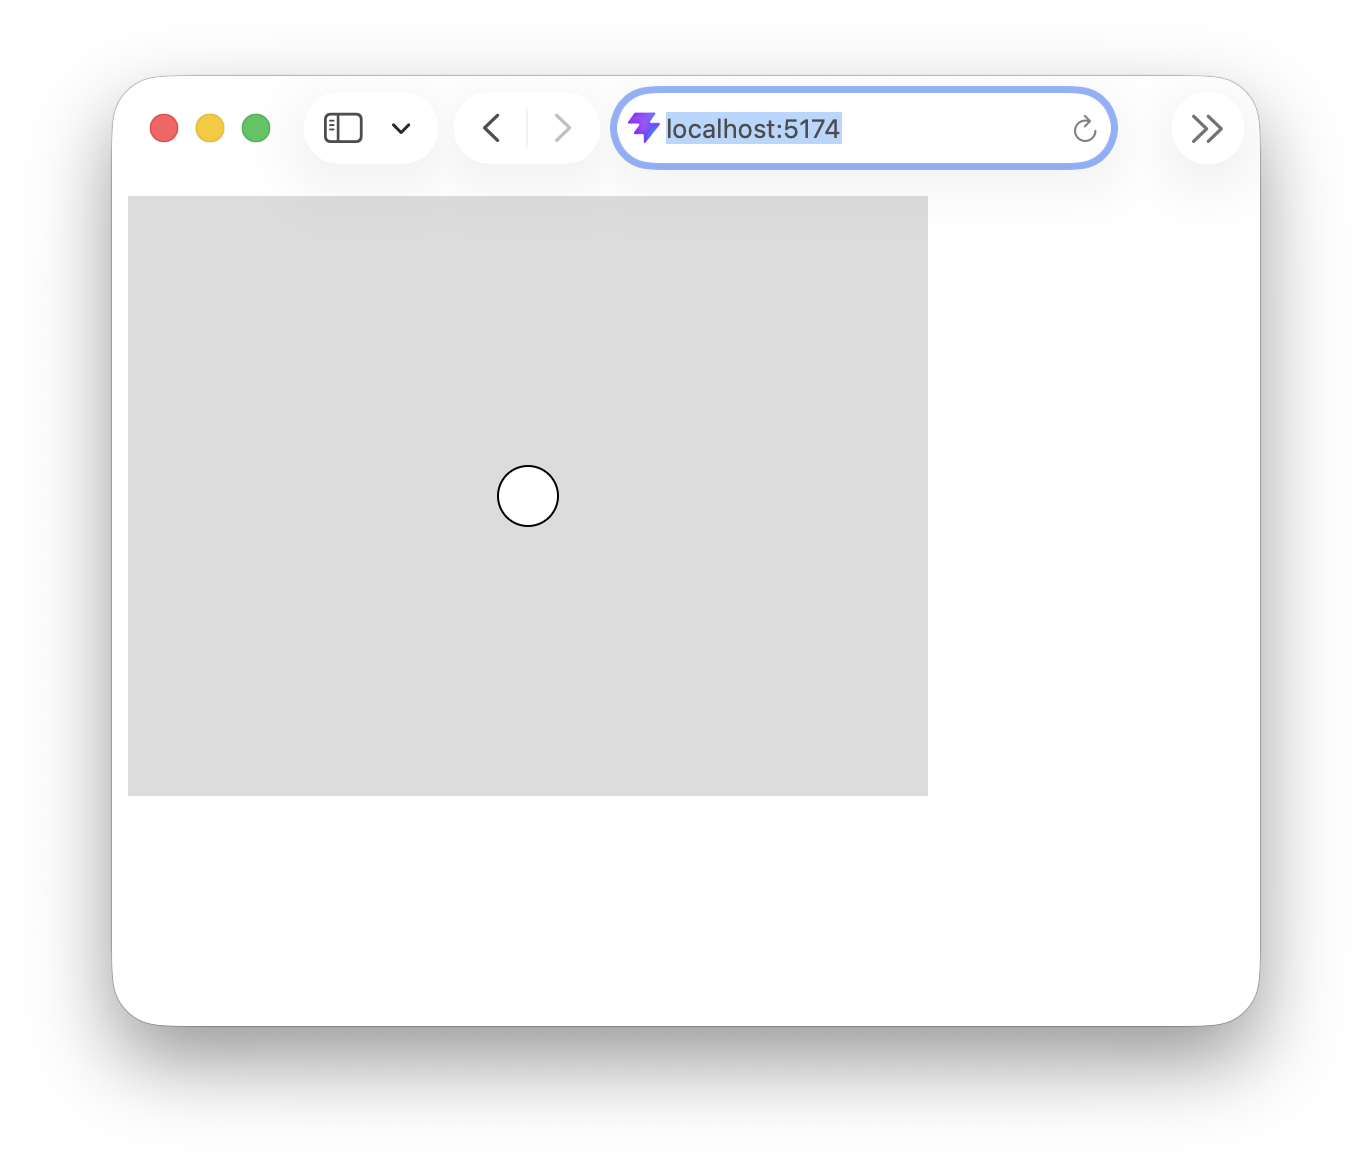
\includegraphics[width=0.5\textwidth]{figures/chapter01/browser-first-sketch.png}
    \caption{最初のスケッチの表示例}
    \label{fig:chapter01-first-sketch}
\end{figure}

5行目の\texttt{sketch}関数の引数名は、必ずしも\texttt{p}である必要はありません。
7行目や11行目で使っている\texttt{p.setup}や\texttt{p.draw}の\texttt{p}も、引数名を変えた場合は同じ名前にそろえます。
たとえば、引数名を\texttt{myP5}にした場合は、\texttt{myP5.createCanvas(...)}や\texttt{myP5.circle(...)}のように書きます（Listing~\ref{lst:chapter01-first-sketch-myP5}）。
慣習的に\texttt{p}という名前を使うのが慣習のようですので、この資料では\texttt{p}を使うことにします。

\begin{listing}[htbp]
\inputminted{ts}{listings/chapter01/first-sketch-myP5.ts}
\caption{最初のp5.jsスケッチの\texttt{p}を\texttt{myP5}に変更した例}
\label{lst:chapter01-first-sketch-myP5}
\end{listing}

\section{プログラムを書き換えてみよう}

プログラムが動いたら、少しだけ書き換えてみます。最初は、円の大きさ、円の位置、背景の色を変えるだけで十分です。この教材プロジェクトで最初に編集するファイルは、\texttt{typescript-p5/src/main.ts}です。
VS Codeのエクスプローラーで\texttt{typescript-p5}、\texttt{src}の順に開き、\texttt{main.ts}を選びます。そこで少しだけ数値を変えてみましょう。

たとえば、\texttt{p.circle(200, 150, 80)}の最後の数値を\texttt{120}に変えると、円が大きくなります。また、\texttt{p.background(240)}の数値を変えると、背景の明るさが変わります。

\begin{listing}[htbp]
\begin{minted}{ts}
p.background(220);
p.circle(200, 150, 120);
\end{minted}
\caption{背景と円の大きさを変更する例}
\label{lst:chapter01-edit-circle}
\end{listing}

別の章のサンプルを試すときは、VS Codeのエクスプローラーで\texttt{listings/}にある対象ファイルを開きます。開いた内容をすべて選んでコピーし、\texttt{typescript-p5/src/main.ts}を開いて内容をすべて選んで貼り付け、保存します。これにより\texttt{src/main.ts}の内容は上書きされます。

PowerShellを使う場合は、\texttt{typescript-p5/}を開いているターミナルで次のコマンドを実行します。

\begin{listing}[htbp]
\begin{minted}{powershell}
Copy-Item ..\listings\chapter02\points-and-lines.ts .\src\main.ts
\end{minted}
\caption{第2章のサンプルで\texttt{main.ts}を上書きするコマンド}
\label{lst:chapter01-copy-sample}
\end{listing}

\texttt{listings/}にあるファイルそのものは実行されません。コピーした\texttt{src/main.ts}が実行されます。保存またはコピーの後は、通常はViteを再起動しなくてもブラウザの表示が更新されます。画像、JSON、音を使うサンプルでは、それぞれの章で説明する素材ファイルも必要です。

書き換えたあとに期待どおりに動かないときは、まずVS Codeの赤い波線を確認します。次にターミナルの表示を確認し、最後にブラウザの表示を確認します。

\section{Gitで保存してみよう}

Gitでは、ファイルの変更を記録として保存できます。この記録をコミットと呼びます。コミットを作っておくと、あとで「どの時点で何を変更したか」を確認できます。この節では、開発サーバ用とは別にターミナルを開き、教材リポジトリのルートフォルダでGitコマンドを実行します。

まず、現在の変更状態を確認します。

\begin{listing}[htbp]
\begin{minted}{powershell}
git status
\end{minted}
\caption{Gitで変更状態を確認するコマンド}
\label{lst:chapter01-git-status}
\end{listing}

変更したファイルが表示されたら、次のように保存対象へ追加します。

\begin{listing}[htbp]
\begin{minted}{powershell}
git add typescript-p5/src/main.ts
\end{minted}
\caption{変更したファイルを保存対象へ追加するコマンド}
\label{lst:chapter01-git-add}
\end{listing}

この節ではGitコマンドを教材リポジトリのルートフォルダで実行します。一方、\texttt{npm}のコマンドは\texttt{typescript-p5/}で実行します。コマンドごとに実行する場所を確認しましょう。

最後に、変更内容を説明する短いメッセージを付けてコミットします。

\begin{listing}[htbp]
\begin{minted}{powershell}
git commit -m "最初のスケッチを変更"
\end{minted}
\caption{Gitで変更を保存するコマンド}
\label{lst:chapter01-git-commit}
\end{listing}

\begin{notebox}{コミットメッセージ}
コミットメッセージは、あとで見返したときに変更内容が分かるように書きます。最初は短い日本語で構いません。
\end{notebox}

\section{よくある間違い}

環境構築では、プログラムの文法とは別のところでつまずくことがあります。エラーが出たときは、あわてずに表示されたメッセージと作業しているフォルダを確認しましょう。

\begin{mistakebox}{コマンドを実行する場所が違う}
\texttt{npm install}や\texttt{npm run dev}は、教材プロジェクトのフォルダで実行します。\texttt{package.json}があるフォルダをVS Codeで開いているか確認してください。
\end{mistakebox}

\begin{mistakebox}{開発サーバを止めてしまう}
\texttt{npm run dev}を実行しているターミナルを閉じると、開発サーバも止まります。
作業中はそのターミナルを開いたままにしておきます。
止めたいときは、ターミナルで\texttt{Ctrl + C}を押します。
\end{mistakebox}

\begin{mistakebox}{Gitの保存とファイル保存を混同する}
VS Codeでファイルを保存することと、Gitでコミットすることは別の操作です。ファイル保存は現在の内容をディスクに書き込む操作で、コミットは変更の記録を作る操作です。
\end{mistakebox}

\section{まとめ}

この章では、Windows環境でTypeScript + p5.jsの教材を動かす準備をしました。VS Code、Git、Node.jsをインストールし、GitHubから教材を取得し、\texttt{npm install}と\texttt{npm run dev}でプログラムを実行しました。

また、最初のスケッチを少し書き換え、Gitで変更を保存する流れも確認しました。次章からは、p5.jsを使って図形を描く方法を少しずつ学んでいきます。

\section{演習問題}

この章の演習では、環境構築と最初の実行を確認します。すべてを暗記する必要はありません。コマンドを見ながら、同じ操作を自分のPCで再現できることを目指しましょう。

\begin{enumerate}
    \item VS Codeを起動し、教材フォルダを開いてください。
    \item VS Codeで新しいターミナルを開き、現在のフォルダが教材フォルダであることを確認してください。
    \item \texttt{node -v}と\texttt{npm -v}を実行し、バージョン番号が表示されることを確認してください。
    \item \texttt{npm install}を実行し、必要なライブラリをインストールしてください。
    \item \texttt{npm run dev}を実行し、ブラウザで教材ページを開いてください。
    \item 最初のスケッチで、円の大きさを変更してください。
    \item 最初のスケッチで、背景の明るさを変更してください。
    \item \texttt{git status}を実行し、変更されたファイルを確認してください。
    \item 変更したファイルを\texttt{git add}で追加し、\texttt{git commit}で保存してください。
    \item 挑戦問題として、円の位置、大きさ、背景色をすべて変更し、自分なりの最初の画面を作ってください。
\end{enumerate}

\chapter{図形を描く}
\label{chap:drawing-shapes}

この章では、p5.jsを使って点、線、円、長方形、三角形、四角形を描く方法を学びます。座標を使って図形の位置を決め、命令を並べる順番によって重なり方を考えながら、TypeScript + p5.js instance modeで図形を描いていきます。

\section{この章の概要}

コンピュータで絵を描くときには、「どこに」「どのような大きさで」描くかを数値で指定します。最初は数値が多く見えるかもしれませんが、どの数値が位置を表し、どの数値が大きさを表すのかを分けて考えると読みやすくなります。

この章で扱う主な内容は次の通りです。

\begin{itemize}
    \item サンプルを読むためのJavaScriptの短い復習
    \item キャンバスと座標の考え方
    \item 点と線の描き方
    \item 円、楕円、長方形の描き方
    \item 三角形と四角形の描き方
    \item 描く順番による見え方の違い
    \item 複数の図形を組み合わせる考え方
\end{itemize}

\section{JavaScriptの書き方を復習する}

第1章で動かしたスケッチには、JavaScriptやTypeScriptの記号がいくつか使われていました。以前にJavaScriptを学んだことがあっても、記号の意味をすぐに思い出せないことがあります。この節では、これからサンプルを読むために必要な部分だけを短く復習します。すべてを暗記する必要はなく、分からなくなったときにここへ戻って確認できれば十分です。

まず、サンプルでよく使う記号とインデントの読み方を確認します。

\begin{table}[H]
    \centering
    \caption{サンプルを読むために使う記号}
    \label{tab:chapter02-javascript-symbols}
    \begin{tabular}{p{0.13\linewidth}p{0.31\linewidth}p{0.46\linewidth}}
        \toprule
        記号 & 呼び方・使う場所 & 読み方 \\
        \midrule
        \texttt{\{ \}}
            & 波括弧
            & 関数などに含まれる処理の始まりと終わりを表します。対応する開き括弧と閉じ括弧を探します。 \\
        \texttt{( )}
            & 丸括弧
            & 関数を定義するときは受け取る値の名前を、呼び出すときは渡す値を書きます。\texttt{()}は、それらがないことを表します。 \\
        \texttt{;}
            & セミコロン
            & 1つの文の終わりを表します。本書のサンプルでは、文の最後に付けます。 \\
        インデント
            & 行の先頭の空白
            & どの処理が\texttt{\{ \}}の内側にあるかを見やすくします。同じ深さの行は、先頭をそろえます。 \\
        \bottomrule
    \end{tabular}
\end{table}

\texttt{p.circle(200, 150, 80);}のように、関数の名前の後ろへ丸括弧を書いたものは、\textbf{関数呼び出し}です。丸括弧の中に書く\texttt{200}、\texttt{150}、\texttt{80}のような値を\textbf{引数}と呼びます。この例では、\texttt{p.circle}関数へ、円の中心のx座標、中心のy座標、直径を順番に渡しています。

引数はコンマで区切り、関数ごとに個数と順番が決まっています。たとえば、\texttt{p.createCanvas(400, 300)}では、最初の引数がキャンバスの幅、次の引数が高さです。引数の詳しい考え方は、第8章「関数で整理する」で扱います。

値に名前を付けるときには、\texttt{const}または\texttt{let}を使います。途中で値を変えない場合は\texttt{const}、あとで値を変える場合は\texttt{let}を使います。

\begin{center}
\begin{tabular}{lll}
    \toprule
    書き方 & 意味 & 例 \\
    \midrule
    \texttt{const} & あとから別の値を代入しない & \texttt{const diameter: number = 80;} \\
    \texttt{let} & あとから値を変えることができる & \texttt{let circleX: number = 100;} \\
    \bottomrule
\end{tabular}
\end{center}

ここでは、サンプルの中で\texttt{const}と\texttt{let}を見分けられれば十分です。変数、型注釈、\texttt{const}と\texttt{let}の使い分けは、第4章「変数と型注釈」で詳しく説明します。

JavaScriptとTypeScriptでは、\texttt{=}と\texttt{===}の意味が異なります。

\begin{center}
\begin{tabular}{lll}
    \toprule
    記号 & 意味 & 例 \\
    \midrule
    \texttt{=} & 右側の値や処理を左側へ代入する & \texttt{circleX = 200;} \\
    \texttt{===} & 左右の値が等しいか比較する & \texttt{circleX === 200} \\
    \bottomrule
\end{tabular}
\end{center}

\texttt{circleX = 200;}は、\texttt{circleX}へ\texttt{200}を代入する文です。一方、\texttt{circleX === 200}は、値が等しければ\texttt{true}、等しくなければ\texttt{false}になる比較です。比較は、第6章「条件分岐とインタラクション」で詳しく扱います。

\texttt{//}から行の終わりまでは\textbf{コメント}です。コメントはプログラムの説明として人が読むためのもので、処理としては実行されません。本書では、変数が何を表すか、なぜその処理が必要かを示すためにコメントを使います。

プログラムに間違いがあると、VS Codeに赤い波線が表示されたり、ターミナルやブラウザにエラーメッセージが表示されたりします。最初から英語のメッセージをすべて理解する必要はありません。まず、ファイル名と行番号を探し、その行の括弧、セミコロン、関数名、引数の個数を確認しましょう。VS Codeの赤い波線へマウスポインタを重ねると、間違いの手掛かりが表示されます。

\begin{pointbox}{エラーは修正場所を探す手掛かり}
エラーメッセージは、失敗を知らせるだけのものではなく、どこを確認すればよいかを示す手掛かりです。最初に表示されたエラーのファイル名と行番号から確認し、修正したらもう一度保存して動作を確かめましょう。
\end{pointbox}

\section{キャンバスと座標}

p5.jsでは、図形を描くための領域をキャンバス\footnote{英語では、canvasと書きます。}と呼びます。
instance modeでは、スケッチを表す\texttt{p}を通して\texttt{p.createCanvas}を呼び出し、キャンバスを作ります。
\texttt{p.createCanvas(400, 300)}は、幅400、高さ300のキャンバスを作る命令です。

\begin{listing}[htbp]
\begin{minted}{ts}
p.createCanvas(400, 300);
\end{minted}
\caption{幅400、高さ300のキャンバスを作る}
\label{lst:chapter02-create-canvas}
\end{listing}

この例では、横400ピクセル、縦300ピクセルのキャンバスを作っています。ピクセル\footnote{英語では、pixelと書きます。日本語では画素と呼ぶこともあります。}とは、画面上の小さな点のことです。デジタル画像は、このピクセルの集まりとして表示されます。

\begin{figure}[htbp]
    \centering
    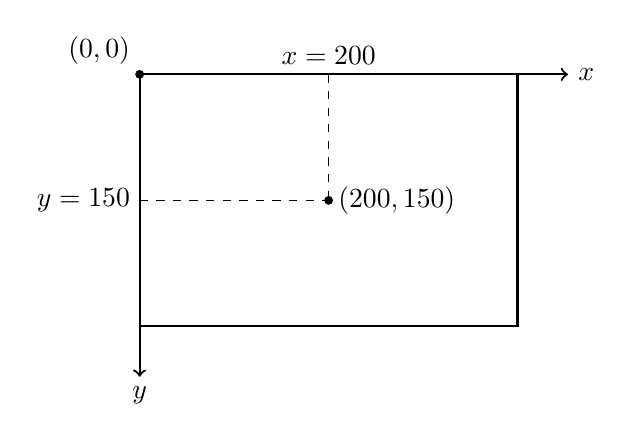
\begin{tikzpicture}[scale=0.8]
        \draw[thick] (0,0) rectangle (6,-4);    %%% ここを修正
        \draw[->,thick] (0,0) -- (6.8,0) node[right] {$x$};
        \draw[->,thick] (0,0) -- (0,-4.8) node[below] {$y$};
        \fill (0,0) circle (2pt);
        \node[above left] at (0,0) {$(0, 0)$};
        \fill (3,-2) circle (2pt);
        \node[right] at (3,-2) {$(200, 150)$};
        \draw[dashed] (3,0) -- (3,-2);
        \draw[dashed] (0,-2) -- (3,-2);
        \node[above] at (3,0) {$x=200$};
        \node[left] at (0,-2) {$y=150$};
    \end{tikzpicture}
    \caption{p5.jsの座標の考え方}
    \label{fig:chapter02-coordinate-system}
\end{figure}

画面上のピクセルの位置を表すために、高校まで数学で学んだグラフのように、水平方向に$X$軸、垂直方向に$Y$軸を考えます。
数学のグラフでは、右に進むほど $X$座標の値が大きくなり、上に進むほど $Y$座標の値が大きくなります。
一方、p5.jsなどのコンピュータの世界では、左上が原点で、下に進むほど $Y$座標の値が大きくなりますことが多いです（図\ref{fig:chapter02-coordinate-system}）。
この違いはとても重要です。

\section{点と線を描く}
\label{sec:points-and-lines}

点を描くには、その点の $X$ 座標と $Y$ 座標を指定します。
線を描くには、線分の始点と終点の $X$ 座標と $Y$ 座標を指定します。

\begin{listing}[htbp]
\inputminted{ts}{listings/chapter02/points-and-lines.ts}
\caption{点と線を描く}
\label{lst:chapter02-points-and-lines}
\end{listing}

9行目の\texttt{p.background(250)}は、キャンバスの背景を白に近い灰色で塗りつぶす命令です。
引数の数値は、0から255までの範囲で、0が黒、255が白のように明るさが変化します。
\texttt{p.point(80, 80)}は、$X$ 座標が80、$Y$ 座標が80の位置に点を描きます。\texttt{p.line(80, 80, 320, 220)}は、$(80, 80)$から$(320, 220)$までの線分を描きます。
また、点や線の太さを変えるには、\texttt{strokeWeight}関数を使います。
引数に指定した数値が大きいほど、点や線は太くなります。
例えば、11行目の\texttt{p.strokeWeight(8)}により点を見やすくし、その後、16行目の\texttt{p.strokeWeight(2)}で線を少し細くしてから線分を描いています。

8行目から17行目で指定された命令は、上から順に実行されます。
7行目から18行目では、最初に1回だけ実行される\texttt{setup}関数を定義していることになっています。

Javascriptの事をよく知っている人には、このサンプルの7行目から18行目は、JavaScriptのアロー関数を使った書き方で、
関数\texttt{setup}の定義を行っていると言った方が簡単に理解できるかもしれません。
同じように、5行目から19行目では、\texttt{sketch}関数の定義を行っています。

この節で使われた関数をまとめると、次の表のようになります。

\begin{table}[htbp]
\centering
\begin{tabular}{ll}
\toprule
関数 & 説明 \\
\midrule
\texttt{setup()} & 1回だけ実行される初期化用の関数、動作はプログラムが決める \\
\texttt{createCanvas(w, h)} & 幅$w$、高さ$h$のキャンバスを作る \\
\texttt{background(gray)} & キャンバスを灰色の明るさ$gray$で塗りつぶす \\
\texttt{point(x, y)} & 座標$(x, y)$に点を描く \\
\texttt{line(x1, y1, x2, y2)} & 座標$(x1, y1)$から$(x2, y2)$までの線分を描く \\
\texttt{strokeWeight(w)} & 線の太さや点の大きさを$w$にする \\
\bottomrule
\end{tabular}
\caption{節\ref{sec:points-and-lines}で使った関数}
\label{tab:chapter02-points-and-lines}
\end{table}

表\ref{tab:chapter02-points-and-lines}で紹介した\texttt{point}、\texttt{line}、\texttt{strokeWeight}は、図\ref{fig:chapter02-point-line-strokeweight}のような関係にあります。
\texttt{point}は1つの座標に点を置き、\texttt{line}は2つの座標を結びます。
\texttt{strokeWeight}は、その後に描く点や線の太さを変える命令です。

\begin{figure}[htbp]
    \centering
    \begin{tikzpicture}[x=1cm, y=1cm, font=\small]
        \tikzset{
            canvas/.style={draw=black!70, fill=gray!5, line width=0.6pt},
            guide/.style={draw=gray!35, dashed, line width=0.4pt},
            markpoint/.style={fill=black},
            labeltext/.style={font=\small\ttfamily}
        }

        \begin{scope}[shift={(0,0)}]
            \draw[canvas] (0,0) rectangle (3.5,-2.4);
            \draw[guide] (1.75,0) -- (1.75,-1.2);
            \draw[guide] (0,-1.2) -- (1.75,-1.2);
            \fill[markpoint] (1.75,-1.2) circle (2.2pt);
            \node[labeltext] at (1.75,-2.85) {point(x, y)};
            \node[align=center] at (1.75,-3.35) {指定した座標に\\点を描く};
        \end{scope}

        \begin{scope}[shift={(4.4,0)}]
            \draw[canvas] (0,0) rectangle (3.5,-2.4);
            \fill[markpoint] (0.7,-0.6) circle (1.8pt);
            \fill[markpoint] (2.8,-1.8) circle (1.8pt);
            \draw[line width=1.1pt] (0.7,-0.6) -- (2.8,-1.8);
            \node[above right, font=\scriptsize] at (0.7,-0.6) {$(x_1,y_1)$};
            \node[below left, font=\scriptsize] at (2.8,-1.8) {$(x_2,y_2)$};
            \node[labeltext] at (1.75,-2.85) {line(x1, y1, x2, y2)};
            \node[align=center] at (1.75,-3.35) {始点と終点を\\線で結ぶ};
        \end{scope}

        \begin{scope}[shift={(8.8,0)}]
            \draw[canvas] (0,0) rectangle (3.5,-2.4);
            \draw[line width=0.5pt] (0.45,-0.55) -- (1.45,-0.55);
            \draw[line width=2.6pt] (2.05,-0.55) -- (3.05,-0.55);
            \fill[markpoint] (0.95,-1.55) circle (1.2pt);
            \fill[markpoint] (2.55,-1.55) circle (4.5pt);
            \node[font=\scriptsize] at (0.95,-0.95) {$w=1$};
            \node[font=\scriptsize] at (2.55,-0.95) {$w=8$};
            \node[labeltext] at (1.75,-2.85) {strokeWeight(w)};
            \node[align=center] at (1.75,-3.35) {点や線の\\太さを変える};
        \end{scope}
    \end{tikzpicture}
    \caption{\texttt{point}、\texttt{line}、\texttt{strokeWeight}の働き}
    \label{fig:chapter02-point-line-strokeweight}
\end{figure}

\begin{notebox}{点が小さく見えるとき}
点はそのままだと小さく見えます。このサンプルでは、見やすくするために\texttt{p.strokeWeight(8)}で点や線の太さを変えています。線の太さや色の詳しい指定は、次の章で扱います。
\end{notebox}

\section{円、楕円、長方形を描く}

円や長方形も、位置と大きさを数値で指定して描きます。最初は、中心を指定する図形と、左上の位置を指定する図形の違いに注意しましょう。

\begin{listing}[htbp]
\inputminted{ts}{listings/chapter02/ellipses-and-rectangles.ts}
\caption{円、楕円、長方形を描く}
\label{lst:chapter02-ellipses-and-rectangles}
\end{listing}

\texttt{p.ellipse(120, 120, 160, 120)}は、中心が$(120, 120)$、幅が160、高さが120の楕円を描きます。\texttt{p.circle(300, 120, 100)}は、中心が$(300, 120)$、直径が100の円を描きます。

\texttt{p.rect(360, 70, 80, 100)}は、左上の位置が$(360, 70)$、幅が80、高さが100の長方形を描きます。円や楕円と長方形では、最初の2つの数値の意味が少し違います。

この節で使われた関数をまとめると、次の表のようになります。

\begin{table}[htbp]
\centering
\begin{tabular}{ll}
\toprule
関数 & 説明 \\
\midrule
\texttt{ellipse(x, y, w, h)} & 中心$(x, y)$、幅$w$、高さ$h$の楕円を描く \\
\texttt{circle(x, y, d)} & 中心$(x, y)$、直径$d$の円を描く \\
\texttt{rect(x, y, w, h)} & 左上の位置$(x, y)$、幅$w$、高さ$h$の長方形を描く \\
\bottomrule
\end{tabular}
\caption{円、楕円、長方形を描く関数}
\label{tab:chapter02-ellipses-and-rectangles}
\end{table}

表\ref{tab:chapter02-ellipses-and-rectangles}で紹介した3つの関数は、図\ref{fig:chapter02-ellipse-circle-rect}のような図形を描きます。
\texttt{ellipse}と\texttt{circle}は中心の位置を決めてから図形の大きさを指定します。
一方、\texttt{rect}は左上の位置を決めてから、右方向の幅と下方向の高さを指定します。

\begin{figure}[htbp]
    \centering
    \begin{tikzpicture}[x=0.95cm, y=0.95cm, font=\small]
        \tikzset{
            canvas/.style={draw=black!70, fill=gray!5, line width=0.6pt},
            guide/.style={draw=gray!40, dashed, line width=0.4pt},
            drawnshape/.style={draw=black, fill=gray!18, line width=1pt},
            basepoint/.style={fill=black},
            labeltext/.style={font=\small\ttfamily}
        }

        \begin{scope}[shift={(0,0)}]
            \draw[canvas] (0,0) rectangle (3.5,-2.6);
            \draw[drawnshape] (1.75,-1.25) ellipse (1.15 and 0.65);
            \draw[guide] (0.6,-1.25) -- (2.9,-1.25);
            \draw[guide] (1.75,-0.6) -- (1.75,-1.9);
            \fill[basepoint] (1.75,-1.25) circle (2pt);
            \node[above, font=\scriptsize] at (1.75,-1.25) {中心};
            \draw[<->, font=\scriptsize] (0.6,-2.15) -- node[below] {$w$} (2.9,-2.15);
            \draw[<->, font=\scriptsize] (3.1,-0.6) -- node[right] {$h$} (3.1,-1.9);
            \node[labeltext] at (1.75,-3.05) {ellipse(x, y, w, h)};
            \node[align=center] at (1.75,-3.55) {中心と幅・高さで\\楕円を描く};
        \end{scope}

        \begin{scope}[shift={(4.4,0)}]
            \draw[canvas] (0,0) rectangle (3.5,-2.6);
            \draw[drawnshape] (1.75,-1.25) circle (0.75);
            \draw[guide] (1.0,-1.25) -- (2.5,-1.25);
            \fill[basepoint] (1.75,-1.25) circle (2pt);
            \node[above, font=\scriptsize] at (1.75,-1.25) {中心};
            \draw[<->, font=\scriptsize] (1.0,-2.15) -- node[below] {$d$} (2.5,-2.15);
            \node[labeltext] at (1.75,-3.05) {circle(x, y, d)};
            \node[align=center] at (1.75,-3.55) {中心と直径で\\円を描く};
        \end{scope}

        \begin{scope}[shift={(8.8,0)}]
            \draw[canvas] (0,0) rectangle (3.5,-2.6);
            \draw[drawnshape] (0.85,-0.65) rectangle (2.75,-1.9);
            \fill[basepoint] (0.85,-0.65) circle (2pt);
            \node[above right, font=\scriptsize] at (0.85,-0.65) {左上};
            \draw[<->, font=\scriptsize] (0.85,-2.15) -- node[below] {$w$} (2.75,-2.15);
            \draw[<->, font=\scriptsize] (3.0,-0.65) -- node[right] {$h$} (3.0,-1.9);
            \node[labeltext] at (1.75,-3.05) {rect(x, y, w, h)};
            \node[align=center] at (1.75,-3.55) {左上と幅・高さで\\長方形を描く};
        \end{scope}
    \end{tikzpicture}
    \caption{\texttt{ellipse}、\texttt{circle}、\texttt{rect}で描かれる図形}
    \label{fig:chapter02-ellipse-circle-rect}
\end{figure}

\begin{pointbox}{中心で指定する図形と左上で指定する図形}
\texttt{ellipse}や\texttt{circle}は中心の座標を指定します。\texttt{rect}は基本的に左上の座標を指定します。どの点を基準にしているかを意識すると、図形を配置しやすくなります。
\end{pointbox}

\section{三角形と四角形を描く}

三角形や四角形は、頂点の座標を順番に指定して描きます。少し数値が多くなりますが、「1つの頂点に$x$と$y$の2つの数値が必要」と考えると整理しやすくなります。

\begin{listing}[htbp]
\inputminted{ts}{listings/chapter02/triangles-and-quads.ts}
\caption{三角形と四角形を描く}
\label{lst:chapter02-triangles-and-quads}
\end{listing}

\begin{figure}[http]
    \centering
    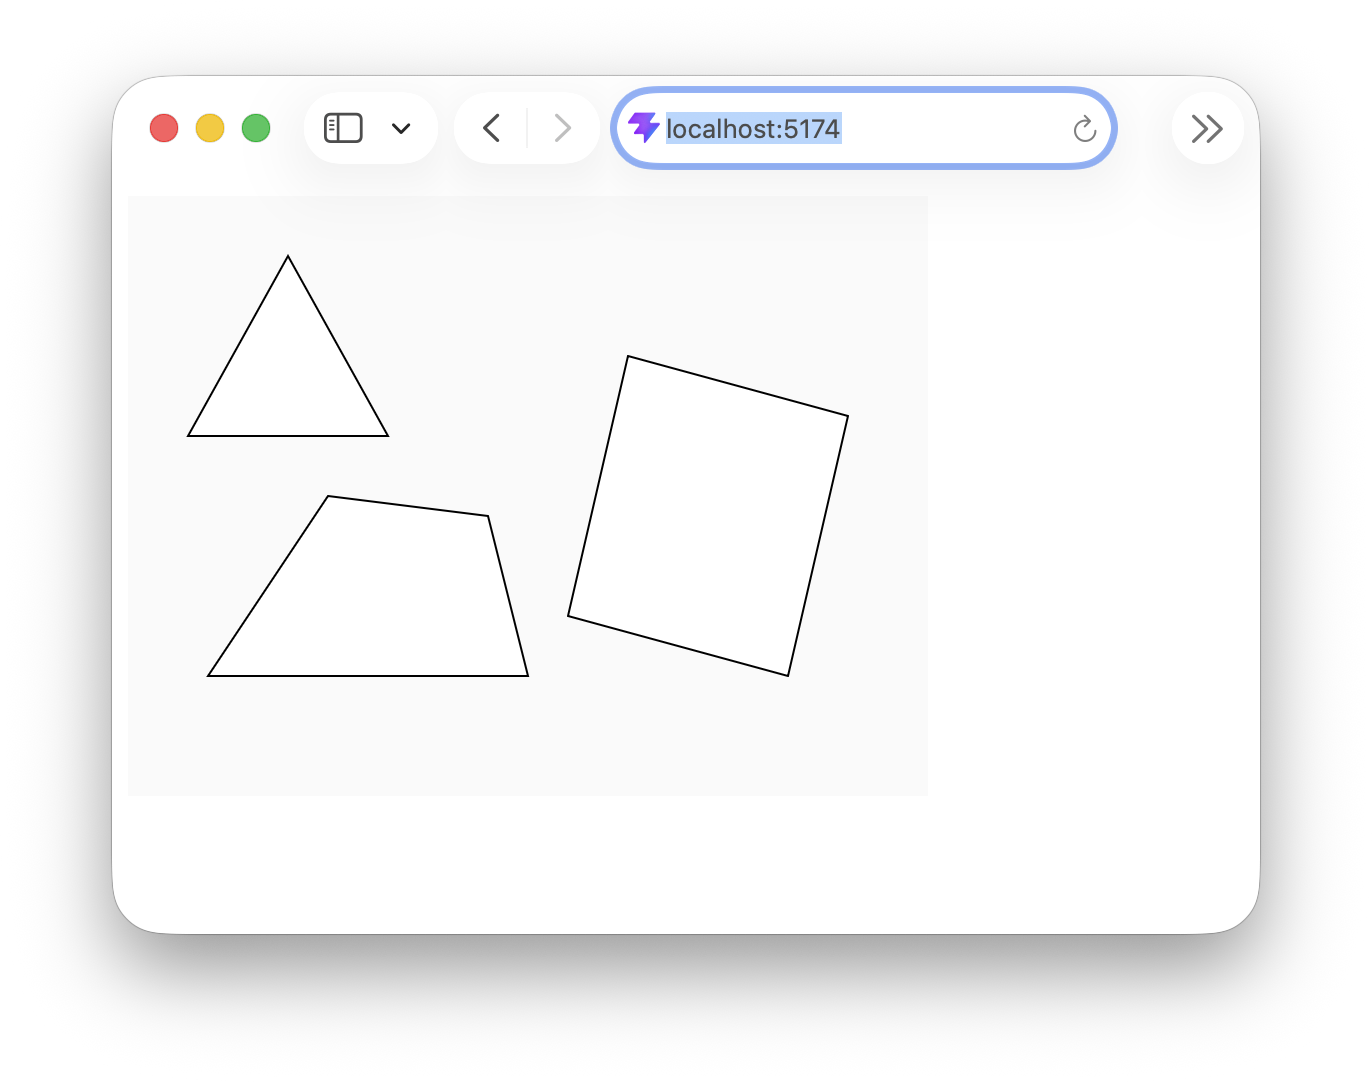
\includegraphics[width=0.6\linewidth]{figures/chapter02/triangle-quad.png}
    \caption{三角形と四角形の描画例}
    \label{fig:chapter02-triangle-quad}
\end{figure}

\texttt{triangle}関数では3つの頂点を指定します。つまり、合計で6つの数値を使います。
\texttt{quad}関数では4つの頂点を指定するため、合計で8つの数値を使います。
\texttt{rect}関数は、長方形（矩形）を描くための関数ですが、\texttt{quad}関数では、台形のような形も描くことができます。

\begin{table}[htbp]
\centering
\begin{tabular}{lp{0.52\linewidth}}
\toprule
関数 & 説明 \\
\midrule
\texttt{triangle(x1, y1, x2, y2,x3, y3)} & 3つの頂点$(x1, y1)$、$(x2, y2)$、$(x3, y3)$を結んで三角形を描く \\
\shortstack[l]{\texttt{quad(x1, y1, x2, y2,x3, y3,}\\\texttt{ x4, y4)}} & 4つの頂点$(x1, y1)$、$\cdots$、$(x4, y4)$を結んで四角形を描く \\
\bottomrule
\end{tabular}
\caption{三角形と四角形を描く関数}
\label{tab:chapter02-triangles-and-quads}
\end{table}

\begin{notebox}{数値が増えたときの読み方}
\texttt{p.triangle(30, 120, 80, 30, 130, 120)}は、$(30, 120)$、$(80, 30)$、$(130, 120)$の3点をつないで三角形を描きます。2つずつ区切って読むのがコツです。
\end{notebox}

\section{描画順を考える}

p5.jsでは、命令は上から順に実行されます。後から描いた図形は、前に描いた図形の上に重なって表示されます。

\begin{listing}[htbp]
\inputminted{ts}{listings/chapter02/drawing-order.ts}
\caption{描く順番で見え方が変わる例}
\label{lst:chapter02-drawing-order}
\end{listing}

このサンプルでは、先に長方形を描き、その後に円を描いています。そのため、重なっている部分では円が上に見えます。もし命令の順番を入れ替えると、長方形が円の上に描かれます。

\section{図形を組み合わせる}

点、線、円、三角形を組み合わせると、簡単な絵を作ることができます。まだ色を詳しく扱っていないので、この章では形だけで顔のような絵を作ります。

\begin{listing}[htbp]
\inputminted{ts}{listings/chapter02/simple-face.ts}
\caption{複数の図形を組み合わせて顔を描く}
\label{lst:chapter02-simple-face}
\end{listing}

\begin{figure}[http]
    \centering
    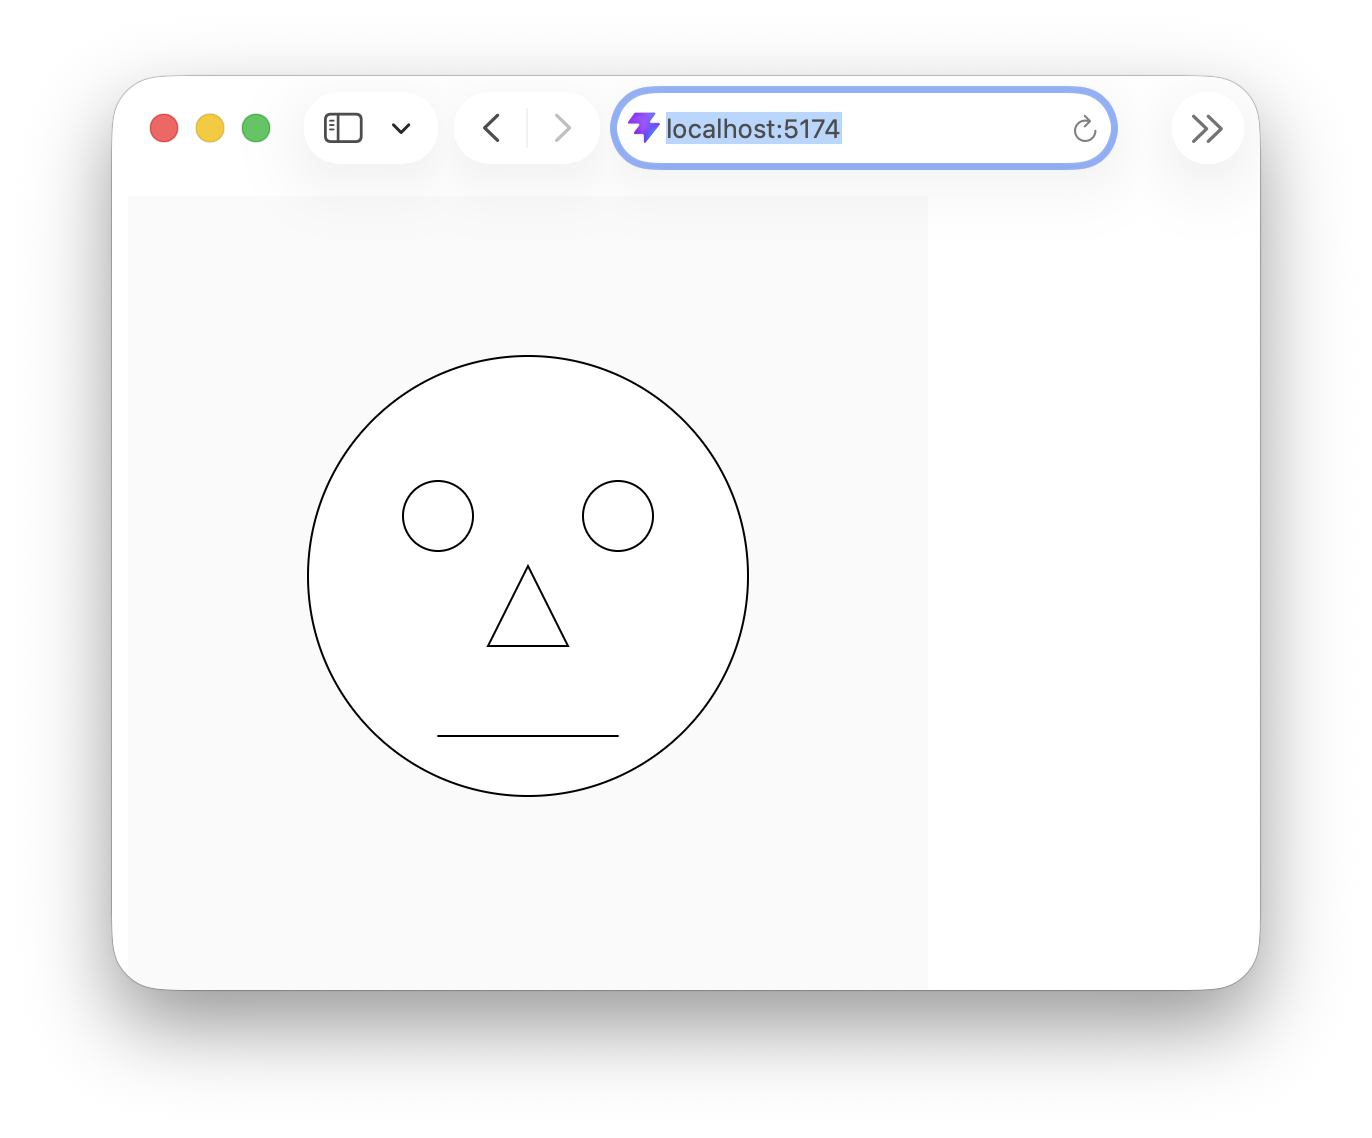
\includegraphics[width=0.6\linewidth]{figures/chapter02/simple-face.png}
    \caption{\ref{lst:chapter02-simple-face}の実行例}
    \label{fig:chapter02-simple-face}
\end{figure}

このサンプルでは、大きな円を顔、小さな円を目、三角形を鼻、線を口として使っています。図形を組み合わせるときには、まず大きな部品を描き、その後に細かい部品を重ねると考えやすくなります。

\begin{notebox}{circleについて}
\texttt{p.circle(x, y, d)}の3つ目の値は、半径ではなく直径です。たとえば、半径40の円を描きたいときは、3つ目に\texttt{80}を指定します。
\end{notebox}

\section{よくある間違い}

図形を描くプログラムでは、文法の間違いだけでなく、座標や数値の意味を取り違えることでも思った通りに表示されなくなります。

\begin{mistakebox}{y座標の向きを数学と同じだと思ってしまう}
p5.jsでは、下に進むほど$y$の値が大きくなります。上に動かしたいときは$y$を小さくし、下に動かしたいときは$y$を大きくします。
\end{mistakebox}

\begin{mistakebox}{rectの最初の2つの数値を中心だと思ってしまう}
\texttt{rect}の最初の2つの数値は、基本的に左上の座標です。\texttt{ellipse}や\texttt{circle}の中心座標とは意味が違います。
\end{mistakebox}

\begin{mistakebox}{p.を付け忘れる}
instance modeでは、\texttt{circle(...)}ではなく\texttt{p.circle(...)}のように書きます。p5.jsの命令を使うときは、前に\texttt{p.}を付けることを確認しましょう。
\end{mistakebox}

\begin{mistakebox}{描く順番を意識していない}
後から描いた図形は前に描いた図形の上に重なります。図形が隠れてしまったときは、命令の順番を見直しましょう。
\end{mistakebox}

\section{まとめ}

この章では、p5.jsで基本的な図形を描く方法を学びました。キャンバスは\texttt{p.createCanvas}で作り、点、線、円、楕円、長方形、三角形、四角形をそれぞれ専用の命令で描きます。

また、p5.jsの座標では左上が原点で、下に進むほど$y$の値が大きくなることを確認しました。さらに、図形は命令の順番通りに描かれ、後から描いた図形が手前に見えることも学びました。

\section{演習問題}

この章の演習では、座標と基本図形の描き方を確認します。最初はサンプルの数値を少し変えるところから始め、最後は複数の図形を組み合わせて自分の絵を作ってみましょう。

\begin{pointbox}{関数名と実際のコードの書き方}
本書では、関数の名前そのものを説明するときは、\texttt{point}関数や\texttt{line}関数のように書きます。
一方、TypeScript + p5.js instance modeのプログラムとして書くときは、\texttt{p.point(...)}や\texttt{p.line(...)}のように、前に\texttt{p.}を付けます。
演習で\texttt{point}関数と書かれている場合も、実際のコードでは\texttt{p.point(...)}の形で書いてください。
\end{pointbox}

\begin{enumerate}
    \item \texttt{p.createCanvas(400, 300)}の数値を変えて、横長のキャンバスと縦長のキャンバスを作ってください。
    \item \texttt{point}関数を3回以上使い、キャンバスの別々の場所に点を描いてください。
    \item \texttt{line}関数を使い、左上から右下へ向かう線と、左下から右上へ向かう線を描いてください。
    \item \texttt{circle}関数の直径を変えて、大きい円と小さい円を描いてください。
    \item \texttt{ellipse}関数を使い、横長の楕円と縦長の楕円を描いてください。
    \item \texttt{rect}関数を使い、同じ大きさの長方形を3つ、別々の位置に描いてください。
    \item \texttt{triangle}関数の頂点の数値を変えて、細長い三角形を作ってください。
    \item サンプルプログラム~\ref{lst:chapter02-drawing-order}で、描画順を入れ替えて、円が長方形の上に見える場合と、長方形が円の上に見える場合を比べてください。
    \item 円、三角形、線を組み合わせて、顔以外の簡単な絵を作ってください。
    \item 挑戦問題として、家、ロボット、乗り物など、複数の図形を組み合わせた作品を1つ作ってください。
\end{enumerate}

\chapter{色と見た目を変える}
\label{chap:color-and-style}

この章では、図形の色、枠線、塗りつぶし、線の太さを変える方法を学びます。第2章では図形の形と位置を中心に扱いました。ここでは、同じ図形でも色や線の指定によって印象が大きく変わることを確認します。

\section{この章の概要}

p5.jsでは、図形を描く前に色や線の設定を行います。設定した色や線の太さは、次に別の設定をするまで残ります。この「設定が残る」という考え方を理解すると、複数の図形を意図した見た目で描けるようになります。

この章で扱う主な内容は次の通りです。

\begin{itemize}
    \item RGBによる色の指定
    \item 灰色系の簡単な指定
    \item \texttt{fill}による塗りつぶし色の指定
    \item \texttt{stroke}と\texttt{strokeWeight}による枠線の指定
    \item \texttt{noFill}と\texttt{noStroke}の使い方
    \item 透明度を使った色の重なり
\end{itemize}

\section{RGBで色を指定する}

コンピュータの画面はピクセルで構成されていますが、
このピクセルの色は赤（Red）、緑（Green）、青（Blue）の光の強さとして表します\footnote{このように複数の色の組合せで色を表す方法を加法混色と呼びます。赤、緑、青の組合せで色を表す方法をRGB表色系と呼びます。}。
この3つを、英語の頭文字を取ってRGBと呼びます。

p5.jsでは、赤、緑、青の強さを0から255までの数値で指定します。
0はその色の成分がないことを表し、255はその色の成分の最も強い色であることを示しています。

\begin{listing}[htbp]
\inputminted{ts}{listings/chapter03/rgb-colors.ts}
\caption{RGBで赤、緑、青の円を描く}
\label{lst:chapter03-rgb-colors}
\end{listing}

\texttt{p.fill(255, 0, 0)}は、赤を強くし、緑と青を0にした色です。同じように、\texttt{p.fill(0, 180, 0)}は緑系の色、\texttt{p.fill(0, 80, 255)}は青系の色になります。

\begin{pointbox}{RGBの数値}
RGBの値は、基本的に\texttt{0}から\texttt{255}までの数値で指定します。赤、緑、青の3つの数値の組み合わせで、多くの色（$2^{24}$色）を表すことができます。
場合によっては、\texttt{0.0}から\texttt{1.0}までの小数で指定することもあります。
\end{pointbox}

\section{灰色を簡単に指定する}

白、黒、灰色のように色味のない色\footnote{このような色は無彩色と呼ばれます。}では、
赤、緑、青の値が同じになります。そのため、p5.jsでは同じ数値を3つ書く代わりに、1つの数値だけで灰色系の色を指定できます。

\begin{listing}[htbp]
\inputminted{ts}{listings/chapter03/grayscale-colors.ts}
\caption{1つの数値で灰色系の色を指定する}
\label{lst:chapter03-grayscale-colors}
\end{listing}

\texttt{p.fill(30,30,30)}の代わりに\texttt{p.fill(30)}と書くことができて、
\texttt{p.fill(30)}は黒に近い灰色、
\texttt{p.fill(130)}は中間の灰色、
\texttt{p.fill(220)}は白に近い灰色です。
\texttt{p.background(255,255,255)}の場合も、
代わりに\texttt{p.background(255)}と書くことが出来ます。
\texttt{p.fill(255)}と\texttt{p.fill(255, 255, 255)}は、どちらも白を表します。

\section{塗りつぶし色と枠線を指定する}

p5.jsの命令で描かれる円や長方形などの図形は、枠線とその内部の2つの部分に分かれています
（図\ref{fig:chapter03-fill-and-stroke-parts}参照）。
この2つの部分の色を別々に指定することができます。
内部の色は塗り潰し色と呼ばれ、\texttt{fill}関数で指定します。
枠線の色は\texttt{stroke}関数で指定し、枠線の太さは\texttt{strokeWeight}関数で指定します。

\begin{figure}[htbp]
    \centering
    \begin{tikzpicture}[x=1cm, y=1cm, font=\small]
        \tikzset{
            shapeFill/.style={fill=yellow!45},
            shapeStroke/.style={draw=blue!70!black, line width=5pt},
            guide/.style={draw=black!55, -stealth, line width=0.7pt},
            labelbox/.style={
                draw=black!45,
                fill=white,
                rounded corners=2pt,
                inner xsep=6pt,
                inner ysep=4pt,
                align=center
            }
        }

        \draw[shapeStroke, shapeFill] (0,0) rectangle (4,-2.4);

        \node[labelbox] (fillLabel) at (2,-3.35) {塗りつぶし\\\texttt{fill(...)}};
        \node[labelbox] (strokeLabel) at (5.65,-0.45) {枠線の色\\\texttt{stroke(...)}};
        \node[labelbox] (weightLabel) at (5.65,-1.75) {枠線の太さ\\\texttt{strokeWeight(...)}};

        \draw[guide] (fillLabel.north) -- (2,-1.2);
        \draw[guide] (strokeLabel.west) -- (4,-0.25);
        \draw[guide] (weightLabel.west) -- (4,-1.25);

        \node[align=center] at (2,0.65) {1つの図形は\\内側と外側に分けて考える};
    \end{tikzpicture}
    \caption{図形を構成する塗りつぶしと枠線}
    \label{fig:chapter03-fill-and-stroke-parts}
\end{figure}

\begin{listing}[htbp]
\inputminted{ts}{listings/chapter03/fill-and-stroke.ts}
\caption{塗りつぶし色、枠線の色、枠線の太さを変える}
\label{lst:chapter03-fill-and-stroke}
\end{listing}

このサンプルでは、円を描く前に青系の枠線、太さ6、黄色系の塗りつぶしを指定しています。その後、長方形を描く前に枠線と塗りつぶしを別の色に変更しています。

\begin{notebox}{設定は図形を描く前に書く}
\texttt{fill}関数や\texttt{stroke}関数は、すでに描いた図形の色を後から変える命令ではありません。これから描く図形に使う色を指定する命令です。
\end{notebox}

\section{塗りつぶしや枠線を消す}

図形によっては、塗りつぶしをなくして枠線だけにしたり、枠線をなくして塗りつぶしだけにしたりしたいことがあります。
そのようなときには、\texttt{noFill}関数と\texttt{noStroke}関数を使います。

\begin{listing}[htbp]
\inputminted{ts}{listings/chapter03/no-fill-and-no-stroke.ts}
\caption{塗りつぶしや枠線を消す}
\label{lst:chapter03-no-fill-and-no-stroke}
\end{listing}

左の円は\texttt{p.noFill()}によって塗りつぶしがなくなり、枠線だけで描かれます。右の円は\texttt{p.noStroke()}によって枠線がなくなり、塗りつぶしだけで描かれます。

\begin{mistakebox}{noFillとnoStrokeを同時に使う}
\texttt{p.noFill()}と\texttt{p.noStroke()}を両方指定すると、塗りつぶしも枠線もなくなります。その状態で図形を描いても、画面には何も見えません。
\end{mistakebox}

\section{色の設定は残る}

\texttt{fill}関数や\texttt{stroke}関数で指定した設定は、次に変更するまで残ります。
色鉛筆で絵を描く際に、一度ある色の鉛筆を使うと、次に別の色の鉛筆を使うまで同じ色で描き続けることと同じです。
これは便利ですが、どこで設定を変えたのかを見失うと、思っていない色で図形が描かれる原因にもなります。

\begin{listing}[htbp]
\inputminted{ts}{listings/chapter03/color-state.ts}
\caption{色の設定が次の図形にも使われる例}
\label{lst:chapter03-color-state}
\end{listing}

このサンプルでは、最初に\texttt{p.fill(255, 120, 80)}を指定しています。そのため、続けて描いた円と長方形は同じ色になります。その後で\texttt{p.fill(80, 150, 255)}を指定しているので、最後の円だけ別の色になります。

\begin{pointbox}{状態として残る設定}
\texttt{fill}、\texttt{stroke}、\texttt{strokeWeight}、\texttt{noFill}、\texttt{noStroke}の設定は、次の図形にも影響します。見た目がおかしいときは、図形の直前の設定を確認しましょう。
\end{pointbox}

\section{透明度を指定する}

図形の上に別な図形を描画すると、最初に描かれていた図形は完全に塗りつぶされてしまい、消えてしまいます。
このように、最初に描かれた図形を完全に消えてしまうことを防ぐために、不透明度付きの色を利用します。不透明度の値を小さくすると、その下に描かれている図形が透けて見えるようになります。
この不透明度のことをアルファ値と呼びます。

RGBの3つの数値に加えて、4つ目の数値を指定すると不透明度を指定できます。
アルファ値は、0に近いほど透明になり、255に近いほど不透明になります。

アルファ値を指定した場合の色の描画色は、次の式で計算されます\footnote{この式はRGBの各成分に対して適用されます。この式は、色の成分の値が0〜255の場合となります。}。
\[
\text{描画色} = \frac{\text{アルファ値}}{255} \times \text{指定した色} + \left(1 - \frac{\text{アルファ値}}{255}\right) \times \text{下の色}
\]

\begin{listing}[htbp]
\inputminted{ts}{listings/chapter03/transparent-colors.ts}
\caption{透明度を指定して色を重ねる}
\label{lst:chapter03-transparent-colors}
\end{listing}

\texttt{p.fill(255, 0, 0, 150)}は、赤に透明度を加えた指定です。円が重なっている部分では、後から描いた青い円だけでなく、下にある赤い円の色も見えます。

別なサンプルプログラムを紹介します。

\begin{listing}[htbp]
\inputminted{ts}{listings/chapter03/transparent-color-wrapped.ts}
\caption{透明度を指定して色を重ねる（別の例）}
\label{lst:chapter03-transparent-color-wrapped}
\end{listing}

\begin{figure}[htbp]
    \centering
    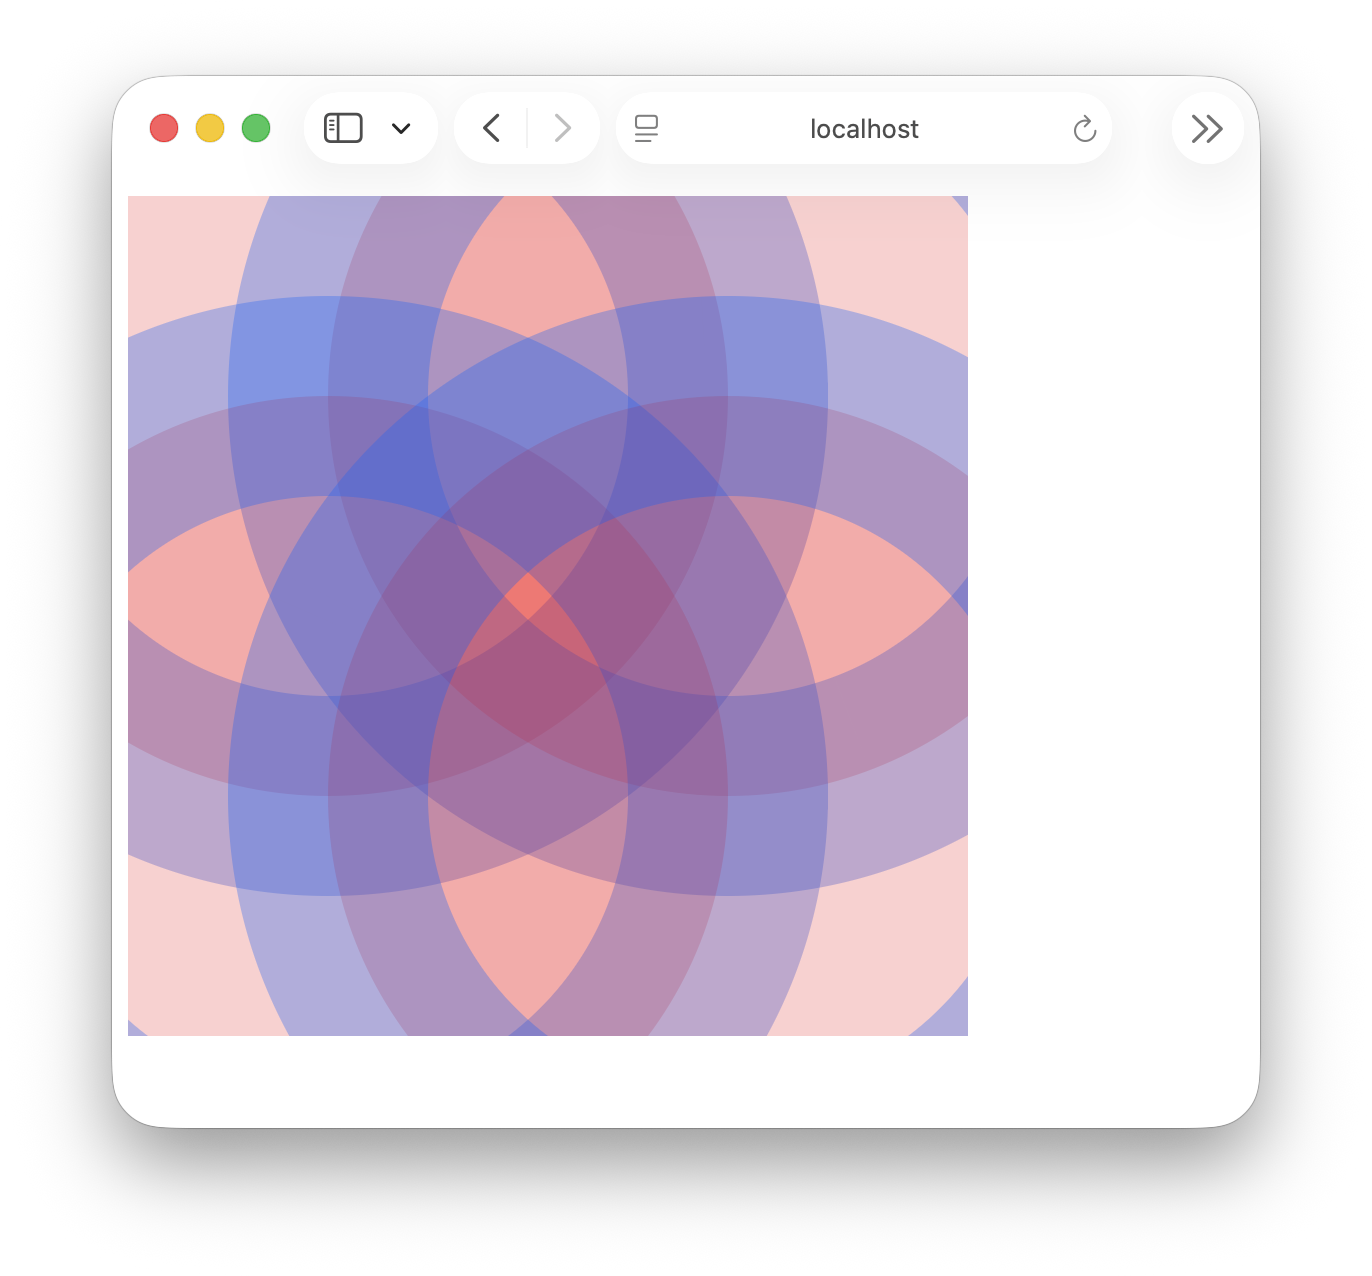
\includegraphics[width=0.5\linewidth]{figures/chapter03/transparent-color-wrapped.png}
    \caption{透明度を指定して色を重ねる（別の例）}
    \label{fig:chapter03-transparent-color-wrapped}
\end{figure}

\begin{notebox}{透明度は少しずつ試す}
透明度の値は、最初は\texttt{80}、\texttt{150}、\texttt{220}のように大きく変えて試すと違いが分かりやすくなります。
\end{notebox}

\section{色を使って顔を描く}

第2章では、円、三角形、線を組み合わせて顔のような絵を描きました。
ここでは、その絵に色と線の太さを加えて、より見た目を分かりやすくします。

\begin{listing}[htbp]
\inputminted{ts}{listings/chapter03/colored-face.ts}
\caption{色と線を使って顔を描く}
\label{lst:chapter03-colored-face}
\end{listing}

このサンプルでは、顔、目、鼻、口を描く前に、それぞれの部品に合った色を指定しています。
最後の口では、線の色と太さを指定してから\texttt{line}関数で描いています。

\begin{pointbox}{色指定の考え方}
RGBを指定するときは赤、緑、青の3つの数値を書きます。灰色は1つの数値で指定でき、4つ目の数値を加えると透明度を指定できます。
\end{pointbox}

\section{よくある間違い}

色や線の指定では、文法の間違いだけでなく、設定が残ることを忘れて起こる間違いが多くあります。思った色にならないときは、描画命令の直前を読み直しましょう。

\begin{mistakebox}{RGBの順番を取り違える}
\texttt{p.fill(255, 0, 0)}は赤、\texttt{p.fill(0, 255, 0)}は緑、\texttt{p.fill(0, 0, 255)}は青です。数値の順番は赤、緑、青です。
\end{mistakebox}

\begin{mistakebox}{色を図形の後に指定する}
\texttt{p.circle(...)}の後に\texttt{p.fill(...)}を書いても、その円の色は変わりません。色の指定は、図形を描く前に書きます。
\end{mistakebox}

\begin{mistakebox}{noStrokeの後に枠線を戻し忘れる}
\texttt{p.noStroke()}を使った後、再び枠線を描きたい場合は\texttt{p.stroke(...)}を指定します。設定は次の図形にも残ります。
\end{mistakebox}

\begin{mistakebox}{透明度の値を小さくしすぎる}
アルファ値が小さすぎると、図形がほとんど見えなくなります。まずは\texttt{150}前後から試すと分かりやすいです。
\end{mistakebox}

\section{まとめ}

この章では、RGBによる色指定、灰色系の簡易指定、塗りつぶし、枠線、線の太さ、透明度を学びました。
図形の色などの見た目は、\texttt{fill}関数、\texttt{stroke}関数、
\texttt{strokeWeight}関数などを使って変更できます。

また、色や線の設定は、次に変更するまで残ることも確認しました。複数の図形を描くときは、図形を描く直前に必要な設定が書かれているか確認する習慣をつけましょう。

\section{演習問題}

この章の演習では、色と線の指定を少しずつ変えながら、見た目の違いを確認します。最後は、自分で配色を考えた作品を作ってみましょう。

\begin{enumerate}
    \item \texttt{p.background(255)}の数値を変えて、背景を黒、灰色、白にしてください。
    \item \texttt{p.fill(255, 0, 0)}、\texttt{p.fill(0, 255, 0)}、\texttt{p.fill(0, 0, 255)}を使い、赤、緑、青の図形を描いてください。
    \item \texttt{p.fill(200)}のような1つの数値を使い、明るさの違う灰色の長方形を3つ描いてください。
    \item \texttt{strokeWeight}関数の引数の数値を変えて、細い線と太い線を描いてください。
    \item \texttt{noFill}関数を使い、塗りつぶしのない円と長方形を描いてください。
    \item \texttt{noStroke}関数を使い、枠線のない図形を3つ描いてください。
    \item \texttt{fill}関数を書く位置を変えて、どの図形の色が変わるか確認してください。
    \item 透明度を使って、2つ以上の図形が重なって見える絵を作ってください。
    \item 第2章で作った顔のサンプル\ref{lst:chapter02-simple-face}に、背景色、顔の色、目の色、口の色を追加してください。
    \item 挑戦問題として、同じ図形の組み合わせを使い、配色だけで「明るい雰囲気」と「暗い雰囲気」の2種類の作品を作ってください。
\end{enumerate}

\chapter{変数と型注釈}
\label{chap:variables-and-types}

この章では、プログラムの中で数値に名前を付けて扱う方法を学びます。第2章と第3章では、図形の位置、大きさ、色を数値で直接指定してきました。ここからは、その数値に意味のある名前を付けることで、プログラムを読みやすく、変更しやすくしていきます。

\section{この章の概要}

変数は、値に名前を付けて利用するための仕組みです。TypeScriptでは、変数にどの種類の値を入れるのかを型注釈として書くことができます。型注釈を書くと、値の意味や使い方を読み取りやすくなり、間違いにも気づきやすくなります。

この章で扱う主な内容は次の通りです。

\begin{itemize}
    \item 変数に名前を付ける理由
    \item \texttt{const}と\texttt{let}の使い分け
    \item \texttt{var}を使わない理由
    \item 変数の有効範囲
    \item \texttt{number}型の型注釈
    \item 代入と初期化
    \item 変数を使った簡単な計算
    \item 整数と小数を\texttt{number}型で扱う方法
    \item \texttt{arc}で円の一部を描く方法
\end{itemize}

\section{数値に名前を付ける}

図形を描くプログラムでは、同じ意味を持つ数値が何度も出てくることがあります。たとえば、3つの円を同じ高さに並べる場合、円の中心の $y$ 座標や直径は同じ値になります。

\begin{listing}[htbp]
\inputminted{ts}{listings/chapter04/constants-for-circles.ts}
\caption{変わらない値に名前を付けて使う}
\label{lst:chapter04-constants-for-circles}
\end{listing}

このサンプルでは、\texttt{circleY}が円の中心の $y$ 座標を表し、\texttt{circleDiameter}が円の直径を表しています。数値をそのまま何度も書くよりも、名前を付けた方が「何を表す数値なのか」が分かりやすくなります。

\begin{pointbox}{変数名は説明の一部}
\texttt{y}や\texttt{d}のような短い名前でもプログラムは動きます。しかし教材では、\texttt{circleY}や\texttt{circleDiameter}のように、意味が読み取れる名前を優先します。
\end{pointbox}

\section{値が変わらない定数を作る：const}

TypeScriptでは、値に名前を付けるときに\texttt{const}を使うことができます。\texttt{const}で作った変数は、後から別の値を代入できません。そのため、「この値は途中で変えない」という意図を表せます。

\begin{listing}[htbp]
\begin{minted}{ts}
// 円の直径
const circleDiameter: number = 80;
\end{minted}
\caption{constとnumber型注釈}
\label{lst:chapter04-const-number}
\end{listing}

\texttt{circleDiameter}の後ろにある\texttt{: number}が型注釈です。TypeScriptでは、変数名の後に\texttt{: number}のように型名を書きます。この変数には数値を入れる、という意味になります。教材では、TypeScriptの型の考え方を見えるようにするため、基本的に型注釈を書きます。

TypeScriptでは、\texttt{number}以外にも、次の表のような型名が使えます。
詳しくは以降の章で説明します。
ここではまず、型名を書くことで「その値をどのような種類のデータとして使うのか」を表せることを確認しておきましょう。

\begin{table}[htbp]
    \centering
    \caption{TypeScriptで使う基本的な型名}
    \label{tab:chapter04-basic-types}
    \begin{tabular}{lll}
        \toprule
        型名 & 表すもの & 例 \\
        \midrule
        \texttt{number} & 数値 & \texttt{const x: number = 100;} \\
        \texttt{string} & 文字列 & \texttt{const name: string = "p5";} \\
        \texttt{boolean} & 真偽値 & \texttt{const isPressed: boolean = false;} \\
        \texttt{p5} & p5.jsの機能をまとめたもの & \texttt{p: p5} \\
        \bottomrule
    \end{tabular}
\end{table}

\begin{notebox}{型推論について}
TypeScriptは、\texttt{const circleDiameter = 80;}のように書いても、値から型を推測できます。この仕組みを型推論と呼びます。ただし、この教材では学習のために\texttt{: number}を明示します。
\end{notebox}

\section{値を変えることのできる変数を作る：let}

後から値を変えたい場合は、\texttt{const}ではなく\texttt{let}を使います。
\texttt{let}で作った変数には、同じ型の別の値を代入できます。

\begin{listing}[htbp]
\inputminted{ts}{listings/chapter04/let-reassignment.ts}
\caption{letで値を変えながら円を描く}
\label{lst:chapter04-let-reassignment}
\end{listing}

このサンプルでは、\texttt{circleX}の値を\texttt{100}、\texttt{240}、\texttt{380}と変えながら円を描いています。\texttt{circleX = 240;}のように、変数へ新しい値を入れることを代入と呼びます。

\begin{pointbox}{constを基本にする}
値を変える必要がないときは\texttt{const}を使います。値を変える必要があるときだけ\texttt{let}を使うと、プログラムの意図が読み取りやすくなります。
\end{pointbox}

\section{varは使わない}

JavaScriptでは、以前は変数を作るときに\texttt{var}が主に使われていました。
しかし現在のJavaScriptやTypeScriptでは、\texttt{let}と\texttt{const}が導入され、こちらを使うことが推奨されています。
この教材でも、変数を作るときには\texttt{const}と\texttt{let}だけを使い、\texttt{var}は使用しません。

\begin{center}
\begin{tabular}{lll}
\toprule
書き方 & 後から代入できるか & この教材での扱い \\
\midrule
\texttt{const} & できない & 基本はこちらを使う \\
\texttt{let} & できる & 値を変えたいときだけ使う \\
\texttt{var} & できる & 使用しない \\
\bottomrule
\end{tabular}
\end{center}

\begin{notebox}{なぜvarを使わないのか}
\texttt{var}は古いJavaScriptの書き方で、変数が使える範囲が\texttt{let}や\texttt{const}と少し違います。
初学者にとっては混乱の原因になりやすいため、この教材では扱いません。
\end{notebox}

\section{変数の有効範囲}

変数は、プログラムのどこからでも自由に使えるわけではありません。
変数を使える範囲のことを、有効範囲、またはスコープと呼びます。
TypeScriptでは、基本的に\texttt{\{}と\texttt{\}}で囲まれた範囲の中で作った変数は、その範囲の中で使います。

\begin{listing}[htbp]
\begin{minted}{ts}
const sketch = (p: p5): void => {
    // sketch全体で使う円の直径
    const circleDiameter: number = 80;

    p.setup = (): void => {
        // setupの中だけで使うキャンバスの幅
        const canvasWidth: number = 400;

        p.createCanvas(canvasWidth, 300);
    };

    p.draw = (): void => {
        p.background(245);

        // circleDiameterは外側で作ったので、ここでも使える
        p.circle(200, 150, circleDiameter);

        // canvasWidthはsetupの中で作ったので、ここでは使えない
        // p.line(0, 0, canvasWidth, 300);
    };
};
\end{minted}
\caption{変数を使える範囲}
\label{lst:chapter04-variable-scope}
\end{listing}

\begin{figure}[htbp]
    \centering
    \begin{tikzpicture}[
        font=\small,
        variablebox/.style={draw, rounded corners=2pt, minimum height=8mm, align=center},
        useok/.style={draw=green!50!black, fill=green!8, rounded corners=2pt, minimum height=8mm, align=center},
        useng/.style={draw=red!70!black, fill=red!6, dashed, rounded corners=2pt, minimum height=8mm, align=center}
    ]
        \draw[thick, rounded corners=3pt, fill=blue!3]
            (0,0) rectangle (13.8,-7.0);
        \node[anchor=north west, font=\bfseries] at (0.25,-0.2)
            {\texttt{sketch}の有効範囲};

        \node[variablebox, fill=blue!8, minimum width=56mm]
            (diameter) at (6.9,-1.35)
            {\texttt{circleDiameter}\quad（外側で作った変数）};

        \draw[thick, rounded corners=3pt, fill=white]
            (0.65,-2.15) rectangle (6.55,-6.45);
        \node[anchor=north west, font=\bfseries] at (0.9,-2.4)
            {\texttt{setup}の有効範囲};
        \node[useok, minimum width=46mm]
            (setupDiameter) at (3.6,-3.55)
            {\texttt{circleDiameter}は使える};
        \node[variablebox, minimum width=46mm]
            (canvas) at (3.6,-5.35)
            {\texttt{canvasWidth}\quad（内側で作った変数）};

        \draw[thick, rounded corners=3pt, fill=white]
            (7.25,-2.15) rectangle (13.15,-6.45);
        \node[anchor=north west, font=\bfseries] at (7.5,-2.4)
            {\texttt{draw}の有効範囲};
        \node[useok, minimum width=46mm]
            (drawDiameter) at (10.2,-3.55)
            {\texttt{circleDiameter}は使える};
        \node[useng, minimum width=46mm]
            (drawCanvas) at (10.2,-5.35)
            {\texttt{canvasWidth}は使えない};

        \draw[->, thick, green!50!black]
            (diameter.south west) to[bend right=12]
            (setupDiameter.north);
        \draw[->, thick, green!50!black]
            (diameter.south east) to[bend left=12]
            (drawDiameter.north);
        \draw[->, thick, dashed, red!70!black]
            (canvas.east) -- (drawCanvas.west);
        \node[red!70!black, fill=white, inner sep=1pt]
            at (7.25,-5.35) {$\times$};
    \end{tikzpicture}
    \caption{外側の変数と内側の変数を使える範囲}
    \label{fig:chapter04-variable-scope}
\end{figure}

リスト\ref{lst:chapter04-variable-scope}では、\texttt{circleDiameter}を\texttt{sketch}全体の中で作っています。
そのため、\texttt{p.setup}の中でも\texttt{p.draw}の中でも使えます。
一方、\texttt{canvasWidth}は\texttt{p.setup}の中で作っているため、\texttt{p.draw}の中からは使えません。

図\ref{fig:chapter04-variable-scope}のように、外側の\texttt{sketch}で作った\texttt{circleDiameter}は、その内側にある\texttt{setup}と\texttt{draw}のどちらからも使えます。一方、\texttt{setup}の内側で作った\texttt{canvasWidth}は、隣にある\texttt{draw}の中からは使えません。

\begin{pointbox}{使う場所に合わせて変数を作る}
複数の場所で使う値は、少し外側で変数にします。
一方、その場でしか使わない値は、できるだけ近い場所で変数にすると読みやすくなります。
\end{pointbox}

\section{初期化と代入}

変数を作るときに最初の値を入れることを初期化と呼びます。一方、すでにある変数に新しい値を入れることを代入と呼びます。

\begin{listing}[htbp]
\begin{minted}{ts}
// 円の中心の x 座標
let circleX: number = 100;

circleX = 240;
\end{minted}
\caption{初期化と代入}
\label{lst:chapter04-initialization-assignment}
\end{listing}

1行目では、\texttt{circleX}という変数を作り、最初の値として\texttt{100}を入れています。3行目では、同じ変数に\texttt{240}を代入しています。

\begin{mistakebox}{constに再代入しようとする}
\texttt{const}で作った変数に、後から別の値を代入することはできません。値を変えたい場合は、最初から\texttt{let}を使います。
\end{mistakebox}

\section{計算式を使う}

変数には、数値を直接入れるだけでなく、計算式の結果を使うこともできます。同じ間隔で図形を並べたいときには、計算式を使うと位置関係が分かりやすくなります。

\begin{listing}[htbp]
\inputminted{ts}{listings/chapter04/calculated-position.ts}
\caption{変数と計算式で円を並べる}
\label{lst:chapter04-calculated-position}
\end{listing}

\texttt{leftCircleX + circleSpacing}は、左の円の位置から一定の間隔だけ右に移動した位置を表します。\texttt{leftCircleX + circleSpacing * 2}は、同じ間隔を2回分足した位置です。

\begin{center}
\begin{tabular}{ll}
\toprule
演算子 & 意味 \\
\midrule
\texttt{+} & 足し算 \\
\texttt{-} & 引き算 \\
\texttt{*} & かけ算 \\
\texttt{/} & 割り算 \\
\texttt{\%} & 割り算の余り \\
\bottomrule
\end{tabular}
\end{center}

\section{number型を使う}

TypeScriptでは、整数も小数も同じ\texttt{number}型で扱います。たとえば、\texttt{2}と\texttt{0.5}はどちらも\texttt{number}型の値です。

\begin{listing}[htbp]
\inputminted{ts}{listings/chapter04/number-variables.ts}
\caption{小数を含むnumber型の値を使う}
\label{lst:chapter04-number-variables}
\end{listing}

このサンプルでは、\texttt{circleWidth}と\texttt{circleHeight}に小数を含む値を入れています。TypeScriptでは、\texttt{160.5}のような小数も\texttt{number}型です。

\section{widthとheightを使う}

p5.jsには、キャンバスの幅や高さを表す値が用意されています。
instance modeでは、キャンバスの幅を\texttt{p.width}、高さを\texttt{p.height}として読み取ります。

\begin{listing}[htbp]
\inputminted{ts}{listings/chapter04/width-height-center.ts}
\caption{widthとheightを使って中央に円を描く}
\label{lst:chapter04-width-height-center}
\end{listing}

\texttt{p.width / 2}はキャンバスの横幅の半分を表し、\texttt{p.height / 2}はキャンバスの高さの半分を表します。キャンバスの大きさを変えたときも、中央の位置を計算し直せるので、直接\texttt{200}や\texttt{150}と書くより変更に強くなります。

\begin{notebox}{p.widthはcreateCanvasの後で使う}
\texttt{p.width}や\texttt{p.height}は、\texttt{p.createCanvas}でキャンバスを作った後に使います。キャンバスの大きさが決まってから、その幅や高さを読み取ると考えましょう。
\end{notebox}

\section{値を確認する}

変数を使い始めると、「今この変数にはどの値が入っているのか」を確認したくなることがあります。
ブラウザで動くTypeScriptでは、\texttt{console.log}を使うと開発者ツールのコンソールに値を表示できます。

\begin{listing}[htbp]
\inputminted{ts}{listings/chapter04/console-value.ts}
\caption{console.logで変数の値を確認する}
\label{lst:chapter04-console-value}
\end{listing}

このサンプルでは、\texttt{circleRadius * 2}で直径を計算しています。その後、\texttt{console.log}に\texttt{circleDiameter}を渡して値を確認しています。画面に絵として表示するだけでなく、計算結果を文字として確認できると、間違いを探しやすくなります。

\begin{figure}[htbp]
    \centering
    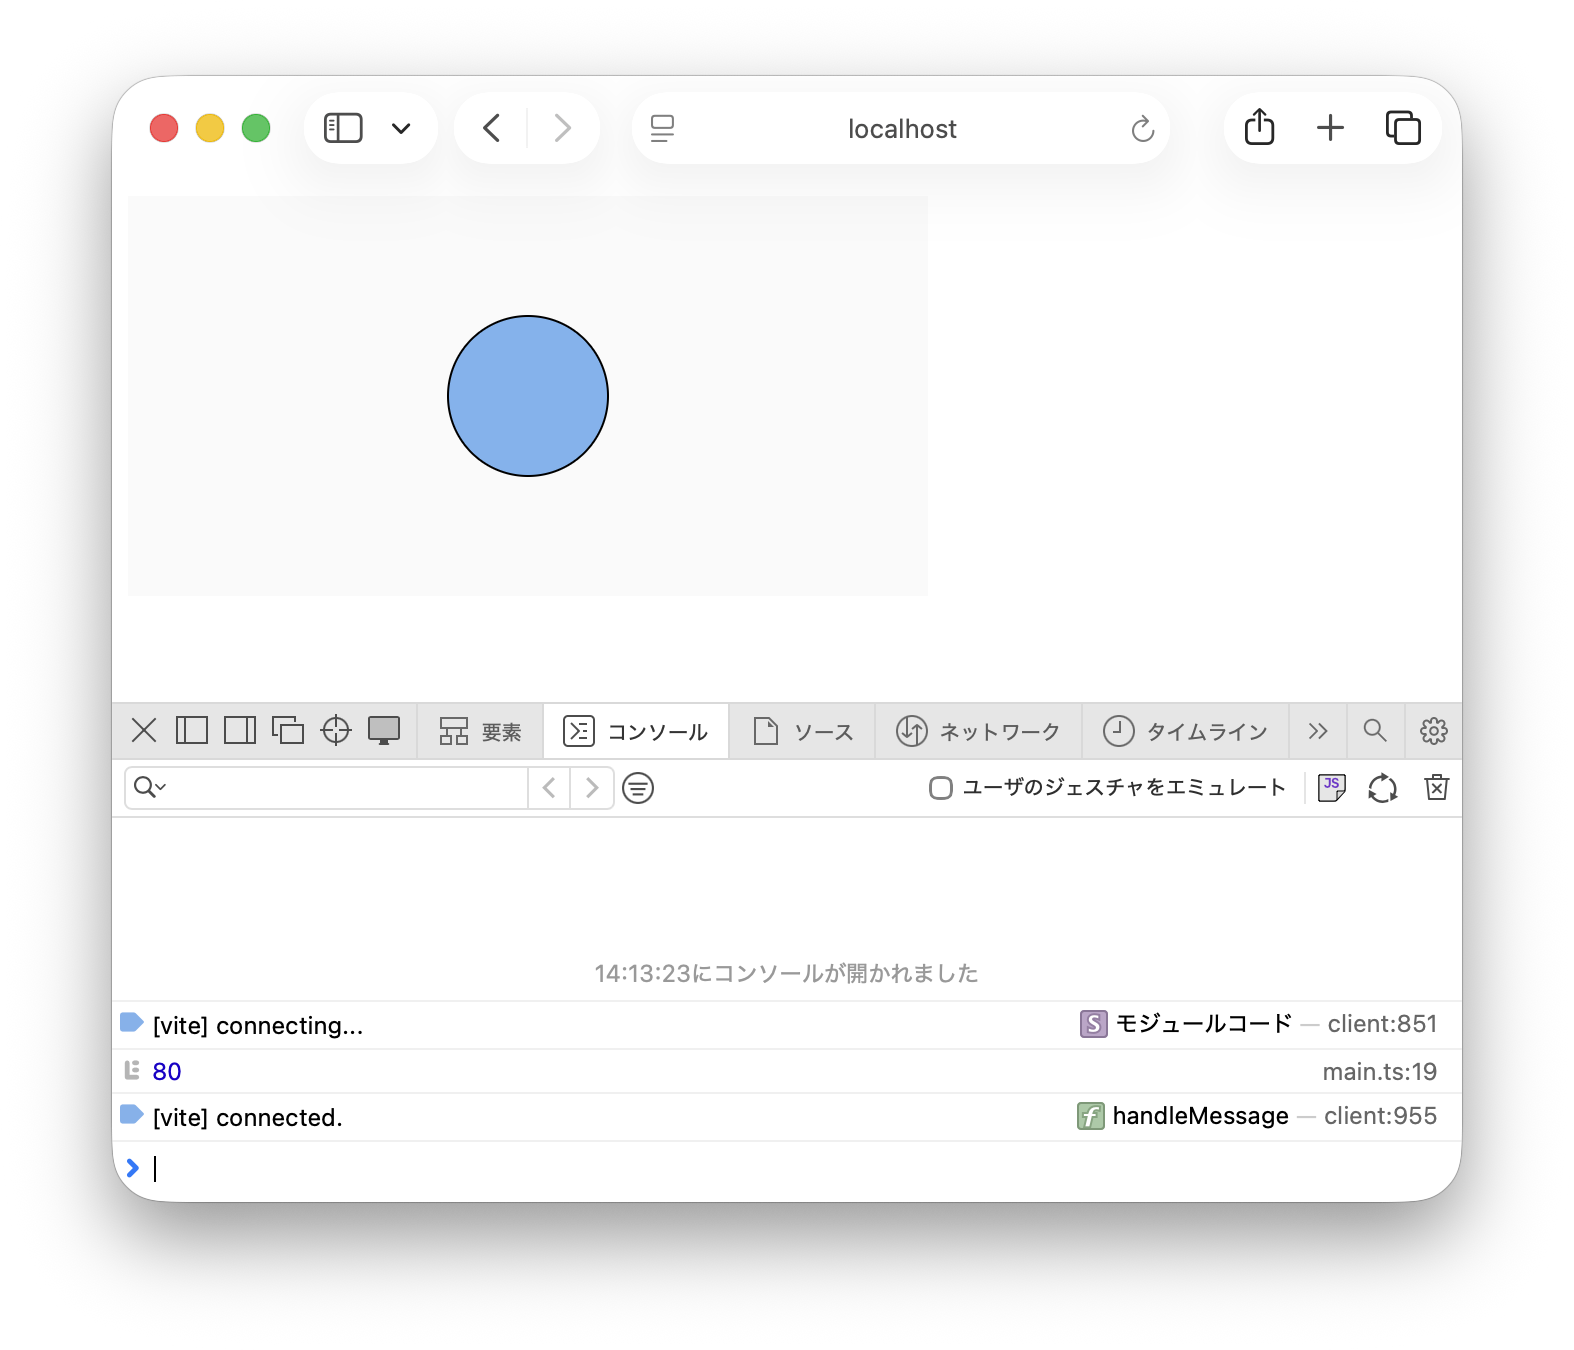
\includegraphics[width=0.6\textwidth]{figures/chapter04/console-value.png}
    \caption{ブラウザの開発者ツールのコンソールに表示された値}
    \label{fig:chapter04-console-value}
\end{figure}

自分の使っているブラウザで、\texttt{console.log}で出力されたものを見る方法を確認しておいて下さい。

\section{円弧を描く}

円や楕円の一部分だけを描きたいときには、\texttt{arc}関数を使います。
\texttt{arc}関数は角度を指定するため、少しだけ新しい考え方が入ります。
ここでは詳しい角度の計算には踏み込まず、口が開いた円のような形を描くための命令として使ってみます。

\begin{listing}[htbp]
\inputminted{ts}{listings/chapter04/arc-pacman.ts}
\caption{arcで口が開いた円を描く}
\label{lst:chapter04-arc-pacman}
\end{listing}

\texttt{p.arc}の最初の4つの数値は、\texttt{p.ellipse}と同じように、中心の位置、幅、高さを表します。その後ろに、描き始める角度と描き終わる角度を指定します。このサンプルでは、\texttt{startAngle}と\texttt{endAngle}という変数を使い、どの角度からどの角度まで描くのかを読み取りやすくしています。最後の\texttt{p.PIE}は、円弧の両端を中心と結び、扇形のように描くための指定です。

\begin{figure}[htbp]
    \centering
    \begin{tikzpicture}[x=1cm, y=-1cm, font=\small]
        \tikzset{
            guide/.style={draw=black!35, dashed, line width=0.6pt},
            arrow/.style={->, line width=0.7pt},
            measure/.style={<->, line width=0.7pt},
            arcline/.style={draw=orange!80!black, fill=yellow!60, line width=1pt},
            labelbox/.style={
                draw=black!35,
                fill=white,
                rounded corners=2pt,
                inner xsep=5pt,
                inner ysep=3pt,
                align=center
            }
        }

        \coordinate (center) at (0,0);
        \coordinate (start) at ({2.5*cos(45)},{1.5*sin(45)});
        \coordinate (end) at ({2.5*cos(315)},{1.5*sin(315)});

        \draw[guide] (-2.5,-1.5) rectangle (2.5,1.5);
        \draw[guide] (center) ellipse (2.5 and 1.5);
        \path[arcline]
            (start)
            plot[domain=45:315, samples=90]
                ({2.5*cos(\x)}, {1.5*sin(\x)})
            -- (center) -- cycle;
        \fill (center) circle (2pt);
        \node[labelbox, anchor=west] at (0.25,0.15) {中心\\\texttt{(x, y)}};

        \draw[measure] (-2.5,2.05) -- node[below] {\texttt{w}} (2.5,2.05);
        \draw[measure] (-3.05,-1.5) -- node[left] {\texttt{h}} (-3.05,1.5);

        \draw[arrow, red!70!black] (center) -- (start);
        \draw[arrow, blue!70!black] (center) -- (end);
        \node[labelbox, anchor=west] at (2.0,1.1) {\texttt{startAngle}\\\texttt{p.QUARTER\_PI}};
        \node[labelbox, anchor=west] at (2.0,-1.1) {\texttt{endAngle}\\\texttt{p.TWO\_PI - p.QUARTER\_PI}};

        \draw[arrow] (3.7,0) arc[start angle=0, end angle=70, radius=0.7];
        \node[anchor=west, align=left] at (4.0,0.9) {角度は右向きから\\時計回りに増える};

        \node[align=center, font=\ttfamily\small] at (0,2.9)
            {p.arc(x, y, w, h, startAngle, endAngle, p.PIE)};
    \end{tikzpicture}
    \caption{\texttt{arc}関数の引数と円弧の関係}
    \label{fig:chapter04-arc-arguments}
\end{figure}

p5.jsでは、標準では角度をラジアンという単位で表します。
学校でよく使う90度、180度、360度のような表し方とは違いますが、
円を一周する角度を\texttt{p.TWO\_PI}$=2\pi$と考えると、最初は扱いやすくなります。
p5.jsの画面では、右向きが\texttt{0}で、そこから時計回りに角度が増えていきます。
そのため、下向きが\texttt{p.HALF\_PI}$=\frac{\pi}{2}$、
左向きが\texttt{p.PI}$=\pi$、
一周して右向きに戻る角度が\texttt{p.TWO\_PI}$=2\pi$になります（図\ref{fig:chapter04-p5-angle-directions}参照）。

\begin{figure}[htbp]
    \centering
    \begin{tikzpicture}[x=1cm, y=-1cm, font=\small]
        \tikzset{
            axis/.style={->, draw=black!45, line width=0.7pt},
            guide/.style={draw=black!30, dashed, line width=0.5pt},
            anglearrow/.style={->, draw=orange!80!black, line width=1.2pt},
            pointlabel/.style={
                draw=black!35,
                fill=white,
                rounded corners=2pt,
                inner xsep=5pt,
                inner ysep=3pt,
                align=center
            }
        }

        \coordinate (center) at (0,0);
        \draw[guide] (center) circle (2.0);
        \draw[axis] (-2.55,0) -- (2.8,0) node[right] {$x$};
        \draw[axis] (0,-2.55) -- (0,2.8) node[below] {$y$};
        \fill (center) circle (2pt);

        \draw[anglearrow]
            (1.05,0)
            arc[start angle=0, end angle=90, radius=1.05];
        \node[align=center] at (1.65,0.75) {角度は\\時計回り};

        \fill (2.0,0) circle (2pt);
        \fill (0,2.0) circle (2pt);
        \fill (-2.0,0) circle (2pt);
        \fill (0,-2.0) circle (2pt);

        \node[pointlabel, anchor=west] at (2.25,0) {\texttt{0}\\右向き};
        \node[pointlabel, anchor=north] at (0,2.35) {\texttt{p.HALF\_PI}\\下向き};
        \node[pointlabel, anchor=east] at (-2.25,0) {\texttt{p.PI}\\左向き};
        \node[pointlabel, anchor=south] at (0,-2.35) {\texttt{p.PI + p.HALF\_PI}\\上向き};
        \node[pointlabel, anchor=west] at (2.25,1.15) {\texttt{p.TWO\_PI}\\一周して右向き};
    \end{tikzpicture}
    \caption{p5.jsにおける角度の向き}
    \label{fig:chapter04-p5-angle-directions}
\end{figure}

\section{よくある間違い}

変数を使うとプログラムは読みやすくなりますが、名前、型、代入のルールを混同するとエラーや意図しない動作の原因になります。

\begin{mistakebox}{変数名が短すぎて意味が分からない}
\texttt{x}や\texttt{d}だけでは、何を表す値なのか分かりにくいことがあります。短いサンプルでは使える場合もありますが、教材では\texttt{circleX}や\texttt{circleDiameter}のように意味が分かる名前を使います。
\end{mistakebox}

\begin{mistakebox}{同じ名前の変数をもう一度作る}
同じ場所で\texttt{const circleX: number = 100;}と書いた後、もう一度\texttt{const circleX: number = 240;}と書くことはできません。値を変えたい場合は、\texttt{let}で作ってから代入します。
\end{mistakebox}

\begin{mistakebox}{number型に文字列を入れる}
\texttt{const circleX: number = "100";}のように、\texttt{number}型の変数に文字列を入れることはできません。数字として使う値は、引用符で囲まずに書きます。
\end{mistakebox}

\begin{mistakebox}{p.widthのp.を付け忘れる}
instance modeでは、\texttt{width}ではなく\texttt{p.width}と書きます。\texttt{height}、\texttt{mouseX}、\texttt{mouseY}なども同じように\texttt{p.}を付けます。
\end{mistakebox}

\begin{mistakebox}{arcの角度を普通の度数だと思う}
\texttt{p.arc}の角度は、90度や180度のような度数ではなく、ラジアンで指定します。最初は\texttt{p.QUARTER\_PI}、\texttt{p.PI}、\texttt{p.TWO\_PI}のような用意された値を使うと分かりやすいです。
\end{mistakebox}

\section{まとめ}

この章では、変数と型注釈を使って、数値に意味のある名前を付ける方法を学びました。\texttt{const}は変わらない値、\texttt{let}は後から変える値に使います。数値を表す型注釈として、\texttt{: number}を書きます。

また、変数を使って計算式を書いたり、\texttt{p.width}や\texttt{p.height}からキャンバスの大きさを利用したりする方法も確認しました。最後に、\texttt{p.arc}で円の一部を描き、角度にも名前を付けられることを見ました。変数を使う目的は、単に短く書くことではなく、プログラムの意味を読みやすくすることです。

\section{演習問題}

この章の演習では、直接書いていた数値を変数に置き換えながら、型注釈と変数名の付け方に慣れていきます。最初はサンプルの一部を変更し、最後は自分の図形作品を変数で整理してみましょう。

\begin{enumerate}
    \item \texttt{circleDiameter}の値を変えて、3つの円の大きさをまとめて変えてください。
    \item \texttt{circleY}の値を変えて、3つの円を上や下に移動してください。
    \item \texttt{const}で背景の明るさを表す\texttt{backgroundGray}を作り、\texttt{p.background}で使ってください。
    \item \texttt{let circleX: number}を使い、同じ変数の値を変えながら4つの円を横に並べてください。
    \item \texttt{circleSpacing}の値を変えて、円どうしの間隔を広くしたり狭くしたりしてください。
    \item \texttt{p.width / 2}と\texttt{p.height / 2}を使い、キャンバスの中央に長方形を描いてください。
    \item \texttt{circleRadius}から\texttt{circleDiameter}を計算し、その直径で円を描いてください。
    \item 第3章で作った色付きの顔のサンプル\ref{lst:chapter03-color-state}で、顔の中心座標や目の直径を変数にしてください。
    \item \texttt{console.log}を使い、計算した直径や中央座標の値を確認してください。
    \item \texttt{p.arc}を使い、口の開き方が違う円を2つ描いてください。
    \item 挑戦問題として、家、ロボット、パックマン風のキャラクターなどを作り、位置、大きさ、色、角度の数値を分かりやすい変数名で整理してください。
\end{enumerate}

\chapter{アニメーションの基本}
\label{chap:animation-basics}

この章では、図形を少しずつ動かしてアニメーションを作る方法を学びます。これまでの章では、1枚の静止した絵を描くことが中心でした。ここからは、\texttt{draw}が繰り返し実行される仕組みを使い、変数の値を少しずつ変えながら動きを作ります。

\section{この章の概要}

アニメーションは、少しずつ違う絵を連続して表示することで作られます。p5.jsでは、\texttt{draw}関数に書いた処理が何度も実行されます。
そのたびに位置を表す変数を少し変えると、図形が動いて見えます。

この章で扱う主な内容は次の通りです。

\begin{itemize}
    \item \texttt{setup}と\texttt{draw}の役割
    \item 位置を表す変数を少しずつ変える方法
    \item 速度を変数として扱う方法
    \item \texttt{background}を書く位置による見え方の違い
    \item \texttt{p.frameCount}によるフレーム数の利用
    \item 第4章の\texttt{arc}を動かす例
\end{itemize}

\section{setupとdraw}

p5.jsでは、\texttt{setup}関数に書いた処理は最初に一度だけ実行されます。
一方、\texttt{draw}関数に書いた処理は、プログラムが動いている間、何度も繰り返し実行されます\footnote{通常、\texttt{draw}関数は、1秒間に60回程度実行されます}。
instance modeでは、\texttt{p.setup = (): void => \{ ... \};}と\texttt{p.draw = (): void => \{ ... \};}の形で、p5.jsが実行する関数を登録します。

\begin{figure}[htbp]
    \centering
    \begin{tikzpicture}[x=1cm, y=1cm, font=\small]
        \tikzset{
            startstop/.style={
                draw=black!60,
                fill=gray!10,
                rounded corners=8pt,
                minimum width=3.2cm,
                minimum height=0.8cm,
                align=center
            },
            process/.style={
                draw=black!60,
                fill=blue!8,
                rounded corners=2pt,
                minimum width=4.0cm,
                minimum height=0.9cm,
                align=center
            },
            repeatprocess/.style={
                draw=black!60,
                fill=orange!12,
                rounded corners=2pt,
                minimum width=4.0cm,
                minimum height=0.9cm,
                align=center
            },
            arrow/.style={->, line width=0.8pt, draw=black!70},
            looparrow/.style={->, line width=0.8pt, draw=orange!80!black}
        }

        \node[startstop] (start) at (0, 0) {プログラム開始};
        \node[process] (setup) at (0, -1.5) {\texttt{p.setup}\\最初に1回だけ実行};
        \node[repeatprocess] (draw) at (0, -3.0) {\texttt{p.draw}\\何度も繰り返し実行};
        \node[process] (frame) at (0, -4.5) {画面に1枚の絵を表示\\次のフレームへ};

        \draw[arrow] (start) -- (setup);
        \draw[arrow] (setup) -- (draw);
        \draw[arrow] (draw) -- (frame);
        \draw[looparrow]
            (frame.east) -- (3.0, -4.5) -- (3.0, -3.0) -- (draw.east);

        \node[align=left, anchor=west] at (3.25, -3.75)
            {\texttt{draw}の中では\\位置や色などを\\少しずつ変えられる};
    \end{tikzpicture}
    \caption{\texttt{setup}と\texttt{draw}が実行される流れ}
    \label{fig:chapter05-setup-draw-flow}
\end{figure}

\begin{listing}[htbp]
\inputminted{ts}{listings/chapter05/setup-draw-basic.ts}
\caption{setupとdrawを使った基本形}
\label{lst:chapter05-setup-draw-basic}
\end{listing}

このサンプルでは、円の位置は変わりません。それでも\texttt{draw}関数の中身は繰り返し実行されています。今は同じ絵を何度も描いているため、静止して見えます。

\section{位置を少しずつ変える}

図形を動かすには、位置を表す変数を用意し、\texttt{draw}が実行されるたびにその値を少しずつ変えます。右に動かしたい場合は、$x$ 座標を少しずつ大きくします。

\begin{listing}[htbp]
\inputminted{ts}{listings/chapter05/moving-circle.ts}
\caption{x座標を変えて円を動かす}
\label{lst:chapter05-moving-circle}
\end{listing}

\texttt{circleX}は円の中心の $x$ 座標です。\texttt{circleSpeed}は、1回の\texttt{draw}でどれだけ右に進むかを表しています。
\[
\texttt{circleX} = \texttt{circleX} + \texttt{circleSpeed};
\]
によって、円の位置が少しずつ右へ移動します。

\begin{figure}[htbp]
    \centering
    \begin{tikzpicture}[font=\small]
        \foreach \start/\position/\value/\frameNumber in {
            0/0.65/60/1,
            3.45/0.95/62/2,
            6.90/1.25/64/3,
            10.35/1.55/66/4
        } {
            \draw[thick, fill=gray!6]
                (\start,0) rectangle +(2.65,-1.8);
            \filldraw[fill=orange!45, draw=black]
                (\start+\position,-0.9) circle (0.28);
            \node[align=center] at (\start+1.325,-2.25)
                {\frameNumber 回目の\texttt{draw}\\
                 \texttt{circleX = \value}};
        }

        \draw[->, thick] (2.72,-0.9) -- (3.35,-0.9)
            node[midway, above, font=\scriptsize]{\texttt{+2}};
        \draw[->, thick] (6.17,-0.9) -- (6.80,-0.9)
            node[midway, above, font=\scriptsize]{\texttt{+2}};
        \draw[->, thick] (9.62,-0.9) -- (10.25,-0.9)
            node[midway, above, font=\scriptsize]{\texttt{+2}};
    \end{tikzpicture}
    \caption{\texttt{draw}のたびにx座標が変わって円が移動する様子}
    \label{fig:chapter05-circle-frame-sequence}
\end{figure}

図\ref{fig:chapter05-circle-frame-sequence}では、4回の\texttt{draw}を別々の絵として並べています。サンプルと同じように、\texttt{circleX}へ毎回\texttt{2}を加えています。図では変化を見分けやすくするため、円の移動距離を実際の比率より大きく表しています。実際のブラウザでは、この描画が短い間隔で続けて表示されるため、円がなめらかに右へ動いているように見えます。

\begin{pointbox}{動きの基本}
アニメーションの基本は、「描く」「値を変える」を繰り返すことです。位置を変えれば移動し、大きさを変えれば拡大や縮小のように見えます。
\end{pointbox}

\section{実数の速度を使う}

速度の値を小さくすると、動きはゆっくりになります。TypeScriptの\texttt{number}型には\texttt{2}と\texttt{0.5}のどちらも保存できるため、\texttt{0.8}のような値を速度として使うことができます。

\begin{listing}[htbp]
\inputminted{ts}{listings/chapter05/fractional-speed.ts}
\caption{小数の速度で円をゆっくり動かす}
\label{lst:chapter05-fractional-speed}
\end{listing}

このサンプルでは、\texttt{circleY}を少しずつ大きくしています。p5.jsでは下に進むほど $y$ 座標が大きくなるため、円は下へ移動します。

\section{backgroundをdrawに書く}

アニメーションでは、前のフレームに描いた図形を消してから、新しい位置に図形を描くことがよくあります。そのためには、\texttt{background}関数を\texttt{draw}関数の中に書きます。

\begin{listing}[htbp]
\inputminted{ts}{listings/chapter05/background-in-draw.ts}
\caption{drawの中で背景を塗り直す}
\label{lst:chapter05-background-in-draw}
\end{listing}

このサンプルでは、毎回\texttt{p.background(245)}で画面全体を塗り直してから円を描いています。そのため、前の位置の円は残らず、1つの円が動いているように見えます。

\section{backgroundをsetupに書く}

\texttt{background}関数を\texttt{setup}関数にだけ書くと、背景は最初に一度だけ塗られます。その後の\texttt{draw}では前の図形が消されないため、動いた跡が残ります。

\begin{listing}[htbp]
\inputminted{ts}{listings/chapter05/background-in-setup.ts}
\caption{setupだけで背景を塗る}
\label{lst:chapter05-background-in-setup}
\end{listing}

このサンプルでは、円が移動した場所が画面に残ります。これは間違いとは限りません。軌跡を描きたいときには便利です。ただし、1つの物体だけが動いているように見せたい場合は、\texttt{background}を\texttt{draw}の中に書きます。

\begin{figure}[htbp]
    \centering
    \begin{minipage}[t]{0.47\linewidth}
        \centering
        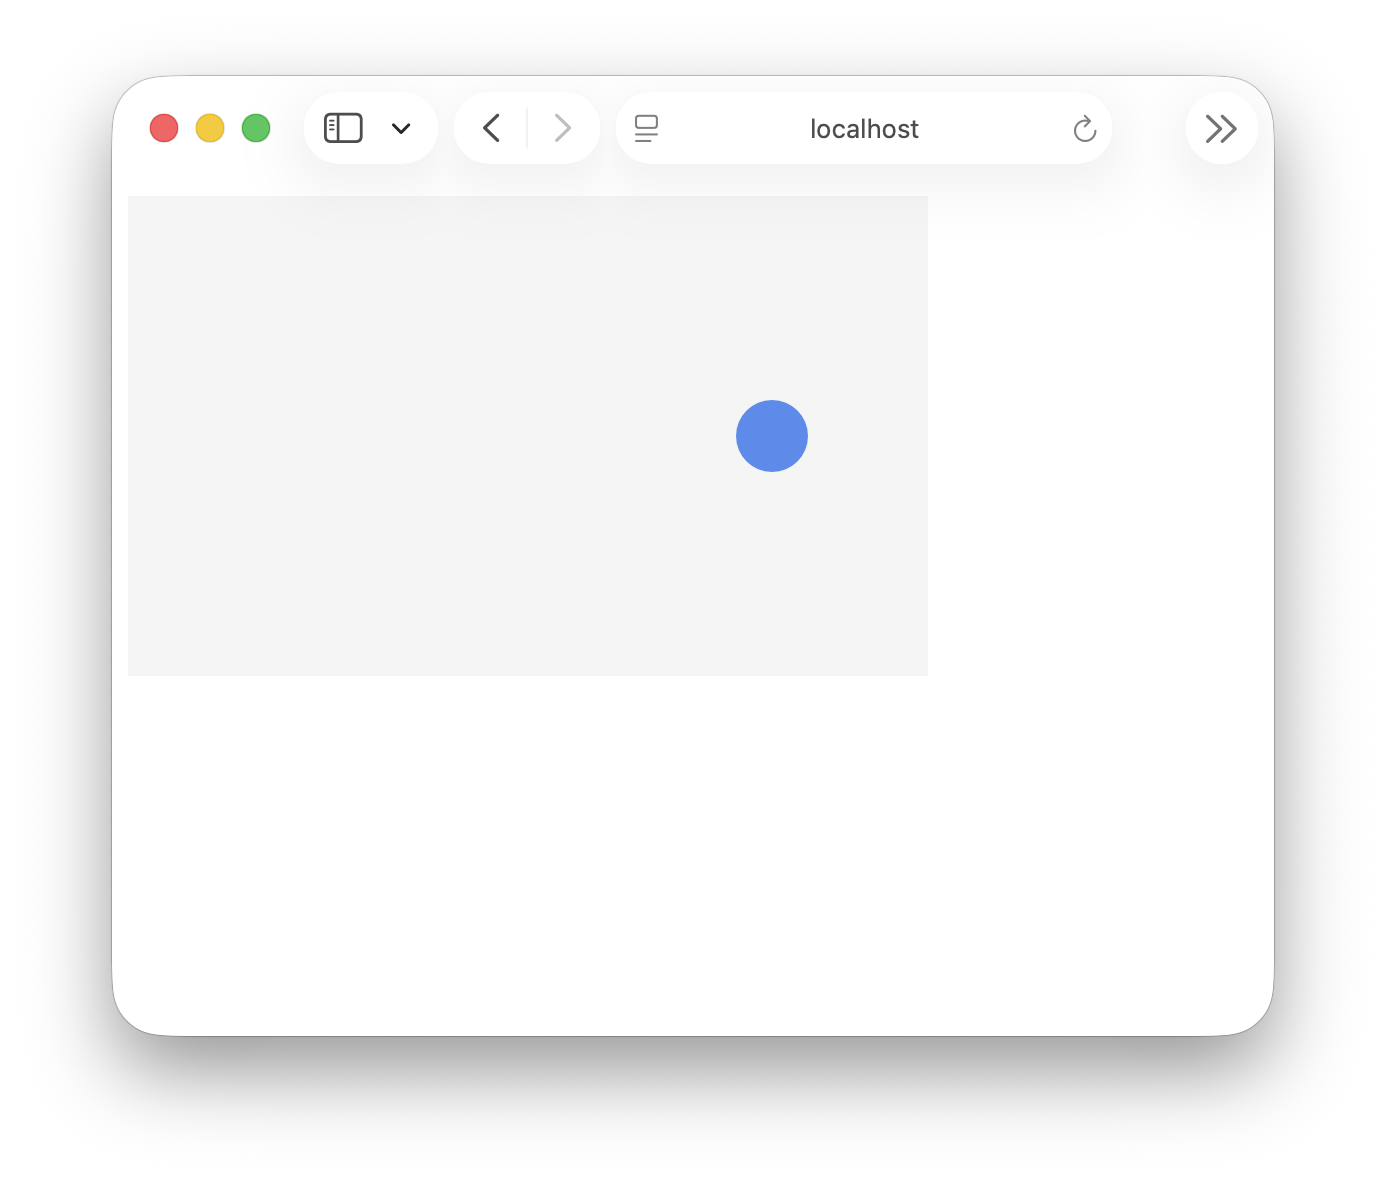
\includegraphics[
            width=\linewidth,
            trim=50 212 193 35,
            clip
        ]{figures/chapter05/background-in-draw.png}

        \small \texttt{draw}で\texttt{background}を実行
    \end{minipage}
    \hfill
    \begin{minipage}[t]{0.47\linewidth}
        \centering
        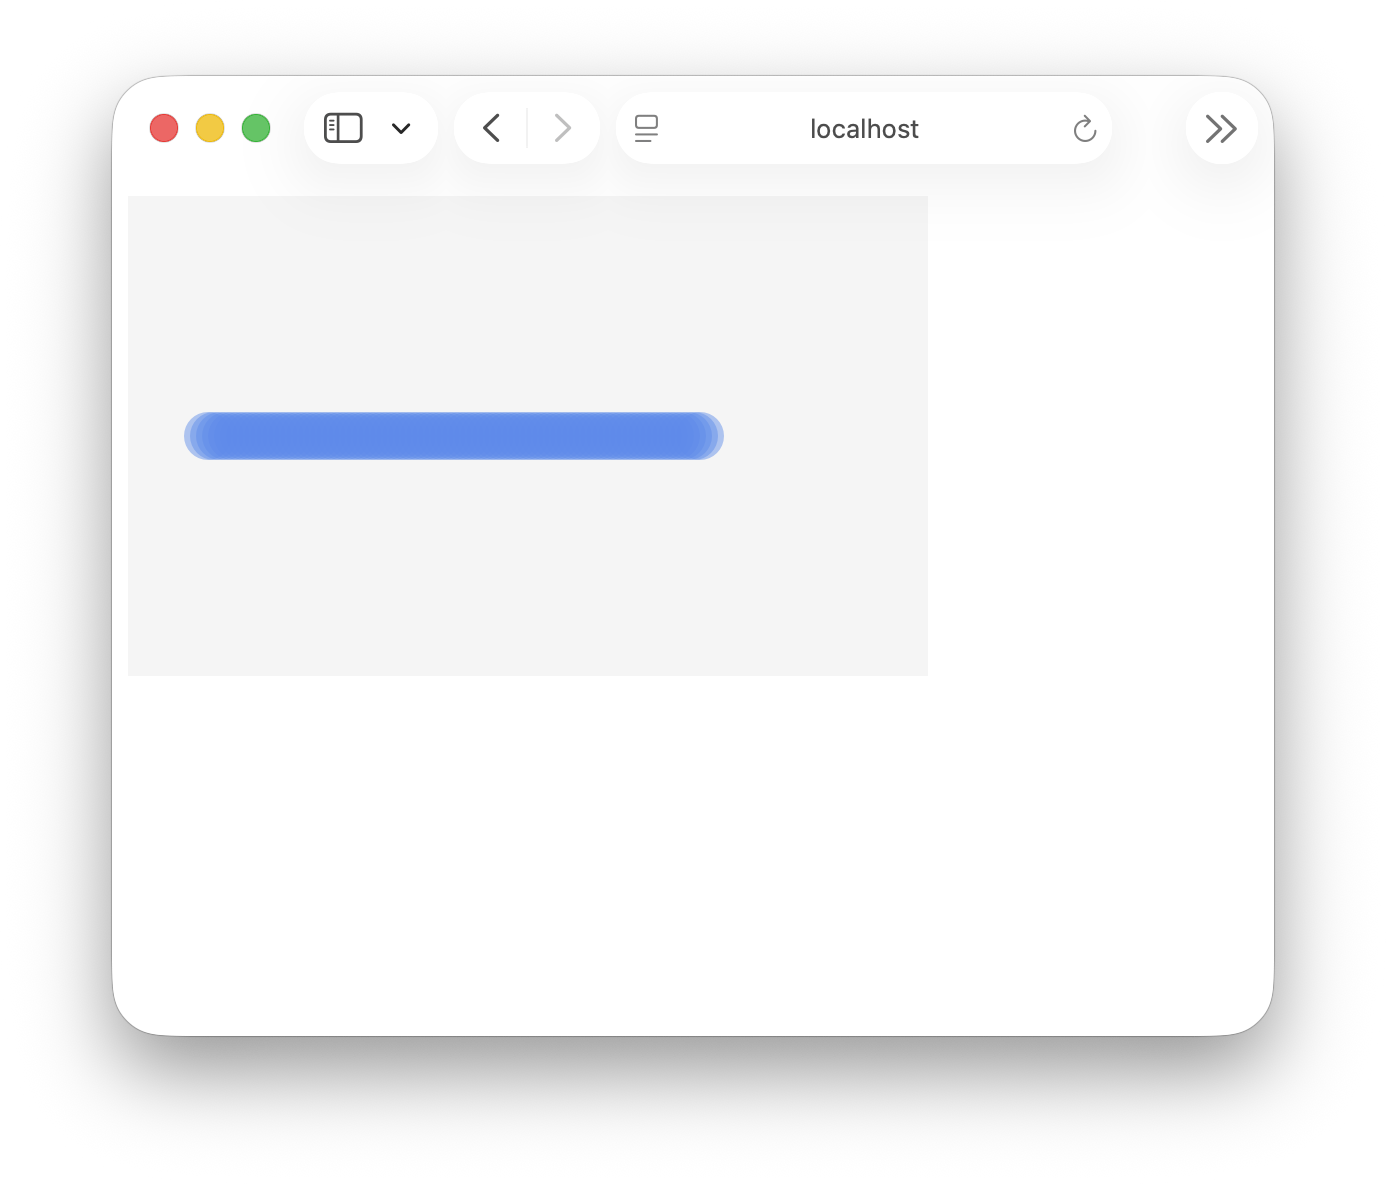
\includegraphics[
            width=\linewidth,
            trim=50 212 193 35,
            clip
        ]{figures/chapter05/background-in-setup.png}

        \small \texttt{setup}で最初にだけ\texttt{background}を実行
    \end{minipage}
    \caption{\texttt{background}を書く場所による実行画面の違い}
    \label{fig:chapter05-background-placement-results}
\end{figure}

図\ref{fig:chapter05-background-placement-results}の左側では、\texttt{draw}のたびに背景を塗り直すため、現在の位置にある円だけが見えます。右側では、背景を最初に一度しか塗らないため、それまでに描かれた円が軌跡として残ります。

\begin{notebox}{backgroundの場所}
\texttt{background}を\texttt{draw}に書くと毎回画面を消します。\texttt{setup}にだけ書くと、前に描いた図形が残ります。どちらが正しいかではなく、作りたい見た目に合わせて選びます。
\end{notebox}

\section{\texttt{frameCount}を使う}

p5.jsには、システム変数\texttt{frameCount}が用意されています。
これは、\texttt{draw}が何回実行されたかを表す数値です。
毎回少しずつ増える値として使うことができます。
コード上では、\texttt{p.frameCount}のように、スケッチを表す変数を通して使います。

\begin{listing}[htbp]
\inputminted{ts}{listings/chapter05/frame-count.ts}
\caption{frameCountで大きさを変える}
\label{lst:chapter05-frame-count}
\end{listing}

このサンプルでは、\texttt{frameCount}変数を使って円の直径を計算しています。時間が進むにつれて\texttt{frameCount}変数の値が大きくなるため、円も少しずつ大きくなります。

\begin{notebox}{frameCountは読み取る値}
\texttt{frameCount}変数はp5.jsが用意している値です。自分で代入して変更するものではなく、現在のフレーム数を読み取るために使います。
\end{notebox}

\section{arcを動かす}

第4章では、\texttt{arc}関数を使って口が開いた円を描きました(サンプル\ref{lst:chapter04-arc-pacman})。
同じ考え方で、\texttt{arc}の中心座標を少しずつ変えると、パックマン風のキャラクターが移動しているように見せることができます。

\begin{listing}[htbp]
\inputminted[fontsize=\small]{ts}{listings/chapter05/moving-pacman.ts}
\caption{arcで描いたキャラクターを動かす}
\label{lst:chapter05-moving-pacman}
\end{listing}

このサンプルでは、\texttt{characterX}を少しずつ大きくしています。\texttt{arc}関数の中心を表す引数の $x$ 座標に\texttt{characterX}を使っているため、キャラクター全体が右へ移動します。

\begin{pointbox}{p.を付ける理由}
instance modeでは、p5.jsが用意している命令や値を\texttt{p}から使います。そのため、\texttt{background}ではなく\texttt{p.background}、\texttt{frameCount}ではなく\texttt{p.frameCount}と書きます。
\end{pointbox}

\section{よくある間違い}

アニメーションでは、文法は正しくても、変数を更新する場所や背景を塗る場所によって、思った通りに見えないことがあります。

\begin{mistakebox}{位置を表す変数をdrawの中で毎回初期化する}
\texttt{draw}の中で\texttt{let circleX: number = 60;}のように書くと、毎回同じ値から始まってしまいます。動かしたい位置の変数は、\texttt{draw}の外側に用意します。
\end{mistakebox}

\begin{mistakebox}{変数の値を更新していない}
円を描くだけでは位置は変わりません。\texttt{circleX = circleX + circleSpeed;}のように、位置を表す変数を更新する必要があります。
\end{mistakebox}

\begin{mistakebox}{backgroundの場所を間違える}
前の図形を消したいときは、\texttt{p.background}を\texttt{p.draw}の中に書きます。軌跡を残したいときは、\texttt{p.setup}だけに書く方法もあります。
\end{mistakebox}

\begin{mistakebox}{速さを大きくしすぎる}
\texttt{circleSpeed}が大きすぎると、図形が一気に移動して見えます。最初は\texttt{1}から\texttt{3}くらいの値で試すと違いが分かりやすいです。
\end{mistakebox}

\section{まとめ}

この章では、\texttt{setup}と\texttt{draw}を使ってアニメーションを作る基本を学びました。\texttt{setup}は最初に一度だけ実行され、\texttt{draw}は繰り返し実行されます。

また、位置や速度を変数で表し、\texttt{draw}の中で少しずつ値を変えることで動きを作りました。\texttt{background}を書く場所によって、前の絵を消すか、軌跡として残すかが変わることも確認しました。

\section{演習問題}

この章の演習では、円や\texttt{arc}を少しずつ動かしながら、アニメーションの基本を確認します。まずは数値を変えて動きの違いを観察し、最後は自分の動く作品を作ってみましょう。

\begin{enumerate}
    \item \texttt{moving-circle.ts}の\texttt{circleSpeed}を変えて、円の速さを変えてください。
    \item \texttt{circleX}の初期値を変えて、円が動き始める位置を変えてください。
    \item \texttt{circleY}を変化させて、円が下に動くアニメーションを作ってください。
    \item \texttt{circleSpeed}に小数を使い、ゆっくり動く円を作ってください。
    \item \texttt{background}関数を\texttt{draw}から\texttt{setup}へ移動し、見え方の違いを説明してください。
    \item \texttt{background}関数の色を変えて、暗い背景や明るい背景で動きを確認してください。
    \item \texttt{frameCount}変数を使い、時間とともに円が大きくなるサンプルを変更してください。
    \item \texttt{arc}関数で描いたキャラクターの大きさや色を変えてください。
    \item \texttt{characterSpeed}を変えて、パックマン風のキャラクターの移動速度を調整してください。
    \item 挑戦問題として、円、四角形、\texttt{arc}のいずれかを使い、横または縦に動く短いアニメーション作品を作ってください。
\end{enumerate}

\chapter{条件分岐とインタラクション}
\label{chap:conditions-and-interaction}

この章では、条件によって処理を変える方法と、マウスやキーボードからの入力を使ってプログラムを操作する方法を学びます。第5章では、変数の値を毎回少しずつ変えることでアニメーションを作りました。この章では、そこに「もし〜なら」という判断を加え、画面の状態やユーザーの操作に反応するプログラムを作ります。

\section{この章の概要}

条件分岐は、プログラムに判断をさせるための仕組みです。たとえば、「マウスボタンが押されているなら円を黒くする」「円が画面の端に着いたら向きを変える」のように、ある条件が成り立つかどうかで実行する処理を変えます。

この章で扱う主な内容は次の通りです。

\begin{itemize}
    \item 条件式と\texttt{boolean}型
    \item \texttt{if}文と\texttt{if}〜\texttt{else}文
    \item \texttt{if}〜\texttt{else if}〜\texttt{else}文
    \item 比較演算子の使い方
    \item \texttt{p.mouseX}、\texttt{p.mouseY}、\texttt{p.mouseIsPressed}
    \item 壁で跳ね返るアニメーション
    \item \texttt{p.mousePressed}と\texttt{p.keyPressed}
\end{itemize}

\section{条件式とboolean型}

条件分岐では、「正しい」か「正しくない」かを判定する式を使います。このような式を条件式と呼びます。TypeScriptでは、条件式の結果は\texttt{boolean}型の値になります。\texttt{boolean}型の値は、\texttt{true}または\texttt{false}のどちらかです。

\begin{center}
\begin{tabular}{ll}
\toprule
条件式 & 意味 \\
\midrule
\texttt{p.mouseX < 200} & マウスの $x$ 座標が200より小さい \\
\texttt{circleX >= p.width} & 円の $x$ 座標がキャンバスの幅以上 \\
\texttt{p.mouseIsPressed} & マウスボタンが押されている \\
\texttt{p.key === "a"} & 押されたキーが\texttt{a}である \\
\bottomrule
\end{tabular}
\end{center}

\begin{pointbox}{boolean型}
\texttt{boolean}型は、\texttt{true}または\texttt{false}を入れるための型です。条件式も、最終的には\texttt{true}か\texttt{false}のどちらかとして扱われます。
\end{pointbox}

\section{if文で処理を選ぶ}

\texttt{if}文は、条件が成り立つときだけ処理を実行するための書き方です。まずは、マウスボタンが押されているときだけ円の色を変える例を見てみましょう。

\begin{figure}[htbp]
    \centering
    \begin{tikzpicture}[
        font=\small,
        box/.style={draw, rounded corners=2pt, minimum width=35mm, minimum height=8mm, align=center},
        decision/.style={
            draw,
            diamond,
            aspect=2.2,
            minimum width=34mm,
            minimum height=18mm,
            align=center
        }
    ]
        \node[box] (start) at (0, 0) {処理を始める};
        \node[decision] (condition) at (0, -1.8) {\texttt{p.mouseIsPressed}\\は\texttt{true}?};
        \node[box] (then) at (0, -3.7) {\texttt{p.fill(40);}\\を実行する};
        \node[box] (end) at (0, -5.4) {次の処理へ進む};

        \draw[->] (start) -- (condition);
        \draw[->] (condition) -- node[right]{true} (then);
        \draw[->] (then) -- (end);
        \draw[->] (condition.east) -- ++(1.8, 0) node[right]{false} |- (end.east);
    \end{tikzpicture}
    \caption{if文の処理の流れ}
    \label{fig:chapter06-if-flowchart}
\end{figure}

\begin{listing}[htbp]
\inputminted{ts}{listings/chapter06/mouse-pressed-fill.ts}
\caption{マウスボタンが押されているときだけ色を変える}
\label{lst:chapter06-mouse-pressed-fill}
\end{listing}

\texttt{p.mouseIsPressed}は、マウスボタンが押されているときに\texttt{true}、押されていないときに\texttt{false}になる\texttt{boolean}型の値です。このサンプルでは、まず灰色で塗るように指定し、\texttt{true}のときだけ\texttt{p.fill(40);}で黒に近い色へ上書きします。

\begin{notebox}{何もしない場合もある}
\texttt{if}文だけを書くと、条件が成り立たないときは、その中の処理が実行されません。このサンプルでは、マウスを押していないときには\texttt{p.fill(40);}が実行されないため、その直前に指定した灰色で円が描かれます。
\end{notebox}

\section{ifとelseを使う}

条件が成り立つときと、成り立たないときの両方に処理を書きたい場合は、\texttt{if}〜\texttt{else}文を使います。\texttt{else}は「そうでなければ」という意味で読むと理解しやすくなります。

\begin{figure}[htbp]
    \centering
    \begin{tikzpicture}[
        font=\small,
        box/.style={draw, rounded corners=2pt, minimum width=34mm, minimum height=8mm, align=center},
        decision/.style={
            draw,
            diamond,
            aspect=2.2,
            minimum width=34mm,
            minimum height=18mm,
            align=center
        }
    ]
        \node[box] (start) at (0, 0) {処理を始める};
        \node[decision] (condition) at (0, -1.8) {\texttt{p.mouseIsPressed}\\は\texttt{true}?};
        \node[box] (then) at (-2.8, -3.7) {\texttt{p.fill(40);}\\を実行する};
        \node[box] (else) at (2.8, -3.7) {\texttt{p.fill(180);}\\を実行する};
        \node[box] (end) at (0, -5.5) {次の処理へ進む};

        \draw[->] (start) -- (condition);
        \draw[->] (condition) -| node[pos=.25, above]{true} (then);
        \draw[->] (condition) -| node[pos=.25, above]{false} (else);
        \draw[->] (then) |- (end);
        \draw[->] (else) |- (end);
    \end{tikzpicture}
    \caption{if〜else文の処理の流れ}
    \label{fig:chapter06-if-else-flowchart}
\end{figure}

\begin{listing}[htbp]
\inputminted{ts}{listings/chapter06/mouse-pressed-if-else.ts}
\caption{ifとelseで円の色を切り替える}
\label{lst:chapter06-mouse-pressed-if-else}
\end{listing}

このサンプルでは、マウスボタンが押されているときは黒に近い色、押されていないときは灰色で円を描きます。どちらの場合にも必ず\texttt{p.fill}が実行されるため、状態の違いがはっきりします。

\section{if、else if、elseを使う}

選びたい処理が3つ以上ある場合は、\texttt{if}、\texttt{else if}、\texttt{else}を組み合わせます。最初の条件から順番に調べ、成り立ったところの処理だけを実行します。

\begin{figure}[htbp]
    \centering
    \begin{tikzpicture}[
        font=\small,
        box/.style={draw, rounded corners=2pt, minimum width=32mm, minimum height=8mm, align=center},
        decision/.style={
            draw,
            diamond,
            aspect=2.2,
            minimum width=34mm,
            minimum height=18mm,
            align=center
        }
    ]
        \node[box] (start) at (0, 0) {処理を始める};
        \node[decision] (conditionA) at (0, -1.9) {条件1は\\\texttt{true}?};
        \node[box] (thenA) at (-4.3, -1.9) {処理1を\\実行する};
        \node[decision] (conditionB) at (0, -4.5) {条件2は\\\texttt{true}?};
        \node[box] (thenB) at (4.3, -4.5) {処理2を\\実行する};
        \node[box] (else) at (0, -6.9) {それ以外の\\処理を実行する};
        \node[box] (end) at (0, -8.7) {次の処理へ進む};

        \draw[->] (start) -- (conditionA);
        \draw[->] (conditionA) -- node[above]{true} (thenA);
        \draw[->] (conditionA) -- node[right]{false} (conditionB);
        \draw[->] (conditionB) -- node[above]{true} (thenB);
        \draw[->] (conditionB) -- node[right]{false} (else);
        \draw[->] (thenA) |- (end);
        \draw[->] (thenB) |- (end);
        \draw[->] (else) -- (end);
    \end{tikzpicture}
    \caption{if〜else if〜else文の処理の流れ}
    \label{fig:chapter06-if-else-if-flowchart}
\end{figure}

\begin{listing}[htbp]
\inputminted{ts}{listings/chapter06/mouse-third-rect.ts}
\caption{if〜else if〜elseで3つの領域を塗り分ける}
\label{lst:chapter06-mouse-third-rect}
\end{listing}

このサンプル（リスト\ref{lst:chapter06-mouse-third-rect}）では、キャンバスを左、中央、右の3つの領域に分けています。マウスが左の領域にあれば最初の\texttt{if}の処理を実行します。左ではなく中央にあれば\texttt{else if}の処理を実行します。どちらでもなければ、右の領域にあると考えて\texttt{else}の処理を実行します。

\begin{pointbox}{上から順番に調べる}
\texttt{else if}は、前の条件が成り立たなかったときだけ調べられます。複数の条件を並べるときは、どの順番で調べると分かりやすいかを考えます。
\end{pointbox}

\section{マウスの位置で処理を変える}

マウスの位置を使うと、画面のどこにカーソルがあるかによって表示を変えられます。p5.jsでは、マウスカーソルの $x$ 座標をシステム変数\texttt{mouseX}、$y$ 座標を\texttt{mouseY}として読み取ります。
\footnote{\texttt{frameCount}と同じように、プログラム内では、\texttt{p.mouseX}、\texttt{p.mouseY}のように、スケッチを表す変数を通して使います。}

\begin{listing}[htbp]
\inputminted{ts}{listings/chapter06/mouse-half-rect.ts}
\caption{マウスの位置で左右の領域を塗り分ける}
\label{lst:chapter06-mouse-half-rect}
\end{listing}

\texttt{p.mouseX < p.width / 2}は、「マウスがキャンバスの左半分にあるか」を調べる条件式です。左半分にあるときは左側を青く塗り、そうでないときは右側をオレンジ色に塗ります。

\begin{pointbox}{比較演算子}
\texttt{<}、\texttt{>}、\texttt{<=}、\texttt{>=}は数値を比べるための演算子です。\texttt{=}は代入に使うため、「等しい」を調べるときは\texttt{===}を使います。
\end{pointbox}

\section{端に着いたら向きを変える}

条件分岐は、アニメーションにも使えます。第5章では円が右へ動き続けるだけでした。この章では、円が画面の端に着いたときに移動方向を変え、左右の壁で跳ね返るようにします。

\begin{listing}[htbp]
\inputminted{ts}{listings/chapter06/bouncing-circle.ts}
\caption{画面の端で円を跳ね返す}
\label{lst:chapter06-bouncing-circle}
\end{listing}

\begin{figure}[htbp]
    \centering
    \begin{tikzpicture}[x=0.9cm, y=0.9cm, font=\small]
        \tikzset{
            guide/.style={draw=black!35, dashed},
            measure/.style={<->, line width=0.7pt},
            arrow/.style={->, line width=0.7pt},
            labelbox/.style={
                draw=black!35,
                fill=white,
                rounded corners=2pt,
                inner xsep=5pt,
                inner ysep=3pt,
                align=center
            }
        }

        \draw[fill=blue!4, draw=black!60] (0, 0) rectangle (8, 3);
        \node[anchor=north west] at (0, 3) {キャンバス};

        \coordinate (center) at (6.8, 1.5);
        \coordinate (rightEdge) at (8, 1.5);
        \draw[fill=orange!35, draw=orange!80!black, line width=1pt]
            (center) circle (1.2);
        \fill (center) circle (2pt);
        \draw[guide] (center) -- (6.8, -0.35);
        \draw[guide, red!70!black] (8, 0) -- (8, 3);

        \draw[measure] (center) -- node[above] {\texttt{circleRadius}} (rightEdge);
        \draw[measure] (0, -0.45) -- node[below] {\texttt{p.width}} (8, -0.45);
        \draw[arrow] (6.8, -0.25) -- (6.8, 0);
        \node[labelbox, anchor=south] at (6.8, -0.35) {\texttt{circleX}};
        \node[labelbox, anchor=west] at (8.15, 1.5) {キャンバスの右端};

        \node[labelbox, anchor=north] at (4, -1.0)
            {\texttt{circleX + circleRadius >= p.width}\\なら右端に届いている};
    \end{tikzpicture}
    \caption{円の右端がキャンバスの右端に届く条件}
    \label{fig:chapter06-right-edge-condition}
\end{figure}

\texttt{circleX + circleRadius >= p.width}は、円の右端がキャンバスの右端に届いたかを調べています。右端に届いたら\texttt{circleSpeed}を負の値にして、左向きに動くようにします。反対に、\texttt{circleX - circleRadius <= 0}は、円の左端がキャンバスの左端に届いたかを調べています。

\begin{notebox}{中心ではなく端を見る}
円の中心だけで判定すると、円が半分画面の外へ出てから向きが変わります。半径を使って円の右端と左端を調べると、壁に触れたところで向きを変えられます。
\end{notebox}

\section{マウスに追従させる}

インタラクションでは、マウスカーソルの位置そのものを図形の位置として使うこともできます。
次の例では、円がマウスカーソルを追いかけるように見えます。

\begin{listing}[htbp]
\inputminted{ts}{listings/chapter06/mouse-follow.ts}
\caption{マウスの位置に円を描く}
\label{lst:chapter06-mouse-follow}
\end{listing}

\texttt{p.mouseX}と\texttt{p.mouseY}は、\texttt{draw}関数が実行されるたびに現在のマウスカーソル位置として読み取られます。
そのため、円の中心座標にそのまま使うと、円がマウスに合わせて動きます。

\section{クリックで状態を切り替える}

\texttt{p.mouseIsPressed}は、今マウスが押されているかを調べる値でした。一方、\texttt{p.mousePressed = (): void => \{ ... \};}は、マウスを押した瞬間に1回呼ばれるイベント関数です。クリックするたびに状態を切り替えたい場合に便利です。

\begin{listing}[htbp]
\inputminted{ts}{listings/chapter06/mouse-click-toggle.ts}
\caption{クリックするたびに円の色を切り替える}
\label{lst:chapter06-mouse-click-toggle}
\end{listing}

\texttt{isCircleRed}は、円を赤く塗るかどうかを表す\texttt{boolean}型の変数です。\texttt{isCircleRed = !isCircleRed;}は、\texttt{true}なら\texttt{false}に、\texttt{false}なら\texttt{true}に切り替える書き方です。

\begin{pointbox}{状態を変数で覚える}
クリックされたことを画面に残したい場合は、状態を変数に保存します。\texttt{draw}ではその変数を見て描き方を決め、\texttt{p.mousePressed}のイベント関数ではその変数の値を変更します。
\end{pointbox}

\section{キー入力を使う}

キーボード入力も、マウス入力と同じようにインタラクションに使えます。次の例では、\texttt{a}キーで四角形を左へ、\texttt{d}キーで右へ動かします。

\begin{listing}[htbp]
\inputminted{ts}{listings/chapter06/key-pressed-move.ts}
\caption{キー入力で四角形を動かす}
\label{lst:chapter06-key-pressed-move}
\end{listing}

\texttt{p.keyPressed = (): void => \{ ... \};}は、キーが押された瞬間に実行したい処理を登録するイベント関数です。\texttt{p.key === "a"}は、押されたキーが\texttt{a}かどうかを調べる条件式です。文字を比べるときも、等しいかどうかの判定には\texttt{===}を使います。

\begin{notebox}{大文字と小文字}
\texttt{p.key === "a"}は小文字の\texttt{a}を調べています。環境や入力状態によっては、大文字の\texttt{A}とは別の文字として扱われます。最初は小文字で試しましょう。
\end{notebox}

\section{よくある間違い}

条件分岐と入力処理では、記号の違いや、どのタイミングで処理が実行されるかを混同しやすくなります。エラーが出ない場合でも、条件が思った通りに成り立っていないことがあります。

\begin{mistakebox}{等しいか調べるときに=を書く}
\texttt{=}は代入です。条件式で等しいかどうかを調べるときは、\texttt{p.key === "a"}のように\texttt{===}を使います。
\end{mistakebox}

\begin{mistakebox}{p.を付け忘れる}
instance modeでは、\texttt{mouseX}ではなく\texttt{p.mouseX}、\texttt{mouseIsPressed}ではなく\texttt{p.mouseIsPressed}と書きます。
\end{mistakebox}

\begin{mistakebox}{条件の中で毎回変数を作ってしまう}
クリック後も覚えておきたい値は、\texttt{draw}関数や\texttt{mousePressed}関数の外側に用意します。
関数の中で毎回\texttt{let isCircleRed: boolean = false;}と書くと、
この関数の外側では、変数\texttt{isCircleRed}にアクセスすることができません。
この例のように、外側で\texttt{let isCircleRed: boolean = false;}と宣言しておき、\texttt{mousePressed}関数の中では
\texttt{isCircleRed = !isCircleRed;}のように値を切り替えるだけにします。
\end{mistakebox}

\begin{mistakebox}{境界判定で半径を忘れる}
円が壁に当たったかを調べるときは、中心座標だけでなく半径も使います。\texttt{circleX + circleRadius}と\texttt{circleX - circleRadius}を見ると、円の端で判定できます。
\end{mistakebox}

\section{まとめ}

この章では、条件式、\texttt{boolean}型、\texttt{if}文、\texttt{if}〜\texttt{else}文を使って、処理を選ぶ方法を学びました。条件式は\texttt{true}または\texttt{false}になり、その結果によって実行される処理が変わります。

また、\texttt{p.mouseX}、\texttt{p.mouseY}、\texttt{p.mouseIsPressed}、\texttt{p.mousePressed}、\texttt{p.keyPressed}を使い、ユーザーの操作に反応するプログラムを作りました。条件分岐と入力を組み合わせると、アニメーションは単に動くだけでなく、操作できるものになります。

\section{演習問題}

この章の演習では、条件分岐と入力を使って、画面の変化を自分で制御します。まずは条件式の数値や色を変えるところから始め、最後は小さな操作できる作品に挑戦しましょう。

\begin{enumerate}
    \item \texttt{mouse-pressed-if-else.ts}の色を変えて、押しているときと押していないときの違いを分かりやすくしてください。
    \item \texttt{p.mouseX < p.width / 2}の条件を、\texttt{p.mouseY < p.height / 2}に変えると何が起こるか確認してください。
    \item \texttt{mouse-half-rect.ts}で、左右ではなく上下の領域を塗り分けてください。
    \item \texttt{mouse-third-rect.ts}で、3つの領域の色や幅を変えてください。
    \item \texttt{bouncing-circle.ts}の\texttt{circleSpeed}を変えて、跳ね返る速さを調整してください。
    \item 円が左右ではなく上下に跳ね返るように、\texttt{circleY}と縦方向の速度を使ったプログラムを作ってください。
    \item \texttt{mouse-follow.ts}で、マウスについてくる図形を円から四角形に変えてください。
    \item \texttt{mouse-click-toggle.ts}で、クリックするたびに円の大きさが切り替わるようにしてください。
    \item \texttt{key-pressed-move.ts}に\texttt{w}キーと\texttt{s}キーを追加し、四角形を上下にも動かせるようにしてください。
    \item 四角形が画面の外へ出ないように、端に着いたらそれ以上動かない条件を追加してください。
    \item 挑戦問題として、マウスまたはキーボードで操作できる小さなキャラクターを作り、押すキーやクリックによって色や位置が変わる作品にしてください。
\end{enumerate}

\chapter{繰り返し処理}
\label{chap:loops}

この章では、同じ処理を何度も実行するための繰り返し処理を学びます。第6章では条件によって処理を選びました。この章では、図形をたくさん並べたり、同じ規則で位置を変えたりするために、\texttt{for}文と\texttt{while}文を使います。

\section{この章の概要}

繰り返し処理を使うと、似た命令を何度も書かずに、短く読みやすいプログラムにできます。図形を規則的に並べる、ランダムな位置にたくさん描く、マウスの位置から画面の端まで描く、というような処理でよく使います。

この章で扱う主な内容は次の通りです。

\begin{itemize}
    \item 繰り返し処理が必要になる場面
    \item \texttt{for}文の基本形
    \item カウンタ変数の使い方
    \item \texttt{p.random}を使った繰り返し描画
    \item 繰り返し処理の入れ子
    \item \texttt{while}文の基本形
    \item \texttt{while}文の初期化、条件、更新
    \item 乱数と繰り返しを組み合わせる方法
\end{itemize}

\section{繰り返し処理が必要になる場面}

同じような線を何本も描きたい場合、これまでの知識だけでもプログラムを書くことはできます。ただし、線の本数が増えるほど、同じような命令を何度も書くことになります。

\begin{listing}[htbp]
\inputminted{ts}{listings/chapter07/repeated-lines-without-loop.ts}
\caption{繰り返し処理を使わずに線を並べる}
\label{lst:chapter07-repeated-lines-without-loop}
\end{listing}

このサンプルでは、\texttt{p.line}を9回書いています。線の本数を増やしたい場合は、さらに多くの行を追加しなければなりません。線の位置を変えるときも、1行ずつ確認する必要があります。

\begin{pointbox}{繰り返し処理の役割}
繰り返し処理は、「同じ形の処理を何度も行う」ための仕組みです。図形の位置や色だけを少しずつ変えると、少ないコードでたくさんの図形を描けます。
\end{pointbox}

\section{for文の基本}

回数が分かっている繰り返しでは、\texttt{for}文をよく使います。次のサンプルは、先ほどの線を\texttt{for}文で書き直したものです。

\begin{listing}[htbp]
\inputminted{ts}{listings/chapter07/for-lines.ts}
\caption{for文で線を並べる}
\label{lst:chapter07-for-lines}
\end{listing}

\texttt{for (let count: number = 0; count < numberOfLines; count++)}の部分が繰り返しの指定です。\texttt{count}は、今が何回目の繰り返しかを表すための変数です。このような変数をカウンタ変数と呼びます。

\begin{pointbox}{for文の型注釈}
\texttt{let count: number = 0}のように書くと、カウンタ変数の最初の値と\texttt{number}型を同時に指定できます。
\end{pointbox}

\begin{center}
\begin{tabular}{ll}
\toprule
部分 & 役割 \\
\midrule
\texttt{let count: number = 0} & カウンタ変数を0から始める \\
\texttt{count < numberOfLines} & 繰り返しを続ける条件 \\
\texttt{count++} & 1回終わるたびに\texttt{count}を1増やす \\
\bottomrule
\end{tabular}
\end{center}

\texttt{for}文は、初期化、条件、更新、繰り返す処理の4つの部分からできています。一般的な書き方と、このサンプルで使っている具体的な書き方を対応させると、図\ref{fig:chapter07-for-syntax}のようになります。

\begin{figure}[htbp]
    \centering
    \begin{tikzpicture}[
        syntaxpart/.style={
            rectangle,
            draw,
            rounded corners=1pt,
            align=center,
            minimum height=8mm,
            inner xsep=4pt
        },
        connection/.style={thick, gray!70}
    ]
        \node at (-6.2, 1.4) {\texttt{for (}};
        \node[syntaxpart, fill=blue!10]
            (general-init) at (-3.9, 1.4) {初期化};
        \node at (-2.65, 1.4) {\texttt{;}};
        \node[syntaxpart, fill=green!12]
            (general-condition) at (-1.2, 1.4) {条件};
        \node at (0.05, 1.4) {\texttt{;}};
        \node[syntaxpart, fill=orange!15]
            (general-update) at (1.35, 1.4) {更新};
        \node at (2.55, 1.4) {\texttt{) \{}};
        \node[syntaxpart, fill=red!10]
            (general-body) at (4.55, 1.4) {繰り返す処理};
        \node at (6.2, 1.4) {\texttt{\}}};

        \node[syntaxpart, fill=blue!10]
            (example-init) at (-3.9, -0.9)
            {\texttt{let count: number = 0}};
        \node[syntaxpart, fill=green!12]
            (example-condition) at (-1.2, -2.0)
            {\texttt{count < numberOfLines}};
        \node[syntaxpart, fill=orange!15]
            (example-update) at (1.35, -0.9)
            {\texttt{count++}};
        \node[syntaxpart, fill=red!10]
            (example-body) at (4.55, -2.0)
            {\texttt{p.line(...);}};

        \draw[connection] (general-init) -- (example-init);
        \draw[connection] (general-condition) -- (example-condition);
        \draw[connection] (general-update) -- (example-update);
        \draw[connection] (general-body) -- (example-body);
    \end{tikzpicture}
    \caption{for文の基本形とサンプルの対応}
    \label{fig:chapter07-for-syntax}
\end{figure}

図\ref{fig:chapter07-for-syntax}は「どこに何を書くか」を示し、図\ref{fig:chapter07-for-flowchart}は「どの順番で実行されるか」を示します。\texttt{for}文は短く書けますが、実行順も図で確認しましょう。

\begin{figure}[htbp]
    \centering
    \begin{tikzpicture}[
        flowbox/.style={
            rectangle,
            draw,
            rounded corners,
            align=center,
            minimum width=33mm,
            minimum height=8mm
        },
        decision/.style={
            diamond,
            draw,
            aspect=2.3,
            align=center,
            inner sep=1pt,
            text width=25mm
        },
        arrow/.style={->, thick}
    ]
        \node[flowbox] (start) at (0, 0) {開始};
        \node[flowbox] (init) at (0, -1.7) {初期化\\\texttt{let count = 0}};
        \node[decision] (condition) at (0, -3.9) {条件を\\調べる};
        \node[flowbox] (body) at (0, -6.25) {繰り返す処理};
        \node[flowbox] (update) at (0, -8.0) {更新\\\texttt{count++}};
        \node[flowbox] (end) at (4.3, -3.9) {終了};

        \draw[arrow] (start) -- (init);
        \draw[arrow] (init) -- (condition);
        \draw[arrow] (condition) -- node[right]{はい} (body);
        \draw[arrow] (body) -- (update);
        \draw[arrow] (update.west) -- ++(-1.55, 0) |- (condition.west);
        \draw[arrow] (condition) -- node[above]{いいえ} (end);
    \end{tikzpicture}
    \caption{for文による繰り返しの流れ}
    \label{fig:chapter07-for-flowchart}
\end{figure}

\begin{notebox}{0から数える}
プログラムでは、回数を0から数え始めることがよくあります。\texttt{count < 9}なら、\texttt{count}は0、1、2、\ldots、8と変化し、全部で9回実行されます。
\end{notebox}

\section{カウンタ変数で位置を決める}

繰り返し処理では、カウンタ変数を使って図形の位置を計算できます。たとえば、\texttt{count}が0、1、2と増えるなら、\texttt{startX + lineSpacing * count}も少しずつ大きくなります。

\begin{listing}[htbp]
\inputminted{ts}{listings/chapter07/counter-rectangles.ts}
\caption{カウンタ変数で位置と明るさを変える}
\label{lst:chapter07-counter-rectangles}
\end{listing}

このサンプルでは、\texttt{rectangleX}をカウンタ変数から計算して、長方形を横に並べています。また、\texttt{brightness}にも\texttt{count}を使っているため、右へ進むほど明るさが変わります。

\begin{pointbox}{繰り返しの中で計算する}
繰り返しの中で\texttt{const rectangleX: number = ...;}のように書くと、その回に必要な値を計算できます。同じ名前の\texttt{rectangleX}でも、繰り返しの1回ごとに新しく作られると考えましょう。
\end{pointbox}

\section{ランダムな位置にたくさん描く}

p5.jsでは、\texttt{p.random}を使うと、実行するたびに変わる数値を作れます。

\begin{listing}[htbp]
\inputminted{ts}{listings/chapter07/random-circles.ts}
\caption{for文でランダムな位置に円を描く}
\label{lst:chapter07-random-circles}
\end{listing}

\texttt{p.random(p.width)}は、0以上\texttt{p.width}未満の\texttt{number}型の数値を返します。

高さ方向も同じ考え方です。\texttt{p.height}を上限にすると、キャンバスの高さに収まる値を作れます。

この値を円の中心座標に使うと、円がランダムな位置に描かれます。

\section{繰り返し処理の入れ子}

繰り返し処理の中に、さらに繰り返し処理を書くこともできます。これを繰り返し処理の入れ子と呼びます。格子状に図形を並べたいときに便利です。

\begin{listing}[htbp]
\inputminted{ts}{listings/chapter07/grid-circles.ts}
\caption{for文の入れ子で円を格子状に並べる}
\label{lst:chapter07-grid-circles}
\end{listing}

外側の\texttt{for}文では、\texttt{column}を使って横方向の位置を決めています。内側の\texttt{for}文では、\texttt{row}を使って縦方向の位置を決めています。外側が1回進むたびに、内側の繰り返しが最初から最後まで実行されます。

\begin{notebox}{入れ子では名前を分ける}
入れ子の\texttt{for}文では、外側と内側のカウンタ変数に別の名前を付けます。この章では、横方向を\texttt{column}、縦方向を\texttt{row}としています。
\end{notebox}

\section{while文の基本}

回数ではなく、「条件が成り立つ間」繰り返したい場合は、\texttt{while}文を使えます。\texttt{for}文は繰り返しの回数を意識しやすい書き方ですが、\texttt{while}文は「この条件が成り立つあいだ続ける」と読む書き方です。

まずは、縦線を左から右へ並べる短い例で考えます。

\begin{listing}[htbp]
\inputminted{ts}{listings/chapter07/while-lines.ts}
\caption{while文で線を並べる}
\label{lst:chapter07-while-lines}
\end{listing}

\texttt{while (lineX <= 270)}は、「\texttt{lineX}が270以下である間は繰り返す」という意味です。\texttt{lineX}は、現在描く線のx座標を表しています。

\begin{center}
\begin{tabular}{ll}
\toprule
部分 & 役割 \\
\midrule
\texttt{let lineX: number = 30} & 最初の値を決める \\
\texttt{lineX <= 270} & 繰り返しを続ける条件 \\
\texttt{lineX = lineX + lineSpacing} & 次の位置へ進める \\
\bottomrule
\end{tabular}
\end{center}

\begin{pointbox}{while文の3点セット}
\texttt{while}文では、初期化、条件、更新の3つを分けて考えます。最初の値を用意し、条件を調べ、繰り返しの中で値を更新します。この3つのどれかが抜けると、思った通りに動かないことがあります。
\end{pointbox}

\texttt{for}文なら、この3つを\texttt{for (...; ...; ...)}の中にまとめて書きました。\texttt{while}文では、同じ考え方を少し離れた場所に書きます。そのため、条件に使っている変数がどこで変わるのかを確認することが大切です。図\ref{fig:chapter07-while-flowchart}では、初期化が\texttt{while}文の前にあり、更新が繰り返す処理の中にあることに注目してください。

\begin{figure}[htbp]
    \centering
    \begin{tikzpicture}[
        flowbox/.style={
            rectangle,
            draw,
            rounded corners,
            align=center,
            minimum width=35mm,
            minimum height=8mm
        },
        decision/.style={
            diamond,
            draw,
            aspect=2.3,
            align=center,
            inner sep=1pt,
            text width=25mm
        },
        arrow/.style={->, thick}
    ]
        \node[flowbox] (start) at (0, 0) {開始};
        \node[flowbox] (init) at (0, -1.7) {初期化\\\texttt{let lineX = 30}};
        \node[decision] (condition) at (0, -3.9) {条件を\\調べる};
        \node[flowbox] (body) at (0, -6.25) {繰り返す処理};
        \node[flowbox] (update) at (0, -8.0) {更新\\\texttt{lineX = lineX + ...}};
        \node[flowbox] (end) at (4.5, -3.9) {終了};

        \draw[arrow] (start) -- (init);
        \draw[arrow] (init) -- (condition);
        \draw[arrow] (condition) -- node[right]{はい} (body);
        \draw[arrow] (body) -- (update);
        \draw[arrow] (update.west) -- ++(-1.55, 0) |- (condition.west);
        \draw[arrow] (condition) -- node[above]{いいえ} (end);
    \end{tikzpicture}
    \caption{while文による繰り返しの流れ}
    \label{fig:chapter07-while-flowchart}
\end{figure}

\section{while文で大きさを変えながら描く}

\texttt{while}文は、位置だけでなく、大きさを条件にして使うこともできます。次の例では、円の直径を少しずつ大きくしながら、条件を満たす間だけ円を描きます。

\begin{listing}[htbp]
\inputminted{ts}{listings/chapter07/while-growing-circles.ts}
\caption{while文で直径を変えながら円を描く}
\label{lst:chapter07-while-growing-circles}
\end{listing}

このサンプルでは、\texttt{circleDiameter}が現在描く円の直径です。最初は30で、円を1つ描くたびに\texttt{diameterStep}だけ大きくなります。\texttt{circleDiameter <= 210}が成り立たなくなると、繰り返しは終わります。

\begin{notebox}{条件は「最後に描いてよい値」を意識する}
\texttt{circleDiameter <= 210}と書くと、直径が210以下の間だけ円を描きます。\texttt{<}と\texttt{<=}の違いによって、最後の1回が実行されるかどうかが変わることがあります。
\end{notebox}

\section{while文で画面の端まで描く}

ここまでの例では、終わりの値を数値で決めていました。次の例では、マウスの位置から画面の下端まで、正方形を並べて描きます。画面の高さを条件に使うため、キャンバスの大きさに合わせて繰り返しが止まります。

\begin{listing}[htbp]
\inputminted{ts}{listings/chapter07/while-stacked-squares.ts}
\caption{while文で画面の下まで正方形を並べる}
\label{lst:chapter07-while-stacked-squares}
\end{listing}

\texttt{while (squareY + squareSize <= p.height)}は、「正方形の下端がキャンバスの中にある間」という意味です。繰り返しの中で\texttt{squareY}を更新しないと、条件がいつまでも変わらず、繰り返しが終わりません。

\begin{pointbox}{図形全体が入る条件}
正方形の左上の座標だけを見るなら、\texttt{squareY <= p.height}と書けます。しかし、それでは正方形の一部が画面の外にはみ出すことがあります。このサンプルでは、\texttt{squareY + squareSize <= p.height}と書き、正方形の下端まで画面に入るかを調べています。
\end{pointbox}

\begin{mistakebox}{while文で更新を忘れる}
\texttt{while}文では、条件に使っている値を繰り返しの中で変えることが多くあります。更新を忘れると、プログラムが終わらない繰り返しになることがあります。
\end{mistakebox}

\begin{mistakebox}{条件と更新の向きが合っていない}
\texttt{lineX <= 270}のように右へ進む条件を書いた場合は、\texttt{lineX}を増やす必要があります。反対に、値を小さくしながら繰り返すなら、条件もそれに合わせます。条件と更新の向きが合っていないと、繰り返しが終わらない原因になります。
\end{mistakebox}

\section{for文とwhile文の使い分け}

\texttt{for}文と\texttt{while}文は、どちらも繰り返し処理を書くための仕組みです。どちらで書ける場合もありますが、読みやすさを考えて使い分けると、プログラムの意図が伝わりやすくなります。

\begin{center}
\begin{tabular}{ll}
\toprule
使いたい場面 & 向いている書き方 \\
\midrule
10回描く、5個並べる & \texttt{for}文 \\
左から右まで一定間隔で進む & \texttt{for}文または\texttt{while}文 \\
画面の端に届くまで続ける & \texttt{while}文 \\
条件が成り立つ間だけ続ける & \texttt{while}文 \\
\bottomrule
\end{tabular}
\end{center}

\begin{notebox}{迷ったときの選び方}
最初のうちは、「何回繰り返すか」がはっきりしているなら\texttt{for}文、「いつ終わるか」を条件で考えたいなら\texttt{while}文、と考えると整理しやすくなります。
\end{notebox}

\section{増やし方を変える}

\texttt{for}文の更新部分は、必ず\texttt{count++}でなければならないわけではありません。線と線の間隔のように、別の値だけ増やすこともできます。

\begin{listing}[htbp]
\inputminted{ts}{listings/chapter07/for-with-step.ts}
\caption{for文の更新量を変える}
\label{lst:chapter07-for-with-step}
\end{listing}

このサンプルでは、\texttt{lineX = lineX + lineSpacing}によって、線を描く位置を\texttt{lineSpacing}ずつ増やしています。\texttt{lineSpacing}はマウスの位置から計算しているため、マウスを動かすと線の間隔が変わります。

\begin{notebox}{小さすぎる間隔を避ける}
\texttt{lineSpacing}が0に近いと、同じ場所に大量の線を描こうとしてしまいます。このサンプルでは\texttt{if}文を使い、最小でも8になるようにしています。
\end{notebox}

\section{よくある間違い}

繰り返し処理は便利ですが、条件や更新を少し間違えるだけで、回数がずれたり、終わらない処理になったりします。まずは短い繰り返しで動きを確認しましょう。

\begin{mistakebox}{繰り返し回数が1つずれる}
\texttt{count < 10}なら\texttt{count}は0から9まで変化し、10回実行されます。\texttt{count <= 10}にすると11回実行されます。
\end{mistakebox}

\begin{mistakebox}{カウンタ変数を使わない}
\texttt{for}文を書いても、描く位置が毎回同じなら、同じ場所に重なって描かれます。位置や色の計算にカウンタ変数を使うと、繰り返しの意味が出ます。
\end{mistakebox}

\begin{mistakebox}{入れ子のカウンタ変数に同じ名前を使う}
入れ子の\texttt{for}文で同じ名前のカウンタ変数を使うと、どちらの値を使っているのか分かりにくくなります。横方向は\texttt{column}、縦方向は\texttt{row}のように名前を分けます。
\end{mistakebox}

\begin{mistakebox}{while文の条件が変わらない}
\texttt{while}文では、条件に関係する値を更新しないと、同じ条件をずっと調べ続けます。\texttt{squareY = squareY + squareSize + squareSpacing;}のような更新が必要です。
\end{mistakebox}

\begin{mistakebox}{while文の初期値を条件の外に置き忘れる}
\texttt{while}文では、条件を調べる前に変数の最初の値を用意します。\texttt{let lineX: number = 30;}のような初期化がないと、どの値から始めるのかが分かりません。
\end{mistakebox}

\section{まとめ}

この章では、\texttt{for}文と\texttt{while}文を使って、繰り返し処理を書く方法を学びました。\texttt{for}文は、回数や規則がはっきりしている繰り返しに向いています。\texttt{while}文は、条件が成り立つ間だけ繰り返したい場合に使えます。

また、カウンタ変数を使って位置や色を計算したり、繰り返し処理を入れ子にして格子状に図形を並べたりしました。\texttt{while}文では、初期化、条件、更新の3つを確認することが特に大切です。繰り返し処理を使うと、図形をたくさん描くプログラムを読みやすくできます。

\section{演習問題}

この章の演習では、繰り返し回数、間隔、色、入れ子の構造を少しずつ変えて、繰り返し処理の感覚をつかみます。まずは数値を変えるところから始め、最後は自分の規則で図形を並べてみましょう。

\begin{enumerate}
    \item \texttt{for-lines.ts}の\texttt{numberOfLines}を変えて、線の本数を増減させてください。
    \item \texttt{for-lines.ts}の\texttt{lineSpacing}を変えて、線と線の間隔を変えてください。
    \item \texttt{counter-rectangles.ts}で、長方形の幅や高さを変えてください。
    \item \texttt{counter-rectangles.ts}の\texttt{brightness}の計算式を変え、色の変化を調整してください。
    \item \texttt{random-circles.ts}で、円の個数と直径を変えてください。
    \item \texttt{grid-circles.ts}で、横方向と縦方向の個数を変えてください。
    \item \texttt{grid-circles.ts}を変更し、円ではなく四角形を格子状に並べてください。
    \item \texttt{while-lines.ts}で、線を描き終えるx座標を変えてください。
    \item \texttt{while-growing-circles.ts}で、円の直径の増え方を変えてください。
    \item \texttt{while-stacked-squares.ts}で、正方形の間隔を変えてください。
    \item \texttt{while-stacked-squares.ts}を変更し、マウスの位置から右端まで正方形を並べてください。
    \item \texttt{for-with-step.ts}で、マウスの位置によって線の長さも変わるようにしてください。
    \item 挑戦問題として、\texttt{for}文または\texttt{while}文を使い、色や大きさが少しずつ変わる模様を作ってください。
\end{enumerate}

\chapter{関数で整理する}
\label{chap:functions}

この章では、関数を使ってプログラムを整理する方法を学びます。関数は、同じ処理をまとめたり、処理に名前を付けたり、値を受け取って結果を返したりするための仕組みです。TypeScriptでは、関数の引数や戻り値にも型注釈を書けるため、「何を受け取り、何を返す関数なのか」を読み取りやすくできます。

\section{この章の概要}

関数は便利ですが、初学者にとっては少し分かりにくい概念です。特に、関数を呼び出すときに渡す値と、関数の定義で受け取る名前の対応が混乱しやすいところです。この章では、実引数と仮引数の関係を丁寧に確認しながら進めます。

この章で扱う主な内容は次の通りです。

\begin{itemize}
    \item 関数で処理をまとめる理由
    \item \texttt{void}を返す関数
    \item 実引数と仮引数の対応
    \item 関数の中だけで使える変数
    \item 処理を小さな関数に分ける考え方
    \item \texttt{boolean}を返す関数
    \item 関数の中でp5.jsの機能を使う方法
\end{itemize}

\section{同じ処理が何度も出てくる場面}

同じような図形を複数描くとき、これまでの知識だけでもプログラムを書くことはできます。ただし、似た命令が何度も出てくると、どこを変更すればよいのか分かりにくくなります。

\begin{listing}[htbp]
\inputminted{ts}{listings/chapter08/repeated-cars-without-function.ts}
\caption{関数を使わずに2台の車を描く}
\label{lst:chapter08-repeated-cars-without-function}
\end{listing}

このサンプルでは、車体を描く処理とタイヤを描く処理が2回出てきます。車の形を少し変えたい場合、同じような場所を複数修正しなければなりません。修正する場所が増えるほど、片方だけ直し忘れる可能性も高くなります。

\begin{pointbox}{関数の役割}
関数は、まとまった処理に名前を付ける仕組みです。処理を関数にまとめると、「何をしている部分なのか」を名前で読めるようになります。
\end{pointbox}

\section{関数を定義する}

TypeScriptでは、\texttt{function}を使って関数を定義できます。次のサンプルでは、車を描く処理を\texttt{drawCar}という関数にまとめています。

\texttt{drawCar}の最初の仮引数\texttt{p: p5}は、スケッチを表す値を受け取るためのものです。関数の中で\texttt{p.rect}や\texttt{p.dist}のようなp5.jsの機能を使うときは、呼び出す側から\texttt{p}を渡します。

\begin{listing}[htbp]
\inputminted{ts}{listings/chapter08/draw-car-function.ts}
\caption{車を描く処理を関数にまとめる}
\label{lst:chapter08-draw-car-function}
\end{listing}

\texttt{function drawCar(...): void \{ ... \}}の部分が関数の定義です。\texttt{drawCar}は関数名です。\texttt{void}は、この関数が値を返さないことを表します。この関数は、画面に車を描くことが目的なので、計算結果を返す必要はありません。

{\footnotesize
\begin{center}
\begin{tabular}{ll}
\toprule
部分 & 意味 \\
\midrule
\texttt{function} & 関数を定義するためのキーワード \\
\texttt{drawCar} & 関数名 \\
\texttt{p: p5} & p5.jsの機能を使うための値 \\
\texttt{carX: number} & 車の中心のx座標 \\
\texttt{carY: number} & 車の中心のy座標 \\
\texttt{: void} & 戻り値がないことを表す \\
\bottomrule
\end{tabular}
\end{center}
}

関数定義の各部分を一般的な書き方と\texttt{drawCar}の書き方で対応させると、図\ref{fig:chapter08-function-definition-structure}のようになります。\texttt{function}に続けて関数名を書き、その後に仮引数、戻り値の型、関数本体を書きます。

\begin{figure}[htbp]
    \centering
    \begin{tikzpicture}[
        syntaxpart/.style={
            rectangle,
            draw,
            rounded corners=1pt,
            align=center,
            minimum height=8mm,
            inner xsep=4pt
        },
        connection/.style={thick, gray!70}
    ]
        \node[syntaxpart, fill=gray!12] at (-5.7, 1.5)
            {\texttt{function}};
        \node[syntaxpart, fill=blue!10]
            (general-name) at (-3.6, 1.5) {関数名};
        \node at (-2.45, 1.5) {\texttt{(}};
        \node[syntaxpart, fill=green!12]
            (general-parameters) at (-1.0, 1.5) {仮引数};
        \node at (0.45, 1.5) {\texttt{):}};
        \node[syntaxpart, fill=orange!15]
            (general-return) at (2.0, 1.5) {戻り値の型};
        \node at (3.35, 1.5) {\texttt{\{}};
        \node[syntaxpart, fill=red!10]
            (general-body) at (4.85, 1.5) {関数本体};
        \node at (6.15, 1.5) {\texttt{\}}};

        \node[syntaxpart, fill=blue!10]
            (example-name) at (-3.6, -0.9)
            {\texttt{drawCar}};
        \node[syntaxpart, fill=green!12]
            (example-parameters) at (-0.8, -2.1)
            {\texttt{p: p5,}\\
             \texttt{carX: number,}\\
             \texttt{carY: number}};
        \node[syntaxpart, fill=orange!15]
            (example-return) at (2.0, -0.9)
            {\texttt{void}};
        \node[syntaxpart, fill=red!10]
            (example-body) at (4.85, -2.1)
            {車を描く処理};

        \draw[connection] (general-name) -- (example-name);
        \draw[connection] (general-parameters) -- (example-parameters);
        \draw[connection] (general-return) -- (example-return);
        \draw[connection] (general-body) -- (example-body);
    \end{tikzpicture}
    \caption{関数定義の基本形と\texttt{drawCar}関数の対応}
    \label{fig:chapter08-function-definition-structure}
\end{figure}

丸括弧の中には、関数が値を受け取るための仮引数を書きます。仮引数が複数ある場合はカンマで区切ります。ここでは、仮引数を関数が値を受け取るための「入口」と考えてください。呼び出し側の値と仮引数の詳しい関係は、次の節で確認します。

丸括弧の後にある\texttt{: void}は戻り値の型です。\texttt{void}は、この関数が値を返さないことを表します。波括弧の中には、関数が呼び出されたときに実行する処理を書きます。関数を定義しただけでは中の処理は実行されず、\texttt{drawCar(...)}と呼び出されたときに実行されます。

\begin{notebox}{関数名は処理の名前}
関数名には、その関数が何をするのか分かる名前を付けます。\texttt{drawCar}なら「車を描く」という目的が読み取れます。短すぎる名前や、意味の広すぎる名前は避けましょう。
\end{notebox}

\section{実引数と仮引数}

関数で最も混乱しやすいのは、実引数と仮引数の関係です。実引数は、関数を呼び出すときに実際に渡す値です。仮引数は、関数の定義側で、その値を受け取るために用意する名前です。

\begin{center}
\begin{tabular}{lll}
\toprule
呼び出し側の実引数 & 関数定義側の仮引数 & 関数内での意味 \\
\midrule
\texttt{p} & \texttt{p: p5} & p5.jsの機能を使う値 \\
\texttt{p.mouseX} & \texttt{carX: number} & 車の中心のx座標 \\
\texttt{p.mouseY} & \texttt{carY: number} & 車の中心のy座標 \\
\bottomrule
\end{tabular}
\end{center}

たとえば、\texttt{drawCar(p, p.mouseX, p.mouseY)}が実行されると、\texttt{p.mouseX}の値が\texttt{carX}に、\texttt{p.mouseY}の値が\texttt{carY}に渡されます。関数の中では、\texttt{carX}と\texttt{carY}という名前を使って処理を書きます。

\begin{figure}[htbp]
    \centering
    \begin{tikzpicture}[
        headerbox/.style={
            rectangle,
            draw,
            rounded corners,
            align=center,
            minimum width=55mm,
            minimum height=12mm
        },
        valuebox/.style={
            rectangle,
            draw,
            align=center,
            minimum width=38mm,
            minimum height=10mm,
            fill=gray!8
        },
        arrow/.style={->, thick}
    ]
        \node[headerbox] (call) at (0, 1.2)
            {関数の呼び出し\\\texttt{drawCar(p, p.mouseX, p.mouseY)}};
        \node[headerbox] (definition) at (7.4, 1.2)
            {関数の定義\\\texttt{function drawCar(...): void}};

        \node[valuebox] (actual1) at (0, -0.4)
            {\texttt{p}\\1番目の実引数};
        \node[valuebox] (formal1) at (7.4, -0.4)
            {\texttt{p: p5}\\1番目の仮引数};
        \node[valuebox] (actual2) at (0, -2.0)
            {\texttt{p.mouseX}\\2番目の実引数};
        \node[valuebox] (formal2) at (7.4, -2.0)
            {\texttt{carX: number}\\2番目の仮引数};
        \node[valuebox] (actual3) at (0, -3.6)
            {\texttt{p.mouseY}\\3番目の実引数};
        \node[valuebox] (formal3) at (7.4, -3.6)
            {\texttt{carY: number}\\3番目の仮引数};

        \draw[arrow] (actual1) --
            node[midway, above, fill=white, inner sep=2pt]{順番で対応}
            (formal1);
        \draw[arrow] (actual2) --
            node[midway, above, fill=white, inner sep=2pt]{順番で対応}
            (formal2);
        \draw[arrow] (actual3) --
            node[midway, above, fill=white, inner sep=2pt]{順番で対応}
            (formal3);
    \end{tikzpicture}
    \caption{実引数と仮引数は順番で対応する}
    \label{fig:chapter08-actual-formal-arguments}
\end{figure}

図\ref{fig:chapter08-actual-formal-arguments}のように、実引数と仮引数は名前で対応するのではなく、並んでいる順番で対応します。\texttt{p.mouseX}という名前がそのまま関数の中に入るのではなく、その時点の値が\texttt{carX}という仮引数名で使えるようになります。

\begin{figure}[htbp]
    \centering
    \begin{tikzpicture}[
        callbox/.style={
            rectangle,
            draw,
            rounded corners,
            align=left,
            minimum width=54mm,
            minimum height=10mm
        },
        insidebox/.style={
            rectangle,
            draw,
            rounded corners,
            align=center,
            minimum width=42mm,
            minimum height=10mm,
            fill=gray!8
        },
        arrow/.style={->, thick}
    ]
        \node[callbox] (call1) at (0, 0) {\texttt{drawCar(p, 100, 150)}};
        \node[insidebox] (inside1) at (7.2, 0) {関数の中では\\\texttt{carX = 100}\\\texttt{carY = 150}};

        \node[callbox] (call2) at (0, -1.9) {\texttt{drawCar(p, 260, 150)}};
        \node[insidebox] (inside2) at (7.2, -1.9) {関数の中では\\\texttt{carX = 260}\\\texttt{carY = 150}};

        \node[callbox] (call3) at (0, -3.8) {\texttt{drawCar(p, p.mouseX, p.mouseY)}};
        \node[insidebox] (inside3) at (7.2, -3.8) {関数の中では\\\texttt{carX = マウスのx座標}\\\texttt{carY = マウスのy座標}};

        \draw[arrow] (call1) -- node[above]{値を受け取る} (inside1);
        \draw[arrow] (call2) -- node[above]{値を受け取る} (inside2);
        \draw[arrow] (call3) -- node[above]{値を受け取る} (inside3);
    \end{tikzpicture}
    \caption{呼び出すたびに仮引数の値が変わる}
    \label{fig:chapter08-argument-values-change}
\end{figure}

図\ref{fig:chapter08-argument-values-change}は、同じ\texttt{drawCar}関数でも、呼び出し方によって関数の中で使われる\texttt{carX}と\texttt{carY}の値が変わることを表しています。関数の定義は1つでも、実引数を変えれば、違う位置に車を描けます。

\begin{pointbox}{値がコピーされると考える}
最初のうちは、実引数の値が仮引数にコピーされると考えると理解しやすくなります。\texttt{drawCar(p, 100, 150)}と呼び出したなら、関数の中では\texttt{carX}が100、\texttt{carY}が150として使われます。
\end{pointbox}

\section{仮引数は関数の中で使う名前}

仮引数の名前は、関数の中で使うための名前です。呼び出し側と同じ名前にする必要はありません。むしろ、関数の中で何を表す値なのかが分かる名前にすることが大切です。

\begin{listing}[htbp]
\inputminted{ts}{listings/chapter08/moving-cars-function.ts}
\caption{実引数を変えて同じ関数を使う}
\label{lst:chapter08-moving-cars-function}
\end{listing}

このサンプルでは、同じ\texttt{drawCar}関数を2回呼び出しています。1回目は\texttt{drawCar(p, carX, p.height / 3)}、2回目は\texttt{drawCar(p, carX * 2, (p.height * 2) / 3)}です。呼び出すたびに実引数が違うため、同じ関数でも違う位置に車を描けます。

\begin{figure}[htbp]
    \centering
    \begin{tikzpicture}[
        exprbox/.style={
            rectangle,
            draw,
            rounded corners,
            align=center,
            minimum width=50mm,
            minimum height=11mm
        },
        resultbox/.style={
            rectangle,
            draw,
            align=center,
            minimum width=49mm,
            minimum height=13mm,
            fill=gray!8
        },
        arrow/.style={->, thick}
    ]
        \node[exprbox] (first) at (0, 0)
            {\texttt{drawCar(p, carX, p.height / 3)}};
        \node[resultbox] (firstResult) at (8.2, 0)
            {\texttt{carX}には\texttt{carX}の値\\
             \texttt{carY}には\texttt{p.height / 3}の結果};

        \node[exprbox] (second) at (0, -3.0)
            {\texttt{drawCar(p, carX * 2,}\\
             \texttt{        (p.height * 2) / 3)}};
        \node[resultbox] (secondResult) at (8.2, -3.0)
            {\texttt{carX}には\texttt{carX * 2}の結果\\
             \texttt{carY}には\texttt{(p.height * 2) / 3}の結果};

        \draw[arrow] (first) --
            node[midway, above=3pt, fill=white, inner sep=2pt]
            {計算結果が渡る} (firstResult);
        \draw[arrow] (second) --
            node[midway, above=3pt, fill=white, inner sep=2pt]
            {計算結果が渡る} (secondResult);
    \end{tikzpicture}
    \caption{式を実引数にしたときの対応}
    \label{fig:chapter08-expression-arguments}
\end{figure}

実引数には、数値そのものだけでなく、\texttt{carX * 2}や\texttt{p.height / 3}のような式も書けます。この場合、式そのものが仮引数になるのではなく、式を計算した結果の値が仮引数に渡されます。

\begin{notebox}{順番が大切}
実引数は、仮引数の順番に対応します。\texttt{drawCar(p, x, y)}なら、2番目の実引数が\texttt{carCenterX}に、3番目の実引数が\texttt{carCenterY}に渡されます。名前ではなく、順番で対応することに注意しましょう。
\end{notebox}

\section{処理を小さな関数に分ける}

関数は、同じ図形を何度も描くためだけの仕組みではありません。1つの\texttt{draw}の中に多くの処理が入ってきたとき、処理に名前を付けて分けるためにも使えます。

\begin{listing}[htbp]
\inputminted{ts}{listings/chapter08/bouncing-ball-functions.ts}
\caption{移動、反射、表示を関数に分ける}
\label{lst:chapter08-bouncing-ball-functions}
\end{listing}

このサンプルでは、\texttt{moveBall}、\texttt{bounceBall}、\texttt{displayBall}という3つの関数に処理を分けています。\texttt{p.draw}の中を見ると、ボールを動かし、反射を調べ、表示する、という流れが読み取りやすくなっています。

\begin{pointbox}{関数に分ける基準}
「この数行は何をしているのか」を短い名前で言えるなら、関数に分ける候補になります。ただし、何でも細かく分ければよいわけではありません。読みやすくなるかどうかを基準に考えます。
\end{pointbox}

\section{戻り値を持つ関数}

ここまでの関数は、画面に図形を描いたり、変数の値を変更したりする関数でした。関数は、計算した結果を呼び出し側に返すこともできます。返される値を戻り値と呼びます。

関数から値を返すには、関数本体の中に\texttt{return 値;}と書きます。\texttt{return}が実行されると、その値が関数を呼び出した場所へ戻ります。呼び出し側では、関数呼び出しの部分を返された値として扱えるため、変数へ代入したり、式や条件の中で利用したりできます。

\begin{listing}[htbp]
\inputminted{ts}{listings/chapter08/point-in-circle-function.ts}
\caption{点が円の中にあるかを返す関数}
\label{lst:chapter08-point-in-circle-function}
\end{listing}

\texttt{isInsideCircle}関数は、マウスの位置が円の中にあるかどうかを調べ、\texttt{boolean}型の値を返します。このサンプルでは、円の中心座標と半径を定数として用意し、関数の中でその値を使っています。円の中にあれば\texttt{true}、外にあれば\texttt{false}です。

{\footnotesize
\begin{center}
\begin{tabular}{ll}
\toprule
部分 & 意味 \\
\midrule
\texttt{: boolean} & 戻り値が\texttt{boolean}型であることを表す \\
\texttt{return distanceFromCenter <= circleRadius;} & 判定結果を呼び出し側に返す \\
\texttt{const mouseIsInsideCircle: boolean =} & 戻り値を変数で受け取る \\
\texttt{\quad isInsideCircle(...);} & \\
\texttt{if (mouseIsInsideCircle)} & 受け取った値を条件として使う \\
\bottomrule
\end{tabular}
\end{center}
}

図\ref{fig:chapter08-return-value-flow}は、関数の呼び出しから、戻り値を受け取って利用するまでの流れを表しています。

\begin{figure}[htbp]
    \centering
    \begin{tikzpicture}[
        stepbox/.style={
            rectangle,
            draw,
            rounded corners,
            align=center,
            minimum height=11mm,
            text width=48mm
        },
        resultbox/.style={
            rectangle,
            draw,
            align=center,
            fill=gray!8,
            minimum height=11mm,
            text width=48mm
        },
        arrow/.style={->, thick}
    ]
        \node[stepbox] (call) at (0, 1.2)
            {呼び出し側\\
             \texttt{isInsideCircle(}\\
             \texttt{    p, p.mouseX, p.mouseY)}};
        \node[stepbox] (judge) at (8.0, 1.2)
            {関数側\\円の内側かどうかを判定};
        \node[resultbox] (receive) at (0, -1.5)
            {戻り値を変数で受け取る\\
             \texttt{mouseIsInsideCircle: boolean}};
        \node[resultbox] (return) at (8.0, -1.5)
            {\texttt{return}で値を返す\\
             \texttt{true}または\texttt{false}};
        \node[stepbox] (use) at (0, -4.0)
            {受け取った値を使う\\
             \texttt{if (mouseIsInsideCircle)}};

        \draw[arrow] (call) --
            node[midway, above, fill=white, inner sep=2pt]
            {関数を呼び出す} (judge);
        \draw[arrow] (judge) -- (return);
        \draw[arrow] (return) --
            node[midway, above, fill=white, inner sep=2pt]
            {値を返す} (receive);
        \draw[arrow] (receive) -- (use);
    \end{tikzpicture}
    \caption{\texttt{return}で返された値を呼び出し側が受け取る流れ}
    \label{fig:chapter08-return-value-flow}
\end{figure}

関数を呼び出した場所には、\texttt{return}で返された値が入ると考えられます。このサンプルでは、\texttt{isInsideCircle(...)}の呼び出し部分が\texttt{true}または\texttt{false}になり、その値が\texttt{mouseIsInsideCircle}へ代入されます。その後、\texttt{if (mouseIsInsideCircle)}で、受け取った値を条件として使っています。

戻り値は\texttt{boolean}だけではありません。戻り値の型を\texttt{number}とした関数は数値を、\texttt{string}とした関数は文字列を返せます。関数名の後に書いた戻り値の型と、\texttt{return}で返す値の型は一致させます。

\begin{notebox}{returnで関数から値を返す}
\texttt{return}の後ろには、呼び出し側へ返したい値や式を書きます。\texttt{: boolean}と書いた関数では\texttt{boolean}型の値を返します。同じように、\texttt{: number}なら数値、\texttt{: string}なら文字列を返します。
\end{notebox}

\section{よくある間違い}

関数では、名前、型、引数の数、引数の順番をそろえる必要があります。エラーが出たときは、関数を定義した場所と、関数を呼び出している場所を見比べましょう。

\begin{mistakebox}{実引数と仮引数を同じものだと思ってしまう}
\texttt{drawCar(p, p.mouseX, p.mouseY)}の\texttt{p.mouseX}は実引数です。\texttt{function drawCar(..., carX: number, ...)}の\texttt{carX}は仮引数です。名前は違っていても、順番によって値が渡されます。
\end{mistakebox}

\begin{mistakebox}{引数の順番を間違える}
\texttt{drawCar(p, y, x)}のように順番を逆にすると、x座標とy座標が入れ替わります。関数を呼び出すときは、関数定義の仮引数の並びを確認しましょう。
\end{mistakebox}

\begin{mistakebox}{戻り値の型を書き忘れる}
教材では、関数の戻り値の型を明示します。値を返さない関数は\texttt{: void}、真偽値を返す関数は\texttt{: boolean}のように書きます。
\end{mistakebox}

\begin{mistakebox}{pを渡し忘れる}
\texttt{drawCar}の中で\texttt{p.rect}や\texttt{p.circle}を使うなら、\texttt{drawCar(p, ...)}のように\texttt{p}を実引数として渡す必要があります。
\end{mistakebox}

\section{まとめ}

この章では、関数を使ってプログラムを整理する方法を学びました。関数を使うと、同じ処理をまとめたり、処理に名前を付けたり、\texttt{draw}の中を読みやすくしたりできます。

実引数は呼び出し側で渡す値、仮引数は関数側で受け取る名前です。実引数と仮引数は、基本的に順番で対応します。また、\texttt{return}を使うと、関数から値を返すことができます。

\section{演習問題}

この章の演習では、関数を少しずつ変更しながら、実引数と仮引数の関係に慣れていきます。最初は数値を変えるだけでよいので、関数を呼び出している場所と、関数を定義している場所を見比べながら進めましょう。

\begin{enumerate}
    \item \texttt{draw-car-function.ts}で、固定された車の位置を変えてください。
    \item \texttt{draw-car-function.ts}で、\texttt{drawCar}を3回呼び出し、3台の車を描いてください。
    \item \texttt{draw-car-function.ts}の\texttt{carWidth}と\texttt{carHeight}を変えて、車の形を変えてください。
    \item \texttt{moving-cars-function.ts}で、2台目の車の速さが1台目と違うようにしてください。
    \item \texttt{drawCar}関数に\texttt{carColor: number}という仮引数を追加し、車体の明るさを実引数で指定できるようにしてください。
    \item \texttt{bouncing-ball-functions.ts}で、\texttt{moveBall}、\texttt{bounceBall}、\texttt{displayBall}がそれぞれ何をしているか説明してください。
    \item \texttt{bouncing-ball-functions.ts}を変更し、ボールの半径を変えてください。
    \item \texttt{point-in-circle-function.ts}で、円の半径を変えて、判定範囲の変化を確認してください。
    \item \texttt{isInsideCircle}関数を使い、円の中にマウスがあるときだけ小さな円を追加で描いてください。
    \item 挑戦問題として、\texttt{drawFace(p, x, y)}のような関数を作り、実引数で位置を指定して顔を複数描いてください。
\end{enumerate}

\chapter{座標変換と図形の部品化}
\label{chap:coordinate-transform-parts}

この章では、座標変換を使って図形を描きやすくする方法を学びます。これまで、図形の位置はキャンバス左上を原点とする座標で考えてきました。座標変換を使うと、「いま描く図形にとって都合のよい原点」を作り、その原点を基準に部品を描けます。

\section{この章の概要}

座標変換は、初学者にとってかなり難しい内容です。理由は、画面上の図形そのものを動かしているように見えて、実際には「これから描くときの座標軸」を動かしているからです。この章では、座標軸がどのように移動し、回転し、保存され、元に戻るのかを図で確認しながら進めます。

この章で扱う主な内容は次の通りです。

\begin{itemize}
    \item 現在の原点と現在の座標軸
    \item \texttt{p.translate}による原点の移動
    \item \texttt{p.rotate}による座標軸の回転
    \item \texttt{p.push}と\texttt{p.pop}による座標軸の保存と復元
    \item ローカル座標で図形の部品を描く考え方
    \item 関数と座標変換を組み合わせる方法
    \item 座標変換と描画設定を保存して戻す方法
\end{itemize}

\section{現在の座標軸を考える}

p5.jsで図形を描くとき、通常はキャンバスの左上が原点です。x座標は右へ進むほど大きくなり、y座標は下へ進むほど大きくなります。この座標軸を基準に、\texttt{p.rect(100, 80, 50, 30)}のような命令が解釈されます。

\begin{figure}[htbp]
    \centering
    \begin{tikzpicture}[
        axis/.style={->, thick},
        point/.style={circle, fill=black, inner sep=1.5pt}
    ]
        \draw[step=0.5cm, gray!25, very thin] (0, 0) grid (6, 4);
        \draw[axis] (0, 0) -- (6.4, 0) node[right] {\texttt{x}};
        \draw[axis] (0, 0) -- (0, 4.4) node[below] {\texttt{y}};
        \node[point] at (0, 0) {};
        \node[above left] at (0, 0) {原点};
        \draw[fill=blue!20, draw=blue!60!black, thick] (2, 1.2) rectangle (3.2, 2.1);
        \node[align=center] at (4.5, 2.9) {通常は\\左上が原点};
    \end{tikzpicture}
    \caption{通常のキャンバスの座標軸}
    \label{fig:chapter09-normal-axis}
\end{figure}

座標変換では、この基準を変えます。たとえば、原点をキャンバスの中央へ移動すると、\texttt{p.rect(0, 0, 50, 30)}は左上ではなく、移動後の原点を基準に描かれます。

\begin{pointbox}{座標変換で動くもの}
座標変換は、すでに描いた図形を後から動かす命令ではありません。座標変換を実行した後に描く図形について、「どこを原点と考えるか」「x軸とy軸をどちらに向けるか」を変える命令です。
\end{pointbox}

\section{translateで原点を移動する}

\texttt{p.translate(x, y)}は、現在の原点を移動します。ここで大切なのは、移動した後の位置が新しい原点になることです。座標軸の向きは変わりません。

\begin{figure}[htbp]
    \centering
    \begin{tikzpicture}[
        axis/.style={->, thick},
        movedaxis/.style={->, thick, blue!70!black},
        arrow/.style={->, very thick, red!70!black}
    ]
        \draw[step=0.5cm, gray!20, very thin] (0, 0) grid (7, 4.5);
        \draw[axis] (0, 0) -- (2.7, 0) node[right] {x};
        \draw[axis] (0, 0) -- (0, 2.2) node[below] {y};
        \node[above left] at (0, 0) {変換前};

        \draw[arrow] (0.4, 0.4) -- node[above]{\texttt{translate(3, 2)}} (3, 2);

        \draw[movedaxis] (3, 2) -- (6.4, 2) node[right] {x};
        \draw[movedaxis] (3, 2) -- (3, 4.2) node[below] {y};
        \fill[blue!70!black] (3, 2) circle (2pt);
        \node[below right] at (3, 2) {新しい原点};
        \draw[fill=blue!15, draw=blue!60!black, thick] (3, 2) rectangle (4.1, 2.8);
        \node[below] at (3.55, 1.65) {\texttt{rect(0, 0, ...)}};
    \end{tikzpicture}
    \caption{\texttt{translate}による原点の移動}
    \label{fig:chapter09-translate-axis}
\end{figure}

次のサンプルでは、同じ\texttt{p.rect(0, 0, 48, 48)}を繰り返しています。それでも正方形が右下へ並ぶのは、正方形を描いた後に\texttt{p.translate(58, 32)}で現在の原点を移動しているためです。

\begin{listing}[htbp]
\inputminted{ts}{listings/chapter09/translated-squares.ts}
\caption{\texttt{translate}で原点を移動しながら正方形を描く}
\label{lst:chapter09-translated-squares}
\end{listing}

\texttt{p.rect(0, 0, 48, 48)}だけを見ると、毎回同じ場所に描いているように見えます。しかし、座標軸の側が変わっているため、\texttt{(0, 0)}が指す画面上の位置は少しずつ変わります。座標変換を読むときは、「この命令の時点で、現在の原点はどこにあるか」と考えることが大切です。

\begin{notebox}{drawの先頭では基本状態に戻る}
\texttt{p.draw}が次に呼び出されるとき、座標変換は基本状態から始まります。そのため、毎フレームの先頭で前回の\texttt{translate}が残り続けるわけではありません。ただし、同じ\texttt{draw}の中では、後続の描画に影響します。
\end{notebox}

\section{rotateで座標軸を回転する}

\texttt{p.rotate(angle)}は、現在の原点を中心に座標軸を回転します。図形だけが回るのではなく、x軸とy軸の向きが変わります。p5.jsでは、角度はラジアンで指定します。

\begin{figure}[htbp]
    \centering
    \begin{tikzpicture}[
        axis/.style={->, thick},
        movedaxis/.style={->, thick, blue!70!black},
        arcstyle/.style={->, red!70!black, thick}
    ]
        \draw[step=0.5cm, gray!20, very thin] (-2, -2) grid (5, 3);
        \draw[axis] (0, 0) -- (3.2, 0) node[right] {x};
        \draw[axis] (0, 0) -- (0, 2.3) node[above] {y};
        \draw[movedaxis] (0, 0) -- (2.35, 1.35) node[right] {回転後のx};
        \draw[movedaxis] (0, 0) -- (-1.15, 1.95) node[above] {回転後のy};
        \draw[arcstyle] (1.05, 0) arc (0:30:1.05);
        \node[red!70!black] at (1.45, 0.35) {\texttt{angle}};
        \draw[fill=blue!15, draw=blue!60!black, rotate around={30:(0,0)}, thick] (1, -0.35) rectangle (2.2, 0.35);
        \fill (0, 0) circle (2pt);
        \node[below left] at (0, 0) {現在の原点};
    \end{tikzpicture}
    \caption{\texttt{rotate}による座標軸の回転}
    \label{fig:chapter09-rotate-axis}
\end{figure}

次のサンプルでは、まず原点をマウス位置に移動し、その後に座標軸を回転しています。長方形は\texttt{p.rect(0, 0, 120, 50)}で描いていますが、原点がマウス位置にあり、座標軸が回転しているため、マウス位置を中心に回転して見えます。

\begin{listing}[htbp]
\inputminted{ts}{listings/chapter09/rotating-rectangle-at-mouse.ts}
\caption{マウス位置を中心に長方形を回転させる}
\label{lst:chapter09-rotating-rectangle-at-mouse}
\end{listing}

\texttt{p.translate(p.mouseX, p.mouseY)}と\texttt{p.rotate(angle)}の順番も重要です。先に原点をマウス位置へ移動するからこそ、その場所を中心に回転できます。もし先に\texttt{p.rotate(angle)}を書いた場合、移動方向そのものが回転後の座標軸を基準に解釈されるため、動き方が変わります。

\begin{figure}[htbp]
    \centering
    \begin{tikzpicture}[
        box/.style={rectangle, draw, rounded corners, align=center, minimum width=38mm, minimum height=9mm},
        arrow/.style={->, thick}
    ]
        \node[box] (a1) at (0, 0) {\texttt{translate}\\原点を移動};
        \node[box] (a2) at (4.4, 0) {\texttt{rotate}\\移動先で回転};
        \node[box] (a3) at (8.8, 0) {\texttt{rect(0, 0, ...)}\\移動先を基準に描く};
        \draw[arrow] (a1) -- (a2);
        \draw[arrow] (a2) -- (a3);

        \node[box] (b1) at (0, -1.8) {\texttt{rotate}\\左上を中心に回転};
        \node[box] (b2) at (4.4, -1.8) {\texttt{translate}\\回転後のx,yで移動};
        \node[box] (b3) at (8.8, -1.8) {結果が変わる};
        \draw[arrow] (b1) -- (b2);
        \draw[arrow] (b2) -- (b3);
    \end{tikzpicture}
    \caption{座標変換は順番によって結果が変わる}
    \label{fig:chapter09-transform-order}
\end{figure}

\section{pushとpopで座標軸を戻す}

座標変換を使うと、現在の座標軸はどんどん変わっていきます。1つの部品を描いた後、次の部品を別の場所に描きたい場合には、座標軸を元に戻せると便利です。そのために使うのが\texttt{p.push()}と\texttt{p.pop()}です。

\begin{figure}[htbp]
    \centering
    \begin{tikzpicture}[
        state/.style={rectangle, draw, rounded corners, align=center, minimum width=34mm, minimum height=10mm},
        stack/.style={rectangle, draw, align=center, minimum width=32mm, minimum height=8mm},
        arrow/.style={->, thick}
    ]
        \node[state] (current1) at (0, 0) {現在の座標軸};
        \node[stack] (saved) at (4.3, 0) {保存された座標軸};
        \node[state] (current2) at (8.6, 0) {変換後の座標軸};
        \node[state] (current3) at (8.6, -2.0) {保存した状態に戻る};

        \draw[arrow] (current1) -- node[above]{\texttt{push}} (saved);
        \draw[arrow] (saved) -- node[above]{\texttt{translate}, \texttt{rotate}} (current2);
        \draw[arrow] (current2) -- node[right]{\texttt{pop}} (current3);
        \draw[arrow] (current3.west) -- ++(-4.3, 0) -- ++(0, 1.5);
    \end{tikzpicture}
    \caption{\texttt{push}と\texttt{pop}による保存と復元}
    \label{fig:chapter09-push-pop}
\end{figure}

\texttt{p.push()}は、座標変換、塗り、線、\texttt{rectMode}などの現在の状態を保存します。\texttt{p.pop()}は、直前に保存した状態へ戻します。そのため、部品を描く間だけ座標変換や描画設定を変え、描き終えたら元の状態に戻せます。

\begin{pointbox}{pushとpopはペアで使う}
\texttt{p.push()}を書いたら、対応する\texttt{p.pop()}を書きます。部品を描く関数の中で\texttt{push}して\texttt{pop}まで済ませると、その関数を呼び出した側に座標変換の影響を残しにくくなります。
\end{pointbox}

\section{ローカル座標で部品を描く}

図形を部品として作るときは、部品の中心や基準点を原点にして考えると楽になります。たとえば車を描くなら、車の中心を\texttt{(0, 0)}として、車体やタイヤをその周りに配置します。この考え方を、この章ではローカル座標と呼ぶことにします。

\begin{figure}[htbp]
    \centering
    \begin{tikzpicture}[
        axis/.style={->, thick, blue!70!black}
    ]
        \draw[axis] (-2.6, 0) -- (2.8, 0) node[right] {部品のx};
        \draw[axis] (0, -1.8) -- (0, 1.8) node[above] {部品のy};
        \draw[fill=gray!30, draw=black, thick] (-1.8, -0.55) rectangle (1.8, 0.55);
        \draw[fill=black] (-1.0, -0.8) rectangle (-0.45, -0.55);
        \draw[fill=black] (0.45, -0.8) rectangle (1.0, -0.55);
        \draw[fill=black] (-1.0, 0.55) rectangle (-0.45, 0.8);
        \draw[fill=black] (0.45, 0.55) rectangle (1.0, 0.8);
        \fill[blue!70!black] (0, 0) circle (2pt);
        \node[below right] at (0, 0) {車の中心};
        \node[align=center] at (0, -2.35) {部品の中では\\中心を\texttt{(0, 0)}として考える};
    \end{tikzpicture}
    \caption{車をローカル座標で考える}
    \label{fig:chapter09-local-car}
\end{figure}

次のサンプルでは、\texttt{drawCar}関数の中で\texttt{p.push()}、\texttt{p.translate(carX, carY)}、\texttt{p.rotate(angle)}を使っています。その後の車体やタイヤは、すべて車の中心を原点とする座標で描いています。

\begin{listing}[htbp]
\inputminted{ts}{listings/chapter09/local-car-function.ts}
\caption{ローカル座標で車を部品として描く}
\label{lst:chapter09-local-car-function}
\end{listing}

この書き方にすると、\texttt{drawCar(p, x, y, angle)}と呼び出すだけで、車を好きな位置と向きに描けます。車の中のタイヤの位置は、画面全体の座標ではなく、車の中心から見た位置で決められます。そのため、部品の中身を考えるときの計算が単純になります。

\begin{notebox}{部品の中では小さな世界を作る}
\texttt{drawCar}の中では、まず車の中心へ原点を移動します。その後は、車だけの小さな座標世界で考えます。最後に\texttt{p.pop()}で、呼び出し前の世界に戻ります。
\end{notebox}

\section{時計の目盛りを並べる}

座標変換は、円周上に同じ部品を並べるときにも便利です。時計の目盛りを考えると、12個の目盛りはすべて同じ形です。違うのは角度だけです。

\begin{figure}[htbp]
    \centering
    \begin{tikzpicture}[
        axis/.style={->, thick, blue!65!black},
        tickmark/.style={fill=black}
    ]
        \draw[gray!35] (0, 0) circle (2.2);
        \foreach \angle in {0,30,...,330} {
            \begin{scope}[rotate=\angle]
                \draw[axis] (0, 0) -- (0, -1.55);
                \draw[tickmark] (-0.08, -2.05) rectangle (0.08, -1.65);
            \end{scope}
        }
        \fill[blue!65!black] (0, 0) circle (2pt);
        \node[below] at (0, -2.55) {回転してから上方向へ移動し、同じ目盛りを描く};
    \end{tikzpicture}
    \caption{回転を使って同じ部品を円周上に並べる}
    \label{fig:chapter09-clock-marks}
\end{figure}

\begin{listing}[htbp]
\inputminted{ts}{listings/chapter09/clock-marks.ts}
\caption{座標変換で時計の目盛りを描く}
\label{lst:chapter09-clock-marks}
\end{listing}

このサンプルでは、最初に\texttt{p.translate(p.width / 2, p.height / 2)}で原点をキャンバス中央へ移動しています。その後、繰り返しの中で\texttt{p.push()}し、角度を変えてから上方向へ移動し、目盛りを描いて\texttt{p.pop()}で戻します。

ここで\texttt{p.translate(0, -145)}としているのは、p5.jsの通常のy軸が下向きだからです。中央から上方向へ進みたい場合、y座標を小さくします。座標軸を回転した後なので、この「上方向」も回転後の座標軸を基準にした方向になります。

\section{階層構造を持つ図形}

座標変換を使うと、部品の先にさらに別の部品をつなげることもできます。ロボットアームのように、第1の腕の先に第2の腕があり、その先に第3の腕がある場合、それぞれの部品は直前の部品の座標軸を基準に描けます。

\begin{figure}[htbp]
    \centering
    \begin{tikzpicture}[
        joint/.style={circle, draw, fill=white, minimum size=7mm},
        arm/.style={line width=8pt, line cap=round},
        axis/.style={->, thick, blue!60!black}
    ]
        \coordinate (a) at (0, 0);
        \coordinate (b) at (2.5, 0.8);
        \coordinate (c) at (4.1, -0.2);
        \coordinate (d) at (5.3, 0.7);
        \draw[arm, red!55] (a) -- (b);
        \draw[arm, green!55!black] (b) -- (c);
        \draw[arm, blue!55] (c) -- (d);
        \node[joint] at (a) {};
        \node[joint] at (b) {};
        \node[joint] at (c) {};
        \draw[axis] (a) -- ++(1.0, 0) node[right] {第1の座標軸};
        \draw[axis] (b) -- ++(0.9, 0.3) node[right] {第2};
        \draw[axis] (c) -- ++(0.8, -0.5) node[right] {第3};
        \node[align=center] at (2.7, -1.55) {親の座標軸を基準に\\次の部品の原点を作る};
    \end{tikzpicture}
    \caption{部品が親子関係を持つ図形}
    \label{fig:chapter09-hierarchical-parts}
\end{figure}

\begin{listing}[htbp]
\inputminted{ts}{listings/chapter09/robot-arm.ts}
\caption{座標変換を重ねてロボットアームを描く}
\label{lst:chapter09-robot-arm}
\end{listing}

このプログラムでは、第1の腕を描いた後、\texttt{p.translate(110, 0)}で腕の先端へ原点を移動しています。次に、その先端を基準に回転し、第2の腕を描きます。さらに第2の腕の先端へ移動して、第3の腕を描きます。

ここでは\texttt{p.push()}と\texttt{p.pop()}を使っていません。これは、腕全体が親子関係を持ち、前の変換を次の変換に引き継ぐ必要があるからです。部品を独立して描きたいときは\texttt{push/pop}を使い、親の先端に子をつなげたいときは変換を引き継ぐ、と考えるとよいでしょう。

\section{よくある間違い}

座標変換の間違いは、文法エラーではなく「思った場所に描かれない」という形で現れることが多くあります。エラーが出ないため、どこを直せばよいのか分かりにくいところが難しさです。

\begin{mistakebox}{translateは図形を動かす命令だと思ってしまう}
\texttt{p.translate}は、すでに描いた図形を動かしません。これから描く図形の基準となる原点を移動します。命令の順番を上から追い、「この時点の原点はどこか」を確認しましょう。
\end{mistakebox}

\begin{mistakebox}{pushとpopの対応を忘れる}
\texttt{p.push()}だけを書いて\texttt{p.pop()}を忘れると、保存した状態に戻れません。部品を描く関数では、関数の中で\texttt{push}から\texttt{pop}まで完結させると読みやすくなります。
\end{mistakebox}

\begin{mistakebox}{変換の順番を入れ替えてしまう}
\texttt{translate}してから\texttt{rotate}する場合と、\texttt{rotate}してから\texttt{translate}する場合では結果が変わります。座標変換は足し算のように自由に順番を入れ替えられるものではありません。
\end{mistakebox}

\begin{mistakebox}{角度の単位を間違える}
\texttt{p.rotate}の角度はラジアンです。度で考えたい場合は\texttt{p.radians(30)}のように変換します。1度ずつ回したい場合は、\texttt{p.PI / 180}を加える書き方もできます。
\end{mistakebox}

\section{まとめ}

この章では、座標変換と図形の部品化を学びました。座標変換を使うと、画面全体の座標を毎回計算するのではなく、部品にとって都合のよい原点と座標軸を作れます。

\begin{itemize}
    \item \texttt{p.translate}は現在の原点を移動する
    \item \texttt{p.rotate}は現在の原点を中心に座標軸を回転する
    \item 座標変換は後から描く図形に影響する
    \item \texttt{p.push}と\texttt{p.pop}で座標軸や描画設定を保存・復元できる
    \item 部品の中では、ローカル座標で考えると計算が楽になる
    \item 関数と座標変換を組み合わせると、再利用しやすい図形部品を作れる
\end{itemize}

\section{演習問題}

この章の演習では、座標変換の順番を意識しながら、少しずつ複雑な部品を作っていきます。最初はサンプルの数値を変えるだけで構いません。慣れてきたら、自分で部品の基準点を決めてみましょう。

\begin{enumerate}
    \item \textbf{確認問題}：\texttt{p.translate(100, 50)}の後に\texttt{p.circle(0, 0, 30)}を書くと、円の中心は画面上のどこになりますか。
    \item \textbf{確認問題}：\texttt{p.rotate}の回転の中心はどこですか。「現在の原点」という言葉を使って説明しましょう。
    \item \textbf{少し変更する問題}：リスト\ref{lst:chapter09-translated-squares}を変更し、正方形が右上方向に並ぶようにしてください。
    \item \textbf{少し変更する問題}：リスト\ref{lst:chapter09-rotating-rectangle-at-mouse}の長方形の大きさと回転速度を変更し、動きの違いを観察してください。
    \item \textbf{応用問題}：リスト\ref{lst:chapter09-local-car-function}の\texttt{drawCar}に車体の色を表す引数を追加し、2台の車を別々の色で描いてください。
    \item \textbf{応用問題}：時計の目盛りを、12個ではなく60個にしてください。5分ごとの目盛りだけ長くする工夫も考えてみましょう。
    \item \textbf{応用問題}：\texttt{p.push()}と\texttt{p.pop()}を使い、マウス位置の周りに4つの小さな図形を十字形に配置してください。
    \item \textbf{自由制作}：ローカル座標で「顔」「乗り物」「花」などの部品を1つ作り、関数として定義してください。
    \item \textbf{自由制作}：複数の部品関数を組み合わせて、1つのキャラクターや機械を描いてください。
    \item \textbf{挑戦問題}：リスト\ref{lst:chapter09-robot-arm}を改造し、先端に小さな手やライトを付けてください。どの位置で\texttt{translate}すれば先端に描けるかを説明しましょう。
\end{enumerate}

\chapter{配列と複数のものを動かす}
\label{chap:arrays-and-many-objects}

この章では、配列を使って複数のものをまとめて扱う方法を学びます。これまでの章では、1つの円や1つの車を動かすプログラムを作ってきました。ゲームやインタラクティブな作品では、敵、弾、星、粒子のように、同じ種類のものをたくさん動かしたい場面がよくあります。

\section{この章の概要}

配列は、同じ種類のデータを1つの名前でまとめる仕組みです。1つの円なら\texttt{circleX}や\texttt{circleY}という変数で十分ですが、10個、30個、100個の円を動かすには、変数を1つずつ増やす方法では大変です。この章では、配列と繰り返し処理を組み合わせて、複数の円を動かす考え方を丁寧に扱います。

この章で扱う主な内容は次の通りです。

\begin{itemize}
    \item 1つのものを動かすプログラム
    \item 変数を増やす方法の限界
    \item 配列の宣言と要素
    \item 0から始まる配列の番号
    \item \texttt{length}を使った繰り返し
    \item 複数の配列で1つのものを表す方法
    \item 配列を関数の引数として渡す方法
    \item TypeScriptで配列の型を書く方法
\end{itemize}

\section{1つの円を動かす}

まず、1つの円が上から下へ落ちるプログラムを考えます。円の中心座標、落ちる速さ、半径を変数で持ち、画面の下まで到達したら上に戻します。

\begin{listing}[htbp]
\inputminted{ts}{listings/chapter10/single-falling-circle.ts}
\caption{1つの円を上から下へ動かす}
\label{lst:chapter10-single-falling-circle}
\end{listing}

このサンプルでは、\texttt{circleX}、\texttt{circleY}、\texttt{circleSpeed}が1つの円の状態を表しています。\texttt{p.draw}の中で\texttt{circleY}を増やすと、円は下へ動きます。

\begin{pointbox}{状態を変数に保存する}
アニメーションでは、「いまどこにあるか」「どれくらいの速さで動くか」のような状態を変数に保存します。毎回の\texttt{draw}で状態を少し変えることで、動いて見えるようになります。
\end{pointbox}

\section{変数を増やす方法の限界}

円を2つに増やすだけなら、変数名の最後に番号を付ける方法でも書けます。たとえば、1つ目を\texttt{circleX0}、2つ目を\texttt{circleX1}のように分けます。

\begin{listing}[htbp]
\inputminted{ts}{listings/chapter10/two-circles-without-array.ts}
\caption{配列を使わずに2つの円を動かす}
\label{lst:chapter10-two-circles-without-array}
\end{listing}

この方法は、2つ程度ならまだ読めます。しかし、10個の円を動かすなら、\texttt{circleX0}から\texttt{circleX9}までの変数が必要になります。さらに、移動、画面外判定、再配置、描画の処理もそれぞれの円に対して書かなければなりません。

\begin{notebox}{変数名の数字は計算に使えない}
\texttt{circleX0}、\texttt{circleX1}、\texttt{circleX2}のような名前を付けても、プログラムはそれらを「番号付きのまとまり」として扱ってくれません。繰り返し処理で番号を変えながら扱うには、配列が必要です。
\end{notebox}

\section{配列とは何か}

配列は、同じ種類のデータを順番に並べて保存する入れ物です。TypeScriptでは、数値の配列を\texttt{number[]}、文字列の配列を\texttt{string[]}、色の配列を\texttt{p5.Color[]}のように書きます。

\texttt{const circleX: number[] = [];}の右側にある\texttt{[]}は、空の配列を作る式です。

配列の中の1つ1つのデータを要素と呼びます。要素を取り出したり書き換えたりするときは、\texttt{circleX[0]}、\texttt{circleX[1]}のように、角括弧の中に番号を書きます。この番号を添え字、またはインデックスと呼びます。\texttt{circleX[0] = 100;}のように添え字を指定して代入すると、空の配列にも要素を増やせます。

\begin{figure}[htbp]
    \centering
    \begin{tikzpicture}[
        cell/.style={rectangle, draw, minimum width=18mm, minimum height=10mm, align=center},
        label/.style={align=center}
    ]
        \foreach \i/\v in {0/120,1/80,2/200,3/150,4/60} {
            \node[cell] (c\i) at (\i*1.8, 0) {\texttt{\v}};
            \node[label] at (\i*1.8, 0.9) {添え字\\\texttt{\i}};
        }
        \node[align=center] at (3.6, -1.05) {\texttt{barWidths}という1つの名前で、複数の\texttt{number}を保存する};
    \end{tikzpicture}
    \caption{配列と添え字番号のイメージ}
    \label{fig:chapter10-array-index}
\end{figure}

{\footnotesize
\begin{center}
\begin{tabular}{lll}
\toprule
TypeScriptの書き方 & 意味 & 例 \\
\midrule
\texttt{number[]} & 数値の配列 & \texttt{const circleX: number[] = [];} \\
\texttt{string[]} & 文字列の配列 & \texttt{const names: string[] = [];} \\
\texttt{p5.Color[]} & p5.jsの色の配列 & \texttt{const colors: p5.Color[] = [];} \\
\texttt{circleX[0]} & 0番目の要素 & \texttt{circleX[0] = 100;} \\
\texttt{circleX.length} & 要素数 & \texttt{index < circleX.length} \\
\bottomrule
\end{tabular}
\end{center}
}

\begin{pointbox}{空の配列から始める}
本章では、最初に空の配列を作り、必要な要素を\texttt{for}文で順番に設定します。こうすると、扱う個数を変えても同じ形の処理を使えます。
\end{pointbox}

\begin{pointbox}{添え字は0から始まる}
配列の最初の要素は\texttt{[1]}ではなく\texttt{[0]}です。要素数が10の配列なら、使える添え字は0から9までです。最後の添え字は\texttt{配列.length - 1}になります。
\end{pointbox}

\section{配列とfor文で複数の円を動かす}

配列は、繰り返し処理と組み合わせると力を発揮します。カウンタ変数\texttt{index}を使うと、\texttt{circleX[index]}、\texttt{circleY[index]}、\texttt{circleSpeed[index]}のように、同じ番号のデータをまとめて扱えます。

\begin{listing}[htbp]
\inputminted{ts}{listings/chapter10/falling-circles-arrays.ts}
\caption{配列とfor文で複数の円を動かす}
\label{lst:chapter10-falling-circles-arrays}
\end{listing}

このサンプルでは、\texttt{circleX}、\texttt{circleY}、\texttt{circleSpeed}という3つの配列を使っています。同じ添え字番号の値が、同じ円の情報です。たとえば、\texttt{circleX[3]}、\texttt{circleY[3]}、\texttt{circleSpeed[3]}は、3番目の円のx座標、y座標、速さを表します。

\begin{figure}[htbp]
    \centering
    \begin{tikzpicture}[
        cell/.style={
            rectangle,
            draw,
            minimum width=18mm,
            minimum height=9mm,
            align=center
        },
        arrayname/.style={anchor=east, align=right},
        indexlabel/.style={align=center},
        arrow/.style={->, thick}
    ]
        \foreach \index in {0,1,2,3} {
            \pgfmathsetmacro{\xPosition}{2.0 + \index*1.8}
            \node[indexlabel] at (\xPosition, 1.1)
                {添え字\\\texttt{\index}};
        }

        \node[arrayname] at (0.9, 0) {\texttt{circleX}};
        \node[arrayname] at (0.9, -1.0) {\texttt{circleY}};
        \node[arrayname] at (0.9, -2.0) {\texttt{circleSpeed}};

        \foreach \index/\value in {0/60,1/140,2/220,3/280} {
            \pgfmathsetmacro{\xPosition}{2.0 + \index*1.8}
            \node[cell] at (\xPosition, 0) {\texttt{\value}};
        }
        \foreach \index/\value in {0/40,1/120,2/80,3/160} {
            \pgfmathsetmacro{\xPosition}{2.0 + \index*1.8}
            \node[cell] at (\xPosition, -1.0) {\texttt{\value}};
        }
        \foreach \index/\value in {0/1,1/2,2/3,3/2} {
            \pgfmathsetmacro{\xPosition}{2.0 + \index*1.8}
            \node[cell] at (\xPosition, -2.0) {\texttt{\value}};
        }

        \draw[red, thick, rounded corners]
            (4.62, 0.55) rectangle (6.58, -2.55);
        \node[align=center, red!70!black] at (5.6, -3.35)
            {添え字2の値が\\1つの円を表す};
        \draw[arrow, red!70!black]
            (5.6, -2.95) -- (5.6, -2.55);
    \end{tikzpicture}
    \caption{複数の配列で1つの円の情報を表す}
    \label{fig:chapter10-parallel-arrays}
\end{figure}

\begin{notebox}{配列の長さを使う}
\texttt{for (let index: number = 0; index < circleX.length; index++)}のように書くと、配列の要素数に合わせて繰り返せます。円の個数を増やしても、繰り返し条件を書き直す場所を減らせます。
\end{notebox}

\section{配列を関数に渡す}

配列は、普通の数値や文字列と同じように、関数の引数として渡すこともできます。たとえば、後で扱う\texttt{findMaxIndex}関数では、\texttt{values: number[]}という仮引数で数値の配列を受け取ります。

TypeScriptとJavaScriptでは、関数を呼び出すと、実引数の値が仮引数へコピーされます。ただし、数値と配列では、コピーされる値の意味が異なります。

\texttt{number}、\texttt{string}、\texttt{boolean}では、数値、文字列、真偽値そのものがコピーされます。関数側で仮引数へ別の値を代入しても、呼び出し側の変数は変わりません。

配列では、配列の要素が1つずつ複製されるのではなく、配列を指す参照を表す値がコピーされます。そのため、呼び出し側の配列名と関数側の仮引数は、同じ配列を見ることになります。

関数に配列を渡すとき、仮引数の型にも\texttt{number[]}のように書きます。後で扱う\texttt{findMaxIndex(barWidths)}では、\texttt{barWidths}が実引数、\texttt{values: number[]}が仮引数です。関数の中では、\texttt{values[index]}と書いて、\texttt{barWidths}と同じ配列の要素を読めます。

図\ref{fig:chapter10-basic-array-arguments}で、基本型の値と配列を関数へ渡したときの違いを比べてみましょう。

\begin{figure}[htbp]
    \centering
    \begin{tikzpicture}[
        namebox/.style={
            rectangle,
            draw,
            rounded corners,
            align=center,
            minimum width=45mm,
            minimum height=11mm
        },
        valuebox/.style={
            rectangle,
            draw,
            align=center,
            fill=gray!8,
            minimum width=42mm,
            minimum height=11mm
        },
        cell/.style={
            rectangle,
            draw,
            minimum width=13mm,
            minimum height=9mm
        },
        arrow/.style={->, thick}
    ]
        \node[anchor=west, font=\bfseries] at (-5.8, 1.2)
            {基本型の値};
        \node[namebox] (score) at (-3.5, 0)
            {呼び出し側\\\texttt{score: number = 10}};
        \node[valuebox] (value) at (3.5, 0)
            {関数側\\\texttt{value: number = 10}};
        \draw[arrow] (score.east) --
            node[midway, above, fill=white, inner sep=2pt]
            {値10をコピー} (value.west);

        \node[anchor=west, font=\bfseries] at (-5.8, -2.1)
            {配列};
        \node[namebox] (widths) at (-3.7, -3.2)
            {呼び出し側\\\texttt{barWidths}};
        \node[namebox] (values) at (3.7, -3.2)
            {関数側\\\texttt{values: number[]}};

        \foreach \index/\entry in {0/120,1/80,2/200,3/150} {
            \pgfmathsetmacro{\xPosition}{-1.95 + \index*1.3}
            \node[cell] (array\index) at (\xPosition, -5.2)
                {\texttt{\entry}};
        }
        \node[align=center] at (0, -6.15) {同じ配列};
        \draw[arrow] (widths.south) -- (array0.north);
        \draw[arrow] (values.south) -- (array3.north);
    \end{tikzpicture}
    \caption{基本型の値と配列を関数へ渡したときの違い}
    \label{fig:chapter10-basic-array-arguments}
\end{figure}

図\ref{fig:chapter10-basic-array-arguments}の上段では、数値の10が関数側へコピーされ、呼び出し側と関数側が別々の値を持っています。下段では、\texttt{barWidths}と\texttt{values}が同じ配列を見ています。

関数の中で\texttt{values[index] = ...}のように要素を書き換えると、呼び出し側から見える配列の中身も変わります。一方、\texttt{values = [0, 0, 0];}のように、仮引数へ別の配列を代入しても、呼び出し側の\texttt{barWidths}が指す配列は変わりません。

\begin{notebox}{配列そのものが複製されるわけではない}
「配列は参照渡しされる」と覚えるよりも、「配列を指す値が仮引数へコピーされ、呼び出し側と関数側が同じ配列を見る」と考える方が正確です。この章では、同じ配列の要素を読み書きできることを押さえてください。
\end{notebox}

\section{色や半径も配列に入れる}

円の数が増えると、位置だけでなく、色や大きさも円ごとに変えたくなります。その場合も、同じ添え字番号が同じ円を表すという考え方は変わりません。

\begin{listing}[htbp]
\inputminted{ts}{listings/chapter10/colored-circles-arrays.ts}
\caption{色と半径も配列で管理する}
\label{lst:chapter10-colored-circles-arrays}
\end{listing}

このサンプルでは、\texttt{circleRadius[index]}が円の半径を、\texttt{circleColor[index]}が円の色を表します。TypeScriptでは、p5.jsの色を保存する配列を\texttt{p5.Color[]}と書いています。

配列が増えると、どの配列が何を表しているのかを見失いやすくなります。そのため、変数名は短すぎないものにし、配列の役割が分かる名前にします。

\begin{pointbox}{同じ添え字番号をそろえる}
\texttt{circleX[5]}、\texttt{circleY[5]}、\texttt{circleRadius[5]}、\texttt{circleColor[5]}は、すべて5番目の円の情報です。どれか1つだけ添え字を間違えると、別の円の情報を混ぜてしまいます。
\end{pointbox}

\section{配列から最大値を探す}

配列は、図形をたくさん動かすだけでなく、たくさんの値を調べるときにも使います。ここでは、複数の棒の長さの中から一番大きいものを探し、その棒だけ色を変える例を見ます。

\begin{listing}[htbp]
\inputminted{ts}{listings/chapter10/max-value-bars.ts}
\caption{配列から最大値の位置を探す}
\label{lst:chapter10-max-value-bars}
\end{listing}

\texttt{findMaxIndex}関数は、配列の中で一番大きい値が入っている添え字番号を返します。最初は0番目が一番大きいと仮に考え、1番目以降を順番に比べます。より大きい値が見つかったら、\texttt{maxIndex}をその添え字番号に更新します。

\begin{figure}[htbp]
    \centering
    \begin{tikzpicture}[
        box/.style={rectangle, draw, rounded corners, align=center, minimum width=35mm, minimum height=9mm},
        arrow/.style={->, thick}
    ]
        \node[box] (start) at (0, 0)
            {0番目を\\最大候補にする};
        \node[box] (compare) at (4.8, 0)
            {次の要素と\\比べる};
        \node[box] (update) at (9.6, 0)
            {大きければ\\候補を更新};
        \node[box] (end) at (4.8, -2.2)
            {最後まで調べたら\\添え字番号を返す};
        \draw[arrow] (start.east) -- (compare.west);
        \draw[arrow] (compare.east) -- (update.west);
        \draw[arrow] (update.east) -- ++(0.8, 0) |- (end.east);
        \draw[arrow] (compare.south) --
            node[midway, left, fill=white, inner sep=2pt]
            {最後まで調べる} (end.north);
    \end{tikzpicture}
    \caption{最大値の添え字番号を探す考え方}
    \label{fig:chapter10-find-max-index}
\end{figure}

この考え方は、ゲームでも使えます。たとえば、一番近い敵を探す、一番得点の高いプレイヤーを探す、一番大きい円だけ色を変える、といった処理に応用できます。

\section{よくある間違い}

配列では、添え字番号の範囲を間違えるとプログラムの動きがおかしくなります。特に、0から始まることと、最後が\texttt{length - 1}であることに注意しましょう。

\begin{mistakebox}{添え字を1から始めてしまう}
要素数が10の配列では、使える添え字は0から9です。\texttt{for}文も\texttt{let index: number = 0}から始めるのが基本です。
\end{mistakebox}

\begin{mistakebox}{\texttt{index <= circleX.length}と書いてしまう}
\texttt{circleX.length}は要素数です。最後の添え字番号ではありません。繰り返し条件は、多くの場合\texttt{index < circleX.length}と書きます。
\end{mistakebox}

\begin{mistakebox}{複数の配列の添え字をそろえ忘れる}
\texttt{circleX[index]}と\texttt{circleY[index + 1]}のようにずれると、別々の円の情報を組み合わせてしまいます。同じものを表す情報は、同じ添え字番号でそろえましょう。
\end{mistakebox}

\begin{mistakebox}{配列に値を入れる前に使ってしまう}
空の配列を作っただけでは、中に座標や速さは入っていません。この章のサンプルでは、\texttt{setup}の中の\texttt{for}文で初期値を入れてから、\texttt{draw}で使っています。
\end{mistakebox}

\section{まとめ}

この章では、配列を使って複数のものを動かす方法を学びました。配列を使うと、同じ種類のデータを1つの名前でまとめ、添え字番号で区別できます。

\begin{itemize}
    \item 配列は同じ種類のデータをまとめる仕組みである
    \item TypeScriptでは数値の配列を\texttt{number[]}と書く
    \item 添え字番号は0から始まる
    \item \texttt{length}を使うと配列の要素数に合わせて繰り返せる
    \item 複数の配列では、同じ添え字番号が同じものの情報を表す
    \item 配列は関数の引数として渡せる
    \item 配列を使うと、複数の円や棒をまとめて処理しやすくなる
\end{itemize}

\section{演習問題}

この章の演習では、まず配列の添え字に慣れ、次に複数の円を自分で増やしていきます。添え字番号が0から始まることを意識しながら取り組みましょう。

\begin{enumerate}
    \item \textbf{確認問題}：要素数が5の配列で、使える添え字番号をすべて書いてください。
    \item \textbf{確認問題}：\texttt{circleX.length}が10のとき、最後の要素は\texttt{circleX[何]}ですか。
    \item \textbf{少し変更する問題}：リスト\ref{lst:chapter10-falling-circles-arrays}の円の個数を20個に変更してください。
    \item \textbf{少し変更する問題}：落ちる速さの範囲を変更し、速い円と遅い円の違いが分かるようにしてください。
    \item \textbf{応用問題}：リスト\ref{lst:chapter10-colored-circles-arrays}に、円ごとの透明度を表す配列を追加してください。
    \item \textbf{応用問題}：画面下に到達した円だけでなく、画面右端から左端へ動く円も作ってください。
    \item \textbf{応用問題}：配列の中で一番半径が大きい円だけ、線を太くして描いてください。
    \item \textbf{自由制作}：配列を使って、星、雨、雪、泡など、同じ形のものがたくさん動く作品を作ってください。
    \item \textbf{自由制作}：マウスを避ける円や、マウスに近づく円を複数作ってください。
    \item \textbf{挑戦問題}：リスト\ref{lst:chapter10-max-value-bars}を参考に、マウスに一番近い円の添え字番号を探し、その円だけ色を変えてください。
\end{enumerate}

\chapter{オブジェクトとクラス}
\label{chap:objects-and-classes}

この章では、オブジェクトとクラスを使って、複数の情報と処理をひとまとまりにする方法を学びます。前の章では、\texttt{circleX}、\texttt{circleY}、\texttt{circleRadius}のような複数の配列を使い、同じ添え字番号の値を1つの円の情報として扱いました。この方法は便利ですが、情報が増えるほど「どの配列が同じものを表しているのか」を意識し続ける必要があります。

\section{この章の概要}

オブジェクトは、複数の値を名前付きでまとめる仕組みです。クラスは、同じ形のオブジェクトを作るための設計図です。ゲームやアニメーションでは、プレイヤー、敵、弾、アイテムのように「位置、速さ、大きさ、色、動き方」を持つものがたくさん登場します。クラスを使うと、それらを1つの単位として扱いやすくなります。

この章で扱う主な内容は次の通りです。

\begin{itemize}
    \item 複数の配列で1つのものを表す方法の限界
    \item オブジェクトでデータをまとめる考え方
    \item プロパティとドット記法
    \item クラス、フィールド、コンストラクタ
    \item \texttt{this}を使って自分自身の値を表す方法
    \item メソッドで処理をクラスの中に入れる方法
    \item クラスの配列で複数のものを動かす方法
    \item クラスの中でp5.jsの機能を使う方法
\end{itemize}

\section{配列で表した円を見直す}

第10章では、複数の円を動かすために、\texttt{circleX}、\texttt{circleY}、\texttt{circleSpeed}のような配列を用意しました。同じ添え字番号を使うことで、1つの円に関する複数の値を対応させていました。

\begin{figure}[htbp]
    \centering
    \begin{tikzpicture}[
        cell/.style={rectangle, draw, minimum width=18mm, minimum height=8mm, align=center},
        arrow/.style={->, thick}
    ]
        \node at (-1.45, 0) {\texttt{circleX}};
        \node at (-1.45, -0.9) {\texttt{circleY}};
        \node at (-1.45, -1.8) {\texttt{circleRadius}};
        \node at (-1.45, -2.7) {\texttt{circleColor}};
        \foreach \i in {0,1,2,3} {
            \node[cell] (x\i) at (\i*1.8, 0) {\texttt{[\i]}};
            \node[cell] (y\i) at (\i*1.8, -0.9) {\texttt{[\i]}};
            \node[cell] (r\i) at (\i*1.8, -1.8) {\texttt{[\i]}};
            \node[cell] (c\i) at (\i*1.8, -2.7) {\texttt{[\i]}};
        }
        \draw[red, thick, rounded corners] (1.35, 0.35) rectangle (2.65, -3.05);
        \node[align=center, red!70!black] at (2.0, -3.65) {1番目の円の情報};
        \draw[arrow, red!70!black] (2.0, -3.35) -- (2.0, -3.0);
    \end{tikzpicture}
    \caption{複数の配列で1つの円を表す方法}
    \label{fig:chapter11-parallel-array-limits}
\end{figure}

この方法では、\texttt{circleX[1]}、\texttt{circleY[1]}、\texttt{circleRadius[1]}、\texttt{circleColor[1]}が同じ円の情報です。しかし、プログラム上は別々の配列です。添え字をそろえるのは、書く人の注意に任されています。

\begin{notebox}{同じものの情報が別々の場所にある}
複数の配列を並べる方法は、少ない情報なら十分に使えます。しかし、情報が増えると、添え字のずれや更新忘れが起きやすくなります。オブジェクトとクラスは、この問題を整理するための道具です。
\end{notebox}

\section{オブジェクトで1つの円を表す}

オブジェクトを使うと、1つの円に関する情報を1つの値としてまとめられます。TypeScriptでは、\texttt{\{ centerX: 100, centerY: 50 \}}のように、名前と値の組を並べてオブジェクトを作れます。

\begin{listing}[htbp]
\inputminted{ts}{listings/chapter11/ball-object-literal.ts}
\caption{オブジェクトで1つの円の情報をまとめる}
\label{lst:chapter11-ball-object-literal}
\end{listing}

このサンプルでは、\texttt{ball}という1つの変数の中に、\texttt{centerX}、\texttt{centerY}、\texttt{radius}、\texttt{speedY}、\texttt{color}が入っています。これらの名前付きの値をプロパティと呼びます。

\begin{center}
\begin{tabular}{lll}
\toprule
書き方 & 読み方 & 意味 \\
\midrule
\texttt{ball.centerX} & ballのcenterX & 円の中心のx座標 \\
\texttt{ball.centerY} & ballのcenterY & 円の中心のy座標 \\
\texttt{ball.radius} & ballのradius & 円の半径 \\
\texttt{ball.color} & ballのcolor & 円の色 \\
\bottomrule
\end{tabular}
\end{center}

\texttt{ball.centerY = ball.centerY + ball.speedY;}のように、オブジェクトのプロパティは\texttt{.}を使って読み書きします。この\texttt{.}を使う書き方をドット記法と呼びます。

\begin{pointbox}{オブジェクトは名前付きのまとまり}
配列では\texttt{[0]}や\texttt{[1]}のような番号で値を取り出しました。オブジェクトでは\texttt{centerX}や\texttt{radius}のような名前で値を取り出します。意味のある名前で読めることが、オブジェクトの大きな利点です。
\end{pointbox}

\texttt{let ball: \{ ... \};}という書き方は、\texttt{ball}という変数に入るオブジェクトの形を、その場で説明しています。これは1つのオブジェクトを試すには分かりやすい書き方です。一方で、同じ形の円を何度も使う場合には、毎回\texttt{centerX: number;}、\texttt{centerY: number;}、\texttt{radius: number;}のような定義を書かなければならず、かなり面倒になります。

\begin{notebox}{その場で書くオブジェクト型の弱点}
\texttt{let ball: \{ ... \};}は、「この変数にはこの形のオブジェクトを入れる」と、その場所だけで説明する書き方です。同じ形を別の変数や関数の引数でも使いたくなると、同じ型の説明を何度も書くことになります。クラスは、この繰り返しを減らすための方法でもあります。
\end{notebox}

\section{オブジェクトを関数に渡す}

オブジェクトは、数値や配列と同じように関数の引数として渡せます。第8章で関数を使って処理を整理したように、円を動かす処理と表示する処理を関数に分けてみます。

\begin{listing}[htbp]
\inputminted[firstline=1,lastline=43]{ts}{listings/chapter11/ball-object-functions.ts}
\caption{オブジェクトを作り、関数を呼び出す}
\label{lst:chapter11-ball-object-functions-main}
\end{listing}

\begin{listing}[htbp]
\inputminted[firstline=45,lastline=77]{ts}{listings/chapter11/ball-object-functions.ts}
\caption{オブジェクトを受け取って更新と描画を行う関数}
\label{lst:chapter11-ball-object-functions-helpers}
\end{listing}

このサンプルでは、\texttt{createBall}、\texttt{updateBall}、\texttt{displayBall}という3つの関数を使っています。\texttt{updateBall}は円の位置を更新し、\texttt{displayBall}は円を描画します。

TypeScriptとJavaScriptでは、オブジェクトを関数へ渡すと、オブジェクトを指す参照を表す値が仮引数へコピーされます。呼び出し側の\texttt{ball}と、\texttt{updateBall}関数の仮引数\texttt{ball}は、同じ名前ですが別の変数です。ただし、どちらにも同じオブジェクトを指す値が入っています。

図\ref{fig:chapter11-object-argument-reference}は、呼び出し側と関数側が同じ円のオブジェクトを見ていることを表しています。

\begin{figure}[htbp]
    \centering
    \begin{tikzpicture}[
        namebox/.style={
            rectangle,
            draw,
            rounded corners,
            align=center,
            minimum width=48mm,
            minimum height=11mm
        },
        objectbox/.style={
            rectangle,
            draw,
            align=left,
            fill=gray!8,
            text width=58mm,
            minimum height=27mm
        },
        arrow/.style={->, thick}
    ]
        \node[namebox] (caller) at (-3.8, 1.4)
            {呼び出し側の変数\\\texttt{ball}};
        \node[namebox] (parameter) at (3.8, 1.4)
            {\texttt{updateBall}の仮引数\\\texttt{ball}};
        \node[objectbox] (object) at (0, -1.8)
            {同じ円のオブジェクト\\
             \texttt{centerX: 150}\\
             \texttt{centerY: 80}\\
             \texttt{radius: 18}\\
             \texttt{speedY: 2}};

        \draw[arrow] (caller.south) --
            node[midway, left, fill=white, inner sep=2pt]
            {同じ対象を見る} (object.north west);
        \draw[arrow] (parameter.south) --
            node[midway, right, fill=white, inner sep=2pt]
            {同じ対象を見る} (object.north east);
    \end{tikzpicture}
    \caption{呼び出し側と関数側が同じオブジェクトを見る}
    \label{fig:chapter11-object-argument-reference}
\end{figure}

\texttt{updateBall}の中にある\texttt{ball.centerY = ...}は、仮引数\texttt{ball}そのものを別の値へ変えているのではありません。図\ref{fig:chapter11-object-argument-reference}の中央にあるオブジェクトの\texttt{centerY}プロパティを変更しています。そのため、関数の処理が終わった後も、呼び出し側から変更後の\texttt{centerY}が見えます。

ただし、同じオブジェクトの型を何度も書くため、少し長く見えます。\texttt{createBall}の戻り値、\texttt{updateBall}の引数、\texttt{displayBall}の引数で、ほとんど同じ\texttt{\{ centerX: number; ... \}}という説明が繰り返されています。これは、同じ形のオブジェクトを何度も扱う合図です。

\begin{notebox}{この段階では長く見えてよい}
オブジェクトを関数に渡す例は、型の書き方が少し長くなります。ここで大切なのは、\texttt{ball.centerX}のように、1つのものの情報を名前付きでまとめて扱えることです。
\end{notebox}

\section{クラスは設計図である}

クラスは、同じ形のオブジェクトを作るための設計図です。円を表す\texttt{Ball}クラスを作れば、\texttt{centerX}、\texttt{centerY}、\texttt{radius}、\texttt{speedY}、\texttt{color}を持つ円を何個でも作れるようになります。さらに、円を動かす処理や描く処理も、同じ\texttt{Ball}クラスの中にまとめられます。

{\footnotesize
\begin{center}
\begin{tabular}{lll}
\toprule
方法 & 得意なこと & 困りやすいこと \\
\midrule
\shortstack[l]{\texttt{let ball: \{ ... \};}\\その場で形を書く} &
\shortstack[l]{1つだけ試すときに\\すぐ書ける} &
\shortstack[l]{同じ形を使うたびに\\型の説明を繰り返す} \\
\shortstack[l]{\texttt{class Ball \{ ... \}}\\設計図を作る} &
\shortstack[l]{同じ形のものを\\何個も作りやすい} &
\shortstack[l]{最初にクラスの書き方を\\覚える必要がある} \\
\bottomrule
\end{tabular}
\end{center}
}

この章では、まず\texttt{let}でオブジェクトを直接書く方法を見ました。これは、オブジェクトの考え方を理解するための入口です。そこから、同じ形を何度も書く面倒さに気づき、その解決方法として\texttt{class}へ進みます。

\begin{figure}[htbp]
    \centering
    \begin{tikzpicture}[
        blueprint/.style={rectangle, draw, rounded corners, minimum width=44mm, minimum height=30mm, align=center, fill=blue!4},
        object/.style={circle, draw, minimum size=18mm, align=center, fill=green!5},
        arrow/.style={->, thick}
    ]
        \node[blueprint] (class) at (0, 0) {\texttt{class Ball}\\設計図\\フィールドとメソッドを持つ};
        \node[object] (b1) at (5.2, 1.6) {\texttt{ball1}\\実体};
        \node[object] (b2) at (5.2, 0) {\texttt{ball2}\\実体};
        \node[object] (b3) at (5.2, -1.6) {\texttt{ball3}\\実体};
        \draw[arrow] (class.east) -- (b1.west);
        \draw[arrow] (class.east) -- (b2.west);
        \draw[arrow] (class.east) -- (b3.west);
        \node[align=center] at (2.65, -2.35) {\texttt{new Ball(p)}で\\インスタンスを作る};
    \end{tikzpicture}
    \caption{クラスとインスタンスの関係}
    \label{fig:chapter11-class-instance}
\end{figure}

クラスから実際に作られたものをインスタンスと呼びます。\texttt{Ball}クラスは設計図で、\texttt{new Ball(p)}で作られる値が実際の円だと考えます。

\begin{figure}[htbp]
    \centering
    \begin{tikzpicture}[
        blueprint/.style={
            rectangle,
            draw,
            rounded corners,
            align=left,
            minimum width=48mm,
            minimum height=46mm,
            fill=blue!4
        },
        instance/.style={
            rectangle,
            draw,
            rounded corners,
            align=left,
            minimum width=38mm,
            minimum height=34mm,
            fill=green!5
        },
        arrow/.style={->, thick}
    ]
        \node[blueprint] (class) at (0, 0) {
            \texttt{class Ball}\\[0.5ex]
            \footnotesize 設計図に書くこと\\
            \footnotesize \texttt{centerX: number}\\
            \footnotesize \texttt{centerY: number}\\
            \footnotesize \texttt{radius: number}\\
            \footnotesize \texttt{update(p): void}\\
            \footnotesize \texttt{display(p): void}
        };

        \node[instance] (ballA) at (5.5, 1.35) {
            \texttt{ballA}\\[0.5ex]
            \footnotesize \texttt{centerX = 120}\\
            \footnotesize \texttt{centerY = 80}\\
            \footnotesize \texttt{radius = 24}\\
            \footnotesize \texttt{update}を持つ\\
            \footnotesize \texttt{display}を持つ
        };

        \node[instance] (ballB) at (5.5, -2.45) {
            \texttt{ballB}\\[0.5ex]
            \footnotesize \texttt{centerX = 260}\\
            \footnotesize \texttt{centerY = 140}\\
            \footnotesize \texttt{radius = 36}\\
            \footnotesize \texttt{update}を持つ\\
            \footnotesize \texttt{display}を持つ
        };

        \draw[arrow] (class.east) -- node[above, font=\footnotesize] {\texttt{new Ball(p)}} (ballA.west);
        \draw[arrow] (class.east) -- node[below, font=\footnotesize] {\texttt{new Ball(p)}} (ballB.west);
    \end{tikzpicture}
    \caption{設計図としてのクラスと、具体的な値を持つインスタンス}
    \label{fig:chapter11-class-blueprint-instance-values}
\end{figure}

図\ref{fig:chapter11-class-blueprint-instance-values}では、\texttt{Ball}クラスに書かれたフィールドやメソッドが、\texttt{ballA}や\texttt{ballB}というインスタンスに受け継がれる様子を表しています。どちらも同じ\texttt{Ball}から作られますが、\texttt{centerX}や\texttt{radius}の値はインスタンスごとに違います。

\section{Ballクラスを作る}

まず、1つの円を\texttt{Ball}クラスで表してみます。クラスの中には、データを保存するフィールドと、処理をまとめるメソッドを書きます。

\begin{listing}[htbp]
\inputminted[firstline=1,lastline=36]{ts}{listings/chapter11/ball-class-single.ts}
\caption{Ballクラスの定義}
\label{lst:chapter11-ball-class-single-class}
\end{listing}

\begin{listing}[htbp]
\inputminted[firstline=38,lastline=55]{ts}{listings/chapter11/ball-class-single.ts}
\caption{Ballクラスを使って1つの円を動かす}
\label{lst:chapter11-ball-class-single-sketch}
\end{listing}

\texttt{class Ball \{ ... \}}がクラスの定義です。\texttt{centerX}や\texttt{radius}のようにクラスの中で宣言した変数をフィールドと呼びます。フィールドは、そのインスタンスが持つ状態です。

\begin{center}
\begin{tabular}{ll}
\toprule
部分 & 意味 \\
\midrule
\texttt{class Ball} & \texttt{Ball}というクラスを定義する \\
\texttt{centerX: number;} & 円の中心のx座標を保存するフィールド \\
\texttt{constructor(p: p5)} & \texttt{new Ball(p)}のときに実行される特別な処理 \\
\texttt{update(p: p5): void} & 円を動かすメソッド \\
\texttt{display(p: p5): void} & 円を描くメソッド \\
\texttt{this.centerY} & このインスタンス自身の\texttt{centerY} \\
\bottomrule
\end{tabular}
\end{center}

\begin{pointbox}{thisは「このインスタンス」のこと}
\texttt{this.centerY}は、「いま動かしているこの円の\texttt{centerY}」という意味です。複数の\texttt{Ball}を作っても、それぞれのインスタンスが自分の\texttt{centerY}を持ちます。
\end{pointbox}

\section{コンストラクタで初期状態を決める}

\texttt{constructor}は、\texttt{new Ball(p)}で新しいインスタンスを作るときに自動的に呼び出される特別なメソッドです。初期位置、半径、速さ、色のように、インスタンスを作るときに決めたい値をここで代入します。

この章のサンプルでは、\texttt{constructor(p: p5)}のように\texttt{p: p5}を受け取っています。これは、コンストラクタの中で\texttt{p.random}や\texttt{p.color}を使うためです。p5.js instance modeでは、クラスの中でもp5.jsの命令を使うときに\texttt{p.}が必要です。

\section{メソッドで処理を持たせる}

クラスの中に定義した関数をメソッドと呼びます。クラスはデータをまとめるだけでなく、そのデータに関係する処理もメソッドとしてまとめられます。\texttt{Ball}クラスでは、位置を更新する\texttt{update}メソッドと、画面に描く\texttt{display}メソッドを持たせています。\texttt{display}は円を表示する役割が分かり、スケッチ全体の\texttt{p.draw}と区別しやすい名前です。

\begin{figure}[htbp]
    \centering
    \begin{tikzpicture}[
        box/.style={rectangle, draw, rounded corners, align=center, minimum width=43mm, minimum height=9mm},
        arrow/.style={->, thick}
    ]
        \node[box] (draw) at (0, 0) {\texttt{p.draw}};
        \node[box] (update) at (4.8, 0.75) {\texttt{ball.update(p)}\\状態を変える};
        \node[box] (display) at (4.8, -0.75) {\texttt{ball.display(p)}\\画面に描く};
        \draw[arrow] (draw.east) -- (update.west);
        \draw[arrow] (draw.east) -- (display.west);
    \end{tikzpicture}
    \caption{\texttt{draw}からメソッドを呼び出す流れ}
    \label{fig:chapter11-method-calls}
\end{figure}

\texttt{p.draw}の中を見ると、\texttt{ball.update(p);}と\texttt{ball.display(p);}だけで、円を動かして表示していることが分かります。細かい計算はクラスの中に入り、メインの流れが読みやすくなります。

\section{クラスの配列で複数の円を動かす}

クラスが便利になるのは、同じ種類のものを複数作るときです。\texttt{Ball[]}は、\texttt{Ball}インスタンスを入れる配列です。第10章で\texttt{number[]}を使ったのと同じように、クラスも配列にできます。

\begin{listing}[htbp]
\inputminted[firstline=1,lastline=36]{ts}{listings/chapter11/ball-class-array.ts}
\caption{複数の円で使うBallクラス}
\label{lst:chapter11-ball-class-array-class}
\end{listing}

\begin{listing}[htbp]
\inputminted[firstline=38,lastline=63]{ts}{listings/chapter11/ball-class-array.ts}
\caption{Ballクラスの配列で複数の円を動かす}
\label{lst:chapter11-ball-class-array-sketch}
\end{listing}

このサンプルでは、\texttt{const balls: Ball[] = [];}で\texttt{Ball}の配列を作っています。\texttt{setup}の中で\texttt{new Ball(p)}を繰り返し、配列にインスタンスを入れています。

\begin{center}
\begin{tabular}{lll}
\toprule
書き方 & 意味 & 例 \\
\midrule
\texttt{Ball} & \texttt{Ball}型の値 & \texttt{let ball: Ball;} \\
\texttt{new Ball(p)} & 新しい\texttt{Ball}を作る & \texttt{ball = new Ball(p);} \\
\texttt{Ball[]} & \texttt{Ball}の配列 & \texttt{const balls: Ball[] = [];} \\
\texttt{balls[index]} & 1つの\texttt{Ball} & \texttt{balls[index].update(p);} \\
\bottomrule
\end{tabular}
\end{center}

\begin{pointbox}{配列の中身がまとまりになる}
第10章では、\texttt{circleX[index]}、\texttt{circleY[index]}、\texttt{circleSpeed[index]}をそろえる必要がありました。クラスを使うと、\texttt{balls[index]}そのものが1つの円を表します。
\end{pointbox}

\section{インスタンスを関数に渡す}

クラスから作ったインスタンスは、普通の値と同じように関数の引数として渡せます。数値なら\texttt{x: number}、文字列なら\texttt{message: string}と書いたように、\texttt{Ball}インスタンスを受け取る仮引数は\texttt{ball: Ball}と書きます。

\begin{listing}[htbp]
\inputminted[firstline=1,lastline=26]{ts}{listings/chapter11/ball-instance-as-argument.ts}
\caption{関数に渡すBallクラス}
\label{lst:chapter11-ball-instance-as-argument-class}
\end{listing}

\begin{listing}[htbp]
\inputminted[firstline=28,lastline=65]{ts}{listings/chapter11/ball-instance-as-argument.ts}
\caption{Ballインスタンスを関数の引数として渡す}
\label{lst:chapter11-ball-instance-as-argument-functions}
\end{listing}

このサンプルでは、\texttt{isMouseOverBall(p, ball)}のように、\texttt{ball}インスタンスを関数に渡しています。関数側では、\texttt{function isMouseOverBall(p: p5, ball: Ball): boolean}のように、仮引数の型として\texttt{Ball}を書いています。

\begin{center}
\begin{tabular}{lll}
\toprule
呼び出し側 & 関数定義側 & 意味 \\
\midrule
\texttt{ball} & \texttt{ball: Ball} & \texttt{Ball}インスタンスを受け取る \\
\texttt{"inside"} & \texttt{message: string} & 文字列を受け取る \\
\texttt{p} & \texttt{p: p5} & p5.jsの機能を使う値を受け取る \\
\bottomrule
\end{tabular}
\end{center}

\texttt{isMouseOverBall}関数の中では、受け取った\texttt{ball}の\texttt{centerX}、\texttt{centerY}、\texttt{radius}を使って、マウスが円の中にあるかどうかを調べています。クラスのインスタンスを渡すと、そのインスタンスが持っているフィールドを関数の中で読むことができます。

\texttt{new Ball(...)}で作ったインスタンスもオブジェクトです。そのため、\texttt{isMouseOverBall(p, ball)}で\texttt{Ball}インスタンスを渡すときも、図\ref{fig:chapter11-object-argument-reference}と同じように、インスタンスを指す値が仮引数へコピーされます。呼び出し側と関数側は、同じ\texttt{Ball}インスタンスを見ることになります。

第10章で扱った基本型と配列も含めると、関数へ値を渡したときの違いは次のように整理できます。

\begin{center}
\begin{tabular}{p{28mm}p{46mm}p{58mm}}
\toprule
渡す値 & 関数側が受け取るもの & 中身を変更したとき \\
\midrule
\texttt{number}など & 値そのもののコピー & 呼び出し側の変数は変わらない \\
配列 & 配列を指す値のコピー & 要素の変更が呼び出し側にも見える \\
オブジェクト & オブジェクトを指す値のコピー & プロパティの変更が呼び出し側にも見える \\
クラスのインスタンス & インスタンスを指す値のコピー & フィールドの変更が呼び出し側にも見える \\
\bottomrule
\end{tabular}
\end{center}

表でいう「中身の変更」は、配列の要素、オブジェクトのプロパティ、インスタンスのフィールドを書き換えることです。仮引数へ別の配列やオブジェクトを代入することとは区別してください。

\begin{pointbox}{クラス名は型としても使える}
\texttt{class Ball}を定義すると、\texttt{Ball}はインスタンスを作るための名前であると同時に、型の名前としても使えます。そのため、\texttt{let ball: Ball;}や\texttt{function f(ball: Ball): void}のように書けます。
\end{pointbox}

\begin{notebox}{メソッドにするか、関数にするか}
\texttt{update}や\texttt{display}のように、円自身の基本動作はメソッドにすると読みやすくなります。一方で、「マウスとの関係を調べる」「画面に説明文を出す」のように、ほかの値との関係が強い処理は、関数として外に出してもかまいません。
\end{notebox}

\section{コンストラクタに値を渡す}

コンストラクタには、初期値を実引数として渡すこともできます。すべてを乱数で決めるだけでなく、「このx座標に置きたい」「この大きさにしたい」「この色にしたい」という値を外から指定できます。

\begin{listing}[htbp]
\inputminted[firstline=1,lastline=39]{ts}{listings/chapter11/ball-class-constructor-arguments.ts}
\caption{実引数を受け取るBallクラス}
\label{lst:chapter11-ball-class-constructor-arguments-class}
\end{listing}

\begin{listing}[htbp]
\inputminted[firstline=41,lastline=64]{ts}{listings/chapter11/ball-class-constructor-arguments.ts}
\caption{コンストラクタに実引数を渡して円を作る}
\label{lst:chapter11-ball-class-constructor-arguments-sketch}
\end{listing}

\texttt{new Ball(p, 90, 16, 20)}では、\texttt{p}、\texttt{90}、\texttt{16}、\texttt{20}が実引数です。これらは、コンストラクタの\texttt{p: p5}、\texttt{centerX: number}、\texttt{radius: number}、\texttt{hue: number}に順番に渡されます。

第8章で学んだ関数の実引数と仮引数の関係は、コンストラクタでも同じです。コンストラクタは、インスタンスを作るときに呼び出される特別な関数だと考えると理解しやすくなります。

\section{円から正方形へ作り替える}

ここでは、継承はまだ使わず、\texttt{Ball}と同じ考え方で正方形を落とす別のクラスを自分で作る練習をします。

\begin{listing}[htbp]
\inputminted[firstline=1,lastline=37]{ts}{listings/chapter11/square-class-array.ts}
\caption{FallingSquareクラスの定義}
\label{lst:chapter11-square-class-array-class}
\end{listing}

\begin{listing}[htbp]
\inputminted[firstline=39,lastline=64]{ts}{listings/chapter11/square-class-array.ts}
\caption{FallingSquareクラスで複数の正方形を動かす}
\label{lst:chapter11-square-class-array-sketch}
\end{listing}

\texttt{FallingSquare}クラスは、\texttt{Ball}クラスとよく似ています。違うのは、半径ではなく一辺の長さを持つこと、\texttt{p.circle}ではなく\texttt{p.square}で描くことです。クラスを使っておくと、どこを変えれば別のものになるのかが見えやすくなります。

\begin{notebox}{継承はまだ使わない}
円と正方形には似ている部分があります。似ているクラスの共通部分を利用する仕組みとして継承がありますが、この教材では後の章で扱います。この章では、まずクラスを自分で書いて慣れることを優先します。
\end{notebox}

\section{よくある間違い}

クラスでは、変数、フィールド、メソッド、インスタンスという言葉が一度に出てきます。最初は混乱しやすいので、エラーが出たら「クラスを定義する場所」「インスタンスを作る場所」「メソッドを呼び出す場所」を分けて確認しましょう。

\begin{mistakebox}{\texttt{new}を書き忘れる}
\texttt{let ball: Ball;}は、\texttt{Ball}型の変数を用意しただけです。実際のインスタンスはまだありません。\texttt{ball = new Ball(p);}のように、\texttt{new}で作る必要があります。
\end{mistakebox}

\begin{mistakebox}{\texttt{this.}を書き忘れる}
クラスのメソッドの中でフィールドを使うときは、\texttt{this.centerY}のように\texttt{this.}を付けます。\texttt{centerY}だけを書くと、別の変数として扱われたり、見つからないというエラーになったりします。
\end{mistakebox}

\begin{mistakebox}{クラスの中で\texttt{p.}を忘れる}
p5.js instance modeでは、クラスの中でも\texttt{random}や\texttt{circle}をそのまま呼び出しません。\texttt{p.random}、\texttt{p.circle}のように書くため、メソッドに\texttt{p: p5}を渡します。
\end{mistakebox}

\begin{mistakebox}{クラス名と変数名を混同する}
\texttt{Ball}はクラス名で、\texttt{ball}や\texttt{balls[index]}はインスタンスを指す変数です。\texttt{Ball.update(p)}ではなく、\texttt{ball.update(p)}や\texttt{balls[index].update(p)}のように、作ったインスタンスに対してメソッドを呼び出します。
\end{mistakebox}

\begin{mistakebox}{引数の型にクラス名を書けることを忘れる}
\texttt{Ball}クラスを定義した後は、\texttt{ball: Ball}のように、関数の仮引数の型にも\texttt{Ball}を書けます。インスタンスを関数に渡したいときは、\texttt{function check(ball: Ball): boolean}のように型を書きます。
\end{mistakebox}

\section{まとめ}

この章では、オブジェクトとクラスを使って、1つのものに関するデータと処理をまとめる方法を学びました。オブジェクトは、名前付きの値をまとめる仕組みです。クラスは、同じ形のオブジェクトを何度も作るための設計図です。

クラスには、状態を保存するフィールド、初期状態を決めるコンストラクタ、処理をまとめるメソッドを書けます。\texttt{new Ball(p)}でインスタンスを作り、\texttt{ball.update(p)}や\texttt{ball.display(p)}のようにメソッドを呼び出します。また、\texttt{function isMouseOverBall(p: p5, ball: Ball): boolean}のように、クラス名を型として使い、インスタンスを関数に渡すこともできます。複数のものを扱うときは、\texttt{Ball[]}のようなクラスの配列を使うと、前章の複数配列よりも見通しよく書けます。

\section{演習問題}

この章の演習では、クラスのコードを少しずつ変更しながら、フィールド、コンストラクタ、メソッド、インスタンスの関係に慣れていきます。最初は1行だけ変える問題から始め、最後は自分のクラスを作る問題に進みます。

\begin{enumerate}
    \item \texttt{ball-class-single.ts}で、円の半径の乱数の範囲を変えてください。
    \item \texttt{ball-class-single.ts}で、円の落ちる速さの乱数の範囲を変えてください。
    \item \texttt{ball-class-single.ts}で、\texttt{this.centerY = -this.radius;}を別の値に変え、上から出てくる位置を確認してください。
    \item \texttt{ball-class-array.ts}で、\texttt{numberOfBalls}を変えて、円の数を増減させてください。
    \item \texttt{ball-class-array.ts}で、\texttt{display}メソッドの中の\texttt{p.circle}を使う位置を変え、円の描画をずらしてください。
    \item \texttt{ball-class-constructor-arguments.ts}で、3つの円のx座標、半径、色相をそれぞれ変更してください。
    \item \texttt{Ball}クラスに\texttt{speedX: number}フィールドを追加し、円が横にも少し動くようにしてください。
    \item \texttt{Ball}クラスに\texttt{isOutsideCanvas(p: p5): boolean}メソッドを追加し、画面外判定をそのメソッドに分けてください。
    \item \texttt{ball-instance-as-argument.ts}を変更し、\texttt{isMouseOverBall}関数の代わりに、マウスと円の中心の距離を返す\texttt{getDistanceFromMouse(p: p5, ball: Ball): number}関数を作ってください。
    \item \texttt{square-class-array.ts}をもとに、落ちてくる三角形を表す\texttt{FallingTriangle}クラスを作ってください。
    \item 挑戦問題として、プレイヤーを表す\texttt{Player}クラスと、落ちてくる円を表す\texttt{Ball}クラスを組み合わせ、マウスで動くプレイヤーが円をよける作品を作ってください。
\end{enumerate}

\chapter{画像と文字を扱う}
\label{chap:images-and-text}

この章では、p5.jsで文字と画像を表示する方法を学びます。これまでの章では、円、四角形、線、色、アニメーション、クラスを使って画面を作ってきました。作品らしい見た目にするには、図形だけでなく、タイトル、説明文、得点表示、画像素材などを組み合わせることが重要になります。

\section{この章の概要}

この章では、文字列の表示、フォント、画像の読み込み、画像の表示を扱います。ファイル保存やネットワーク上の画像の読み込みは、ファイル入出力や非同期処理に近い話題になるため、この章では扱いません。

この章で扱う主な内容は次の通りです。

\begin{itemize}
    \item \texttt{string}型の値を画面に表示する方法
    \item \texttt{textSize}、\texttt{textAlign}、\texttt{textWidth}
    \item 文字列を動かす方法
    \item \texttt{p5.Image}型の変数に画像を読み込む方法
    \item \texttt{image}と\texttt{imageMode}
    \item 画像と文字を組み合わせる方法
\end{itemize}

\section{文字列を表示する}

TypeScriptでは、文字列の型を\texttt{string}と書きます。画面に文字を表示するときは、p5.jsの\texttt{text}を使います。文字の色は\texttt{fill}で指定し、文字の大きさは\texttt{textSize}で指定します。

\begin{listing}[htbp]
\inputminted{ts}{listings/chapter12/basic-text.ts}
\caption{文字列を画面に表示する}
\label{lst:chapter12-basic-text}
\end{listing}

このサンプルでは、\texttt{message: string}という定数に文字列を保存しています。\texttt{p.text(message, 40, 80)}は、\texttt{message}の内容を座標\texttt{(40, 80)}に表示します。

\begin{pointbox}{文字も図形と同じように描く}
文字は特別な部品のように見えますが、p5.jsでは図形と同じく\texttt{draw}の中で描画します。\texttt{fill}、\texttt{textSize}、\texttt{textAlign}のような設定は、その後に描く文字に影響します。
\end{pointbox}

\section{文字の位置と整列}

\texttt{text}に4つの数値を渡すと、文字を表示する長方形の領域を指定できます。その領域の中で文字をどのように揃えるかは、\texttt{textAlign}で指定します。

\begin{listing}[htbp]
\inputminted{ts}{listings/chapter12/text-align-box.ts}
\caption{長方形の領域に文字を中央揃えで表示する}
\label{lst:chapter12-text-align-box}
\end{listing}

\texttt{p.textAlign(p.CENTER, p.CENTER)}は、文字を横方向にも縦方向にも中央揃えで表示する設定です。続く\texttt{p.text(message, boxX, boxY, boxWidth, boxHeight)}では、長方形の領域の中に文字を表示しています。

\begin{center}
\begin{tabular}{ll}
\toprule
指定 & 意味 \\
\midrule
\texttt{p.LEFT} & 左揃え \\
\texttt{p.CENTER} & 中央揃え \\
\texttt{p.RIGHT} & 右揃え \\
\texttt{p.TOP} & 上揃え \\
\texttt{p.BOTTOM} & 下揃え \\
\bottomrule
\end{tabular}
\end{center}

\begin{notebox}{文字の座標は図形と少し違う}
\texttt{text}で2つの数値だけを指定した場合、その座標は文字の左下付近の基準線を表します。一方、長方形の領域を指定し、\texttt{textAlign}を使うと、領域の中で文字の位置を考えやすくなります。
\end{notebox}

\section{文字列を動かす}

文字列も、円や四角形と同じように座標を変えれば動かせます。ここでは、文字列が画面の右から左へ流れる例を見ます。

\begin{listing}[htbp]
\inputminted{ts}{listings/chapter12/moving-text.ts}
\caption{\texttt{textWidth}を使って文字列を画面外で戻す}
\label{lst:chapter12-moving-text}
\end{listing}

\texttt{p.textWidth(message)}は、現在の文字設定で\texttt{message}を表示したときの幅を返します。文字列の右端が画面の左端より外に出たら、\texttt{messageX}を\texttt{p.width}に戻しています。

\begin{pointbox}{文字列の幅を使う}
文字列は、内容や文字サイズによって幅が変わります。\texttt{textWidth}を使うと、「文字列が完全に画面から消えたかどうか」を判定できます。
\end{pointbox}

\section{画像を読み込む}

画像を表示するには、まず画像ファイルを読み込み、そのあと画面に描画します。\texttt{let picture: p5.Image;}は、読み込んだ画像を保存する変数の宣言です。\texttt{p.loadImage(...)}の結果を\texttt{picture}へ代入します。

\texttt{picture}は\texttt{p.setup}と\texttt{p.draw}の両方で使うため、これらの関数の外側に宣言しておきます。画像の読み込みには時間がかかる場合があるため、サンプルでは\texttt{p.setup}に\texttt{async}を付け、\texttt{await p.loadImage(...)}で読み込みが終わるのを待っています。\texttt{await}は、読み込みが終わるまで次の行へ進まないようにする書き方です。

\texttt{async}は、その関数の中で\texttt{await}を使えるようにする指定です。戻り値の型\texttt{Promise<void>}は、「処理はあとで完了し、完了時に値を返さない」ことを表します。ここでは、画像を読み込むときに\texttt{async}と\texttt{await}を使う流れを確認します。具体例は、サンプル\ref{lst:chapter12-load-image-basic}を見てください。

\begin{pointbox}{非同期処理は定型として使う}
この章の目標は、\texttt{async}、\texttt{await}、\texttt{Promise<void>}の仕組みを完全に理解することではありません。これらは、画像ファイルの読み込みが終わるのを待つために必要な定型として使います。まずは\texttt{p.setup = async (): Promise<void> => \{ ... \};}と\texttt{await p.loadImage(...)}をひとまとまりとして読み、画像を読み込んで表示する流れに注目してください。
\end{pointbox}

\begin{listing}[htbp]
\inputminted{ts}{listings/chapter12/load-image-basic.ts}
\caption{\texttt{loadImage}関数で画像を読み込んで表示する}
\label{lst:chapter12-load-image-basic}
\end{listing}

このサンプルでは、\texttt{let picture: p5.Image;}で宣言した変数に、\texttt{await p.loadImage("images/sample.png")}で読み込んだ画像を保存しています。

\begin{notebox}{画像ファイルの置き場所}
この章のサンプルでは、画像ファイルを\texttt{images/sample.png}として読み込む想定にしています。実際のプロジェクトでは、開発用サーバから見える場所に画像を置き、パスの文字列と実際のファイル名を一致させる必要があります。
\end{notebox}

\section{画像の大きさと表示位置}

\texttt{image}には、画像、x座標、y座標だけでなく、表示する幅と高さも指定できます。また、\texttt{imageMode}を使うと、座標を左上として扱うか、中心として扱うかを変えられます。
また、\texttt{p5.Image}型の変数は元の大きさを保持しているため、
表示する幅と高さを指定しない場合は、元の大きさで表示されます。
保存されている画像の大きさを知りたい場合は、幅は\texttt{width}、高さは\texttt{height}で取得できます。
具体例は、サンプル\ref{lst:chapter12-image-size-and-mode}を見てください。

\begin{listing}[htbp]
\inputminted{ts}{listings/chapter12/image-size-and-mode.ts}
\caption{\texttt{imageMode}と表示サイズを指定する}
\label{lst:chapter12-image-size-and-mode}
\end{listing}

\texttt{p.imageMode(p.CORNER)}では、指定した座標が画像の左上になります。\texttt{p.imageMode(p.CENTER)}では、指定した座標が画像の中心になります。これは、\texttt{rectMode}とよく似た考え方です。

\begin{center}
\begin{tabular}{ll}
\toprule
書き方 & 意味 \\
\midrule
\texttt{p.image(picture, x, y)} & 元の大きさで表示する \\
\texttt{p.image(picture, x, y, w, h)} & 幅\texttt{w}、高さ\texttt{h}で表示する \\
\texttt{p.imageMode(p.CORNER)} & 座標を画像の左上として扱う \\
\texttt{p.imageMode(p.CENTER)} & 座標を画像の中心として扱う \\
\bottomrule
\end{tabular}
\end{center}

\begin{figure}[htbp]
    \centering
    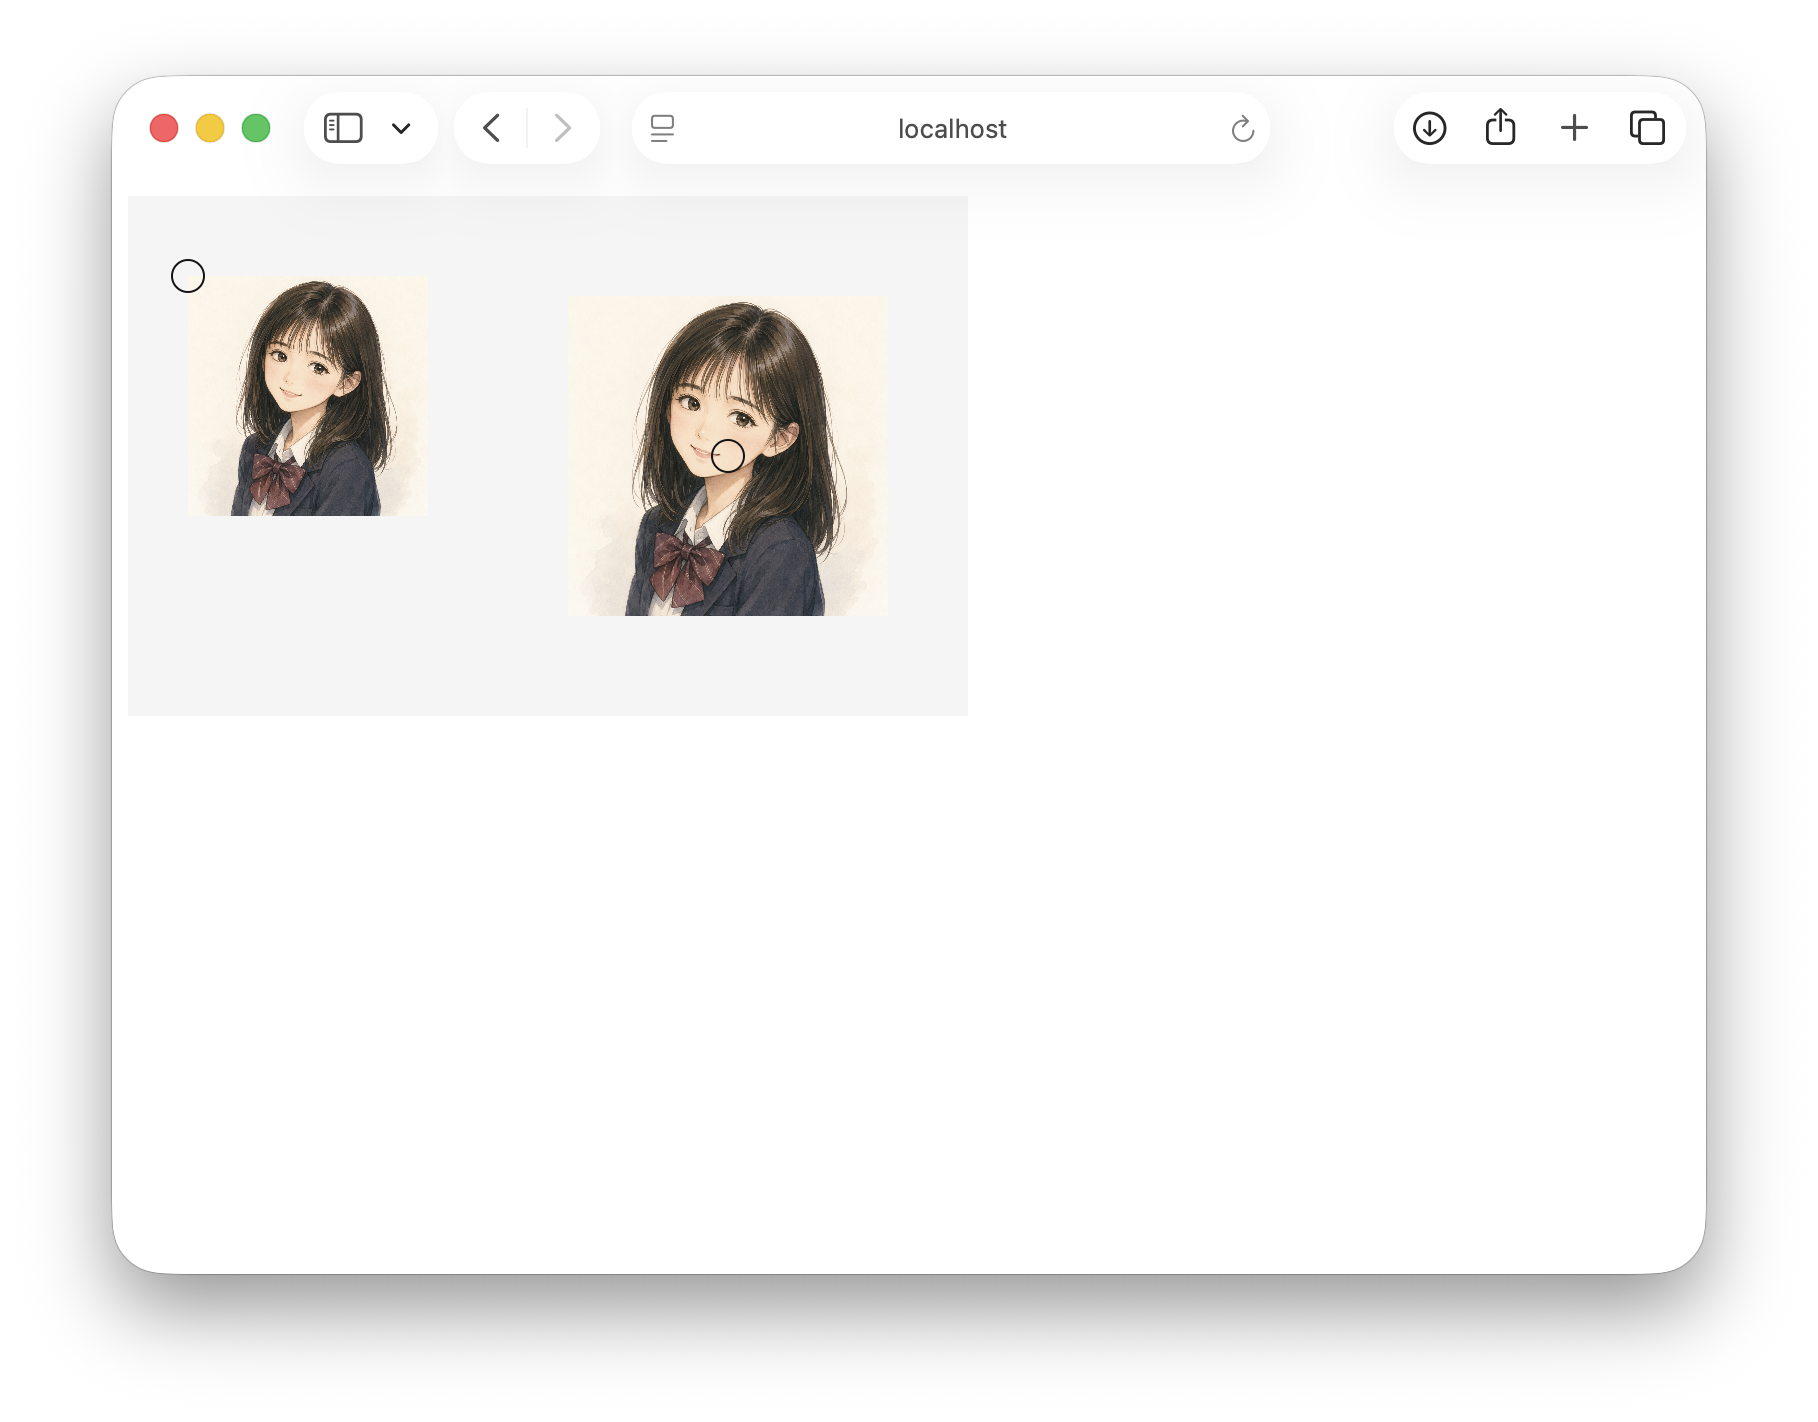
\includegraphics[
        width=0.70\linewidth,
        trim=50 331 419 35,
        clip
    ]{figures/chapter12/image-mode.png}
    \caption{\texttt{CORNER}と\texttt{CENTER}で座標の基準が変わる様子}
    \label{fig:chapter12-image-mode-result}
\end{figure}

図\ref{fig:chapter12-image-mode-result}の左側では、丸印の座標が画像の左上に一致しています。右側では、丸印の座標が画像の中心に一致しています。同じ座標を指定しても、\texttt{imageMode}によって画像が置かれる範囲が変わります。

\section{マウスで画像を動かす}

画像も、図形と同じように座標を変えることで動かせます。次のサンプルでは、画像をマウスの位置に表示し、マウスボタンを押している間だけ大きく表示します。

\begin{listing}[htbp]
\inputminted{ts}{listings/chapter12/image-follow-mouse.ts}
\caption{マウスの位置に画像を表示する}
\label{lst:chapter12-image-follow-mouse}
\end{listing}

\texttt{p.mouseIsPressed}は、マウスボタンが押されているかどうかを表す\texttt{boolean}型の値です。第6章で学んだ条件分岐を使えば、画像の大きさや表示位置を操作できます。

\begin{figure}[htbp]
    \centering
    \begin{minipage}[t]{0.47\linewidth}
        \centering
        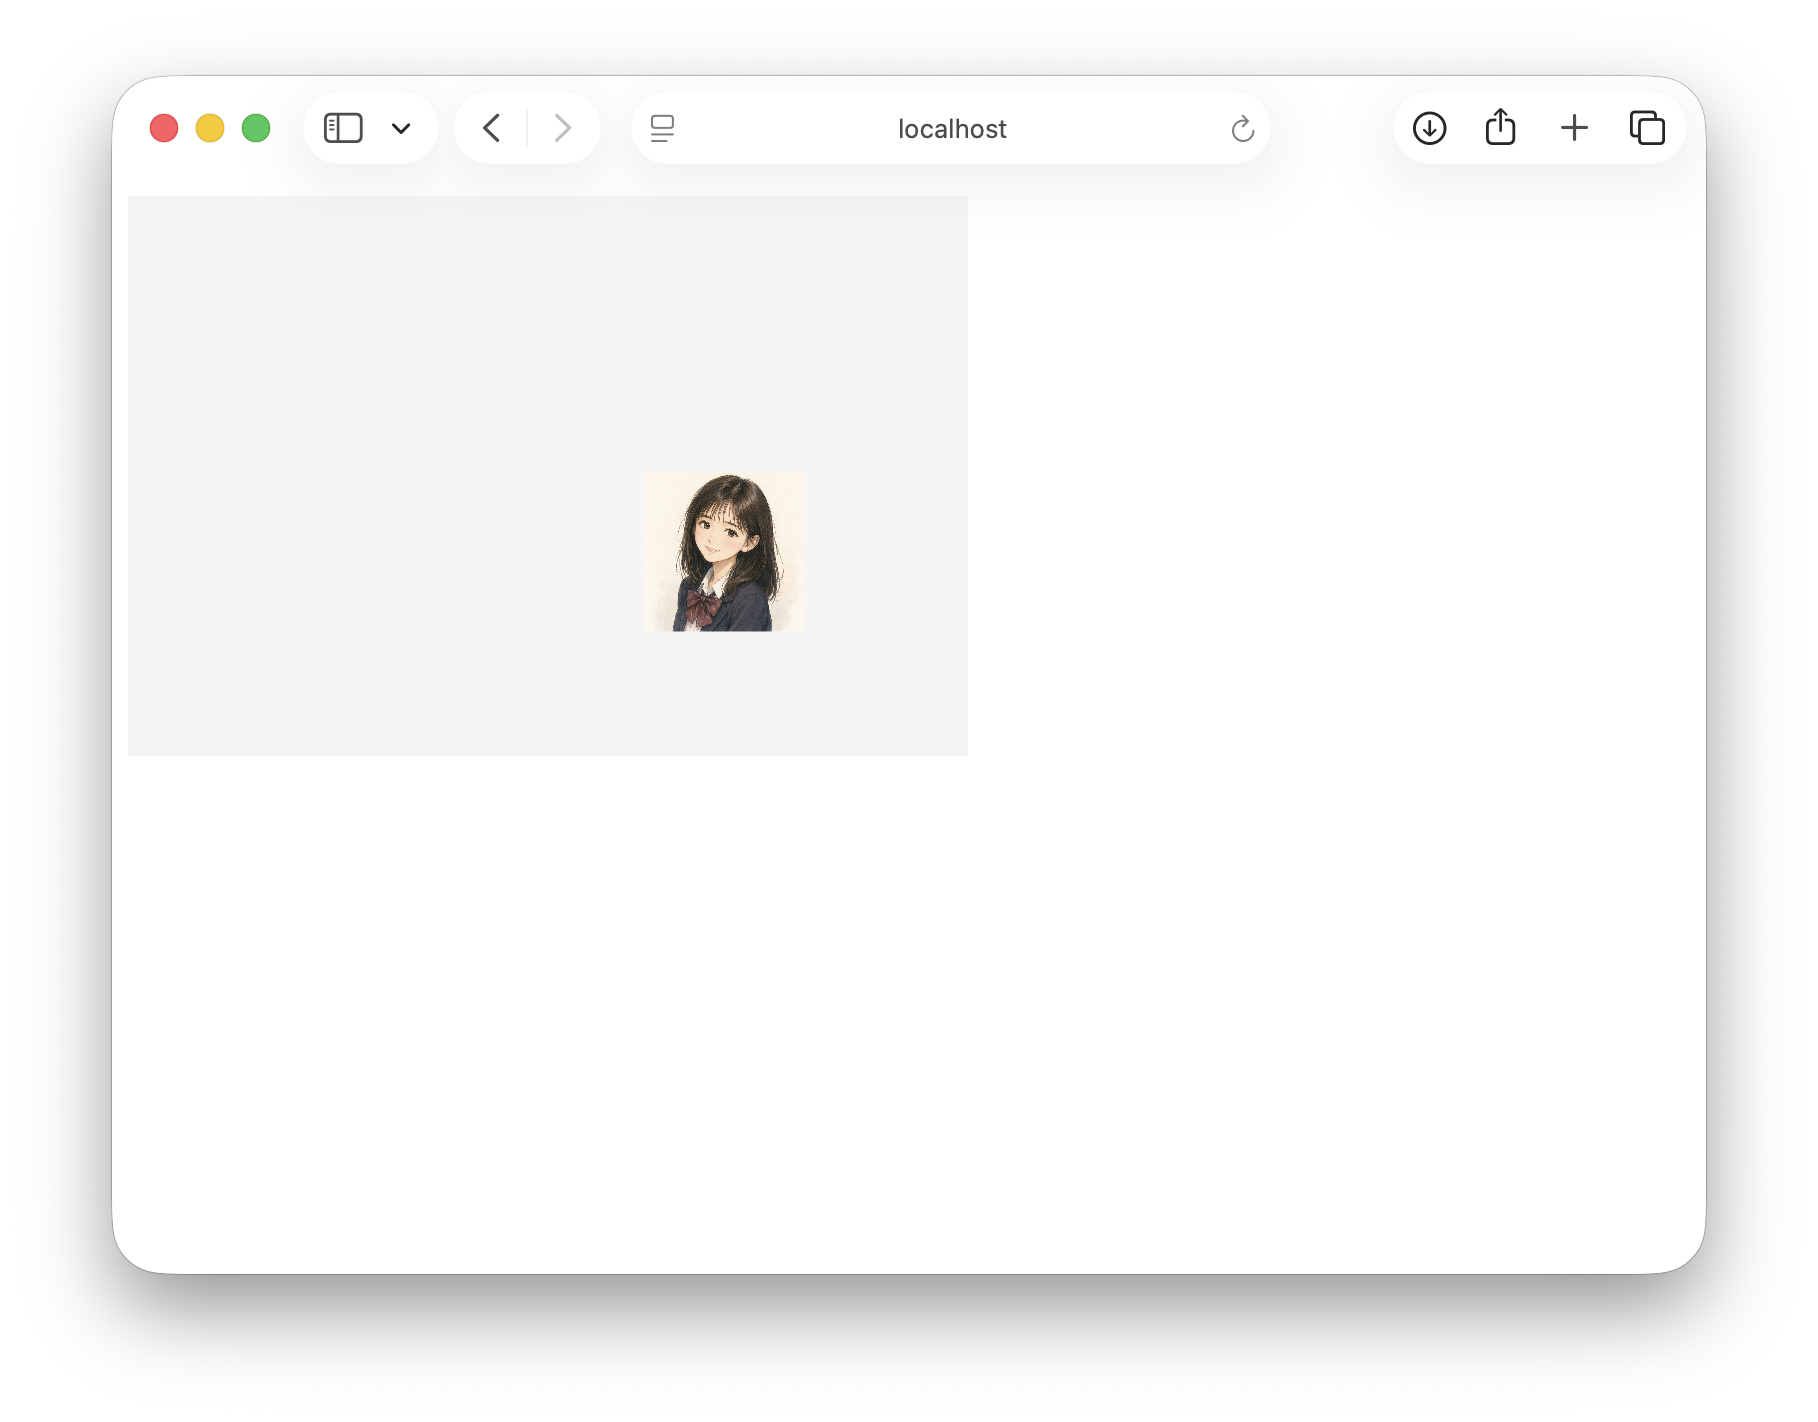
\includegraphics[
            width=\linewidth,
            trim=50 316 419 35,
            clip
        ]{figures/chapter12/follow-mouse-01.png}

        \small マウスを中央付近へ動かした場合
    \end{minipage}
    \hfill
    \begin{minipage}[t]{0.47\linewidth}
        \centering
        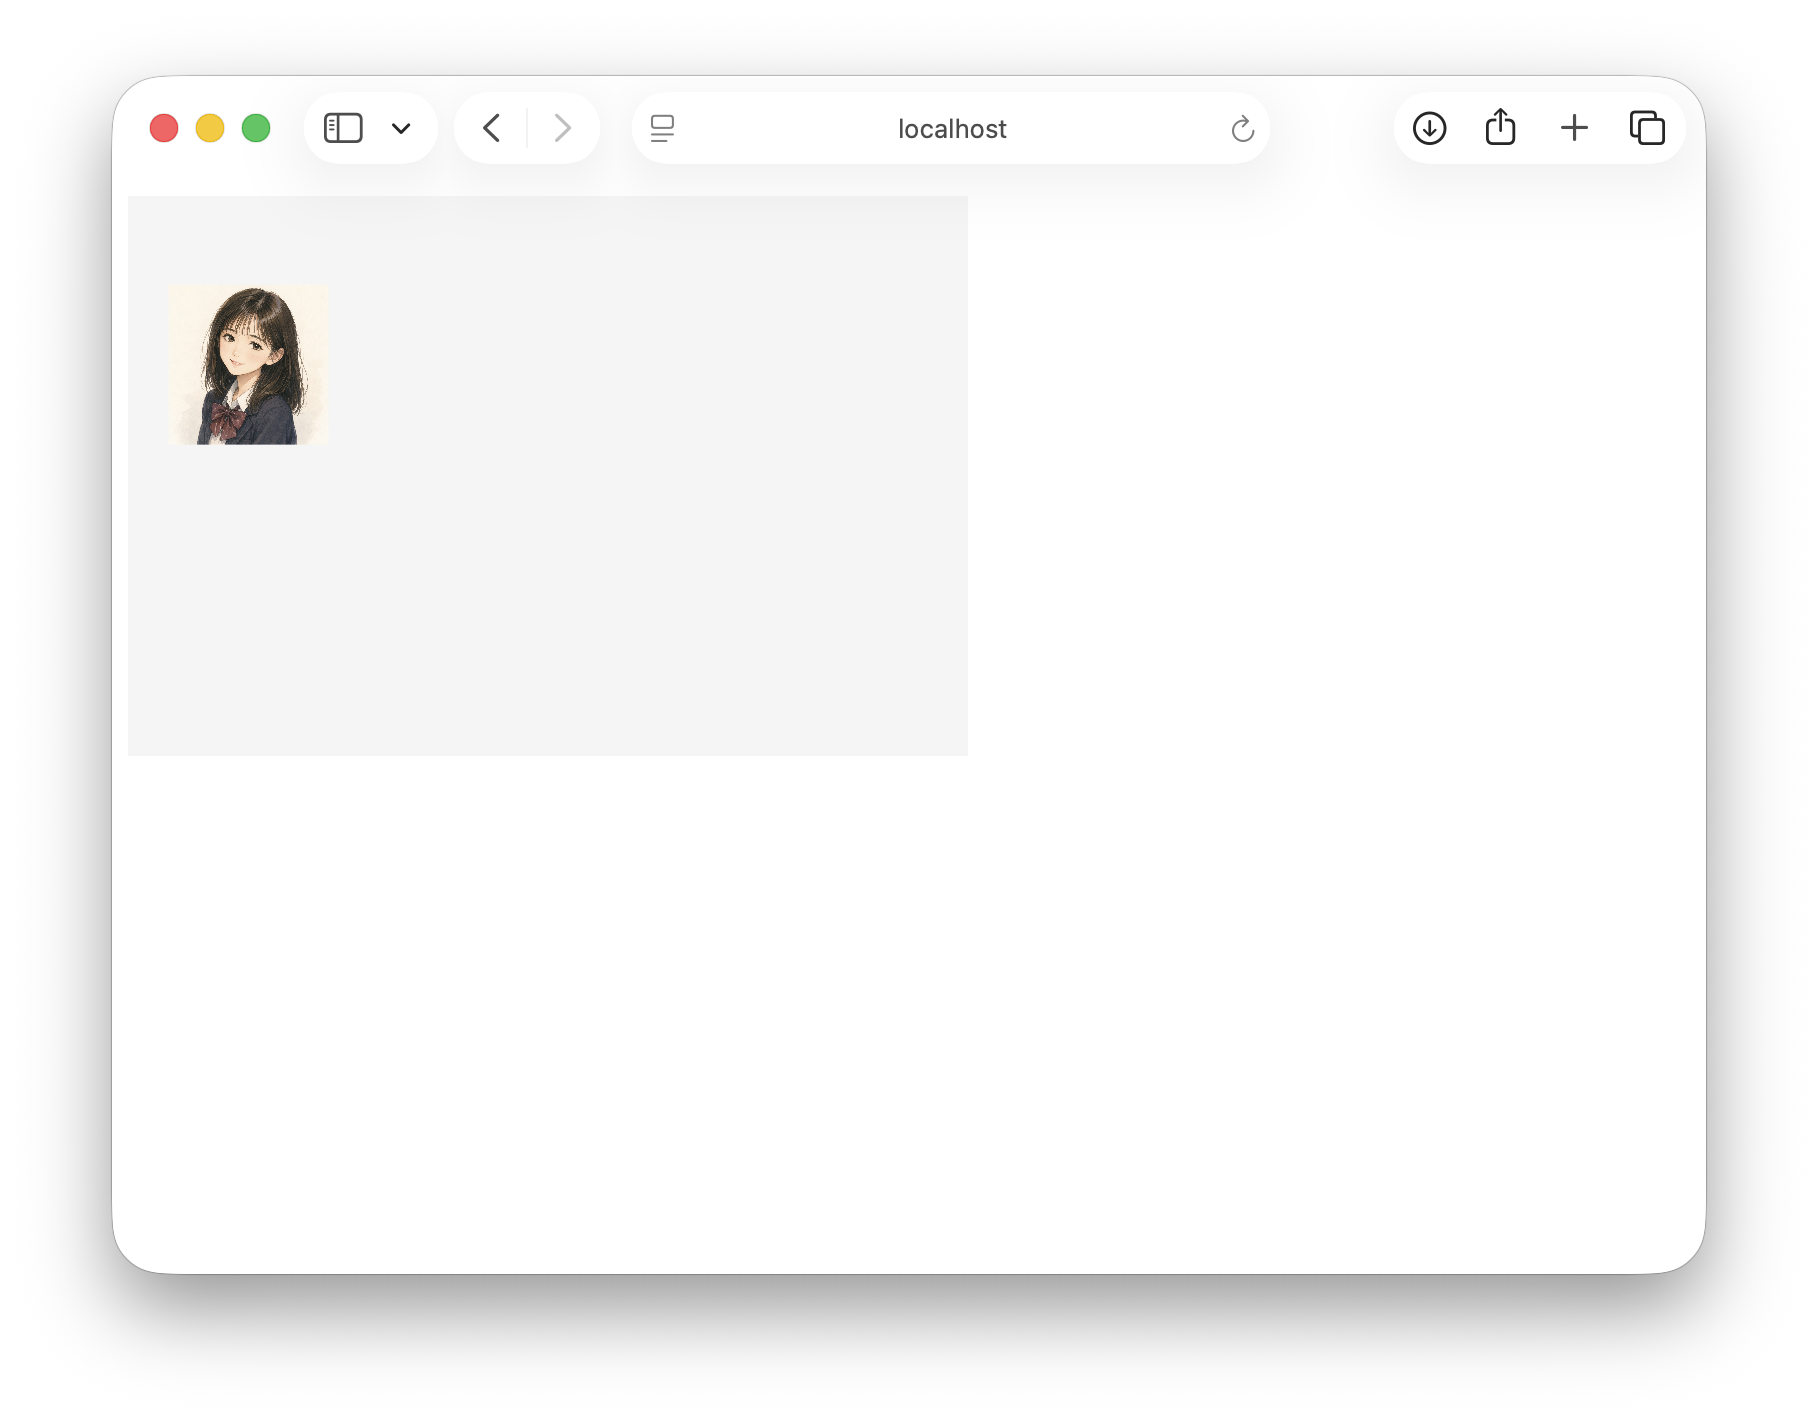
\includegraphics[
            width=\linewidth,
            trim=50 316 419 35,
            clip
        ]{figures/chapter12/follow-mouse-02.png}

        \small マウスを左上付近へ動かした場合
    \end{minipage}
    \caption{マウスの移動に画像が追随する様子}
    \label{fig:chapter12-follow-mouse-results}
\end{figure}

図\ref{fig:chapter12-follow-mouse-results}では、マウスを動かした前後の画面を並べています。\texttt{p.mouseX}と\texttt{p.mouseY}を画像の座標に使うことで、画像の中心がマウスの位置へ追随します。

\begin{pointbox}{画像も座標で動かせる}
画像は特別なものに見えますが、表示するときには座標と大きさを指定します。そのため、円や四角形と同じように、変数、条件分岐、繰り返し処理と組み合わせられます。
\end{pointbox}

\section{画像と文字を組み合わせる}

画像だけでなく、画像の上や下に文字を重ねると、カード、タイトル画面、ゲームの説明表示のようなものを作れます。描画順序はこれまでと同じで、後に描いたものほど手前に表示されます。

\begin{listing}[htbp]
\inputminted{ts}{listings/chapter12/image-caption-card.ts}
\caption{画像に説明文を重ねる}
\label{lst:chapter12-image-caption-card}
\end{listing}

このサンプルでは、最初に画像を描き、その後に半透明の長方形と文字を描いています。画像の上に読みやすい文字を置きたいときは、文字の背後に白や黒の半透明の長方形を置くと見やすくなります。

\begin{figure}[htbp]
    \centering
    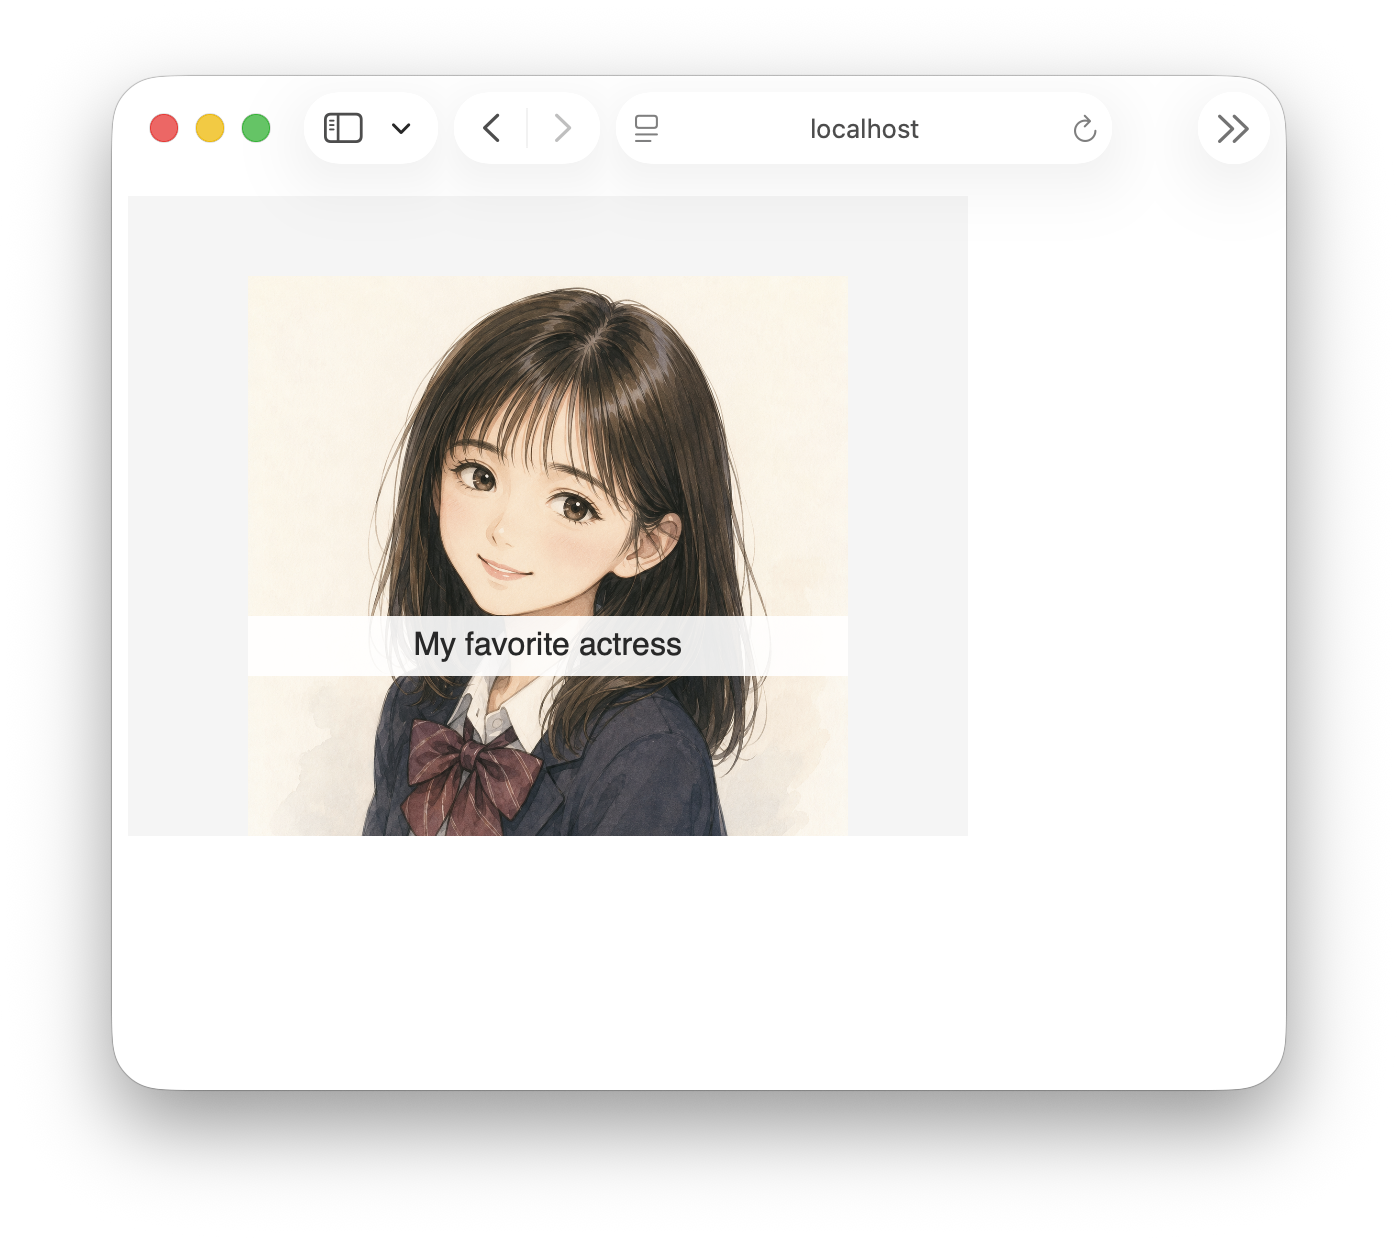
\includegraphics[
        width=0.62\linewidth,
        trim=50 179 204 35,
        clip
    ]{figures/chapter12/image-and-caption.png}
    \caption{画像の上へ半透明の長方形と文字を重ねた実行画面}
    \label{fig:chapter12-image-caption-result}
\end{figure}

図\ref{fig:chapter12-image-caption-result}では、画像を描いた後に半透明の白い長方形を描き、その上へ文字を描いています。文字の背後を少し明るくすることで、画像の色に左右されず説明文を読みやすくできます。

\begin{notebox}{描画順序を意識する}
文字を先に描いてから画像を描くと、画像が文字を隠してしまいます。背景、画像、文字のように、奥に置きたいものから順番に描きましょう。
\end{notebox}

\begin{notebox}{フォントを扱う順番}
まずはブラウザの標準フォントで文字を表示します。\texttt{p.textSize}は文字の大きさを、\texttt{p.textAlign}は文字の揃え方を設定します。特別な書体が必要になった段階で、Webフォントや\texttt{p.loadFont}を学びます。
\end{notebox}

\section{よくある間違い}

文字と画像では、ファイル名、描画順序、読み込みのタイミングでつまずきやすくなります。
エラーが出たときは、まず「ファイルの場所」「ファイル名」「\texttt{loadImage}で読み込んでいるか」
を確認しましょう。

\begin{mistakebox}{画像ファイルの場所や名前を間違える}
\texttt{p.loadImage("images/sample.png")}と書いた場合、実際にその場所に\texttt{sample.png}が必要です。大文字と小文字、拡張子、フォルダ名も一致させましょう。
\end{mistakebox}

\begin{mistakebox}{文字が画像に隠れる}
後から描いたものほど手前に表示されます。画像の上に文字を表示したい場合は、画像を描いた後に文字を描きます。
\end{mistakebox}

\begin{mistakebox}{\texttt{textAlign}の設定が残る}
\texttt{textAlign}の設定は、その後に描く文字にも影響します。別の場所で左揃えに戻したい場合は、\texttt{p.textAlign(p.LEFT, p.BASELINE)}のように設定し直します。
\end{mistakebox}

\section{まとめ}

この章では、文字列と画像を画面に表示する方法を学びました。文字列は\texttt{string}型で扱い、\texttt{text}、\texttt{textSize}、\texttt{textAlign}、\texttt{textWidth}を使って表示します。

画像は\texttt{p5.Image}型で扱い、\texttt{loadImage}関数を使って読み込みます。
ただし、\texttt{p.setup = async (): Promise<void> => \{ ... \};}のように、\texttt{async}を付けて書き、\texttt{loadImage}の前に\texttt{await}を付ける必要があります。

表示には\texttt{p.image}を使い、\texttt{imageMode}や表示サイズを指定することで、図形と同じように位置や大きさを制御できます。

\section{演習問題}

この章の演習では、文字と画像の表示を少しずつ変更しながら、作品の画面を作る練習をします。最初は文字列や座標を変えるだけでよいので、表示結果を確認しながら進めましょう。

\begin{enumerate}
    \item \texttt{basic-text.ts}の\texttt{message}を自分の好きな文字列に変更してください。
    \item \texttt{basic-text.ts}で、文字の色と大きさを変更してください。
    \item \texttt{text-align-box.ts}で、文字を左揃え、右揃えに変更して違いを確認してください。
    \item \texttt{moving-text.ts}で、文字列の移動速度を変えてください。
    \item \texttt{moving-text.ts}で、文字列が右から左ではなく、左から右へ動くようにしてください。
    \item \texttt{load-image-basic.ts}で、読み込む画像ファイル名を変更してください。
    \item \texttt{image-size-and-mode.ts}で、\texttt{p.CORNER}と\texttt{p.CENTER}の違いを説明してください。
    \item \texttt{image-follow-mouse.ts}で、マウスを押しているときに画像が小さく、離しているときに大きくなるようにしてください。
    \item \texttt{image-caption-card.ts}で、画像の下に表示する説明文を2行に増やしてください。
    \item 挑戦問題として、画像、タイトル、説明文、ボタン風の図形を組み合わせて、ゲームのタイトル画面を作ってください。
\end{enumerate}

\chapter{多次元配列}
\label{chap:multidimensional-arrays}

この章では、2次元配列を使って、表や盤面のようなデータを扱う方法を学びます。第10章では、配列を使って複数の円や棒の長さをまとめて扱いました。そこでは、\texttt{circleX[0]}、\texttt{circleX[1]}のように、1つの添え字番号で要素を選びました。

格子状に並んだマス、ゲームの盤面、画像のピクセルに近い情報を扱うときは、「何番目の行か」と「何番目の列か」の2つで場所を指定できると便利です。このようなデータを扱うために、2次元配列を使います。

\section{この章の概要}

この章では、色の格子、クリックされた場所の記録、オセロ風の盤面を題材に、2次元配列の使い方を学びます。

この章で扱う主な内容は次の通りです。

\begin{itemize}
    \item 2次元配列の考え方
    \item 行と列を使った要素の指定
    \item 2次元配列の型と\texttt{length}を使った行・列数
    \item 二重の\texttt{for}文
    \item マウス座標から行と列を求める方法
    \item 盤面を2次元配列で表す方法
\end{itemize}

\section{2次元配列とは何か}

2次元配列は、配列の中に配列が入っている形のデータです。1次元配列が横一列の箱だとすると、2次元配列は行と列を持つ表のようなものとして考えられます。

\begin{figure}[htbp]
    \centering
    \begin{tikzpicture}[
        cell/.style={rectangle, draw, minimum width=18mm, minimum height=10mm, align=center},
        index/.style={align=center}
    ]
        \foreach \row in {0,1,2} {
            \foreach \column in {0,1,2,3} {
                \node[cell] at (\column*1.8, -\row*1.0)
                    {\texttt{[\row][\column]}};
            }
        }
        \foreach \row in {0,1,2} {
            \node[index] at (-1.2, -\row*1.0) {行\\\texttt{\row}};
        }
        \foreach \column in {0,1,2,3} {
            \node[index] at (\column*1.8, 0.8) {列\\\texttt{\column}};
        }
    \end{tikzpicture}
    \caption{2次元配列を行と列で考える}
    \label{fig:chapter13-row-column}
\end{figure}

TypeScriptでは、数値の2次元配列を\texttt{number[][]}と書きます。これは「\texttt{number[]}の配列」、つまり「数値の配列が並んだもの」と読むこともできます。

\begin{pointbox}{添え字は2つになる}
2次元配列では、\texttt{numbers[row][column]}のように添え字を2つ使います。この章では、1つ目を行、2つ目を列として読むことにします。
\end{pointbox}

\section{表のように数値を表示する}

まずは、数値を2次元配列に保存し、表のように表示するプログラムを見てみます。行と列を使って、どのマスにどの値を表示するかを決めます。

\begin{listing}[htbp]
\inputminted{ts}{listings/chapter13/grid-numbers.ts}
\caption{2次元配列の数値を表のように表示する}
\label{lst:chapter13-grid-numbers}
\end{listing}

\texttt{numbers[0][0]}は左上の値、\texttt{numbers[0][1]}は同じ行の次の値を表します。\texttt{numbers[1][0]}は、1行下がった最初の値です。

\begin{center}
\begin{tabular}{lll}
\toprule
式 & 表す場所 & 値 \\
\midrule
\texttt{numbers[0][0]} & 0行0列 & \texttt{1} \\
\texttt{numbers[0][3]} & 0行3列 & \texttt{4} \\
\texttt{numbers[2][0]} & 2行0列 & \texttt{9} \\
\texttt{numbers[2][3]} & 2行3列 & \texttt{12} \\
\bottomrule
\end{tabular}
\end{center}

\begin{notebox}{行と列の順番を決めて読む}
本書では、2次元配列の添え字を\texttt{[row][column]}の順に統一します。
\end{notebox}

\section{二重のfor文}

2次元配列のすべての要素を調べるには、\texttt{for}文を2つ重ねます。外側の\texttt{for}文で行を選び、内側の\texttt{for}文でその行の列を順番に選びます。

\begin{figure}[htbp]
    \centering
    \begin{tikzpicture}[
        cell/.style={rectangle, draw, minimum width=16mm, minimum height=9mm, align=center},
        arrow/.style={->, thick}
    ]
        \foreach \row in {0,1,2} {
            \foreach \column in {0,1,2,3} {
                \node[cell] (c\row\column) at (\column*1.6, -\row*0.9)
                    {\texttt{\row,\column}};
            }
        }
        \draw[arrow, red] (c00.north) to[bend left=20] (c01.north);
        \draw[arrow, red] (c01.north) to[bend left=20] (c02.north);
        \draw[arrow, red] (c02.north) to[bend left=20] (c03.north);
        \draw[arrow, blue] (c03.east) to[bend left=20] (c10.east);
        \draw[arrow, red] (c10.north) to[bend left=20] (c11.north);
        \draw[arrow, red] (c11.north) to[bend left=20] (c12.north);
        \draw[arrow, red] (c12.north) to[bend left=20] (c13.north);
        \node[align=left] at (3.2, -3.3)
            {赤: 列を進める\\青: 次の行へ進む};
    \end{tikzpicture}
    \caption{二重の\texttt{for}文で行と列を順に見る}
    \label{fig:chapter13-nested-loop}
\end{figure}

サンプル\ref{lst:chapter13-grid-numbers}では、\texttt{row}と\texttt{column}を使って、描画位置も計算しています。列が増えると右へ進み、行が増えると下へ進みます。

\begin{pointbox}{外側が行、内側が列}
表や盤面を左上から順に処理するときは、外側の\texttt{for}文で行、内側の\texttt{for}文で列を動かすと読みやすくなります。
\end{pointbox}

\section{\texttt{length}で行数と列数を調べる}

2次元配列では、\texttt{values.length}で行数を調べられます。ある行の列数は、\texttt{values[row].length}で調べます。これは、2次元配列が「配列の中に配列が入っている形」だからです。

\begin{listing}[htbp]
\inputminted{ts}{listings/chapter13/sum-grid.ts}
\caption{\texttt{length}を使って2次元配列の合計を求める}
\label{lst:chapter13-sum-grid}
\end{listing}

\texttt{sumGrid}関数は、\texttt{number[][]}型の引数を受け取り、すべての要素を足して返します。第8章で学んだ関数、第10章で学んだ配列、第7章で学んだ繰り返しを組み合わせた例です。

\section{色の格子を作る}

p5.jsでは色を\texttt{p5.Color}型で扱います。\texttt{p5.Color[][]}は色の2次元配列で、格子の各マスの色を保存できます。

\begin{listing}[htbp]
\inputminted{ts}{listings/chapter13/random-color-grid.ts}
\caption{\texttt{p5.Color[][]}で色の格子を作る}
\label{lst:chapter13-random-color-grid}
\end{listing}

このサンプルでは、\texttt{cellColors[row][column]}に各マスの色を保存しています。まず\texttt{cellColors[row] = [];}で1行分の配列を用意し、その後で各列の色を入れています。

\begin{notebox}{行を先に用意する}
\texttt{cellColors[row][column]}に値を入れる前に、\texttt{cellColors[row] = [];}でその行を作っておく必要があります。行を作らないまま列の値を入れようとすると、実行時にエラーになります。
\end{notebox}

\section{クリックしたマスを覚える}

2次元配列は、マスごとの状態を覚える用途にも向いています。たとえば、「そのマスが塗られているかどうか」は\texttt{boolean}型で表せます。これを格子全体に広げると\texttt{boolean[][]}になります。

\begin{listing}[htbp]
\inputminted{ts}{listings/chapter13/click-toggle-grid.ts}
\caption{\texttt{boolean[][]}でクリックしたマスを切り替える}
\label{lst:chapter13-click-toggle-grid}
\end{listing}

マウスの座標はピクセル単位です。一方、配列の添え字は0、1、2のような整数です。そのため、\texttt{Math.floor(p.mouseX / cellSize)}のようにして、マウスのx座標から列番号を求めます。

\begin{figure}[htbp]
    \centering
    \begin{tikzpicture}[
        font=\small,
        calculation/.style={draw, rounded corners=2pt, fill=blue!5, minimum width=42mm, minimum height=9mm, align=center},
        result/.style={draw, rounded corners=2pt, fill=green!8, minimum width=35mm, minimum height=9mm, align=center}
    ]
        \foreach \row in {0,1,2,3} {
            \foreach \column in {0,1,2,3,4} {
                \draw[gray] (\column*1.05,-\row*1.05)
                    rectangle +(1.05,-1.05);
            }
        }
        \fill[orange!25] (2.10,-1.05) rectangle +(1.05,-1.05);
        \draw[orange!80!black, very thick]
            (2.10,-1.05) rectangle +(1.05,-1.05);
        \fill[red!75!black] (2.36,-1.66) circle (2.2pt);

        \foreach \column in {0,1,2,3,4} {
            \node[font=\scriptsize] at (\column*1.05+0.525,0.28)
                {列\column};
        }
        \foreach \row in {0,1,2,3} {
            \node[font=\scriptsize, anchor=east]
                at (-0.12,-\row*1.05-0.525) {行\row};
        }
        \node[align=center, anchor=north] at (2.62,-4.45)
            {クリック位置\\\texttt{(135, 95)}};
        \draw[->, red!75!black, thick]
            (2.62,-4.32) -- (2.38,-1.82);

        \node[calculation] (mouse) at (9.6,0)
            {\texttt{p.mouseX = 135}、\texttt{p.mouseY = 95}};
        \node[calculation] (columnCalc) at (7.45,-1.55)
            {\texttt{135 / 60 = 2.25}\\x座標をマス幅で割る};
        \node[calculation] (rowCalc) at (11.75,-1.55)
            {\texttt{95 / 60 = 1.58...}\\y座標をマス高さで割る};
        \node[result] (columnResult) at (7.45,-3.05)
            {\texttt{Math.floor(...)}\\\texttt{column = 2}};
        \node[result] (rowResult) at (11.75,-3.05)
            {\texttt{Math.floor(...)}\\\texttt{row = 1}};
        \node[result, minimum width=56mm] (array) at (9.6,-4.55)
            {\texttt{isPainted[row][column]}\\
             \texttt{isPainted[1][2]}};

        \draw[->, thick] (mouse.south west) -- (columnCalc.north);
        \draw[->, thick] (mouse.south east) -- (rowCalc.north);
        \draw[->, thick] (columnCalc) -- (columnResult);
        \draw[->, thick] (rowCalc) -- (rowResult);
        \draw[->, thick] (columnResult.south) -- (array.north west);
        \draw[->, thick] (rowResult.south) -- (array.north east);
    \end{tikzpicture}
    \caption{マウス座標からクリックされた行と列を求める流れ}
    \label{fig:chapter13-mouse-to-row-column}
\end{figure}

図\ref{fig:chapter13-mouse-to-row-column}では、マスの大きさを60ピクセルとしています。x座標から列番号を、y座標から行番号を別々に求め、最後に\texttt{isPainted[row][column]}の順で配列の要素を選びます。

\begin{center}
\begin{tabular}{lll}
\toprule
計算 & 意味 & 例 \\
\midrule
\texttt{p.mouseX / cellSize} & x座標をマスの大きさで割る & \texttt{135 / 60 = 2.25} \\
\texttt{Math.floor(...)} & 小数点以下を切り捨てる & \texttt{2.25}から\texttt{2} \\
\texttt{isPainted[row][column]} & クリックされたマスの状態 & \texttt{true}または\texttt{false} \\
\bottomrule
\end{tabular}
\end{center}

\begin{notebox}{整数の添え字を作る}
TypeScriptの\texttt{number}型では、整数と小数を分けません。配列の添え字として使う値は、\texttt{Math.floor}で小数点以下を切り捨てて整数にしてから使います。
\end{notebox}

\begin{mistakebox}{範囲外の添え字に注意する}
マウスがキャンバスの外や端にあると、存在しない行や列を指定してしまうことがあります。サンプルでは、\texttt{0 <= row}や\texttt{row < isPainted.length}を使って、範囲内かどうかを確認してから配列を書き換えています。
\end{mistakebox}

\section{盤面を2次元配列で表す}

2次元配列は、ボードゲームの盤面を表すときにもよく使われます。ここでは、オセロのルールをすべて作るのではなく、「4行4列の小さな盤面に黒と白の石を置く」という部分だけを作ります。

\begin{listing}[htbp]
\inputminted[firstline=1,lastline=45]{ts}{listings/chapter13/simple-board.ts}
\caption{\texttt{number[][]}で簡単な盤面を表す前半}
\label{lst:chapter13-simple-board-draw}
\end{listing}

\begin{listing}[htbp]
\inputminted[firstline=47,lastline=67]{ts}{listings/chapter13/simple-board.ts}
\caption{\texttt{number[][]}で簡単な盤面を表す後半}
\label{lst:chapter13-simple-board-click}
\end{listing}

\texttt{board[row][column]}には、マスの状態を表す数値を保存しています。\texttt{empty}は何も置かれていないマス、\texttt{black}は黒い石、\texttt{white}は白い石です。サンプルは1つのファイルですが、紙面では読みやすいように前半と後半に分けて掲載しています。

\begin{figure}[htbp]
    \centering
    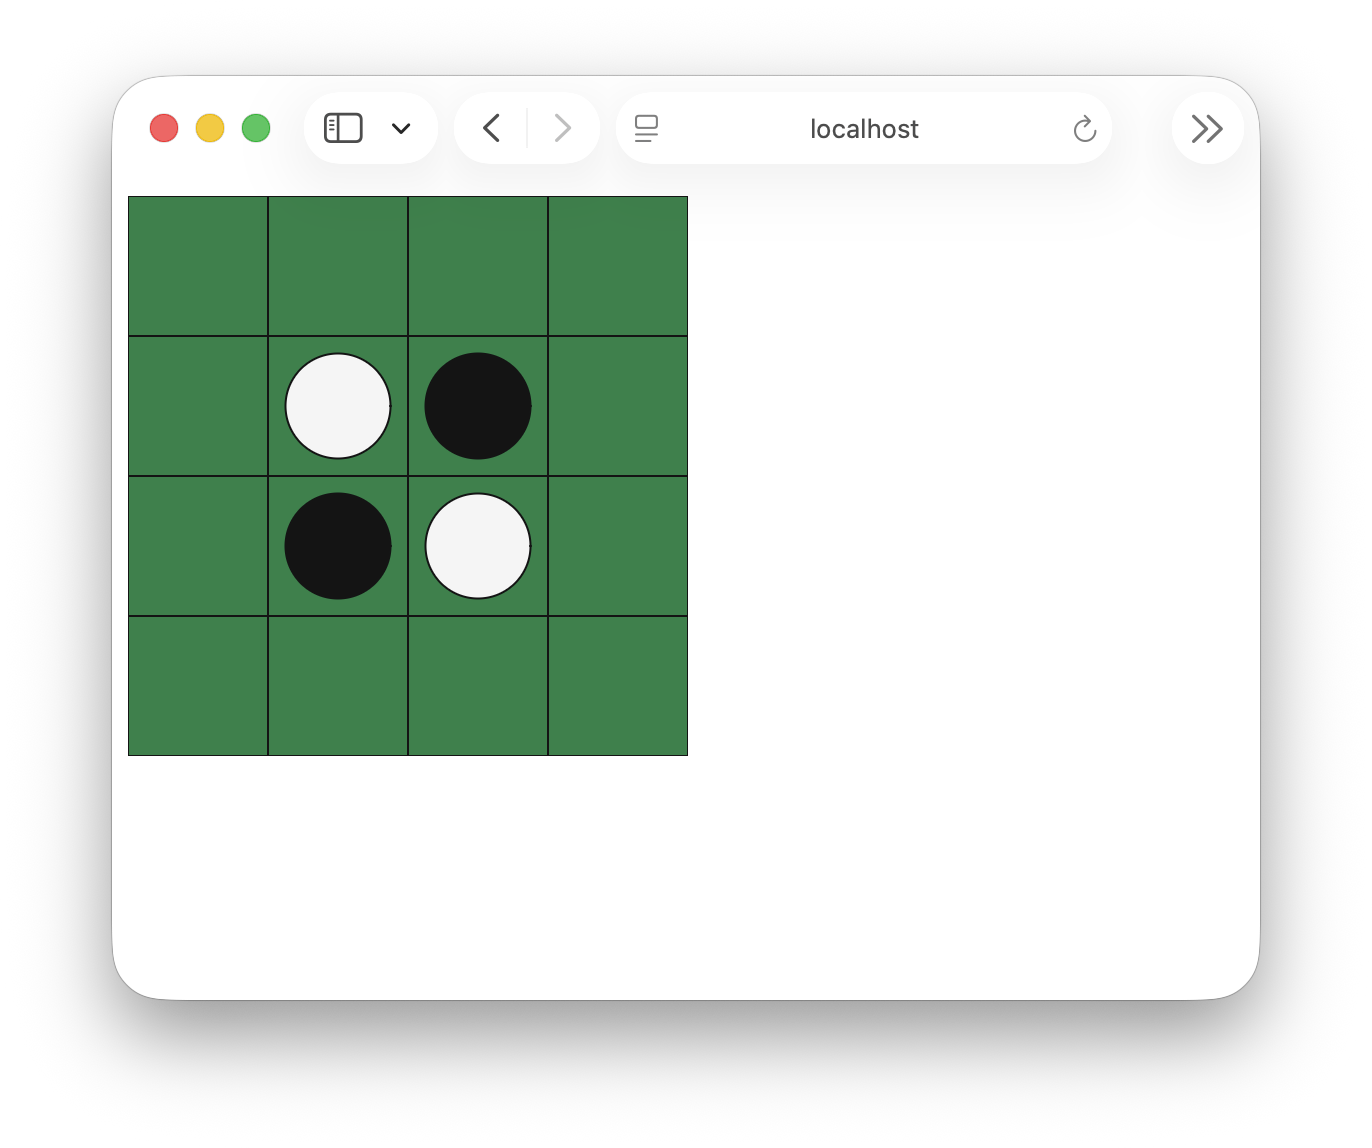
\includegraphics[
        width=0.50\linewidth,
        trim=50 174 326 35,
        clip
    ]{figures/chapter13/board.png}
    \caption{2次元配列の値から描いた4行4列の盤面}
    \label{fig:chapter13-simple-board-result}
\end{figure}

図\ref{fig:chapter13-simple-board-result}では、2次元配列の各要素が1つのマスに対応しています。\texttt{empty}のマスには石を描かず、\texttt{black}と\texttt{white}のマスにはそれぞれ黒と白の円を描いています。

\begin{pointbox}{数値に意味の名前を付ける}
\texttt{0}、\texttt{1}、\texttt{2}を直接コードの中に書くと、あとで読んだときに意味が分かりにくくなります。\texttt{empty}、\texttt{black}、\texttt{white}のような名前を付けると、盤面の状態を読みやすくできます。
\end{pointbox}

\section{よくある間違い}

2次元配列では、添え字が2つあるため、1次元配列よりも間違える場所が増えます。特に、行と列の順番、行の初期化、範囲外アクセスに注意しましょう。

\begin{mistakebox}{行と列を逆にしてしまう}
\texttt{board[row][column]}で統一しているのに、途中で\texttt{board[column][row]}と書くと、思った場所と違うマスを操作してしまいます。変数名を\texttt{row}、\texttt{column}にしておくと読み間違いを減らせます。
\end{mistakebox}

\begin{mistakebox}{行の配列を作り忘れる}
\texttt{cellColors[row][column]}に値を入れる前に、\texttt{cellColors[row] = [];}が必要です。2次元配列は、外側の配列と内側の配列を順に用意する、と考えましょう。
\end{mistakebox}

\begin{mistakebox}{すべての行の列数が同じだと思い込む}
TypeScriptの2次元配列は、行ごとに列数が違っていても作れてしまいます。そのため、列数を調べるときは\texttt{values[0].length}だけでなく、繰り返し中の\texttt{values[row].length}を使うと安全です。
\end{mistakebox}

\begin{mistakebox}{マウス座標をそのまま添え字に使う}
\texttt{p.mouseX}や\texttt{p.mouseY}はピクセル単位の数値です。そのまま\texttt{board[p.mouseY][p.mouseX]}のように使うと、ほとんどの場合は範囲外になります。マスの大きさで割って、整数に変換してから使います。
\end{mistakebox}

\section{まとめ}

この章では、2次元配列を使って、表、色の格子、クリックできるマス、簡単な盤面を表す方法を学びました。2次元配列では、\texttt{values[row][column]}のように、行と列の2つの添え字で要素を指定します。

2次元配列を扱うときは、二重の\texttt{for}文、\texttt{length}、行と列の命名が重要になります。ゲームの盤面やマップを作るときにも使う考え方なので、最初は小さな表から練習して、少しずつマスの状態を増やしていきましょう。

\section{演習問題}

この章の演習では、2次元配列の値、行数、列数、クリック処理を少しずつ変更します。いきなり大きな盤面を作るのではなく、小さな格子で動作を確認しながら進めましょう。

\begin{enumerate}
    \item \texttt{grid-numbers.ts}で、\texttt{numbers}の値を自分で変更してください。
    \item \texttt{grid-numbers.ts}で、4行3列の表になるように配列を書き換えてください。
    \item \texttt{sum-grid.ts}で、合計だけでなく平均も表示してください。
    \item \texttt{random-color-grid.ts}で、行数と列数を変更してください。
    \item \texttt{random-color-grid.ts}で、四角形ではなく円を格子状に描いてください。
    \item \texttt{click-toggle-grid.ts}で、クリックしたマスの色を別の色に変更してください。
    \item \texttt{click-toggle-grid.ts}で、マスの大きさを変えても動くように確認してください。
    \item \texttt{simple-board.ts}で、最初に置かれている石の位置を変更してください。
    \item \texttt{simple-board.ts}で、黒の番か白の番かを文字で表示してください。
    \item 挑戦問題として、2次元配列を使って、クリックで壁を置ける迷路の編集画面を作ってください。
\end{enumerate}

\chapter{継承}
\label{chap:inheritance}

この章では、クラスをもとにして別のクラスを作る「継承」について学びます。第11章では、\texttt{Ball}クラスや\texttt{FallingSquare}クラスを作り、フィールド、コンストラクタ、メソッド、インスタンスの考え方を学びました。

円を落とすクラスと正方形を落とすクラスを見比べると、位置、速さ、画面外に出たときの処理など、よく似た部分がたくさんあります。継承は、このような「似ているクラス」を整理し、共通する部分を1か所にまとめるための仕組みです。

\section{この章の概要}

この章では、点を少しずつ揺らすクラスをもとに、正方形を表示するクラスへ拡張する例を通して、継承の考え方を学びます。

この章で扱う主な内容は次の通りです。

\begin{itemize}
    \item 似たクラスに共通する部分を見つける
    \item 親クラスと子クラス
    \item \texttt{extends}による継承
    \item \texttt{super}による親クラスのコンストラクタ呼び出し
    \item 子クラスでメソッドを上書きする方法
    \item 親クラス型の配列で子クラスをまとめる
    \item 第11章の落ちる図形への応用
\end{itemize}

\section{第11章からのつながり}

第11章では、円を表す\texttt{Ball}クラスを作り、その後で正方形を表す\texttt{FallingSquare}クラスも作りました。円と正方形は見た目こそ違いますが、どちらも「位置を持つ」「下に動く」「画面の下に出たら上に戻る」という点ではよく似ています。

\begin{center}
\begin{tabular}{lll}
\toprule
処理や情報 & 円のクラス & 正方形のクラス \\
\midrule
中心のx座標 & 必要 & 必要 \\
中心のy座標 & 必要 & 必要 \\
下向きの速さ & 必要 & 必要 \\
色 & 必要 & 必要 \\
画面外に出たら戻る処理 & 必要 & 必要 \\
描画方法 & 円を描く & 正方形を描く \\
\bottomrule
\end{tabular}
\end{center}

この表を見ると、違いは主に「どの図形を描くか」です。つまり、動き方は共通で、描き方だけが違うと考えられます。このようなときに継承を使うと、共通する動き方を親クラスにまとめ、描き方だけを子クラスで変えられます。

\begin{notebox}{継承は重複を減らすための道具}
継承は「コードを短くする魔法」ではありません。似ているクラスの共通部分を1か所にまとめ、違う部分だけを子クラスに書くための道具です。
\end{notebox}

\section{まずは揺れる点を作る}

まず、少しずつランダムに動く点を作ります。ここでは、最初に\texttt{JitteringDot}クラスを作ります。\texttt{jitter}は「小刻みに揺れる」という意味です。

\begin{listing}[htbp]
\inputminted{ts}{listings/chapter14/jittering-dot.ts}
\caption{少しずつランダムに動く点}
\label{lst:chapter14-jittering-dot}
\end{listing}

\texttt{JitteringDot}は、\texttt{centerX}と\texttt{centerY}を持ちます。\texttt{update}メソッドでは座標を少しだけ変え、\texttt{display}メソッドでは点を描きます。\texttt{p.constrain}は、値を指定した範囲の中におさめる関数です。

\begin{pointbox}{動きと見た目を分けて考える}
\texttt{update}は位置を変える処理、\texttt{display}は画面に描く処理です。この2つを分けておくと、あとで「動きは同じで見た目だけ違うもの」を作りやすくなります。
\end{pointbox}

\section{継承を使わずに正方形へ作り替える}

点ではなく正方形を揺らしたい場合、継承を使わずに別のクラスを作ることもできます。次のサンプルでは、\texttt{JitteringSquare}クラスを最初から作っています。

\begin{listing}[htbp]
\inputminted{ts}{listings/chapter14/jittering-square-without-inheritance.ts}
\caption{継承を使わずに揺れる正方形を作る}
\label{lst:chapter14-jittering-square-without-inheritance}
\end{listing}

このクラスは正方形を描けますが、\texttt{centerX}、\texttt{centerY}、\texttt{update}の中身が\texttt{JitteringDot}とほとんど同じです。もし移動の範囲や速さを変えたくなったら、点のクラスと正方形のクラスの両方を直す必要があります。

\begin{mistakebox}{コピーして少し変えるだけでは増えるほど大変になる}
似たクラスをコピーして作ると、最初は簡単に見えます。しかし、同じ処理が複数の場所に増えるため、あとで修正するときに直し忘れが起きやすくなります。
\end{mistakebox}

\section{\texttt{extends}でクラスを拡張する}

継承を使うと、あるクラスをもとにして新しいクラスを作れます。もとになるクラスを親クラス、そこから作る新しいクラスを子クラスと呼びます。TypeScriptでは、\texttt{class 子クラス extends 親クラス}のように書きます。

\begin{figure}[htbp]
    \centering
    \begin{tikzpicture}[
        box/.style={rectangle, draw, rounded corners, minimum width=45mm, minimum height=12mm, align=center},
        arrow/.style={->, thick}
    ]
        \node[box, fill=blue!5] (parent) at (0, 0)
            {\texttt{JitteringDot}\\座標と\texttt{update}を持つ};
        \node[box, fill=green!5] (child) at (0, -1.8)
            {\texttt{JitteringSquare}\\一辺の長さと描き方を追加};
        \draw[arrow] (child.north) -- (parent.south);
        \node[align=center] at (3.5, -0.9) {\texttt{extends}\\親クラスをもとにする};
    \end{tikzpicture}
    \caption{親クラスと子クラスの関係}
    \label{fig:chapter14-parent-child}
\end{figure}

次のサンプルでは、\texttt{JitteringSquare}が\texttt{JitteringDot}を継承しています。正方形も点と同じように座標を持ち、\texttt{update}メソッドを使えます。

\begin{listing}[htbp]
\inputminted[firstline=1,lastline=25]{ts}{listings/chapter14/jittering-square-inheritance.ts}
\caption{親クラスになる\texttt{JitteringDot}}
\label{lst:chapter14-jittering-square-inheritance-parent}
\end{listing}

\begin{listing}[htbp]
\inputminted[firstline=27,lastline=43]{ts}{listings/chapter14/jittering-square-inheritance.ts}
\caption{\texttt{JitteringDot}を継承する\texttt{JitteringSquare}}
\label{lst:chapter14-jittering-square-inheritance-child}
\end{listing}

\begin{listing}[htbp]
\inputminted[firstline=45,lastline=61]{ts}{listings/chapter14/jittering-square-inheritance.ts}
\caption{継承したクラスを使うスケッチ}
\label{lst:chapter14-jittering-square-inheritance-sketch}
\end{listing}

\texttt{JitteringSquare extends JitteringDot}と書くことで、\texttt{JitteringSquare}は\texttt{JitteringDot}のフィールドとメソッドを引き継ぎます。そのため、\texttt{JitteringSquare}の中には\texttt{update}を書いていませんが、\texttt{square.update(p)}を呼び出せます。

\begin{pointbox}{子クラスは親クラスの機能を使える}
\texttt{JitteringSquare}には\texttt{update}メソッドを書いていません。それでも、親クラスの\texttt{JitteringDot}が\texttt{update}を持っているため、子クラスのインスタンスから呼び出せます。
\end{pointbox}

\section{\texttt{super}で親クラスのコンストラクタを呼ぶ}

子クラスのコンストラクタでは、まず親クラスのコンストラクタを呼び出します。そのために使うのが\texttt{super}です。サンプルでは、\texttt{super(centerX, centerY);}と書いて、親クラスの\texttt{JitteringDot}にx座標とy座標を渡しています。

\begin{center}
\begin{tabular}{ll}
\toprule
書き方 & 意味 \\
\midrule
\texttt{extends JitteringDot} & \texttt{JitteringDot}をもとにして作る \\
\texttt{super(centerX, centerY);} & 親クラスのコンストラクタを呼ぶ \\
\texttt{this.sideLength = sideLength;} & 子クラスで追加したフィールドに代入する \\
\bottomrule
\end{tabular}
\end{center}

\texttt{centerX}と\texttt{centerY}は親クラスが持つフィールドです。一方、\texttt{sideLength}は正方形だけが必要とするフィールドです。そのため、共通する初期化は\texttt{super}に任せ、正方形だけの初期化は子クラスの中に書きます。

\begin{mistakebox}{\texttt{super}を呼ぶ前に\texttt{this}を使わない}
子クラスのコンストラクタでは、\texttt{this.sideLength = ...}の前に\texttt{super(...)}を呼びます。親クラスの初期化が終わる前に\texttt{this}を使おうとするとエラーになります。
\end{mistakebox}

\section{メソッドを上書きする}

子クラスでは、親クラスと同じ名前、同じ形式のメソッドを書くことで、処理を上書きできます。ここでいう同じ形式とは、引数の数と型、戻り値の型をそろえることです。このことをメソッドの上書きと呼びます。上書きしたメソッドを呼ぶと、子クラスに書いた動作が実行されます。

\texttt{JitteringDot}の\texttt{display}は点を描きます。一方、\texttt{JitteringSquare}の\texttt{display}は正方形を描きます。どちらもメソッド名は\texttt{display}ですが、インスタンスの種類によって実行される中身が変わります。

\section{親クラス型の配列にまとめる}

継承の便利な点の1つは、親クラス型の配列に、子クラスのインスタンスも入れられることです。次のサンプルでは、\texttt{JitteringDot[]}の配列に、\texttt{JitteringDot}と\texttt{JitteringSquare}を一緒に入れています。

\begin{listing}[htbp]
\inputminted[firstline=1,lastline=43]{ts}{listings/chapter14/jittering-mixed-array.ts}
\caption{点と正方形で共通する親クラス}
\label{lst:chapter14-jittering-mixed-array-classes}
\end{listing}

\begin{listing}[htbp]
\inputminted[firstline=45,lastline=67]{ts}{listings/chapter14/jittering-mixed-array.ts}
\caption{親クラス型の配列でまとめて動かす}
\label{lst:chapter14-jittering-mixed-array-sketch}
\end{listing}

\texttt{things}は\texttt{JitteringDot[]}型です。その中に\texttt{new JitteringSquare(...)}を入れられるのは、\texttt{JitteringSquare}が\texttt{JitteringDot}を継承しているからです。

\begin{pointbox}{同じ呼び方で違う描き方をする}
\texttt{things[index].display(p)}と同じ呼び方をしても、点のインスタンスなら点が描かれ、正方形のインスタンスなら正方形が描かれます。これが継承を使ったときの大きな利点です。
\end{pointbox}

\section{落ちる図形に継承を使う}

第11章の\texttt{Ball}と\texttt{FallingSquare}のような落ちる図形にも、継承を使えます。ここでは、共通する「落ちる動き」を\texttt{FallingShape}クラスにまとめ、円と正方形の描き方だけを子クラスで変えます。

\begin{listing}[htbp]
\inputminted[firstline=1,lastline=36]{ts}{listings/chapter14/falling-shapes-inheritance.ts}
\caption{落ちる図形の共通部分を表す\texttt{FallingShape}}
\label{lst:chapter14-falling-shape-parent}
\end{listing}

\begin{listing}[htbp]
\inputminted[firstline=38,lastline=53]{ts}{listings/chapter14/falling-shapes-inheritance.ts}
\caption{円と正方形の子クラス}
\label{lst:chapter14-falling-shape-children}
\end{listing}

\begin{listing}[htbp]
\inputminted[firstline=55,lastline=84]{ts}{listings/chapter14/falling-shapes-inheritance.ts}
\caption{落ちる円と正方形をまとめて動かす}
\label{lst:chapter14-falling-shape-sketch}
\end{listing}

\texttt{FallingShape}には、位置、大きさ、速さ、色、\texttt{update}メソッドがあります。\texttt{FallingCircle}と\texttt{FallingSquare}は、どちらも\texttt{FallingShape}を継承し、\texttt{display}だけをそれぞれの図形に合わせて書き換えています。

\begin{notebox}{親クラスにも\texttt{display}を書く理由}
\texttt{FallingShape[]}の配列に入れたものへ\texttt{shapes[index].display(p)}と書くため、親クラスにも\texttt{display}メソッドを用意しています。子クラスでは、その\texttt{display}を自分の描き方に上書きしています。
\end{notebox}

\section{共通メソッドを子クラスで使う}

親クラスが持っているメソッドは、子クラスのインスタンスでも使えます。次のサンプルでは、\texttt{isMouseOver}を親クラスに書き、丸い図形と正方形の両方で利用しています。

\begin{listing}[htbp]
\inputminted[firstline=1,lastline=43]{ts}{listings/chapter14/clickable-shapes.ts}
\caption{マウス判定を持つ親クラスと正方形の子クラス}
\label{lst:chapter14-clickable-shapes-classes}
\end{listing}

\begin{listing}[htbp]
\inputminted[firstline=45,lastline=71]{ts}{listings/chapter14/clickable-shapes.ts}
\caption{共通のマウス判定を使うスケッチ}
\label{lst:chapter14-clickable-shapes-sketch}
\end{listing}

\texttt{ClickableSquare}には\texttt{isMouseOver}を書いていません。それでも、親クラスの\texttt{ClickableShape}が\texttt{isMouseOver}を持っているため、\texttt{shapes[index].isMouseOver(p)}を呼び出せます。

\section{RPG風のキャラクターで考える}

ゲームを作るときにも、継承で考えやすい場面があります。たとえばRPGのようなゲームでは、主人公、魔法使い、騎士、モンスターなどが登場します。見た目や行動は違いますが、どのキャラクターも名前、HP、画面上の座標を持つ、と考えられます。

\begin{figure}[htbp]
    \centering
    \resizebox{\linewidth}{!}{%
    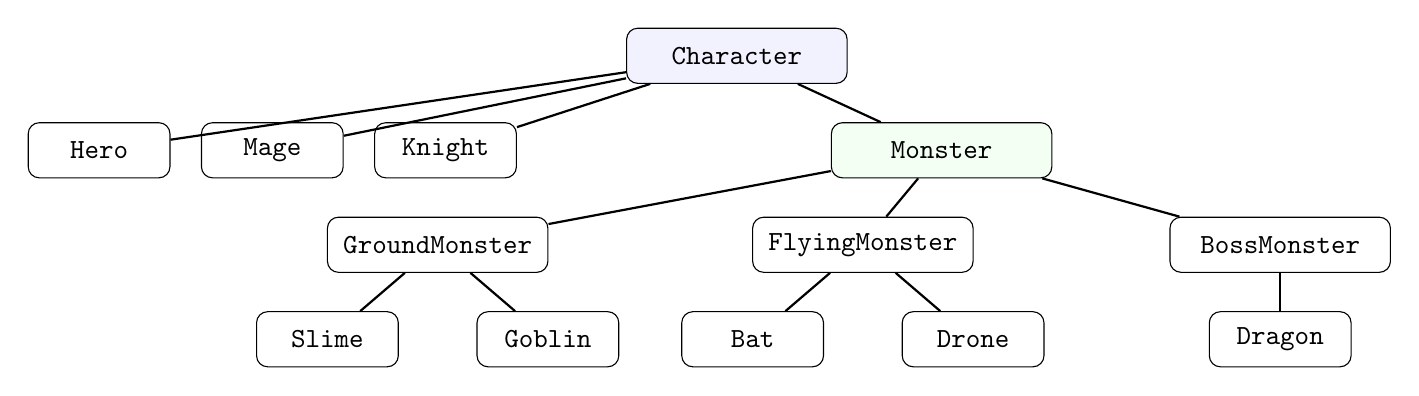
\begin{tikzpicture}[
        rpgNode/.style={rectangle, draw, rounded corners, align=center, minimum width=28mm, minimum height=7mm},
        rpgLeafNode/.style={rectangle, draw, rounded corners, align=center, minimum width=18mm, minimum height=7mm},
        line/.style={thick}
    ]
        \node[rpgNode, fill=blue!5] (character) at (0, 0) {\texttt{Character}};
        \node[rpgLeafNode] (hero) at (-8.1, -1.2) {\texttt{Hero}};
        \node[rpgLeafNode] (mage) at (-5.9, -1.2) {\texttt{Mage}};
        \node[rpgLeafNode] (knight) at (-3.7, -1.2) {\texttt{Knight}};
        \node[rpgNode, fill=green!5] (monster) at (2.6, -1.2) {\texttt{Monster}};
        \node[rpgNode] (ground) at (-3.8, -2.4) {\texttt{GroundMonster}};
        \node[rpgNode] (flying) at (1.6, -2.4) {\texttt{FlyingMonster}};
        \node[rpgNode] (boss) at (6.9, -2.4) {\texttt{BossMonster}};
        \node[rpgLeafNode] (slime) at (-5.2, -3.6) {\texttt{Slime}};
        \node[rpgLeafNode] (goblin) at (-2.4, -3.6) {\texttt{Goblin}};
        \node[rpgLeafNode] (bat) at (0.2, -3.6) {\texttt{Bat}};
        \node[rpgLeafNode] (drone) at (3.0, -3.6) {\texttt{Drone}};
        \node[rpgLeafNode] (dragon) at (6.9, -3.6) {\texttt{Dragon}};

        \draw[line] (character) -- (hero);
        \draw[line] (character) -- (mage);
        \draw[line] (character) -- (knight);
        \draw[line] (character) -- (monster);
        \draw[line] (monster) -- (ground);
        \draw[line] (monster) -- (flying);
        \draw[line] (monster) -- (boss);
        \draw[line] (ground) -- (slime);
        \draw[line] (ground) -- (goblin);
        \draw[line] (flying) -- (bat);
        \draw[line] (flying) -- (drone);
        \draw[line] (boss) -- (dragon);
    \end{tikzpicture}
    }
    \caption{RPG風キャラクターの継承関係}
    \label{fig:chapter14-rpg-inheritance-tree}
\end{figure}

この例では、\texttt{Character}に共通の情報を持たせます。そこから、味方キャラクターやモンスターを表す子クラスを作ります。\texttt{attack}、\texttt{magic}、\texttt{heal}は同じ名前のメソッドとして用意し、クラスごとに中身を変えます。

\begin{listing}[htbp]
\inputminted[firstline=1,lastline=45]{ts}{listings/chapter14/rpg-characters.ts}
\caption{共通部分を持つ\texttt{Character}クラス}
\label{lst:chapter14-rpg-character-base}
\end{listing}

\begin{listing}[htbp]
\inputminted[firstline=48,lastline=78]{ts}{listings/chapter14/rpg-characters.ts}
\caption{味方キャラクターと基本のモンスター}
\label{lst:chapter14-rpg-hero-monster}
\end{listing}

\begin{listing}[htbp]
\inputminted[firstline=80,lastline=114]{ts}{listings/chapter14/rpg-characters.ts}
\caption{地上と空中で分かれるモンスター}
\label{lst:chapter14-rpg-ground-flying-monsters}
\end{listing}

\begin{listing}[htbp]
\inputminted[firstline=116,lastline=130]{ts}{listings/chapter14/rpg-characters.ts}
\caption{ボスモンスターとドラゴン}
\label{lst:chapter14-rpg-boss-monster}
\end{listing}

\begin{listing}[htbp]
\inputminted[firstline=132,lastline=179]{ts}{listings/chapter14/rpg-characters.ts}
\caption{RPG風キャラクターを画面に表示する}
\label{lst:chapter14-rpg-sketch}
\end{listing}

\texttt{characters}は\texttt{Character[]}型の配列です。その中に\texttt{Hero}、\texttt{Mage}、\texttt{Knight}、\texttt{Slime}、\texttt{Dragon}などをまとめて入れています。どのクラスも\texttt{Character}をもとにしているため、同じ配列に入れられます。

\begin{pointbox}{共通の型でまとめ、違う行動を呼び出す}
\texttt{characters[0].attack()}と\texttt{characters[7].attack()}は同じ名前のメソッド呼び出しです。しかし、\texttt{Hero}なら剣で攻撃し、\texttt{Dragon}なら炎の息を吐きます。同じ呼び方で、インスタンスごとに違う行動をさせられるのが継承の面白いところです。
\end{pointbox}

\section{継承を使いすぎない}

継承は便利ですが、何でも継承にすればよいわけではありません。共通部分がはっきりしていて、「子クラスは親クラスの一種である」と自然に言えるときに使うと分かりやすくなります。

\begin{center}
\begin{tabular}{ll}
\toprule
考え方 & 例 \\
\midrule
使いやすい継承 & \texttt{FallingCircle}は\texttt{FallingShape}の一種 \\
分かりにくい継承 & \texttt{Player}は\texttt{Score}の一種 \\
\bottomrule
\end{tabular}
\end{center}

共通する処理が少ない場合や、親子関係として読むと不自然な場合は、無理に継承を使わなくてもかまいません。第11章のように別々のクラスとして書いた方が読みやすいこともあります。

\begin{notebox}{継承は設計の選択肢の1つ}
継承は、似たクラスを整理するための選択肢です。必ず使うものではありません。初学者の段階では、「共通部分を親クラスに置く」「違う部分を子クラスに置く」と読める場合に使う、くらいで十分です。
\end{notebox}

\begin{notebox}{\texttt{draw}という名前を避ける}
p5.jsの\texttt{p.draw}と区別しやすいように、図形クラスの描画メソッドは\texttt{display}と名付けます。
\end{notebox}

\section{よくある間違い}

継承では、親クラスと子クラスのどちらに何を書くのかが重要です。エラーが出たときは、\texttt{extends}の向き、\texttt{super}の呼び出し、メソッド名の一致を確認しましょう。

\begin{mistakebox}{\texttt{extends}の向きを逆にする}
\texttt{class JitteringSquare extends JitteringDot}は、「\texttt{JitteringSquare}は\texttt{JitteringDot}をもとにする」という意味です。親クラスと子クラスの順番を逆にしないようにしましょう。
\end{mistakebox}

\begin{mistakebox}{\texttt{super}を書き忘れる}
子クラスにコンストラクタを書く場合、基本的には最初に\texttt{super(...)}を呼びます。親クラスが持つフィールドの初期化を忘れないためです。
\end{mistakebox}

\begin{mistakebox}{メソッド名を少しだけ変えてしまう}
親クラスの\texttt{display}を上書きしたいのに、子クラスで\texttt{drawDisplay}のような別名を書いてしまうと、上書きにはなりません。同じ名前、同じ使い方で書くことを確認しましょう。
\end{mistakebox}

\begin{mistakebox}{親クラスにないメソッドを親クラス型の配列から呼ぶ}
\texttt{FallingShape[]}の配列から呼べるのは、\texttt{FallingShape}に定義されているメソッドです。子クラスだけが持つ特別なメソッドを呼びたい場合は、設計を見直す必要があります。
\end{mistakebox}

\begin{mistakebox}{継承で無理にまとめすぎる}
似ていないクラスを無理に親子関係にすると、かえって読みにくくなります。共通するフィールドやメソッドが少ない場合は、別々のクラスとして書く方が分かりやすいこともあります。
\end{mistakebox}

\section{まとめ}

この章では、継承を使って、あるクラスをもとに別のクラスを作る方法を学びました。\texttt{extends}を使うと親クラスのフィールドやメソッドを引き継げます。子クラスのコンストラクタでは\texttt{super}を使って親クラスのコンストラクタを呼び出します。

また、子クラスでは親クラスと同じ名前のメソッドを書いて処理を上書きできます。これにより、動き方は共通で、描き方だけが違う図形を作れます。親クラス型の配列を使うと、円や正方形のような異なる子クラスのインスタンスをまとめて扱えます。

RPG風の例では、\texttt{Character}にHP、名前、座標をまとめ、\texttt{Hero}や\texttt{Dragon}などの子クラスで\texttt{attack}、\texttt{magic}、\texttt{heal}の違いを表しました。継承は、画面上の図形だけでなく、ゲームに登場する役割や行動を整理するときにも使えます。

\section{演習問題}

この章の演習では、まず継承の書き方を確認し、次に子クラスのフィールドやメソッドを少しずつ変更していきます。最後は、第11章で作ったクラスを継承で整理する課題に進みます。

\begin{enumerate}
    \item \texttt{jittering-dot.ts}で、点が動く範囲を\texttt{p.random(-3, 3)}に変更してください。
    \item \texttt{jittering-square-inheritance.ts}で、\texttt{sideLength}を変えて正方形の大きさを変更してください。
    \item \texttt{JitteringSquare}の\texttt{display}メソッドで、正方形の色を変更してください。
    \item \texttt{jittering-mixed-array.ts}で、\texttt{things}に\texttt{JitteringSquare}をもう1つ追加してください。
    \item \texttt{FallingSquare}の\texttt{display}を変更し、正方形ではなく長方形を描く子クラスを作ってください。
    \item \texttt{FallingCircle}に、円の周りに外枠を太く描く処理を追加してください。
    \item \texttt{falling-shapes-inheritance.ts}で、図形の数を増やし、円と正方形の割合を変えてください。
    \item \texttt{ClickableSquare}の\texttt{display}を変更し、マウスが重なったときだけ大きく表示してください。
    \item \texttt{FallingShape}を継承する\texttt{FallingTriangle}クラスを作り、三角形が落ちるようにしてください。
    \item 第11章の\texttt{Ball}と\texttt{FallingSquare}を見直し、共通するフィールドとメソッドを\texttt{FallingShape}にまとめる案を説明してください。
    \item \texttt{rpg-characters.ts}で、\texttt{Healer}クラスを追加し、\texttt{heal}メソッドを上書きしてください。
    \item \texttt{rpg-characters.ts}で、\texttt{Monster}を継承する新しいモンスターを1種類追加してください。
    \item 挑戦問題として、親クラス\texttt{GameObject}を作り、プレイヤー、敵、アイテムを子クラスとして表す小さなデモを作ってください。
\end{enumerate}

\chapter{小さなゲームを作る}
\label{chap:small-game}

この章では、これまでに学んだ図形、色、変数、条件分岐、繰り返し、関数、配列、クラス、継承を組み合わせて、小さなゲームを作ります。ゲームは特別な命令だけで作るものではありません。画面を毎回描き直し、入力を読み取り、状態を少しずつ変え、条件に応じて得点やライフを更新することで作れます。

\section{この章の概要}

この章では、プレイヤーを動かして星を集め、落ちてくる敵を避ける「星集めゲーム」を作ります。最初から完成形を書くのではなく、まずプレイヤーを動かし、次に星を取る処理を加え、最後に敵、ライフ、ゲームオーバーを組み込みます。

この章で扱う主な内容は次の通りです。

\begin{itemize}
    \item ゲームを状態とルールに分けて考える
    \item キーボードでプレイヤーを動かす
    \item 当たり判定で得点を増やす
    \item 敵を配列で管理する
    \item ライフとゲームオーバーを扱う
    \item 関数でゲーム全体の処理を整理する
    \item 継承でプレイヤー、星、敵の共通部分をまとめる
    \item 押し続ける入力と押した瞬間の入力を使い分ける
\end{itemize}

\section{ゲームを状態とルールに分ける}

ゲームを作るときは、まず「何を覚えておく必要があるか」と「何が起きたら何を変えるか」を分けて考えると整理しやすくなります。画面に見えているものは、ほとんどの場合、変数やオブジェクトの状態を描いた結果です。

\begin{center}
\begin{tabular}{ll}
\toprule
考えること & この章のゲームでの例 \\
\midrule
状態 & プレイヤーの位置、星の位置、敵の位置、得点、ライフ \\
入力 & 矢印キーでプレイヤーを動かす \\
ルール & 星に触れたら得点、敵に触れたらライフを減らす \\
終了条件 & ライフが0になったらゲームオーバー \\
\bottomrule
\end{tabular}
\end{center}

\begin{pointbox}{ゲームは毎フレームの小さな判断で動く}
ゲームは、1回の大きな処理で完成するものではありません。\texttt{draw}が呼ばれるたびに、入力を見て、位置を更新し、当たり判定を行い、画面を描き直します。この小さな流れを何度も繰り返すことで、ゲームとして動いて見えます。
\end{pointbox}

\section{プレイヤーを動かす}

最初に、矢印キーで動くプレイヤーを作ります。プレイヤーは、中心座標、半径、移動速度を持つクラスとして表します。第11章で学んだように、プレイヤーに関する状態と処理を\texttt{Player}クラスにまとめます。

\begin{listing}[htbp]
\inputminted[firstline=1,lastline=44]{ts}{listings/chapter15/player-control.ts}
\caption{矢印キーで動く\texttt{Player}クラス}
\label{lst:chapter15-player-control-class}
\end{listing}

\begin{listing}[htbp]
\inputminted[firstline=46,lastline=62]{ts}{listings/chapter15/player-control.ts}
\caption{\texttt{Player}クラスを使うスケッチ}
\label{lst:chapter15-player-control-sketch}
\end{listing}

\texttt{Player}クラスの\texttt{update}メソッドでは、\texttt{p.keyIsDown}を使ってキーが押されているかを調べています。\texttt{update}は\texttt{draw}から毎フレーム呼ばれるため、\texttt{p.keyIsDown(p.LEFT\_ARROW)}のように押されている間の状態を調べると、キーを押し続けてプレイヤーを動かせます。左矢印キーが押されていればx座標を減らし、右矢印キーが押されていればx座標を増やします。上下方向も同じ考え方です。

\texttt{p.constrain}は、値を指定した範囲におさめる関数です。このサンプルでは、プレイヤーがキャンバスの外へ出ないように、\texttt{centerX}と\texttt{centerY}を制限しています。ゲームでは、動かすだけでなく、動いてよい範囲を決めることも大切です。

\section{星を取ったら得点を増やす}

次に、プレイヤーが星に触れたら得点が増えるようにします。星も、中心座標と半径を持つものとして考えられます。プレイヤーと星の距離を調べ、その距離が2つの半径の合計より小さければ、触れていると判断します。

\begin{figure}[htbp]
    \centering
    \begin{tikzpicture}[
        circleNode/.style={circle, draw, minimum size=20mm, align=center},
        arrow/.style={<->, thick}
    ]
        \node[circleNode, fill=blue!8] (player) at (0, 0) {Player};
        \node[circleNode, fill=yellow!20] (star) at (4, 0.6) {Star};
        \draw[arrow] (player.center) -- (star.center);
        \node[align=center] at (2, -0.8) {中心同士の距離};
        \node[align=center] at (2, -1.6) {距離 < 半径の合計なら触れている};
    \end{tikzpicture}
    \caption{円同士の当たり判定}
    \label{fig:chapter15-circle-hit-test}
\end{figure}

\begin{listing}[htbp]
\inputminted[firstline=1,lastline=44]{ts}{listings/chapter15/collect-star.ts}
\caption{星を取るサンプルで使う\texttt{Player}}
\label{lst:chapter15-collect-star-player}
\end{listing}

\begin{listing}[htbp]
\inputminted[firstline=46,lastline=82]{ts}{listings/chapter15/collect-star.ts}
\caption{取る対象になる\texttt{Star}}
\label{lst:chapter15-collect-star-class}
\end{listing}

\begin{listing}[htbp]
\inputminted[firstline=84,lastline=120]{ts}{listings/chapter15/collect-star.ts}
\caption{星を取ったら得点を増やすスケッチ}
\label{lst:chapter15-collect-star-sketch}
\end{listing}

\texttt{Star}クラスには、星の位置をランダムに置き直す\texttt{reset}メソッドがあります。星を取ったときに新しい星を出したいので、位置を決め直す処理をメソッドとしてまとめています。

\texttt{isTouching}メソッドは、プレイヤーと星が触れているかを\texttt{boolean}で返します。\texttt{true}なら触れている、\texttt{false}なら触れていないという意味です。ゲームのルールを書くとき、\texttt{boolean}を返す関数やメソッドを作ると、\texttt{if}文の条件として読みやすく使えます。

\begin{pointbox}{当たり判定はゲームのルールを支える}
当たり判定は、見た目を描く処理ではありません。「触れたら得点」「触れたらダメージ」のようなルールを実行するための判断です。そのため、\texttt{display}とは分けて、\texttt{isTouching}のような名前のメソッドにすると読みやすくなります。
\end{pointbox}

\section{完成版の構成}

完成版では、プレイヤー、星、敵をクラスで表します。さらに、どれも「中心座標と半径を持ち、当たり判定に使える」という共通点があるため、第14章で学んだ継承を使って\texttt{GameObject}クラスに共通部分をまとめます。

\begin{figure}[htbp]
    \centering
    \begin{tikzpicture}[
        box/.style={rectangle, draw, rounded corners, align=center, minimum width=32mm, minimum height=9mm},
        arrow/.style={->, thick}
    ]
        \node[box, fill=blue!5] (gameObject) at (0, 0) {\texttt{GameObject}\\座標・半径・当たり判定};
        \node[box, fill=green!5] (player) at (-4, -1.7) {\texttt{Player}\\キー入力で動く};
        \node[box, fill=yellow!15] (star) at (0, -1.7) {\texttt{Star}\\取ると得点};
        \node[box, fill=red!8] (enemy) at (4, -1.7) {\texttt{Enemy}\\落ちてくる};
        \draw[arrow] (player.north) -- (gameObject.south);
        \draw[arrow] (star.north) -- (gameObject.south);
        \draw[arrow] (enemy.north) -- (gameObject.south);
    \end{tikzpicture}
    \caption{完成版ゲームのクラス構成}
    \label{fig:chapter15-game-classes}
\end{figure}

\texttt{GameObject}は画面に登場するものの共通部分です。プレイヤーも星も敵も、中心座標と半径を持っています。また、どれも当たり判定では同じ計算を使えます。そこで、\texttt{isTouching}を親クラスに置き、子クラスから共通して使えるようにします。

\section{共通部分を\texttt{GameObject}にまとめる}

まず、完成版の親クラスを見ます。\texttt{GameObject}には、中心座標、半径、当たり判定だけを入れます。どのように描くか、どのように動くかは、子クラスごとに違うため、ここには入れません。

\begin{listing}[htbp]
\inputminted[firstline=1,lastline=25]{ts}{listings/chapter15/star-catcher-game.ts}
\caption{ゲーム内のものに共通する\texttt{GameObject}}
\label{lst:chapter15-game-object}
\end{listing}

\texttt{isTouching}の引数は\texttt{other: GameObject}です。これは、「相手も\texttt{GameObject}をもとにしたものなら調べられる」という意味です。\texttt{Player}、\texttt{Star}、\texttt{Enemy}はすべて\texttt{GameObject}を継承するので、同じ\texttt{isTouching}で当たり判定できます。

\begin{notebox}{親クラスには本当に共通するものだけを置く}
\texttt{GameObject}に何でも入れると、かえって分かりにくくなります。このゲームでは、座標、半径、当たり判定は共通しています。一方、キー入力、ランダムな再配置、下方向への移動はクラスごとに違うため、それぞれの子クラスに書きます。
\end{notebox}

\section{\texttt{Player}、\texttt{Star}、\texttt{Enemy}を作る}

次に、ゲームに登場する3種類のクラスを作ります。\texttt{Player}はキー入力で動き、\texttt{Star}は取られたら別の場所へ移動し、\texttt{Enemy}は上から下へ落ちてきます。同じ\texttt{GameObject}を継承していても、役割が違うため、持つメソッドも少しずつ違います。

\begin{listing}[htbp]
\inputminted[firstline=27,lastline=67]{ts}{listings/chapter15/star-catcher-game.ts}
\caption{キー入力で動く\texttt{Player}}
\label{lst:chapter15-player-class}
\end{listing}

\begin{listing}[htbp]
\inputminted[firstline=69,lastline=85]{ts}{listings/chapter15/star-catcher-game.ts}
\caption{集める対象になる\texttt{Star}}
\label{lst:chapter15-star-class}
\end{listing}

\begin{listing}[htbp]
\inputminted[firstline=87,lastline=116]{ts}{listings/chapter15/star-catcher-game.ts}
\caption{上から落ちてくる\texttt{Enemy}}
\label{lst:chapter15-enemy-class}
\end{listing}

\texttt{Player}の\texttt{update}は、矢印キーを調べて座標を変えます。\texttt{Star}の\texttt{reset}は、星をランダムな位置に置き直します。\texttt{Enemy}の\texttt{update}は、敵を下へ動かし、画面外に出たら上に戻します。

同じ\texttt{update}という名前でも、クラスごとに意味が少し違います。これは、第14章で学んだ「同じ名前のメソッドをクラスごとに用意する」という考え方につながります。このゲームでは、\texttt{Player}と\texttt{Enemy}がそれぞれ自分に必要な更新処理を持っています。

\section{ゲーム全体の状態を用意する}

クラスは、ゲームに登場するものを整理するために使います。一方で、得点、ライフ、ゲームオーバーかどうかのように、ゲーム全体で1つだけ持てばよい状態もあります。そのような値は、スケッチの中の変数として用意します。

\begin{listing}[htbp]
\inputminted[firstline=119,lastline=145]{ts}{listings/chapter15/star-catcher-game.ts}
\caption{ゲーム全体の状態を用意する}
\label{lst:chapter15-game-state}
\end{listing}

\texttt{score}は現在の得点、\texttt{life}は残りライフ、\texttt{isGameOver}はゲームオーバーかどうかを表します。\texttt{isGameOver}の型は\texttt{boolean}です。ゲームの状態を\texttt{true}または\texttt{false}で表すと、\texttt{if (isGameOver)}のように条件分岐で使いやすくなります。

\texttt{enemies}は\texttt{Enemy[]}型の配列です。敵は複数登場するため、1つずつ別の変数にするのではなく、配列にまとめています。第10章の配列、第11章のクラス、第14章の継承がここで一緒に使われています。

\section{\texttt{draw}でゲームを進める}

ゲームの中心になるのは\texttt{p.draw}です。\texttt{draw}の中では、まずゲームオーバーかどうかを調べます。ゲーム中なら、プレイヤーと敵を更新し、星や敵との当たり判定を行い、最後に画面を描きます。

\begin{listing}[htbp]
\inputminted[firstline=146,lastline=173]{ts}{listings/chapter15/star-catcher-game.ts}
\caption{\texttt{draw}でゲームのルールを進める}
\label{lst:chapter15-draw-rules}
\end{listing}

\texttt{if (star.isTouching(player, p))}は、星とプレイヤーが触れているかを調べています。触れていれば、\texttt{score}を1増やし、星を別の場所へ移動します。

敵との当たり判定は、敵の配列を\texttt{for}文で順番に調べます。どの敵に触れても、ライフを1減らし、その敵を上へ戻します。敵が複数いても、配列と繰り返しを使えば、同じ処理を1つの形で書けます。

\begin{mistakebox}{状態を変える場所を散らばらせすぎない}
得点やライフをいろいろな関数でばらばらに変更すると、どこで値が変わったのか分かりにくくなります。この章では、得点とライフの更新を\texttt{draw}のルール部分に集めています。
\end{mistakebox}

\section{ゲームオーバーと再スタート}

ライフが0になったら、\texttt{isGameOver}を\texttt{true}にします。次の\texttt{draw}では、ゲーム中の更新を行わず、ゲームオーバー画面だけを表示します。スペースキーが押されたら、得点とライフを初期値に戻し、敵と星の位置をリセットします。

\begin{listing}[htbp]
\inputminted[firstline=175,lastline=187]{ts}{listings/chapter15/star-catcher-game.ts}
\caption{スペースキーでゲームを再スタートする}
\label{lst:chapter15-restart}
\end{listing}

\texttt{p.keyPressed}は、キーが押された瞬間に1回呼ばれる処理です。プレイヤーの移動では、押され続けているキーを毎フレーム調べるために\texttt{p.keyIsDown}を使いました。一方、ゲームオーバーからの再スタートは、キーを押した瞬間に1回だけ実行したいので、\texttt{p.keyPressed}を使っています。このように、連続して変えたい状態には\texttt{p.keyIsDown}、一度だけ始めたい処理には\texttt{p.keyPressed}を使います。

\section{処理を関数に分ける}

完成版の最後では、ゲームを更新する処理、描画する処理、ステータス表示、ゲームオーバー表示を関数に分けています。関数に分けることで、\texttt{draw}の中で「今どの段階の処理をしているか」が読み取りやすくなります。

\begin{listing}[htbp]
\inputminted[firstline=190,lastline=237]{ts}{listings/chapter15/star-catcher-game.ts}
\caption{更新、描画、表示を関数に分ける}
\label{lst:chapter15-helper-functions}
\end{listing}

\texttt{updateGame}は、プレイヤーと敵の位置を更新します。\texttt{displayGame}は、星、敵、プレイヤー、得点、ライフを描画します。\texttt{displayStatus}と\texttt{displayGameOver}は、文字表示を担当します。

関数に分けるときは、何でも細かく分ければよいわけではありません。この章では、「更新」「描画」「状態表示」のように、役割で分けています。関数名を読むだけで、その関数がゲームのどの部分を担当しているか分かることが大切です。

\begin{pointbox}{完成版を読む順番}
長いプログラムは、上から1行ずつ読むだけでは大変です。まず、\texttt{setup}で何を作っているかを見ます。次に、\texttt{draw}で毎フレーム何をしているかを読みます。その後で、クラスや関数の中身を必要に応じて確認すると、全体像をつかみやすくなります。
\end{pointbox}

\section{よくある間違い}

小さなゲームでも、状態、入力、当たり判定、描画が組み合わさるため、間違いの原因が見つけにくくなることがあります。次の点を確認しながら作ると、原因を切り分けやすくなります。

\begin{mistakebox}{\texttt{draw}の中で毎回インスタンスを作ってしまう}
\texttt{draw}の中で\texttt{player = new Player(...)}のように書くと、毎フレーム位置が初期値に戻ってしまいます。インスタンスを作る処理は基本的に\texttt{setup}で行い、\texttt{draw}では状態を更新します。
\end{mistakebox}

\begin{mistakebox}{当たり判定と描画を混ぜてしまう}
\texttt{display}の中で得点を増やすと、「描く処理」と「ゲームのルール」が混ざってしまいます。表示する処理と、得点やライフを変える処理は分けて考えましょう。
\end{mistakebox}

\begin{mistakebox}{キー入力を使い分けられない}
押され続けている間プレイヤーを動かすなら\texttt{p.keyIsDown}を使います。ゲームオーバーからの再スタートのように、押した瞬間だけ実行したい処理には\texttt{p.keyPressed}を使います。
\end{mistakebox}

\begin{mistakebox}{配列の要素数と繰り返し条件をずらしてしまう}
敵の配列を処理するときは、\texttt{index < enemies.length}のように配列の長さを使います。固定の数値を書くと、敵の数を変えたときに修正忘れが起きやすくなります。
\end{mistakebox}

\begin{mistakebox}{ゲームオーバー中にも更新し続けてしまう}
ゲームオーバー画面を表示していても、敵やプレイヤーを更新し続けると、再スタート時に予想しない状態になりやすくなります。この章では、\texttt{isGameOver}が\texttt{true}なら早めに\texttt{return}して、ゲーム中の更新を止めています。
\end{mistakebox}

\section{まとめ}

この章では、これまで学んだ内容を組み合わせて、小さなゲームを作りました。ゲームでは、状態を変数やインスタンスに保存し、\texttt{draw}の中で少しずつ更新します。入力、当たり判定、得点、ライフ、ゲームオーバーは、すべて条件分岐や関数、クラスを使って表せます。

完成版では、\texttt{GameObject}を親クラスにして、\texttt{Player}、\texttt{Star}、\texttt{Enemy}の共通部分をまとめました。継承を使うことで、当たり判定を1か所に置き、種類ごとの違いは子クラスに書けます。小さなゲームを作ることは、プログラムの部品をどう分けるかを考える練習にもなります。

\section{演習問題}

この章の演習では、まず完成版の値を少し変え、次にルールやクラスを追加していきます。最後は、自分なりの小さなゲームへ発展させます。

\begin{enumerate}
    \item \texttt{player-control.ts}で、プレイヤーの移動速度を変えて、操作感がどう変わるか確認してください。
    \item \texttt{collect-star.ts}で、星の半径を大きくし、取りやすさがどう変わるか確認してください。
    \item \texttt{star-catcher-game.ts}で、敵の数を\texttt{4}から\texttt{6}に変更してください。
    \item \texttt{Enemy}の\texttt{speedY}の範囲を変更し、敵の落ちる速さを調整してください。
    \item 星を取ったときに、得点が2点増えるように変更してください。
    \item 敵に当たったときに、ライフが減るだけでなく、プレイヤーの位置も初期位置に戻るようにしてください。
    \item \texttt{Star}をもう1つ増やし、2つの星を集められるようにしてください。
    \item 新しい子クラス\texttt{BonusStar}を作り、取ると得点が5点増えるようにしてください。
    \item 敵に当たった直後、少しの間だけ連続でライフが減らない仕組みを考えてください。
    \item 自由制作として、プレイヤー、集めるもの、避けるものを変え、自分なりの小さなゲームを作ってください。
    \item 挑戦問題として、ゲームクリア条件を追加してください。たとえば、得点が20点になったらクリア画面を表示するようにします。
\end{enumerate}

\chapter{ファイル入出力}
\label{chap:file-io}

この章では、ゲームに必要な設定を外部ファイルから読み込み、得点のように残しておきたい値を保存する方法を学びます。ここで扱うファイル入出力は、ゲームの初期設定、難易度調整、最高得点の記録など、実際の制作で使いやすい場面にしぼって考えます。

\section{この章の概要}

前の章では、小さなゲームを1つのプログラムとして作りました。しかし、ゲームが少し大きくなると、キャンバスの大きさ、プレイヤーの速さ、敵の速さ、得点の増え方などを、プログラムの中に直接書き続けるのが大変になります。p5.jsはブラウザの中で動くため、プログラムからコンピュータ上のファイルを自由に書き換えることはできません。この章では、設定をJSONファイルから読み込み、最高得点をブラウザの保存領域に保存します。

この章で扱う主な内容は次の通りです。

\begin{itemize}
    \item ブラウザでの読み込みと保存の違いを理解する
    \item JSONの基本的な書き方を知る
    \item JSONファイルにゲームの初期設定を書く
    \item \texttt{async setup}と\texttt{await}で設定ファイルを読み込む
    \item 読み込んだ設定をクラスで扱いやすくする
    \item \texttt{storeItem}と\texttt{getItem}で最高得点を保存する
    \item 設定読み込みと得点保存を小さなゲームに組み込む
\end{itemize}

\section{ゲーム設定を外に出す}

ゲームの調整値をプログラムの外に出すと、コードを大きく書き換えずに難易度を変えられます。たとえば、プレイヤーの速度だけを少し上げたいとき、TypeScriptのクラスや関数を探して変更するより、設定ファイルの数値を変える方が分かりやすい場合があります。

この章では、JSONという形式で設定を書きます。JSONは、名前と値の組を並べてデータを表す形式です。Webアプリ、ゲーム、サーバとの通信、設定ファイルなど、さまざまな場面で使われています。今後プログラムを作るときにも何度も出会う形式なので、ここで基本を確認しておきます。

\section{JSONの基本}

JSONは、データを文字として保存したり、別のプログラムに渡したりするための書き方です。見た目はTypeScriptのオブジェクトに似ていますが、JSONは「プログラムそのもの」ではなく「データを表すための形式」です。

JSONでは、全体を\texttt{\{}と\texttt{\}}で囲みます。その中に、\texttt{"名前": 値}という組を並べます。名前は必ずダブルクォーテーション\texttt{" "}で囲みます。複数の項目を書くときは、項目の間をカンマで区切ります。

\begin{listing}[htbp]
\begin{minted}{json}
{
    "playerSpeed": 5,
    "startLife": 3,
    "gameTitle": "Star Catcher",
    "showGrid": false
}
\end{minted}
\caption{JSONの基本的な書き方}
\label{lst:chapter16-json-basic}
\end{listing}

この例では、\texttt{playerSpeed}、\texttt{startLife}、\texttt{gameTitle}、\texttt{showGrid}が名前です。それぞれの右側にある\texttt{5}、\texttt{3}、\texttt{"Star Catcher"}、\texttt{false}が値です。

\begin{center}
\begin{tabular}{lll}
\toprule
JSONの値 & TypeScriptで考える型 & 例 \\
\midrule
数値 & \texttt{number} & \texttt{5}, \texttt{3.5} \\
文字列 & \texttt{string} & \texttt{"Star Catcher"} \\
真偽値 & \texttt{boolean} & \texttt{true}, \texttt{false} \\
配列 & 配列 & \texttt{[1, 2, 3]} \\
オブジェクト & オブジェクト & \texttt{\{"x": 100, "y": 80\}} \\
\bottomrule
\end{tabular}
\end{center}

TypeScriptで使う\texttt{number}、\texttt{string}、\texttt{boolean}という考え方は、JSONを読むときにも役に立ちます。たとえば、\texttt{"playerSpeed": 5}なら、\texttt{playerSpeed}は数値として使えます。一方、\texttt{"playerSpeed": "5"}のようにダブルクォーテーションで囲むと、見た目は数字でも文字列として扱われます。

\begin{pointbox}{JSONは設定を共有しやすい}
JSONは、TypeScriptだけでなく多くの言語やツールで読めます。そのため、ゲームの設定、Webサービスのデータ、エディタの設定など、プログラムの外に置きたいデータによく使われます。
\end{pointbox}

\section{JSONとTypeScriptオブジェクトの違い}

JSONはTypeScriptのオブジェクトに似ていますが、同じものではありません。TypeScriptのオブジェクトはプログラムの中で直接使う値です。一方、JSONはファイルや通信でやり取りするためのデータ形式です。

\begin{center}
\begin{tabular}{lll}
\toprule
内容 & JSON & TypeScriptオブジェクト \\
\midrule
名前の書き方 & \texttt{"playerSpeed"} & \texttt{playerSpeed}も使える \\
文字列 & ダブルクォーテーションのみ & シングルクォートも使える \\
コメント & 書けない & 書ける \\
最後のカンマ & 書かない & 書ける場合がある \\
関数 & 書けない & メソッドとして書ける \\
\bottomrule
\end{tabular}
\end{center}

特に間違えやすいのは、JSONにはコメントを書けないという点です。TypeScriptでは\texttt{// プレイヤーの速さ}のようなコメントを書けますが、JSONファイルの中に同じように書くと読み込みに失敗します。設定の説明を書きたい場合は、教材やREADMEに説明を書くか、名前そのものを\texttt{playerSpeed}のように分かりやすくします。

\begin{mistakebox}{JSONでよくある書き間違い}
名前をダブルクォーテーションで囲み忘れる、項目の間のカンマを忘れる、最後の項目のあとに余計なカンマを書く、といった間違いがよくあります。JSONは書き方に厳しいので、1文字の違いで読み込めなくなることがあります。
\end{mistakebox}

\section{ゲーム設定をJSONで書く}

それでは、実際にゲームの設定をJSONファイルに書いてみます。ここでは、キャンバスの大きさ、プレイヤーの速さ、敵の速さ、星を取ったときの得点、開始時のライフを設定として外に出します。

\begin{listing}[htbp]
\inputminted{json}{listings/chapter16/game-settings.json}
\caption{ゲームの初期設定を書くJSONファイル}
\label{lst:chapter16-game-settings-json}
\end{listing}

このファイルは、実際のp5.jsプロジェクトでは\texttt{public/data/game-settings.json}のような場所に置くことを想定します。プログラムからは\texttt{"data/game-settings.json"}というパスで読み込みます。

\begin{pointbox}{設定ファイルに向いている値}
キャンバスの大きさ、敵の速さ、開始時のライフ、得点の増え方のように、ゲームの調整で変えたくなる値は設定ファイルに向いています。一方、当たり判定の計算やキー入力の処理のようなルールそのものは、TypeScriptのコードに書きます。
\end{pointbox}

\section{\texttt{async setup}で設定を読み込む}

p5.js 2の\texttt{p.loadJSON}は、読み込みの完了をあとから知らせる\texttt{Promise}を返します。そのため、第\ref{chap:images-and-text}章で画像を読み込んだときと同じように、\texttt{p.setup}へ\texttt{async}を付け、\texttt{await p.loadJSON(...)}で読み込みが終わるのを待ちます。設定を受け取ってから\texttt{createCanvas}を呼べば、JSONに書いた大きさでキャンバスを作れます。

\texttt{async}は、関数の中で\texttt{await}を使えるようにする指定です。\texttt{await}は、\texttt{Promise}が完了して読み込んだ値を受け取るまで、次の行へ進まないようにします。\texttt{p.setup = async (): Promise<void> => \{ ... \};}の\texttt{Promise<void>}は、「処理はあとで完了し、完了時に値を返さない」という戻り値の型です。

\begin{listing}[htbp]
\inputminted[firstline=1,lastline=39]{ts}{listings/chapter16/load-settings.ts}
\caption{設定値をまとめる\texttt{GameSettings}クラス}
\label{lst:chapter16-game-settings-class}
\end{listing}

\begin{listing}[htbp]
\inputminted[firstline=41,lastline=79]{ts}{listings/chapter16/load-settings.ts}
\caption{\texttt{async setup}でJSON設定を読み込む}
\label{lst:chapter16-load-settings}
\end{listing}

\texttt{GameSettings}クラスは、JSONから読み込んだ値をゲーム内で扱いやすくするためのクラスです。JSONのままでも値を読むことはできますが、クラスに入れると、\texttt{gameSettings.playerSpeed}のように意味のある名前で使えます。

\begin{figure}[htbp]
    \centering
    \begin{tikzpicture}[
        font=\small,
        flowbox/.style={draw, rounded corners=3pt, minimum width=38mm, minimum height=24mm, align=center},
        flowarrow/.style={->, thick}
    ]
        \node[flowbox, fill=yellow!10] (json) at (0,0)
            {JSONファイル\\
             \texttt{game-settings.json}\\
             文字列として保存された設定};
        \node[flowbox, fill=blue!7] (settings) at (5.2,0)
            {\texttt{GameSettings}\\
             \texttt{playerSpeed}\\
             \texttt{enemySpeed}など};
        \node[flowbox, fill=green!8] (game) at (10.4,0)
            {ゲーム\\
             キャンバスの大きさ\\
             移動速度・得点・ライフ};

        \draw[flowarrow] (json) -- (settings);
        \draw[flowarrow] (settings) -- (game);
        \node[align=center, font=\scriptsize] at (2.6,1.65)
            {\texttt{await p.loadJSON(...)}\\で読み込む};
        \node[align=center, font=\scriptsize] at (7.8,1.65)
            {意味のある型と名前で\\ゲームから使う};
    \end{tikzpicture}
    \caption{JSONの設定を\texttt{GameSettings}へ入れてゲームで使う流れ}
    \label{fig:chapter16-json-settings-flow}
\end{figure}

図\ref{fig:chapter16-json-settings-flow}の左から右へ進むにつれて、ファイルに保存された設定が、TypeScriptのクラスを通してゲーム内で使える値になります。JSONファイルを書き換えると、TypeScriptのルール部分を変更せずに速度や得点を調整できます。

\texttt{p.loadJSON}は、JSONファイルを読み込むp5.jsの機能です。p5.js instance modeでは、\texttt{p.}を付けて\texttt{p.loadJSON}と書きます。\texttt{await}を付けると、\texttt{Promise}から読み込み済みのオブジェクトを受け取れます。

読み込んだオブジェクトには、TypeScriptから見ると「どのような形のデータか」がすぐには分かりません。そのため、\texttt{as \{ ... \}}の部分で、\texttt{canvasWidth}や\texttt{playerSpeed}などを持つデータとして扱うことを明示しています。この形を書くことで、設定ファイルにどの値が必要なのかも読み取りやすくなります。

\section{得点を保存する}

ゲームでは、プレイが終わったあとも最高得点を残しておきたいことがあります。ブラウザ版のp5.jsでは、\texttt{storeItem}と\texttt{getItem}を使うと、ブラウザの保存領域に小さな値を保存できます。

\begin{listing}[htbp]
\inputminted[firstline=1,lastline=27]{ts}{listings/chapter16/save-score.ts}
\caption{保存してある最高得点を読み込む}
\label{lst:chapter16-load-high-score}
\end{listing}

\begin{listing}[htbp]
\inputminted[firstline=29,lastline=57]{ts}{listings/chapter16/save-score.ts}
\caption{最高得点を保存・リセットする}
\label{lst:chapter16-save-high-score}
\end{listing}

\texttt{p.getItem("highScore")}は、\texttt{highScore}という名前で保存されている値を読み込みます。保存されていない場合もあるため、読み込んだ値が\texttt{number}かどうかを\texttt{typeof}で確認してから使っています。

\texttt{p.storeItem("highScore", highScore)}は、最高得点を保存します。この保存は、同じブラウザで同じページを開いたときに利用できます。別のコンピュータや別のブラウザには自動では引き継がれません。

\begin{figure}[htbp]
    \centering
    \begin{tikzpicture}[
        font=\small,
        flowbox/.style={draw, rounded corners=3pt, minimum width=39mm, minimum height=22mm, align=center},
        flowarrow/.style={->, thick}
    ]
        \node[flowbox, fill=orange!10] (score) at (0,0)
            {今回のゲーム\\\texttt{highScore = 120}};
        \node[flowbox, fill=blue!7] (storage) at (5.2,0)
            {ブラウザの保存領域\\\texttt{localStorage}\\キー: \texttt{highScore}};
        \node[flowbox, fill=green!8] (next) at (10.4,0)
            {次にページを開いたとき\\保存済みの最高得点を\\画面へ戻す};

        \draw[flowarrow] (score) -- (storage);
        \draw[flowarrow] (storage) -- (next);
        \node[align=center, font=\scriptsize] at (2.6,1.55)
            {\texttt{p.storeItem(...)}\\で保存};
        \node[align=center, font=\scriptsize] at (7.8,1.55)
            {\texttt{p.getItem(...)}\\で読み出す};
    \end{tikzpicture}
    \caption{最高得点を保存して次回の起動時に読み出す流れ}
    \label{fig:chapter16-score-storage-flow}
\end{figure}

図\ref{fig:chapter16-score-storage-flow}の保存先は、プロジェクト内のファイルではなく、ブラウザがページごとに持つ\texttt{localStorage}です。次に同じページを開いたとき、同じキー名を使って値を読み出します。

\begin{mistakebox}{保存したつもりでも保存場所が違うことがある}
\texttt{storeItem}の保存先はブラウザごとの保存領域です。ファイルとしてプロジェクトのフォルダに書き込まれるわけではありません。また、別のURLとして開くと、同じキー名でも別の保存先として扱われることがあります。
\end{mistakebox}

\section{設定と保存をゲームに組み込む}

ここまでの内容を組み合わせると、ゲームの初期設定をJSONから読み込み、ゲームオーバー時に最高得点を保存する小さなゲームを作れます。第15章の星集めゲームを少し簡単にし、ファイル入出力の役割が見えやすい形にします。

\begin{listing}[htbp]
\inputminted[firstline=1,lastline=39]{ts}{listings/chapter16/configurable-star-game.ts}
\caption{完成版で使う\texttt{GameSettings}}
\label{lst:chapter16-configurable-settings}
\end{listing}

\begin{listing}[htbp]
\inputminted[
    firstline=41,
    lastline=92,
    baselinestretch=0.95
]{ts}{listings/chapter16/configurable-star-game.ts}
\caption{設定された速度で動く\texttt{Player}}
\label{lst:chapter16-player-class}
\end{listing}

\begin{listing}[htbp]
\inputminted[firstline=94,lastline=133]{ts}{listings/chapter16/configurable-star-game.ts}
\caption{得点の対象になる\texttt{Star}}
\label{lst:chapter16-star-class}
\end{listing}

\begin{listing}[htbp]
\inputminted[firstline=135,lastline=179]{ts}{listings/chapter16/configurable-star-game.ts}
\caption{敵のクラス}
\label{lst:chapter16-enemy}
\end{listing}

\begin{listing}[htbp]
\inputminted[firstline=181,lastline=204]{ts}{listings/chapter16/configurable-star-game.ts}
\caption{ゲーム全体で使う変数}
\label{lst:chapter16-game-state}
\end{listing}

\begin{listing}[htbp]
\inputminted[firstline=206,lastline=250]{ts}{listings/chapter16/configurable-star-game.ts}
\caption{設定を読み込む\texttt{setup}とゲームの進行}
\label{lst:chapter16-setup-draw-key}
\end{listing}

\begin{listing}[htbp]
\inputminted[firstline=252,lastline=274]{ts}{listings/chapter16/configurable-star-game.ts}
\caption{設定を使ってゲームを更新する}
\label{lst:chapter16-update-game}
\end{listing}

\begin{listing}[htbp]
\inputminted[firstline=276,lastline=295]{ts}{listings/chapter16/configurable-star-game.ts}
\caption{ゲーム画面とゲームオーバー表示}
\label{lst:chapter16-display-game}
\end{listing}

\begin{listing}[htbp]
\inputminted[firstline=297,lastline=315]{ts}{listings/chapter16/configurable-star-game.ts}
\caption{再スタートと最高得点の保存}
\label{lst:chapter16-reset-and-save}
\end{listing}

この完成例では、\texttt{playerSpeed}、\texttt{enemySpeed}、\texttt{starScore}、\texttt{startLife}を設定ファイルから読み込みます。ゲームの難しさや得点の増え方は、コードではなくJSONの値を変えることで調整できます。

\texttt{updateGame}では、星を取ったときに\texttt{gameSettings.starScore}だけ得点を増やします。敵に触れてライフが0になったら\texttt{isGameOver}を\texttt{true}にし、\texttt{saveHighScore}を呼び出します。保存処理をゲームオーバーのタイミングにまとめることで、いつ得点が保存されるのかが分かりやすくなります。

\begin{pointbox}{設定と状態を分けて考える}
\texttt{gameSettings.startLife}は「ゲーム開始時の設定」です。一方、\texttt{life}は「今の残りライフ」です。設定値と現在の状態を同じ変数にしてしまうと、再スタートするときに元の値が分からなくなります。
\end{pointbox}

\section{JSONファイルを書き換えて調整する}

設定ファイルを使う良さは、ゲームを調整しやすくなることです。たとえば、敵が速すぎるなら\texttt{enemySpeed}を小さくします。ゲームが簡単すぎるなら、\texttt{startLife}を減らしたり、\texttt{enemySpeed}を大きくしたりできます。

\begin{center}
\begin{tabular}{lll}
\toprule
変えたいこと & 変更する設定 & 例 \\
\midrule
画面を広くする & \texttt{canvasWidth}, \texttt{canvasHeight} & \texttt{640}, \texttt{400} \\
プレイヤーを速くする & \texttt{playerSpeed} & \texttt{7} \\
敵を遅くする & \texttt{enemySpeed} & \texttt{2} \\
星の得点を増やす & \texttt{starScore} & \texttt{20} \\
ゲームを難しくする & \texttt{startLife} & \texttt{1} \\
\bottomrule
\end{tabular}
\end{center}

ただし、設定ファイルにどんな値でも入れてよいわけではありません。たとえば、\texttt{playerSpeed}を\texttt{0}にするとプレイヤーは動けなくなります。設定ファイルを使う場合も、どの範囲の値ならゲームとして成り立つかを考える必要があります。

\begin{pointbox}{ブラウザ版p5.jsでの保存の考え方}
ゲームの設定を使うときは、\texttt{p.loadJSON}でJSONファイルを読み込みます。最高得点のように小さな値を次回も使いたいときは、\texttt{p.storeItem}でブラウザの保存領域に残します。\texttt{p.saveJSON}を使うとJSONファイルをダウンロードできますが、プロジェクト内のファイルを直接書き換えるものではありません。
\end{pointbox}

\section{よくある間違い}

ファイル入出力では、コードが正しく見えても、ファイルの置き場所や読み込みのタイミングでつまずくことがあります。エラーが出たときは、変数の値だけでなく、ファイルのパスと実行環境も確認します。

\begin{mistakebox}{\texttt{await}せずに読み込んだ値を使おうとする}
\texttt{p.loadJSON}が返す\texttt{Promise}は、読み込み済みの設定そのものではありません。\texttt{async setup}の中で\texttt{await}を付け、設定を受け取ってから\texttt{GameSettings}やキャンバスを作ります。
\end{mistakebox}

\begin{mistakebox}{JSONの名前とTypeScript側の名前がずれている}
JSONに\texttt{player\_speed}と書き、TypeScript側で\texttt{playerSpeed}を読もうとしても、同じ値として扱われません。名前は1文字違っても別のものです。
\end{mistakebox}

\begin{mistakebox}{保存した得点が別の環境で見えない}
\texttt{storeItem}で保存した値は、基本的にそのブラウザの保存領域に残ります。別のブラウザ、別のコンピュータ、別のURLでは同じ得点が見えないことがあります。
\end{mistakebox}

\section{まとめ}

この章では、ゲームの初期設定をJSONファイルから読み込み、最高得点をブラウザに保存する方法を学びました。ファイル入出力を使うと、プログラムの中に直接書いていた調整値を外に出せます。また、プレイヤーの記録を次回の実行に残すこともできます。

JSONの読み込みには時間がかかるため、\texttt{p.setup}へ\texttt{async}を付け、\texttt{await p.loadJSON(...)}で完了を待ちます。読み込んだ設定を受け取ってから、キャンバスやゲームの状態を初期化します。

ブラウザで動くp5.jsでは、ローカルファイルを自由に書き換えることはできません。読み込み、保存、ダウンロードの違いを理解しておくと、ゲーム制作で何をどこに保存すればよいか判断しやすくなります。

\section{演習問題}

この章の演習では、設定ファイルの値を変えるところから始め、少しずつゲームの調整項目や保存する値を増やしていきます。

\begin{enumerate}
    \item \texttt{game-settings.json}の\texttt{playerSpeed}を変更し、プレイヤーの動きがどう変わるか確認しなさい。
    \item \texttt{enemySpeed}を変更し、ゲームの難易度がどう変わるか説明しなさい。
    \item \texttt{starScore}を\texttt{5}、\texttt{10}、\texttt{50}に変えて、得点の増え方を比べなさい。
    \item \texttt{startLife}を変更し、ゲームオーバーまでの長さがどう変わるか確認しなさい。
    \item JSONに\texttt{enemyRadius}を追加し、敵の半径を設定ファイルから変えられるようにしなさい。
    \item JSONに\texttt{playerRadius}を追加し、プレイヤーの大きさを設定できるようにしなさい。
    \item 最高得点だけでなく、最後に遊んだときの得点も保存して表示しなさい。
    \item \texttt{R}キーで最高得点をリセットする機能を、完成版のゲームにも追加しなさい。
    \item ゲームオーバー時に、\texttt{p.saveJSON}を使って得点をファイルとしてダウンロードする処理を調べ、試しなさい。
    \item 設定ファイルを「やさしい」「ふつう」「むずかしい」の3種類に分ける方法を考えなさい。
    \item 自分で小さなゲームを1つ作り、設定ファイルから少なくとも3つの値を読み込むようにしなさい。
\end{enumerate}

\chapter{音声を扱う}
\label{chap:sound}

この章では、TypeScript + p5.jsで音声ファイルを読み込み、再生、一時停止、繰り返し再生、効果音の再生を行う方法を学びます。前の章ではJSONファイルを読み込みました。音声ファイルも、画像やJSONと同じように、プログラムの外にある素材を読み込んで使います。

\section{この章の概要}

音声を使うと、ゲームやインタラクティブな作品の印象は大きく変わります。星を取ったときに短い効果音を鳴らしたり、ゲーム中に背景音楽を流したりすると、画面上の変化がより分かりやすくなります。

この章で扱う主な内容は次の通りです。

\begin{itemize}
    \item p5.soundを使う準備を知る
    \item \texttt{async setup}と\texttt{await}で音声ファイルを読み込む
    \item マウス操作をきっかけに音を鳴らす
    \item 再生、一時停止、停止、繰り返し再生を使い分ける
    \item ゲームの効果音として音声を組み込む
    \item 発振器で簡単な音を作る
    \item p5.soundで音声ファイルと波形を扱う
\end{itemize}

\begin{notebox}{音声ファイルについて}
この章のサンプルでは、\texttt{public/sounds/background.mp3}や\texttt{public/sounds/get-star.wav}のように、教材プロジェクトの公開用フォルダに音声ファイルを置くことを想定します。プログラムからは\texttt{"sounds/background.mp3"}のようなパスで読み込みます。
\end{notebox}

\begin{notebox}{教材テンプレートのp5.sound補助ファイル}
公式のp5.soundは、p5.js本体とは別のパッケージです。教材テンプレートにはp5.sound 0.3.0と、その機能を準備する\texttt{p5-sound} 補助ファイルが含まれています。各サンプルの\texttt{import "./p5-sound";}は、この補助ファイルを読み込む1行です。補助ファイルの中身を編集する必要はありません。
\end{notebox}

\section{p5.soundとブラウザの制約}

p5.soundは、p5.jsで音声を扱うための公式の追加ライブラリです。p5.soundを使うと、音声ファイルを読み込んだり、音を一時停止したり、簡単な波形を作ったりできます。サンプルでは、p5.jsのimportに加えて\texttt{import "./p5-sound";}を書き、音声機能の準備が終わってからスケッチを開始します。

ただし、ブラウザで動くプログラムには大切な制約があります。多くのブラウザでは、ページを開いただけで自動的に音を鳴らすことが制限されています。そのため、マウスクリックやキー入力など、ユーザーの操作をきっかけに音声を開始する必要があります。

この章のサンプルでは、p5.jsのインスタンスを受け取る変数名を\texttt{p5Instance}にしています。これまでの章で使ってきた\texttt{p}と役割は同じですが、音声のように新しい命令が増える章では、変数名から「p5.jsの機能をまとめたもの」だと分かるようにしています。

\begin{pointbox}{まずユーザー操作で音声を開始する}
p5.jsでは、\texttt{p5Instance.userStartAudio()}を呼ぶことで、ブラウザに「このページで音を出します」と伝えます。多くの場合、この処理は\texttt{p5Instance.mousePressed}や\texttt{p5Instance.keyPressed}の中で呼び出します。
\end{pointbox}

\section{音声ファイルを読み込んで再生する}

最初に、音声ファイルを1つ読み込み、マウスクリックで再生するサンプルを見ます。現在の\texttt{p5Instance.loadSound}は、音声ファイルの読み込み完了をあとから知らせる\texttt{Promise}を返します。そこで、前章のJSON読み込みと同じように、\texttt{p5Instance.setup}へ\texttt{async}を付け、\texttt{await}で読み込みが終わるのを待ちます。

\texttt{music = await p5Instance.loadSound(...)}と書くと、\texttt{Promise}から読み込み済みの\texttt{p5.SoundFile}を受け取れます。\texttt{Promise<void>}は、\texttt{setup}の処理があとで完了し、完了時に値を返さないことを表します。キャンバスは、音声の読み込みが終わったあとに作ります。

\begin{listing}[htbp]
\inputminted{ts}{listings/chapter17/play-sound.ts}
\caption{マウスクリックで音声を再生する}
\label{lst:chapter17-play-sound}
\end{listing}

\texttt{music: p5.SoundFile}は、読み込んだ音声ファイルを入れておく変数です。サンプルでは、\texttt{await}で受け取った音声ファイルを\texttt{music}に保存しています。\texttt{p5.SoundFile}に対して\texttt{play()}を呼ぶと再生し、\texttt{pause()}を呼ぶと一時停止し、\texttt{stop()}を呼ぶと停止します。

\texttt{p5Instance.mousePressed}の中では、最初に\texttt{p5Instance.userStartAudio()}を呼びます。その後で\texttt{music.play()}を呼ぶと、音声の再生が始まります。\texttt{isAudioStarted}は、音声を開始するための処理をすでに行ったかどうかを覚えておく変数です。

\section{再生操作を増やす}

音声を扱うときは、再生だけでなく、一時停止、停止、繰り返し再生もよく使います。ここでは、マウスクリックで先頭から再生し、キー操作で一時停止やループ再生を行うサンプルを作ります。

\begin{listing}[htbp]
\inputminted[firstline=1,lastline=33]{ts}{listings/chapter17/sound-controls.ts}
\caption{音声操作のための変数と画面表示}
\label{lst:chapter17-sound-controls-display}
\end{listing}

\begin{listing}[htbp]
\inputminted[firstline=35,lastline=65]{ts}{listings/chapter17/sound-controls.ts}
\caption{再生、一時停止、繰り返し、停止の操作}
\label{lst:chapter17-sound-controls-input}
\end{listing}

\texttt{music.isPlaying()}は、音声が現在再生中かどうかを調べ、再生中は\texttt{true}を、それ以外の場合は\texttt{false}を返します。

\texttt{music.play()}は現在位置から再生を始めます。クリックするたびに先頭から鳴らしたい場合は、先に\texttt{music.stop()}を呼び、その後で\texttt{music.play()}を呼びます。

\texttt{music.pause()}は一時停止です。もう一度\texttt{play()}を呼ぶと、止めた位置の続きから再生します。\texttt{music.stop()}は停止です。次に再生するときは、基本的に先頭から始まります。\texttt{music.loop()}は繰り返しを有効にします。停止中なら続けて\texttt{music.play()}を呼び、背景音楽のように同じ音を流し続けます。

\begin{figure}[H]
    \centering
    \begin{tikzpicture}[
        font=\small,
        state/.style={draw, rounded corners=4pt, minimum width=38mm, minimum height=17mm, align=center},
        transition/.style={->, thick}
    ]
        \node[state, fill=gray!10] (stopped) at (0,0)
            {停止中\\次は先頭から};
        \node[state, fill=green!10] (playing) at (8.0,0)
            {再生中\\再生位置が進む};
        \node[state, fill=yellow!13] (paused) at (8.0,-4.0)
            {一時停止中\\途中の位置を保持};

        \draw[transition] (stopped.east) --
            node[midway, below=2pt, align=center]{\texttt{play()}\\先頭から再生}
            (playing.west);
        \draw[transition] (playing.north west) to[bend right=32]
            node[above]{\texttt{stop()}または自然終了}
            (stopped.north east);
        \draw[transition] (playing.south east) to[bend left=18]
            node[right]{\texttt{pause()}}
            (paused.north east);
        \draw[transition] (paused.north west) to[bend left=18]
            node[left, align=right]{\texttt{play()}\\途中から再開}
            (playing.south west);
        \draw[transition] (paused.west) --
            node[midway, below left]{\texttt{stop()}}
            (stopped.south east);
    \end{tikzpicture}
    \caption{再生、一時停止、停止、再開による音声の状態変化}
    \label{fig:chapter17-sound-state-transition}
\end{figure}

図\ref{fig:chapter17-sound-state-transition}では、\texttt{pause()}と\texttt{stop()}の違いを状態として表しています。一時停止中は途中の再生位置を覚えているため、\texttt{play()}で続きから再開します。停止中から\texttt{play()}を呼ぶと、先頭から再生します。

\begin{notebox}{停止と一時停止は同じではない}
\texttt{pause()}は「途中で止めておく」操作です。\texttt{stop()}は「再生を止め、次は先頭から始める」操作として考えると分かりやすくなります。ゲームの効果音では、同じ音を何度も先頭から鳴らしたいことが多いため、\texttt{stop()}と\texttt{play()}を組み合わせることがあります。
\end{notebox}

\section{ゲームに効果音を入れる}

音声の基本操作が分かったら、ゲームに効果音を組み込みます。ここでは、プレイヤーが星を取ったときに短い効果音を鳴らします。第15章の星集めゲームよりも少し小さいサンプルにし、音が鳴る場所を見つけやすくします。

\begin{listing}[htbp]
\inputminted[firstline=1,lastline=25]{ts}{listings/chapter17/sound-effect-game.ts}
\caption{効果音つきゲームで使う\texttt{Player}の状態}
\label{lst:chapter17-sound-game-player-state}
\end{listing}

\begin{listing}[htbp]
\inputminted[firstline=27,lastline=62]{ts}{listings/chapter17/sound-effect-game.ts}
\caption{\texttt{Player}の更新と描画}
\label{lst:chapter17-sound-game-player-methods}
\end{listing}

\begin{listing}[htbp]
\inputminted[firstline=64,lastline=92]{ts}{listings/chapter17/sound-effect-game.ts}
\caption{効果音つきゲームで使う\texttt{Star}の状態}
\label{lst:chapter17-sound-game-star-state}
\end{listing}

\begin{listing}[htbp]
\inputminted[firstline=94,lastline=110]{ts}{listings/chapter17/sound-effect-game.ts}
\caption{\texttt{Star}の当たり判定と描画}
\label{lst:chapter17-sound-game-star-methods}
\end{listing}

\begin{listing}[htbp]
\inputminted[firstline=112,lastline=134]{ts}{listings/chapter17/sound-effect-game.ts}
\caption{効果音を読み込むスケッチの準備}
\label{lst:chapter17-sound-game-sketch-setup}
\end{listing}

\begin{listing}[htbp]
\inputminted[firstline=136,lastline=163]{ts}{listings/chapter17/sound-effect-game.ts}
\caption{星を取ったときに効果音を鳴らす}
\label{lst:chapter17-sound-game-sketch-sound}
\end{listing}

\begin{listing}[htbp]
\inputminted[firstline=166,lastline=170]{ts}{listings/chapter17/sound-effect-game.ts}
\caption{得点を表示する関数}
\label{lst:chapter17-sound-game-score}
\end{listing}

\texttt{getSound: p5.SoundFile}は、星を取ったときに鳴らす効果音です。\texttt{async setup}の中で\texttt{p5Instance.loadSound}に効果音のパスを渡し、\texttt{await}で読み込みが終わるのを待ってからゲームを初期化します。

効果音を鳴らしているのは、星とプレイヤーが触れたと判定した直後です。得点を増やし、星の位置を変え、そのタイミングで\texttt{getSound.play()}を呼びます。ゲームでは「どの出来事で音を鳴らすのか」をはっきりさせることが大切です。

\begin{pointbox}{効果音はゲームの出来事と結びつける}
音をただ鳴らすだけではなく、「星を取った」「敵に当たった」「ゲームオーバーになった」のような出来事と結びつけます。音を鳴らす位置を、得点やライフが変わる処理の近くに置くと、プログラムを読んだときに理由が分かりやすくなります。
\end{pointbox}

\section{プログラムで音を作る}

p5.soundでは、音声ファイルを再生するだけでなく、プログラムで音を作ることもできます。ここでは、\texttt{p5.Oscillator}を使って正弦波を鳴らします。正弦波は、音の基本を学ぶときによく使われるなめらかな波形です。

\begin{listing}[htbp]
\inputminted[firstline=1,lastline=23]{ts}{listings/chapter17/oscillator.ts}
\caption{発振器を準備する}
\label{lst:chapter17-oscillator-setup}
\end{listing}

\begin{listing}[htbp]
\inputminted[firstline=25,lastline=68]{ts}{listings/chapter17/oscillator.ts}
\caption{マウス位置で周波数を変える}
\label{lst:chapter17-oscillator-control}
\end{listing}

\texttt{new p5.Oscillator(440, "sine")}は、440Hzの正弦波を出す発振器を作ります。1つ目の引数が周波数、2つ目の引数が波形です。周波数が高いほど高い音になり、低いほど低い音になります。

\texttt{p5.Oscillator}には\texttt{"sine"}、\texttt{"square"}、\texttt{"sawtooth"}を指定できます。波形によって音の聞こえ方が変わるため、同じ周波数でも聞き比べてみましょう。

\texttt{oscillator.amp(0)}は音量を0にするという意味です。発振器は、ブラウザの音声を開始できる最初のクリックで1度だけ\texttt{start()}します。その後は、クリックするたびに音量を上げたり下げたりします。急に音量を変えると耳に痛い音が出ることがあるため、\texttt{oscillator.amp(0.3, 0.1)}のように少し時間をかけて音量を変えています。

\section{よくある間違い}

音声のプログラムでは、コードの文法だけでなく、ファイルの場所、ブラウザの制限、音量にも注意が必要です。画面は表示されているのに音だけ出ない場合は、次の点を順番に確認します。

\begin{mistakebox}{音声ファイルの場所が違う}
\texttt{p5Instance.loadSound("sounds/background.mp3")}と書いた場合、実行時に見える\texttt{sounds/background.mp3}が必要です。教材プロジェクトでは、\texttt{public/sounds/}のような公開用フォルダに置くことを想定します。
\end{mistakebox}

\begin{mistakebox}{ユーザー操作の前に音を鳴らそうとする}
ブラウザでは、ページを開いた瞬間に音を鳴らせないことがあります。音が出ないときは、\texttt{p5Instance.mousePressed}や\texttt{p5Instance.keyPressed}の中で\texttt{p5Instance.userStartAudio()}を呼んでいるか確認します。
\end{mistakebox}

\begin{mistakebox}{効果音を毎フレーム鳴らしてしまう}
\texttt{draw}は何度も呼ばれます。当たり判定が成立している間ずっと\texttt{play()}を呼ぶと、音が何度も重なって鳴ることがあります。得点を増やすタイミングや、星を移動するタイミングと合わせて、1回だけ鳴るようにします。
\end{mistakebox}

\begin{mistakebox}{音量を大きくしすぎる}
発振器で作る音は、設定によっては耳に痛く感じることがあります。最初は\texttt{0.2}や\texttt{0.3}のような小さめの音量から試します。授業中は周囲への配慮として、イヤホンや音量設定にも注意します。
\end{mistakebox}

\section{まとめ}

この章では、p5.soundを使って音声ファイルを読み込み、再生、一時停止、停止、繰り返し再生を行いました。また、星を取ったときに効果音を鳴らすことで、ゲームの出来事と音を結びつける方法を学びました。

音声は、画像やJSONと同じように外部ファイルとして読み込めます。\texttt{async setup}の中で\texttt{await p5Instance.loadSound(...)}と書き、読み込みが終わってから使います。ただし、ブラウザでは自動再生が制限されるため、ユーザー操作をきっかけに音を開始する必要があります。音を扱うときは、ファイルの場所、読み込みのタイミング、鳴らす出来事を意識すると整理しやすくなります。

\section{演習問題}

この章の演習では、まず音声ファイルの再生を確認し、少しずつ操作やゲームへの組み込みを増やしていきます。

\begin{enumerate}
    \item \texttt{play-sound.ts}で、別の音声ファイルを読み込んで再生してください。
    \item \texttt{sound-controls.ts}で、画面に表示する操作説明の位置や文字サイズを変更してください。
    \item \texttt{music.loop()}を使い、クリックしたら背景音楽が繰り返し再生されるようにしてください。
    \item \texttt{music.isPlaying()}を使い、再生中と停止中で画面の表示色を変えてください。
    \item \texttt{sound-effect-game.ts}で、星を取ったときの得点を2点に変更してください。
    \item 星を取ったときの効果音とは別に、マウスをクリックしたときの効果音を追加してください。
    \item ゲームオーバーのあるプログラムに、ゲームオーバー時の音を追加する方法を考えてください。
    \item \texttt{oscillator.ts}で、周波数の範囲を\texttt{110}Hzから\texttt{660}Hzに変更してください。
    \item 発振器の波形を\texttt{"sine"}から\texttt{"square"}や\texttt{"sawtooth"}に変え、聞こえ方の違いを説明してください。
    \item 自由制作として、図形の動き、キー入力、効果音を組み合わせた小さな作品を作ってください。
    \item 挑戦問題として、得点が増えるほど背景音楽の再生速度や発振器の周波数が変わる作品を作ってください。
\end{enumerate}

\chapter{繰り返し処理をもう一歩：配列を操作する}
\label{chap:iteration-again}

この章では、第7章で学んだ\texttt{for}文や\texttt{while}文を土台にして、配列をより柔軟に扱う方法を学びます。これまでの章では、配列に入っている値を番号で取り出すことが多くありました。この章では、配列の中身を順番に読む\texttt{for...of}、配列の末尾や先頭に要素を追加・削除する\texttt{push}、\texttt{pop}、\texttt{shift}、\texttt{unshift}を中心に扱います。最後に、番号やプロパティ名を読む\texttt{for...in}も紹介します。

\section{この章の概要}

ゲームや作品を作っていると、最初から数が決まっていないものを扱いたくなります。たとえば、画面に出ている効果、取得したアイテム、最近押されたキー、ログメッセージなどは、実行中に増えたり減ったりします。TypeScriptの配列では、プログラムの実行中にも要素を追加したり削除したりできます。このような場面では、配列を番号で並んだ値の集まりとして見るだけでなく、必要に応じて中身が変わるリストとして扱えると便利です。

この章で扱う主な内容は次の通りです。

\begin{itemize}
    \item \texttt{for...of}で配列の値を順番に読む
    \item \texttt{push}と\texttt{pop}で末尾を操作する
    \item \texttt{shift}と\texttt{unshift}で先頭を操作する
    \item スタックとキューの考え方を知る
    \item p5.jsの作品で、増減するリストを使う
    \item \texttt{for...in}で番号やプロパティ名を読む
\end{itemize}

\begin{pointbox}{この章の位置づけ}
この章の内容は、配列を使ったゲームやシミュレーションを作るときに役立ちます。ただし、最初からすべてを暗記する必要はありません。\texttt{for...of}は「値を順番に読む」、\texttt{push}は「後ろに追加する」くらいの感覚から始めましょう。
\end{pointbox}

\section{\texttt{for...of}で値を順番に読む}

配列の中身をすべて使いたいとき、これまでは\texttt{for}文と添字を組み合わせていました。\texttt{for...of}を使うと、添字を自分で管理しなくても、配列の値を先頭から順番に取り出せます。

\begin{listing}[htbp]
\inputminted{ts}{listings/chapter18-iteration/for-of-colors.ts}
\caption{\texttt{for...of}で色のリストを順番に使う}
\label{lst:chapter18-iteration-for-of-colors}
\end{listing}

\texttt{for (const circleColor of circleColors)}は、「\texttt{circleColors}の中から、値を1つずつ\texttt{circleColor}として取り出す」と読みます。配列の何番目かを気にしなくてよいので、すべての値に同じ処理をしたいときに読みやすくなります。

\begin{figure}[htbp]
    \centering
    \begin{tikzpicture}[x=1.6cm,y=1cm]
        \foreach \i/\name/\col in {0/red/red!60,1/green/green!60,2/blue/blue!55,3/yellow/yellow!70} {
            \draw[fill=\col] (\i,0) rectangle +(1,0.7);
            \node at (\i+0.5,0.35) {\small \name};
        }
        \draw[->,thick] (0.5,-0.25) -- (0.5,-0.9);
        \draw[->,thick] (1.5,-0.25) -- (1.5,-0.9);
        \draw[->,thick] (2.5,-0.25) -- (2.5,-0.9);
        \draw[->,thick] (3.5,-0.25) -- (3.5,-0.9);
        \node[draw,rounded corners,fill=white] at (2,-1.25) {\texttt{circleColor}に1つずつ入る};
    \end{tikzpicture}
    \caption{\texttt{for...of}は配列の値を順番に取り出す}
    \label{fig:chapter18-iteration-for-of}
\end{figure}

\begin{notebox}{何番目かが必要なら普通の\texttt{for}文も使う}
\texttt{for...of}は値を取り出すには便利ですが、「何番目の値か」を使いたいときは、これまで通り\texttt{for (let index = 0; ...)}の形が分かりやすい場合があります。目的によって使い分けます。
\end{notebox}

\section{末尾に追加する\texttt{push}と末尾から取り出す\texttt{pop}}

\texttt{push}と\texttt{pop}は、配列そのものの中身を変えるメソッドです。\texttt{push}は配列の末尾に要素を追加し、追加したあとの配列の長さを返します。\texttt{pop}は配列の末尾から要素を1つ取り出し、その要素を返します。

\begin{figure}[htbp]
    \centering
    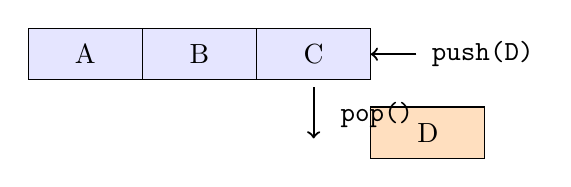
\begin{tikzpicture}[x=1.45cm,y=1cm]
        \foreach \i/\name in {0/A,1/B,2/C} {
            \draw[fill=blue!10] (\i,0) rectangle +(1,0.65);
            \node at (\i+0.5,0.32) {\name};
        }
        \draw[->,thick] (3.4,0.32) -- (3.0,0.32);
        \node[right] at (3.45,0.32) {\texttt{push(D)}};
        \draw[fill=orange!25] (3,-1.0) rectangle +(1,0.65);
        \node at (3.5,-0.68) {D};
        \draw[->,thick] (2.5,-0.1) -- (2.5,-0.75);
        \node[right] at (2.65,-0.45) {\texttt{pop()}};
    \end{tikzpicture}
    \caption{\texttt{push}と\texttt{pop}は配列の末尾を操作する}
    \label{fig:chapter18-iteration-push-pop}
\end{figure}

\begin{listing}[htbp]
\inputminted{ts}{listings/chapter18-iteration/push-pop-stack.ts}
\caption{\texttt{push}と\texttt{pop}で操作履歴を扱う}
\label{lst:chapter18-iteration-push-pop-stack}
\end{listing}

\texttt{push}は追加後の長さを返しますが、このサンプルでは戻り値を使わず、追加したという操作だけに注目しています。\texttt{pop}の戻り値は、取り出した要素です。ただし、配列が空のときに\texttt{pop}すると、値が取り出せないため\texttt{undefined}になります。この章では、初学者が安全に読めるように、\texttt{commands.length > 0}で空ではないことを確認してから\texttt{pop}しています。

\begin{pointbox}{スタックという考え方}
最後に入れたものを最初に取り出す構造を、スタックと呼びます。ゲームでは、直前の操作を取り消す、画面の状態を戻す、履歴をたどる、といった場面で似た考え方を使います。
\end{pointbox}

\section{先頭を操作する\texttt{shift}と\texttt{unshift}}

\texttt{shift}と\texttt{unshift}も、配列そのものの中身を変えるメソッドです。\texttt{shift}は配列の先頭から要素を1つ取り出し、その要素を返します。\texttt{unshift}は配列の先頭に要素を追加し、追加したあとの配列の長さを返します。末尾ではなく先頭を動かすため、時間の順番を持つリストや待ち行列を表すときに使えます。

\begin{figure}[htbp]
    \centering
    \begin{tikzpicture}[x=1.45cm,y=1cm]
        \node[left] at (-0.25,0.32) {\texttt{shift()}};
        \draw[->,thick] (0.0,0.32) -- (-0.65,0.32);
        \foreach \i/\name in {0/old,1/mid,2/new} {
            \draw[fill=green!12] (\i,0) rectangle +(1,0.65);
            \node at (\i+0.5,0.32) {\small \name};
        }
        \draw[->,thick] (-0.65,-0.8) -- (0,-0.8);
        \node[left] at (-0.7,-0.8) {\texttt{unshift(first)}};
    \end{tikzpicture}
    \caption{\texttt{shift}と\texttt{unshift}は配列の先頭を操作する}
    \label{fig:chapter18-iteration-shift-unshift}
\end{figure}

\begin{listing}[htbp]
\inputminted{ts}{listings/chapter18-iteration/shift-unshift-queue.ts}
\caption{\texttt{shift}と\texttt{push}でメッセージを古い順に処理する}
\label{lst:chapter18-iteration-shift-unshift-queue}
\end{listing}

このサンプルでは、\texttt{messages.push(...)}で新しいメッセージを末尾に追加し、\texttt{messages.shift()}で古いメッセージから取り出しています。\texttt{shift}したときに配列が空なら、戻り値は\texttt{undefined}になります。先に入ったものから順番に処理する構造を、キューと呼びます。

\begin{notebox}{\texttt{shift}と\texttt{unshift}は先頭を動かす}
\texttt{push}と\texttt{pop}は末尾、\texttt{shift}と\texttt{unshift}は先頭を操作します。名前だけでは向きが分かりにくいため、最初は図\ref{fig:chapter18-iteration-push-pop}と図\ref{fig:chapter18-iteration-shift-unshift}を見ながら確認しましょう。
\end{notebox}

\section{p5.jsで増減するリストを使う}

最後に、p5.jsの作品らしいサンプルとして、クリックした場所に小さな光を追加し、古い光から消していくプログラムを作ります。クリックするたびに配列へ追加し、数が多くなったら先頭から削除します。

\begin{listing}[htbp]
\inputminted[firstline=1,lastline=35]{ts}{listings/chapter18-iteration/click-sparkles.ts}
\caption{クリックで追加される光のクラス}
\label{lst:chapter18-iteration-sparkle-class}
\end{listing}

\begin{listing}[htbp]
\inputminted[firstline=37,lastline=73]{ts}{listings/chapter18-iteration/click-sparkles.ts}
\caption{\texttt{push}と\texttt{shift}で光のリストを管理する}
\label{lst:chapter18-iteration-sparkle-sketch}
\end{listing}

\texttt{sparkles.push(new Sparkle(...))}は、新しい光を末尾に追加します。\texttt{sparkles.length > maxSparkleCount}になったら、\texttt{sparkles.shift()}で古い光を先頭から削除します。こうすると、画面上に残る光の数を一定以下にできます。

\texttt{for...of}は、画面にあるすべての光を更新・描画するために使っています。光の番号は必要なく、光そのものを順番に使いたいので、\texttt{for...of}が読みやすい場面です。

\section{\texttt{for...in}で番号や名前を読む}

\texttt{for...in}は、配列やオブジェクトの「キー」を順番に取り出します。ここまでに扱った\texttt{for...of}は値を順番に取り出す構文でした。それに対して、\texttt{for...in}は値そのものではなく、値を取り出すための番号や名前を取り出します。少し考え方が違うため、この章では最後に紹介します。

\begin{listing}[htbp]
\inputminted{ts}{listings/chapter18-iteration/for-in-array.ts}
\caption{\texttt{for...in}で配列の番号を取り出す}
\label{lst:chapter18-iteration-for-in-array}
\end{listing}

\texttt{for...in}で取り出した\texttt{indexText}は文字列です。数値として使いたいときは、\texttt{Number(indexText)}で数値に変換します。この変換が必要になるため、配列の中身を読むだけなら\texttt{for...of}の方が書きやすいことが多いです。

\begin{listing}[htbp]
\inputminted{ts}{listings/chapter18-iteration/for-in-object.ts}
\caption{\texttt{for...in}で得点表の名前を取り出す}
\label{lst:chapter18-iteration-for-in-object}
\end{listing}

このサンプルでは、プレイヤー名をキー、得点を値として持つオブジェクトを使っています。\texttt{for...in}は、\texttt{"Aoi"}、\texttt{"Ren"}、\texttt{"Mika"}のようなキーを順番に取り出します。そのキーを使って\texttt{scores[playerName]}と書くと、対応する得点を取り出せます。

\begin{pointbox}{配列なら\texttt{for...of}、キーが欲しいなら\texttt{for...in}}
配列の値を順番に使いたいときは、まず\texttt{for...of}を考えます。配列の番号や、オブジェクトのプロパティ名が必要なときは、\texttt{for...in}を使う候補になります。
\end{pointbox}

\section{よくある間違い}

配列を増減させる処理では、何をどちら側から入れ、何をどちら側から取り出すのかが分からなくなりやすいです。名前と図を結びつけて、落ち着いて確認しましょう。

\begin{mistakebox}{\texttt{for...in}で値が取り出せると思ってしまう}
\texttt{for...in}で配列を読むと、取り出されるのは値そのものではなく番号です。値を読みたい場合は、基本的には\texttt{for...of}を使います。
\end{mistakebox}

\begin{mistakebox}{空の配列から\texttt{pop}や\texttt{shift}をしてしまう}
空の配列から値を取り出そうとすると、期待した値は得られません。取り出す前に\texttt{array.length > 0}を確認すると安全です。
\end{mistakebox}

\begin{mistakebox}{追加と削除の向きを混同する}
\texttt{push}と\texttt{pop}は末尾を操作します。\texttt{shift}と\texttt{unshift}は先頭を操作します。スタックなら\texttt{push}と\texttt{pop}、キューなら\texttt{push}と\texttt{shift}の組み合わせがよく使われます。
\end{mistakebox}

\begin{mistakebox}{\texttt{draw}の中で毎フレーム追加してしまう}
\texttt{draw}は何度も実行されます。\texttt{draw}の中で毎回\texttt{push}すると、配列がどんどん大きくなります。クリックやキー入力など、必要なタイミングだけで追加するようにします。
\end{mistakebox}

\section{まとめ}

この章では、配列を順番に読む\texttt{for...of}、キーを読む\texttt{for...in}、配列の末尾や先頭を操作する\texttt{push}、\texttt{pop}、\texttt{shift}、\texttt{unshift}を学びました。これらを使うと、数が変化するアイテム、効果、ログ、操作履歴などを扱いやすくなります。

次の章では、Life Gameを題材にして、同じ結果を得るための処理の進め方を工夫します。この章で学んだ「リストに記録する」考え方は、変化した場所を保存する処理にもつながります。

\section{演習問題}

この章の演習では、配列を読むだけでなく、実行中に増やしたり減らしたりする練習をします。どの操作が先頭を使い、どの操作が末尾を使うのかを意識しながら進めてください。

\begin{enumerate}
    \item \texttt{for...of}を使って、文字列の配列に入った名前をすべて表示してください。
    \item 数値の配列を作り、\texttt{for...of}を使って合計を求めてください。
    \item 文字列の配列に\texttt{push}で新しい値を追加し、追加前後の\texttt{length}を表示してください。
    \item \texttt{pop}を使って、最後に追加した値を取り出してください。
    \item \texttt{push}と\texttt{shift}を使って、古いメッセージから順に取り出すプログラムを作ってください。
    \item \texttt{unshift}を使って、重要なメッセージをリストの先頭に追加してください。
    \item クリックした位置を配列に保存し、\texttt{for...of}で全部の点を描くプログラムを作ってください。
    \item 点の数が20個を超えたら、\texttt{shift}で古い点を消すようにしてください。
    \item \texttt{for...in}を使って、配列の番号と値を両方表示してください。
    \item 挑戦問題として、最近押したキーを5個だけ表示するプログラムを作ってください。新しいキーを\texttt{push}し、6個以上になったら\texttt{shift}で古いキーを消します。
\end{enumerate}

\chapter{アルゴリズムを工夫する}
\label{chap:algorithm-improvement}

この章では、同じ結果を得るプログラムでも、処理の進め方を工夫すると速くできることを学びます。題材として、セルが生まれたり消えたりするLife Gameを使います。Life Gameは見た目には単純ですが、盤面が大きくなると「どのセルを調べるか」がとても大切になります。

\section{この章の概要}

これまでの章では、配列、クラス、ゲーム、画像、音声などを扱ってきました。この章では、それらを支える考え方として、アルゴリズムに注目します。アルゴリズムとは、問題を解くための手順のことです。

この章で扱う主な内容は次の通りです。

\begin{itemize}
    \item Life Gameの基本ルールを理解する
    \item 2次元配列でセルの状態を表す
    \item すべてのセルを調べて次の世代を作る
    \item 変化したセルを記録する
    \item 変化したセルの周囲だけを調べる
    \item 調べたセル数を表示して、処理の違いを見る
\end{itemize}

\begin{pointbox}{この章で見てほしいこと}
速いプログラムは、必ずしも短いプログラムではありません。何を調べ、何を調べなくてよいかを考えることで、同じ結果をより少ない処理で求められる場合があります。
\end{pointbox}

\section{Life Gameとは}

Life Gameは、格子状に並んだセルが、一定のルールにしたがって生き残ったり、死んだり、生まれたりするシミュレーションです。1つ1つのセルは、生きている状態と死んでいる状態のどちらかを持ちます。

次の世代の状態は、そのセルの周囲8マスにある生きているセルの数で決まります。

\begin{itemize}
    \item 生きているセルの周囲に生きているセルが2個または3個あると、生き残る
    \item 死んでいるセルの周囲に生きているセルが3個あると、新しく生まれる
    \item それ以外の場合、そのセルは死んだ状態になる
\end{itemize}

\begin{figure}[htbp]
    \centering
    \begin{tikzpicture}[scale=0.9]
        \foreach \x in {0,1,2} {
            \foreach \y in {0,1,2} {
                \draw[gray] (\x,\y) rectangle +(1,1);
            }
        }
        \fill[black!75] (1,1) rectangle +(1,1);
        \node at (1.5,1.5) {\textcolor{white}{中心}};
        \foreach \x/\y in {0/0,1/0,2/0,0/1,2/1,0/2,1/2,2/2} {
            \node at (\x+0.5,\y+0.5) {\small 周囲};
        }
    \end{tikzpicture}
    \caption{Life Gameで調べる周囲8マス}
    \label{fig:chapter18-neighbors}
\end{figure}

\section{2次元配列で盤面を表す}

Life Gameの盤面は、第13章で学んだ2次元配列で表せます。この章では、セルが生きているかどうかを\texttt{boolean}で表します。\texttt{true}なら生きているセル、\texttt{false}なら死んでいるセルです。

\begin{listing}[htbp]
\inputminted[firstline=1,lastline=38]{ts}{listings/chapter18/basic-life-game.ts}
\caption{Life Gameの盤面を2次元配列で作る}
\label{lst:chapter18-basic-board}
\end{listing}

\texttt{boolean[][]}は、\texttt{boolean}の配列をさらに配列にした型です。外側の配列を行、内側の配列を列として使うと、格子状のデータを表せます。現在の世代と次の世代の盤面を\texttt{boolean[][]}で表すと、生きているセルが\texttt{true}、死んでいるセルが\texttt{false}であることを型から読み取りやすくなります。

\begin{notebox}{行と列の順番}
この章のサンプルでは、\texttt{board[y][x]}の順でセルを取り出します。画面の座標が\texttt{x}、\texttt{y}の順なので少し迷いやすいですが、2次元配列では「何行目か」を先に指定すると考えると整理しやすくなります。
\end{notebox}

\section{単純な方法で次の世代を作る}

最初は、すべてのセルを順番に調べる方法で次の世代を作ります。この方法は素直で分かりやすく、Life Gameのルールを確認するには最適です。

\begin{listing}[htbp]
\inputminted{ts}{listings/chapter18/life-game-rules.ts}
\caption{周囲の生きているセルを数え、次の状態を決める}
\label{lst:chapter18-life-rules}
\end{listing}

\texttt{countLivingNeighbors}は、指定したセルの周囲8マスを調べます。盤面の外側にはセルがないため、\texttt{neighborX}や\texttt{neighborY}が範囲内かどうかを確認しています。

\texttt{getNextCellState}は、Life Gameのルールをそのまま関数にしたものです。今のセルが生きている場合と死んでいる場合で、次の状態の決まり方が少し変わります。

\begin{listing}[htbp]
\inputminted[firstline=1,lastline=35]{ts}{listings/chapter18/life-game-full-scan.ts}
\caption{全探索版のスケッチ}
\label{lst:chapter18-full-scan-sketch}
\end{listing}

\begin{listing}[htbp]
\inputminted[firstline=38,lastline=61]{ts}{listings/chapter18/life-game-full-scan.ts}
\caption{すべてのセルを調べて次の世代を作る}
\label{lst:chapter18-full-scan-update}
\end{listing}

\begin{listing}[htbp]
\inputminted[firstline=63,lastline=111]{ts}{listings/chapter18/life-game-full-scan.ts}
\caption{全探索版で使う近傍判定}
\label{lst:chapter18-full-scan-rules}
\end{listing}

この方法では、盤面の幅が60、高さが40なら、1世代進めるたびに2400個のセルを調べます。盤面が大きくなるほど、調べるセルの数は急に増えていきます。

\section{全探索版の弱点}

すべてのセルを調べる方法は、正しく動き、理解もしやすい方法です。ただし、盤面のほとんどが変化しない場合でも、毎回すべてのセルを調べます。

Life Gameでは、あるセルの次の状態は、そのセル自身と周囲8マスの状態だけで決まります。つまり、前の世代で遠く離れた場所だけが変化した場合、その影響はこのセルには届きません。この性質を使うと、次に調べる候補を減らせます。

\begin{pointbox}{変化の近くを見る}
あるセルが変化したとき、次の世代で影響を受ける可能性があるのは、そのセル自身と周囲8マスです。変化した場所から遠いセルは、前の世代と同じ近傍を見ているため、次の状態も変わりません。
\end{pointbox}

\begin{figure}[H]
    \centering
    \begin{tikzpicture}[font=\small]
        \node[font=\bfseries] at (1.65,0.7) {全探索};
        \foreach \row in {0,1,2,3,4} {
            \foreach \column in {0,1,2,3,4,5} {
                \fill[blue!13] (\column*0.55,-\row*0.55)
                    rectangle +(0.55,-0.55);
                \draw[gray] (\column*0.55,-\row*0.55)
                    rectangle +(0.55,-0.55);
            }
        }
        \fill[black!75] (2*0.55,-2*0.55)
            rectangle +(0.55,-0.55);
        \node[align=center] at (1.65,-3.35)
            {盤面の全30マスを調べる\\
             （実際のサンプルでは60×40マス）};

        \begin{scope}[xshift=7.3cm]
            \node[font=\bfseries] at (1.65,0.7) {変化した周囲だけを調べる};
            \foreach \row in {0,1,2,3,4} {
                \foreach \column in {0,1,2,3,4,5} {
                    \fill[gray!5] (\column*0.55,-\row*0.55)
                        rectangle +(0.55,-0.55);
                    \draw[gray] (\column*0.55,-\row*0.55)
                        rectangle +(0.55,-0.55);
                }
            }
            \foreach \row in {1,2,3} {
                \foreach \column in {1,2,3} {
                    \fill[green!18] (\column*0.55,-\row*0.55)
                        rectangle +(0.55,-0.55);
                    \draw[green!45!black] (\column*0.55,-\row*0.55)
                        rectangle +(0.55,-0.55);
                }
            }
            \fill[orange!80] (2*0.55,-2*0.55)
                rectangle +(0.55,-0.55);
            \node[white, font=\bfseries] at (2*0.55+0.275,-2*0.55-0.275)
                {変};
            \node[align=center] at (1.65,-3.35)
                {変化したセルと周囲8マスだけを候補にする\\
                 この例では9マス};
        \end{scope}
    \end{tikzpicture}
    \caption{全探索と変化した周囲だけを調べる方法の違い}
    \label{fig:chapter19-full-scan-and-candidates}
\end{figure}

図\ref{fig:chapter19-full-scan-and-candidates}の右側では、オレンジ色のセルが前の世代で変化した場所です。次の世代では、そのセルと緑色で示した周囲だけを候補にします。盤面の変化が一部に限られていれば、左側の全探索よりも調べるセルを大きく減らせます。

\section{変化した場所をリストに保存する}

次に、変化した場所をリストとして保存します。ここでは\texttt{CellPosition}という小さなクラスを作り、セルの\texttt{x}座標と\texttt{y}座標をまとめて扱います。

\begin{listing}[htbp]
\inputminted[firstline=1,lastline=46]{ts}{listings/chapter18/life-game-changed-cells.ts}
\caption{変化したセルの位置を記録する}
\label{lst:chapter18-changed-cells-position}
\end{listing}

\begin{listing}[htbp]
\inputminted[firstline=60,lastline=103]{ts}{listings/chapter18/life-game-changed-cells.ts}
\caption{変化したセルとその周囲を候補に入れる}
\label{lst:chapter18-changed-cells-candidates}
\end{listing}

\texttt{changedCells}には、前の世代から状態が変わったセルの位置を入れます。次の世代を作るときは、そのセル自身と周囲8マスを候補として調べます。

\texttt{addPositionIfNeeded}は、同じ位置を何度もリストに入れないための関数です。ここでは、初学者が追いやすいように、配列を順番に見て同じ座標があるかどうかを調べています。

\section{変化した周囲だけで次の世代を作る}

変化した場所のリストを使うと、すべてのセルを調べなくても次の世代を作れます。ただし、注意点があります。新しい世代の盤面を作るとき、調べなかったセルは前の世代と同じ状態として残す必要があります。

\begin{listing}[htbp]
\inputminted[firstline=1,lastline=36]{ts}{listings/chapter18/life-game-optimized.ts}
\caption{差分更新版で使う位置と結果のクラス}
\label{lst:chapter18-optimized-classes}
\end{listing}

\begin{listing}[htbp]
\inputminted[firstline=38,lastline=83]{ts}{listings/chapter18/life-game-optimized.ts}
\caption{差分更新版で使う候補リストの補助関数}
\label{lst:chapter18-optimized-candidates}
\end{listing}

\begin{listing}[htbp]
\inputminted[firstline=85,lastline=119]{ts}{listings/chapter18/life-game-optimized.ts}
\caption{変化した周囲だけを調べて次の世代を作る}
\label{lst:chapter18-optimized-update}
\end{listing}

\begin{listing}[htbp]
\inputminted[firstline=121,lastline=141]{ts}{listings/chapter18/life-game-optimized.ts}
\caption{変化したセルの周囲を候補に加える}
\label{lst:chapter18-optimized-around-cells}
\end{listing}

\begin{listing}[htbp]
\inputminted[firstline=251,lastline=289]{ts}{listings/chapter18/life-game-optimized.ts}
\caption{差分更新版のLife Gameを動かす}
\label{lst:chapter18-optimized-sketch}
\end{listing}

\texttt{copyBoard}で現在の盤面をコピーしてから、候補になったセルだけを更新しています。これにより、調べなかったセルはそのまま残ります。

この方法は、変化する場所が少ないときに効果を発揮します。一方で、盤面全体が激しく変化している場合は、候補が多くなり、全探索版との差が小さくなります。

\section{調べたセル数を比べる}

アルゴリズムの違いは、見た目だけでは分かりにくいことがあります。そこで、1世代を作るために調べたセル数を画面に表示します。

\begin{listing}[htbp]
\inputminted[firstline=1,lastline=36]{ts}{listings/chapter18/life-game-comparison.ts}
\caption{比較用サンプルで使う位置と結果のクラス}
\label{lst:chapter18-comparison-classes}
\end{listing}

\begin{listing}[htbp]
\inputminted[firstline=38,lastline=59]{ts}{listings/chapter18/life-game-comparison.ts}
\caption{比較用サンプルの全探索版}
\label{lst:chapter18-comparison-full-scan}
\end{listing}

\begin{listing}[htbp]
\inputminted[firstline=61,lastline=95]{ts}{listings/chapter18/life-game-comparison.ts}
\caption{比較用サンプルの差分更新版}
\label{lst:chapter18-comparison-changed-cells}
\end{listing}

\begin{listing}[htbp]
\inputminted[firstline=261,lastline=293]{ts}{listings/chapter18/life-game-comparison.ts}
\caption{比較用サンプルの準備}
\label{lst:chapter18-comparison-setup}
\end{listing}

\begin{listing}[htbp]
\inputminted[firstline=315,lastline=327]{ts}{listings/chapter18/life-game-comparison.ts}
\caption{比較結果を画面に表示して世代を進める}
\label{lst:chapter18-comparison-sketch}
\end{listing}

このサンプルでは、同じ盤面に対して、全探索版なら何個のセルを調べるか、差分更新版なら何個の候補を調べるかを表示します。最初のうちは差が小さくても、動きが落ち着いてくると、差分更新版の調べる数が少なくなることがあります。

\begin{figure}[htbp]
    \centering
    \begin{tikzpicture}[x=1.15cm, y=0.85cm, font=\small]
        \draw[->, thick] (0,0) -- (8.6,0)
            node[right]{世代};
        \draw[->, thick] (0,0) -- (0,5.3)
            node[above, align=center]{調べた\\セル数};

        \draw[blue!70!black, very thick]
            (0.4,4.45) -- (8.0,4.45);
        \node[blue!70!black, anchor=west] at (5.0,4.78)
            {全探索：盤面全体なので一定};
        \node[blue!70!black, anchor=east] at (8.0,4.15)
            {2400セル（60×40）};

        \draw[orange!85!black, very thick]
            plot[smooth] coordinates {
                (0.4,3.9) (1.6,3.55) (2.8,2.85)
                (4.0,2.05) (5.2,1.45) (6.4,1.15) (7.8,1.35)
            };
        \foreach \x/\y in {
            0.4/3.9,1.6/3.55,2.8/2.85,4.0/2.05,
            5.2/1.45,6.4/1.15,7.8/1.35
        } {
            \fill[orange!85!black] (\x,\y) circle (1.8pt);
        }
        \node[orange!85!black, anchor=west, align=left]
            at (4.3,2.65)
            {差分更新：変化が減ると\\候補も少なくなる};
    \end{tikzpicture}
    \caption{変化が少なくなる場合に調べるセル数が変わる概念図}
    \label{fig:chapter19-checked-cell-counts}
\end{figure}

図\ref{fig:chapter19-checked-cell-counts}は、変化が次第に少なくなる場合の傾向を表した概念図です。差分更新版の線は実測値ではなく、実際に調べるセル数は初期状態や世代ごとの変化によって異なります。全探索版は、変化の量にかかわらず毎回2400セルを調べます。

\begin{notebox}{速さの比較は条件によって変わる}
差分更新版はいつでも必ず速いわけではありません。候補を作る処理や、重複を取り除く処理にも時間がかかります。大切なのは、「どのようなデータのときに有利か」を考えることです。
\end{notebox}

\section{よくある間違い}

Life Gameは、ルールは短いものの、配列のコピーや座標の扱いで間違えやすい題材です。思った通りに動かないときは、次の点を確認します。

\begin{mistakebox}{現在の盤面を直接書き換えてしまう}
次の世代を作る途中で現在の盤面を書き換えると、まだ調べていないセルの判定に影響してしまいます。現在の盤面を読みながら、別の配列に次の世代を書き込むようにします。
\end{mistakebox}

\begin{mistakebox}{盤面の外側を読もうとしてしまう}
端のセルでは、周囲8マスの一部が盤面の外になります。\texttt{x}や\texttt{y}が範囲内かどうかを確認してから配列を読む必要があります。
\end{mistakebox}

\begin{mistakebox}{同じ候補を何度も追加してしまう}
変化したセルが近くにあると、同じ候補が何度も出てきます。同じセルを何度も調べると、差分更新の効果が小さくなります。
\end{mistakebox}

\begin{mistakebox}{最初から難しい高速化を目指してしまう}
まずは全探索版を正しく作ることが大切です。正しい結果が分かってから、同じ結果になるように差分更新版へ変えていきます。
\end{mistakebox}

\section{まとめ}

この章では、Life Gameを題材にして、アルゴリズムを工夫する考え方を学びました。最初にすべてのセルを調べる分かりやすい方法を作り、その後、変化した場所を記録して調べる候補を減らす方法へ進みました。

重要なのは、速くする前に正しく動く方法を作ることです。そのうえで、どこに無駄があるのか、どの情報を保存しておくと次の処理で役立つのかを考えると、プログラムを改善しやすくなります。

\section{演習問題}

この章の演習では、Life Gameのルールを確認しながら、少しずつアルゴリズムの工夫に挑戦します。

\begin{enumerate}
    \item Life Gameで、死んでいるセルが次の世代で生まれる条件を説明しなさい。
    \item \texttt{board[y][x]}の\texttt{x}と\texttt{y}が何を表しているか説明しなさい。
    \item セルの大きさを変えて、同じ盤面を大きく表示しなさい。
    \item 初期状態で生きているセルの割合を変え、動きがどう変わるか観察しなさい。
    \item 生きているセルの色と死んでいるセルの色を変更しなさい。
    \item 全探索版で、1世代ごとに調べたセル数を画面に表示しなさい。
    \item 変化したセルの位置を画面上で別の色で表示しなさい。
    \item 差分更新版と全探索版が同じ結果になるか、同じ初期状態で比べなさい。
    \item マウスでクリックした場所のセルを生きている状態に変えられるようにしなさい。
    \item Life Gameの有名な形を調べ、グライダーなどの初期状態を作りなさい。
    \item 調べたセル数の変化を折れ線グラフのように表示する方法を考えなさい。
\end{enumerate}

\chapter{落ち葉拾いで学ぶポリモーフィズム}
\label{chap:polymorphism-leaf-collector}

この章では、第11章で学んだクラスと、第14章で学んだ継承をもう一歩進めて、ポリモーフィズムと\texttt{interface}について学びます。題材は、画面上に落ちてくる落ち葉をプレイヤーが拾う小さなゲームです。

ポリモーフィズムは難しい言葉ですが、ここでは「同じ呼び方で、違う種類のものを動かすこと」と考えます。落ち葉、金色の落ち葉、石のように見た目や点数が違うものでも、\texttt{update}、\texttt{display}、\texttt{isCollected}を持つなら、同じ配列に入れて同じ手順で扱えます。

\section{この章の概要}

この章は、興味を持った学生向けの発展的な話題です。すべてを一度で理解しようとするよりも、「同じ呼び方で扱えるように設計すると、ゲームを広げやすくなる」という感覚をつかむことを目標にします。

この章で扱う主な内容は次の通りです。

\begin{itemize}
    \item クラスを使って落ち葉を1つの部品として表す
    \item \texttt{interface}で「必要なメソッドの約束」を書く
    \item \texttt{implements}で約束を満たすクラスを作る
    \item \texttt{CollectibleItem[]}で違う種類のものを同じ配列に入れる
    \item ポリモーフィズムにより、同じ呼び方で違う動きを実行する
    \item 継承と\texttt{interface}の使い分けを考える
\end{itemize}

\begin{notebox}{この章は少し背伸びした内容}
\texttt{interface}やポリモーフィズムは、プログラムが少し大きくなってから便利さが見えやすい考え方です。最初は書き方を暗記するより、「同じ使い方ができるものをまとめる約束」として読むところから始めましょう。
\end{notebox}

\section{まずは1枚の落ち葉を動かす}

最初に、クラスを使わずに1枚の落ち葉を動かします。落ち葉は下へ落ちながら、左右に少し揺れるようにします。

\begin{listing}[htbp]
\inputminted[firstline=1,lastline=26]{ts}{listings/chapter19/single-leaf.ts}
\caption{1枚の落ち葉を動かすスケッチ}
\label{lst:chapter19-single-leaf-sketch}
\end{listing}

\begin{listing}[htbp]
\inputminted[firstline=28,lastline=36]{ts}{listings/chapter19/single-leaf.ts}
\caption{落ち葉の位置を更新する関数}
\label{lst:chapter19-single-leaf-update}
\end{listing}

\begin{listing}[htbp]
\inputminted[firstline=38,lastline=55]{ts}{listings/chapter19/single-leaf.ts}
\caption{落ち葉を揺らしながら描く関数}
\label{lst:chapter19-single-leaf-display}
\end{listing}

このサンプルでは、\texttt{leafX}、\texttt{leafY}、\texttt{leafSpeedY}などの変数で落ち葉の状態を表しています。1枚だけなら十分に読めますが、落ち葉が10枚、20枚と増えると、変数を増やすだけでは管理しにくくなります。

\begin{pointbox}{同じ種類のものが増える合図}
落ち葉を何枚も出したくなったら、\texttt{leafX1}、\texttt{leafX2}のように変数名を増やすより、クラスや配列でまとめることを考えます。
\end{pointbox}

\section{落ち葉をクラスにする}

次に、落ち葉を\texttt{FallingLeaf}クラスとして表します。位置、速さ、色、揺れ方をフィールドにし、動かす処理を\texttt{update}、描く処理を\texttt{display}にまとめます。

\begin{listing}[htbp]
\inputminted[firstline=1,lastline=30]{ts}{listings/chapter19/leaf-class.ts}
\caption{\texttt{FallingLeaf}クラスのフィールドとコンストラクタ}
\label{lst:chapter19-leaf-class-constructor}
\end{listing}

\begin{listing}[htbp]
\inputminted[firstline=32,lastline=57]{ts}{listings/chapter19/leaf-class.ts}
\caption{\texttt{FallingLeaf}の更新と描画}
\label{lst:chapter19-leaf-class-methods}
\end{listing}

\begin{listing}[htbp]
\inputminted[firstline=60,lastline=73]{ts}{listings/chapter19/leaf-class.ts}
\caption{\texttt{FallingLeaf}を使うスケッチ}
\label{lst:chapter19-leaf-class-sketch}
\end{listing}

第11章で学んだように、クラスは同じ形のインスタンスを作るための設計図です。落ち葉が複数になっても、\texttt{new FallingLeaf(...)}でインスタンスを増やせます。

ただし、この章で作りたいゲームでは、拾えるものが落ち葉だけとは限りません。得点の高い金色の落ち葉や、拾うと減点される石も出したくなるかもしれません。そのとき、すべてを\texttt{FallingLeaf}の子クラスにするべきでしょうか。

\section{\texttt{interface}は使い方の約束}

\texttt{interface}は、クラスがどのようなメソッドを持つべきかを表す約束です。ここでは、拾えるものを\texttt{CollectibleItem}という\texttt{interface}で表します。

\begin{listing}[htbp]
\inputminted[firstline=1,lastline=8]{ts}{listings/chapter19/collectible-interface.ts}
\caption{拾えるものに必要なメソッドを表す\texttt{interface}}
\label{lst:chapter19-collectible-interface}
\end{listing}

\texttt{CollectibleItem}は、\texttt{update}、\texttt{display}、\texttt{isCollected}、\texttt{isOutsideCanvas}、\texttt{getScore}を持つことを約束しています。これは「拾えるものなら、少なくともこの5つの呼び方ができる」という意味です。

\begin{center}
\begin{tabular}{ll}
\toprule
メソッド & 役割 \\
\midrule
\texttt{update(p)} & アイテムの状態を変える \\
\texttt{display(p)} & アイテムを画面に描く \\
\texttt{isCollected(player)} & プレイヤーが拾ったか判定する \\
\texttt{isOutsideCanvas(p)} & 画面外に出たか判定する \\
\texttt{getScore()} & 拾ったときの点数を返す \\
\bottomrule
\end{tabular}
\end{center}

\begin{pointbox}{\texttt{interface}は中身を書かない}
\texttt{interface}には、メソッドの名前、引数、戻り値の型を書きます。実際にどのように動くかは、それを\texttt{implements}するクラス側に書きます。
\end{pointbox}

\section{\texttt{implements}で約束を満たす}

クラスが\texttt{interface}の約束を満たすことを、\texttt{implements}で表します。次の例では、\texttt{ScoreLeaf}が\texttt{CollectibleItem}を実装しています。

\begin{listing}[htbp]
\inputminted[firstline=10,lastline=35]{ts}{listings/chapter19/collectible-interface.ts}
\caption{プレイヤーを表す\texttt{Player}クラス}
\label{lst:chapter19-player-class}
\end{listing}

\begin{listing}[htbp]
\inputminted[firstline=37,lastline=80]{ts}{listings/chapter19/collectible-interface.ts}
\caption{\texttt{CollectibleItem}を実装する落ち葉}
\label{lst:chapter19-score-leaf}
\end{listing}

\texttt{ScoreLeaf implements CollectibleItem}と書くと、\texttt{ScoreLeaf}は\texttt{CollectibleItem}で約束したメソッドをすべて持つ必要があります。もし\texttt{getScore}を書き忘れると、TypeScriptが教えてくれます。

\begin{notebox}{型は設計ミスに早く気づくためにも役立つ}
\texttt{interface}を使うと、「拾えるもの」として必要なメソッドの書き忘れに気づきやすくなります。ゲームの要素が増えるほど、この助けは大きくなります。
\end{notebox}

\section{判定処理を読みやすくする}

距離の計算は、クラスごとに何度も書くと読みにくくなります。ここでは、プレイヤーとアイテムが近いかどうかを調べる\texttt{isNear}関数を用意します。

\begin{listing}[htbp]
\inputminted[firstline=1,lastline=23]{ts}{listings/chapter19/interface-without-vector.ts}
\caption{距離判定を関数に分ける}
\label{lst:chapter19-interface-helper}
\end{listing}

\begin{listing}[htbp]
\inputminted[firstline=25,lastline=61]{ts}{listings/chapter19/interface-without-vector.ts}
\caption{距離判定の関数を使う落ち葉}
\label{lst:chapter19-interface-leaf-with-helper}
\end{listing}

\texttt{isNear}は、アイテムの座標、プレイヤー、判定距離を受け取り、近ければ\texttt{true}を返します。このように、複数のクラスで使う処理は関数に分けておくと、同じ計算をあちこちに書かずにすみます。

\section{ポリモーフィズムで同じ配列に入れる}

ポリモーフィズムは、同じ型として扱っているものが、実際にはそれぞれ違う動きをすることです。次のサンプルでは、普通の落ち葉と金色の落ち葉をどちらも\texttt{CollectibleItem}として扱います。

\begin{listing}[htbp]
\inputminted[firstline=1,lastline=49]{ts}{listings/chapter19/polymorphism-items.ts}
\caption{ポリモーフィズムで使う共通部分}
\label{lst:chapter19-polymorphism-base}
\end{listing}

\begin{listing}[htbp]
\inputminted[firstline=51,lastline=87]{ts}{listings/chapter19/polymorphism-items.ts}
\caption{普通の落ち葉を表す\texttt{LeafItem}}
\label{lst:chapter19-polymorphism-leaf}
\end{listing}

\begin{listing}[htbp]
\inputminted[firstline=89,lastline=127]{ts}{listings/chapter19/polymorphism-items.ts}
\caption{得点の高い\texttt{GoldenLeafItem}}
\label{lst:chapter19-polymorphism-golden-leaf}
\end{listing}

\begin{listing}[htbp]
\inputminted[firstline=4,lastline=49]{ts}{listings/chapter19/polymorphism-sketch.ts}
\caption{\texttt{CollectibleItem[]}でまとめて動かす}
\label{lst:chapter19-polymorphism-sketch}
\end{listing}

\texttt{items}は\texttt{CollectibleItem[]}型です。この配列には、\texttt{LeafItem}も\texttt{GoldenLeafItem}も入れられます。どちらも\texttt{CollectibleItem}の約束を満たしているからです。

\begin{pointbox}{同じ呼び方で違う結果になる}
\texttt{item.display(p)}と同じ呼び方をしても、普通の落ち葉なら茶色の葉、金色の落ち葉なら光る葉が描かれます。\texttt{item.getScore()}も、普通の落ち葉なら10点、金色の落ち葉なら30点を返します。
\end{pointbox}

\section{減点アイテムを追加する}

\texttt{interface}で設計しておくと、新しい種類のアイテムを追加しやすくなります。次の例では、拾うと点数が下がる石を追加します。

\begin{listing}[htbp]
\inputminted{ts}{listings/chapter19/harmful-item.ts}
\caption{減点される石とランダムなアイテム追加}
\label{lst:chapter19-harmful-item}
\end{listing}

\texttt{StoneItem}も\texttt{CollectibleItem}を実装しているため、\texttt{items}配列に入れられます。\texttt{getScore}が\texttt{-20}を返すので、拾ったときに得点が下がります。

\begin{figure}[htbp]
    \centering
    \begin{tikzpicture}[
        interfacebox/.style={
            rectangle,
            draw,
            rounded corners,
            align=center,
            minimum width=56mm,
            minimum height=14mm,
            fill=gray!10
        },
        classbox/.style={
            rectangle,
            draw,
            rounded corners,
            align=center,
            minimum width=36mm,
            minimum height=13mm
        },
        arraybox/.style={
            rectangle,
            draw,
            rounded corners,
            align=center,
            minimum width=92mm,
            minimum height=13mm,
            fill=gray!6
        },
        arrow/.style={->, thick},
        implementarrow/.style={->, thick, dashed}
    ]
        \node[interfacebox] (interface) at (0, 1.8) {
            \texttt{CollectibleItem}\\
            \footnotesize 共通の呼び方の約束
        };

        \node[classbox] (leaf) at (-4.4, -0.5) {
            \texttt{LeafItem}\\
            \footnotesize 普通の落ち葉\\
            \footnotesize \texttt{getScore()}は10
        };
        \node[classbox] (golden) at (0, -0.5) {
            \texttt{GoldenLeafItem}\\
            \footnotesize 金色の落ち葉\\
            \footnotesize \texttt{getScore()}は30
        };
        \node[classbox] (stone) at (4.4, -0.5) {
            \texttt{StoneItem}\\
            \footnotesize 石\\
            \footnotesize \texttt{getScore()}は-20
        };

        \node[arraybox] (array) at (0, -3.0) {
            \texttt{const items: CollectibleItem[] = [leaf, goldenLeaf, stone];}\\
            \footnotesize 同じ配列に入れて、同じメソッド名で扱える
        };

        \draw[implementarrow] (leaf) -- node[left, font=\footnotesize] {\texttt{implements}} (interface);
        \draw[implementarrow] (golden) -- node[right, font=\footnotesize] {\texttt{implements}} (interface);
        \draw[implementarrow] (stone) -- node[right, font=\footnotesize] {\texttt{implements}} (interface);

        \draw[arrow] (leaf) -- (array);
        \draw[arrow] (golden) -- (array);
        \draw[arrow] (stone) -- (array);
    \end{tikzpicture}
    \caption{\texttt{CollectibleItem}と複数のアイテムクラスの関係}
    \label{fig:chapter19-collectible-item-classes}
\end{figure}

図\ref{fig:chapter19-collectible-item-classes}のように、\texttt{LeafItem}、\texttt{GoldenLeafItem}、\texttt{StoneItem}は、それぞれ違う見た目や点数を持っています。それでも、どれも\texttt{CollectibleItem}の約束を満たしているため、\texttt{CollectibleItem[]}型の配列にまとめられます。

ここで大切なのは、メインの更新処理を大きく変えなくてよいことです。普通の落ち葉、金色の落ち葉、石のどれであっても、\texttt{update}、\texttt{display}、\texttt{isCollected}、\texttt{isOutsideCanvas}、\texttt{getScore}を同じように呼び出せます。

\section{継承と\texttt{interface}の違い}

第14章では、共通するフィールドやメソッドを親クラスにまとめる継承を学びました。一方、\texttt{interface}は「どのように呼び出せるか」を決める約束です。

\begin{center}
\begin{tabular}{lll}
\toprule
仕組み & 得意なこと & 考え方 \\
\midrule
継承 & 共通する実装をまとめる & \texttt{A}は\texttt{B}の一種 \\
\texttt{interface} & 同じ使い方を約束する & \texttt{A}はこの呼び方ができる \\
\bottomrule
\end{tabular}
\end{center}

たとえば、\texttt{LeafItem}と\texttt{GoldenLeafItem}は、共通部分が多いので親クラスを作る選択もできます。一方、石、鍵、回復アイテム、ゴール地点のように見た目も役割も違うものは、無理に親子関係にするより、\texttt{CollectibleItem}という使い方の約束でまとめる方が自然な場合があります。

\begin{notebox}{迷ったときの考え方}
共通するデータや処理をまとめたいなら継承、同じ配列に入れて同じメソッドを呼びたいなら\texttt{interface}を考えます。実際のプログラムでは、両方を組み合わせることもあります。
\end{notebox}

\section{小さなゲームへ広げる}

最後に、アイテムをランダムに追加する形へ近づけます。この例では、前のサンプルで定義した\texttt{Player}、\texttt{CollectibleItem}、\texttt{LeafItem}、\texttt{GoldenLeafItem}、\texttt{StoneItem}、\texttt{addRandomItem}を使う想定です。

\begin{listing}[htbp]
\inputminted{ts}{listings/chapter19/complete-leaf-game.ts}
\caption{落ち葉拾いゲームの全体の流れ}
\label{lst:chapter19-complete-leaf-game}
\end{listing}

このサンプルでは、アイテムを後ろから順番に見ています。途中で\texttt{items.splice(index, 1)}により配列からアイテムを取り除くため、前から順番に進むより、後ろから進む方が添え字のずれを避けやすくなります。

\begin{mistakebox}{消す処理と配列の順番}
配列の途中の要素を消すと、その後ろにあった要素の添え字が変わります。配列から要素を消しながら調べるときは、後ろから前へ進む方法がよく使われます。
\end{mistakebox}

\section{よくある間違い}

\texttt{interface}を使う章では、書き方そのものよりも、どこに何を書くかで迷いやすくなります。エラーが出たときは、約束したメソッドをすべて書いているか、戻り値の型が合っているかを確認します。

\begin{mistakebox}{\texttt{interface}に処理の中身を書こうとする}
\texttt{interface}には、メソッドの形だけを書きます。実際の処理は、\texttt{implements}するクラスの中に書きます。
\end{mistakebox}

\begin{mistakebox}{約束したメソッドを書き忘れる}
\texttt{CollectibleItem}に\texttt{getScore}があるなら、\texttt{implements CollectibleItem}するクラスには\texttt{getScore}が必要です。名前、引数、戻り値の型をそろえます。
\end{mistakebox}

\begin{mistakebox}{親クラスと\texttt{interface}を同じものだと思う}
親クラスはフィールドや処理の中身を持てます。\texttt{interface}は「この呼び方ができる」という約束です。役割が違うため、どちらを使うかは目的で決めます。
\end{mistakebox}

\begin{mistakebox}{共通の配列から個別のメソッドを呼ぼうとする}
\texttt{CollectibleItem[]}の要素から呼べるのは、\texttt{CollectibleItem}に書かれているメソッドです。特定のクラスだけが持つメソッドを呼びたい場合は、そのメソッドも\texttt{interface}に含めるべきか考えます。
\end{mistakebox}

\section{まとめ}

この章では、落ち葉拾いゲームを題材にして、\texttt{interface}とポリモーフィズムを学びました。\texttt{interface}は、クラスが持つべきメソッドの約束を表します。\texttt{implements}を使うと、その約束を満たすクラスを作れます。

ポリモーフィズムを使うと、普通の落ち葉、金色の落ち葉、石のように違う種類のものを、\texttt{CollectibleItem[]}としてまとめて扱えます。同じ\texttt{update}、\texttt{display}、\texttt{isCollected}、\texttt{isOutsideCanvas}、\texttt{getScore}を呼び出しても、実際に動く処理はインスタンスごとに変わります。

継承は共通する実装をまとめる方法で、\texttt{interface}は同じ使い方を約束する方法です。ゲームの要素が増えてきたとき、この2つを使い分けられると、プログラムを広げやすくなります。

\section{演習問題}

この章の演習では、まず\texttt{interface}の読み方を確認し、次に落ち葉拾いゲームへ新しいアイテムやルールを追加していきます。

\begin{enumerate}
    \item \texttt{CollectibleItem}に書かれている5つのメソッドの役割を説明しなさい。
    \item \texttt{LeafItem}の\texttt{getScore}が返す点数を変更しなさい。
    \item \texttt{GoldenLeafItem}の見た目を変更し、普通の落ち葉と区別しやすくしなさい。
    \item \texttt{StoneItem}の減点を\texttt{-20}から別の値に変更しなさい。
    \item \texttt{addRandomItem}で、金色の落ち葉が出る確率を上げなさい。
    \item 新しい\texttt{RedLeafItem}を作り、拾うと20点入るようにしなさい。
    \item 一定時間だけ得点が2倍になる\texttt{BonusItem}の設計を考えなさい。
    \item \texttt{isOutsideCanvas}の判定距離を変更し、画面外に出たアイテムが消えるタイミングを変えなさい。
    \item \texttt{LeafItem}と\texttt{GoldenLeafItem}に共通する処理を親クラスにまとめる案を考えなさい。
    \item \texttt{interface}を使う場合と継承を使う場合の違いを、自分の言葉で説明しなさい。
    \item 挑戦問題として、プレイヤーのHPを追加し、石を拾うとHPが減るゲームに発展させなさい。
\end{enumerate}

\chapter{総合演習：小さな作品を完成させる}
\label{chap:final-projects}

この章では、これまでに学んだ内容を使って、1つの作品を完成させます。ここでの目標は、すべての技術を使うことではありません。自分で課題を選び、完成までの道筋を考え、必要な機能を少しずつ作っていく経験をすることです。

総合演習では、学生ごとに取り組む課題が違っていてかまいません。得意な人は発展的な機能に挑戦し、まだ自信がない人は、まず確実に動く小さな作品を作ることを目指します。作品の大きさよりも、「自分で考えて、動く形にした」ことを大切にします。

\section{この章の概要}

この章は、通常の解説章ではなく、制作課題を選ぶためのガイドです。各課題は、1週間から2週間程度で取り組むことを想定しています。

この章で扱う内容は次の通りです。

\begin{itemize}
    \item 総合演習の進め方
    \item 課題を選ぶときの考え方
    \item 提出物の条件
    \item 評価の観点
    \item 難易度別の課題一覧
    \item 制作計画と振り返り
\end{itemize}

\begin{pointbox}{完成の大きさを自分で調整する}
総合演習では、同じ課題でも完成の形を変えられます。まず最低限の完成条件を満たし、時間があれば見た目、音、データ保存、難易度調整などを追加していきましょう。
\end{pointbox}

\section{総合演習の進め方}

総合演習では、課題一覧から1つを選びます。選んだ課題をそのまま作ってもよいですし、テーマや見た目を自分なりに変えてもかまいません。

制作は、次のような流れで進めます。

\begin{enumerate}
    \item 課題を1つ選ぶ
    \item 最低限の完成条件を確認する
    \item 画面に何を表示するかを紙やメモに描く
    \item 必要な変数、関数、クラスを考える
    \item まず小さく動くものを作る
    \item 少しずつ機能を追加する
    \item 動作確認をして、説明できる形に整える
\end{enumerate}

\begin{notebox}{最初から完成形を作ろうとしない}
最初からすべての機能を入れようとすると、どこで動かなくなったのか分かりにくくなります。まずは「丸が動く」「点数が増える」「画面が切り替わる」のような小さな成功を作りましょう。
\end{notebox}

\section{提出物の条件}

提出物は、作品そのものだけではなく、作品を説明するための情報も含めます。プログラムを見た人が、何を作ろうとしたのか、どこを工夫したのかを理解できるようにします。

提出物には、次の内容を含めます。

\begin{itemize}
    \item TypeScript + p5.jsで作成したプログラム
    \item 作品名
    \item 作品の説明
    \item 操作方法
    \item 工夫した点
    \item うまくいかなかった点や、今後追加したい点
\end{itemize}

プログラムは、授業で扱ってきたp5.jsのinstance modeを基本とします。変数名、関数名、クラス名は、あとから読んでも意味が分かる名前にします。

\section{評価の観点}

総合演習では、単に機能が多い作品だけを高く評価するのではありません。自分の理解に合わせて設計し、読みやすく動く形にしたことも重要です。

評価では、主に次の観点を見ます。

\begin{center}
\begin{tabular}{ll}
\toprule
観点 & 内容 \\
\midrule
動作 & 作品が実行でき、主要な機能が動く \\
読みやすさ & 変数名、関数名、クラス名が分かりやすい \\
構造 & 関数、配列、クラスなどを適切に使っている \\
工夫 & 見た目、動き、ルール、演出に自分なりの工夫がある \\
説明 & 作品の目的や操作方法を説明できる \\
振り返り & できたこと、難しかったこと、改善点を書ける \\
\bottomrule
\end{tabular}
\end{center}

\begin{pointbox}{難しい機能を使えばよいわけではない}
高度な機能を無理に入れるより、作品の目的に合った書き方を選ぶことが大切です。小さくても、よく整理されていて遊びやすい作品はよい作品です。
\end{pointbox}

\section{難易度の目安}

課題は、AからDまでの難易度に分けています。Aは基礎を確認しながら作る課題、Dは発展的な設計に挑戦する課題です。

\begin{center}
\begin{tabular}{lll}
\toprule
難易度 & 目安 & 主に使う内容 \\
\midrule
A & 基礎 & 図形、変数、条件分岐、マウス、キーボード \\
B & 標準 & 配列、関数、クラス、当たり判定、ゲームの状態 \\
C & 発展 & 画像、文字、音声、JSON、保存、アルゴリズム \\
D & 挑戦 & 継承、interface、設計の工夫、自由制作 \\
\bottomrule
\end{tabular}
\end{center}

自分にとって少し難しいと感じる課題を選ぶと、制作を通して学べることが増えます。ただし、難しすぎる課題を選ぶと、最後まで動く形にできないことがあります。迷ったときは、最低限の完成条件を見て選びましょう。

\section{A：基礎を固める課題}

このレベルの課題では、まず1つの画面で動く作品を作ることを目指します。図形、色、変数、条件分岐、マウスやキーボード操作を使って、確実に動く作品にします。

\subsection{A1 キーボードで動かすキャラクター}

画面上のキャラクターをキーボードで動かす作品を作ります。キャラクターは円や四角形だけで作ってもかまいません。

\begin{itemize}
    \item 使う主な内容：変数、条件分岐、キーボード入力、図形描画
    \item 最低限の完成条件：矢印キーまたはWASDキーでキャラクターを動かせる
    \item 追加してよい工夫：画面端で止まる、背景を描く、表情を変える、ゴールを作る
    \item 評価の観点：操作が分かりやすく、位置を表す変数名が読みやすい
\end{itemize}

\subsection{A2 マウスで遊ぶお絵描きツール}

マウスを使って画面に線や図形を描くツールを作ります。色や太さを変えられるようにすると、作品としての楽しさが増します。

\begin{itemize}
    \item 使う主な内容：マウス入力、色、条件分岐、変数
    \item 最低限の完成条件：マウスをドラッグすると線や図形を描ける
    \item 追加してよい工夫：キーで色を変える、太さを変える、画面を消す機能を作る
    \item 評価の観点：操作方法が明確で、描画処理が読みやすく整理されている
\end{itemize}

\subsection{A3 図形で作る時計やタイマー}

円、線、文字を使って、時計やタイマーのような表示を作ります。正確な時計でなくても、時間の変化が見て分かる作品であればよいです。

\begin{itemize}
    \item 使う主な内容：変数、文字表示、角度、アニメーション
    \item 最低限の完成条件：時間の経過に合わせて表示が変化する
    \item 追加してよい工夫：針を回す、残り時間を表示する、終了時に色を変える
    \item 評価の観点：数値と見た目の対応が説明できる
\end{itemize}

\subsection{A4 クリックで反応するインタラクティブ作品}

クリックした場所に図形を出したり、クリックするたびに画面の様子が変わったりする作品を作ります。ゲームでなくても、触って変化する作品であればかまいません。

\begin{itemize}
    \item 使う主な内容：マウスクリック、条件分岐、配列、色
    \item 最低限の完成条件：クリックに反応して画面が変化する
    \item 追加してよい工夫：クリックした図形が動く、一定時間で消える、音や文字を加える
    \item 評価の観点：反応が分かりやすく、状態を表す変数が整理されている
\end{itemize}

\section{B：標準的な制作課題}

このレベルの課題では、複数のものを動かしたり、ゲームのルールを作ったりします。配列、関数、クラスを使うと、作品を整理しやすくなります。

\subsection{B1 アイテムを集めるミニゲーム}

プレイヤーを動かし、画面上に出てくるアイテムを集めるゲームを作ります。点数や制限時間を入れると、ゲームとして分かりやすくなります。

\begin{itemize}
    \item 使う主な内容：キーボード入力、配列、当たり判定、点数
    \item 最低限の完成条件：プレイヤーがアイテムに触れると点数が増える
    \item 追加してよい工夫：制限時間、減点アイテム、難易度の上昇、効果音
    \item 評価の観点：当たり判定と点数処理が関数などで読みやすく分けられている
\end{itemize}

\subsection{B2 障害物をよけるゲーム}

上から落ちてくる障害物や、横から流れてくる障害物をよけるゲームを作ります。プレイヤーが障害物に当たるとゲーム終了になるようにします。

\begin{itemize}
    \item 使う主な内容：アニメーション、配列、条件分岐、ゲームの状態
    \item 最低限の完成条件：障害物が動き、当たるとゲームオーバーになる
    \item 追加してよい工夫：スタート画面、リトライ、スコア、画像の利用
    \item 評価の観点：ゲーム中、ゲームオーバーなどの状態が分かりやすく管理されている
\end{itemize}

\subsection{B3 複数のボールや敵が動く作品}

複数のボール、敵、星、粒子などが画面上を動く作品を作ります。動きの違いを作ると、画面に変化が出ます。

\begin{itemize}
    \item 使う主な内容：配列、繰り返し、関数、クラス
    \item 最低限の完成条件：複数のものが同時に動く
    \item 追加してよい工夫：跳ね返り、重力のような動き、色や大きさの違い、クリックで追加
    \item 評価の観点：1つのものを表すデータやクラスが整理されている
\end{itemize}

\subsection{B4 画面が切り替わるクイズアプリ}

問題文と選択肢を表示し、回答に応じて正解や不正解を表示するクイズアプリを作ります。ゲーム制作が苦手な人でも取り組みやすい課題です。

\begin{itemize}
    \item 使う主な内容：文字表示、配列、条件分岐、画面状態
    \item 最低限の完成条件：複数の問題を順番に表示し、正解数を数えられる
    \item 追加してよい工夫：画像つき問題、制限時間、結果画面、問題のランダム表示
    \item 評価の観点：問題データと表示処理が分かれている
\end{itemize}

\section{C：発展的な制作課題}

このレベルの課題では、画像、音声、ファイル入出力、アルゴリズムの工夫などを使います。基本機能を先に完成させてから、発展機能を追加していくと進めやすくなります。

\subsection{C1 JSONで設定を読み込むゲーム}

ゲームの初期設定をJSONから読み込む作品を作ります。敵の数、アイテムの種類、制限時間などをデータとして外に出すことで、プログラムを変えずに調整できるようにします。

\begin{itemize}
    \item 使う主な内容：JSON、オブジェクト、配列、ファイル読み込み
    \item 最低限の完成条件：JSONに書いた設定を使ってゲームを開始できる
    \item 追加してよい工夫：複数ステージ、難易度選択、アイテム設定の追加
    \item 評価の観点：JSONの構造とTypeScript側のデータの対応を説明できる
\end{itemize}

\subsection{C2 ハイスコアを保存するゲーム}

ゲームの得点を保存し、次に実行したときにもハイスコアを表示できる作品を作ります。スコアの保存は、ゲームらしさを高めるよい題材です。

\begin{itemize}
    \item 使う主な内容：得点、ファイル入出力、文字表示、ゲーム状態
    \item 最低限の完成条件：ゲーム終了時に得点を保存し、ハイスコアを表示できる
    \item 追加してよい工夫：プレイヤー名、ランキング、日付、難易度別スコア
    \item 評価の観点：保存するデータが必要最小限に整理されている
\end{itemize}

\subsection{C3 音声効果つきミニゲーム}

アイテムを取ったとき、失敗したとき、ゲームが始まったときなどに音を鳴らすミニゲームを作ります。音は多すぎると分かりにくくなるため、場面に合った使い方を考えます。

\begin{itemize}
    \item 使う主な内容：音声、条件分岐、ゲーム状態、画像や図形
    \item 最低限の完成条件：少なくとも2種類の場面で音が鳴る
    \item 追加してよい工夫：BGM、音量調整、効果音の使い分け、タイトル画面
    \item 評価の観点：音がゲームの状態や操作結果と対応している
\end{itemize}

\subsection{C4 ライフゲームの改造}

第\ref{chap:algorithm-improvement}章で扱ったライフゲームをもとに、ルールや見た目、操作方法を変えた作品を作ります。速く動かす工夫に挑戦してもよいです。

\begin{itemize}
    \item 使う主な内容：2次元配列、繰り返し、条件分岐、アルゴリズム
    \item 最低限の完成条件：セルの状態が世代ごとに変化する
    \item 追加してよい工夫：初期配置の編集、色の変化、速度比較、独自ルール
    \item 評価の観点：状態の更新方法を説明でき、前の世代と次の世代を混同していない
\end{itemize}

\section{D：挑戦的な制作課題}

このレベルの課題では、プログラムの設計そのものを考える力が必要になります。完成した機能の数だけでなく、どのように整理したか、どこまで試したかも大切です。

\subsection{D1 RPG風バトル}

勇者、魔法使い、モンスターなどのキャラクターをクラスで表し、簡単なバトルを作ります。継承を使って共通部分をまとめると、第14章の内容を発展させられます。

\begin{itemize}
    \item 使う主な内容：クラス、継承、メソッド、HP、攻撃処理
    \item 最低限の完成条件：2種類以上のキャラクターが攻撃し、HPが変化する
    \item 追加してよい工夫：魔法、回復、敵の種類、ターン制、画像や音
    \item 評価の観点：共通する性質と違う動きがクラスで整理されている
\end{itemize}

\subsection{D2 interfaceを使った収集ゲームの拡張}

第\ref{chap:polymorphism-leaf-collector}章の考え方を使い、複数種類のアイテムを同じ配列で扱うゲームを作ります。見た目や効果が違うものを、同じ呼び方で扱えるようにします。

\begin{itemize}
    \item 使う主な内容：interface、クラス、配列、ポリモーフィズム
    \item 最低限の完成条件：2種類以上のアイテムを同じ配列で更新・描画できる
    \item 追加してよい工夫：回復アイテム、減点アイテム、時間延長、レアアイテム
    \item 評価の観点：interfaceを使う理由を、自分の作品に合わせて説明できる
\end{itemize}

\subsection{D3 自作ルールのシミュレーション}

人、粒子、生き物、交通、天気など、自分で決めたルールにしたがって変化するシミュレーションを作ります。正確な科学シミュレーションである必要はありません。

\begin{itemize}
    \item 使う主な内容：配列、クラス、条件分岐、アルゴリズム
    \item 最低限の完成条件：複数の要素がルールにしたがって変化する
    \item 追加してよい工夫：パラメータ変更、グラフ表示、速度比較、ランダム性
    \item 評価の観点：ルールとプログラムの対応を説明できる
\end{itemize}

\subsection{D4 自由制作}

ここまでの課題に当てはまらない作品を作りたい場合は、自由制作として取り組めます。ただし、自由制作でも最低限の完成条件と評価の観点を自分で決めてから始めます。

\begin{itemize}
    \item 使う主な内容：作品に応じて選ぶ
    \item 最低限の完成条件：自分で決めた目的を満たす動く作品にする
    \item 追加してよい工夫：授業で扱った内容を組み合わせる、見た目や操作性を整える
    \item 評価の観点：何を作り、どこを工夫したのかを説明できる
\end{itemize}

\begin{notebox}{自由制作は計画を小さくする}
自由制作では、やりたいことが大きくなりがちです。最初に「最低限ここまでできれば完成」と言える形を決めてから始めましょう。
\end{notebox}

\section{制作計画を立てる}

課題を選んだら、すぐにコードを書き始める前に、制作計画を立てます。計画は長く書く必要はありませんが、何から作るかを決めておくと、途中で迷いにくくなります。

制作計画には、次の内容を書きます。

\begin{itemize}
    \item 選んだ課題名
    \item 作品名
    \item 画面に表示するもの
    \item 操作方法
    \item 最低限完成させる機能
    \item 余裕があれば追加したい機能
    \item 使う予定の変数、関数、クラス
\end{itemize}

\begin{pointbox}{最初の目標は小さくする}
「完成したら楽しい作品」を考えることは大切ですが、最初の目標は小さくします。たとえば、収集ゲームなら、最初はプレイヤーと1個のアイテムだけで当たり判定を作ります。
\end{pointbox}

\section{制作中に確認すること}

制作中は、プログラムが大きくなりすぎる前に、少しずつ確認します。動かなくなってから一気に直すより、動いている状態を保ちながら進める方が安心です。

次の点を、ときどき確認しましょう。

\begin{itemize}
    \item 変数名は意味が分かるか
    \item 同じ処理を何度も書いていないか
    \item 関数に分けた方がよい処理はないか
    \item クラスにした方がよいものはないか
    \item コメントは多すぎず、少なすぎないか
    \item ゲームの状態が分かりやすく管理されているか
    \item 作品の操作方法を他の人に説明できるか
\end{itemize}

\section{発表と振り返り}

作品が完成したら、動かして見せるだけでなく、どのように作ったかを説明します。うまくいったところだけでなく、難しかったところを話すことも大切です。

発表では、次の内容を説明できるようにします。

\begin{itemize}
    \item どの課題を選んだか
    \item 作品の目的や遊び方
    \item 工夫したところ
    \item プログラムで特に見てほしいところ
    \item 難しかったところ
    \item さらに時間があれば追加したいところ
\end{itemize}

振り返りでは、完成度だけでなく、自分がどのように考えて作ったかを書きます。制作の途中で予定を変えた場合も、その理由を書ければ十分に意味があります。

\section{まとめ}

この章では、総合演習として1つの作品を完成させるための課題を紹介しました。課題は難易度別に分かれていますが、どの課題を選んでも、まずは小さく動く形を作ることが大切です。

プログラミングでは、最初から大きな作品を一度に作ることはほとんどありません。小さく作り、動かし、直し、少しずつ広げることで、作品は完成に近づいていきます。この教材で学んだ内容を組み合わせ、自分なりの作品として形にしてみましょう。

\section{演習問題}

この章の演習問題は、総合演習を進めるための準備と振り返りです。選んだ制作課題と合わせて取り組みましょう。

\begin{enumerate}
    \item 課題一覧から、自分が取り組みたい課題を1つ選び、その理由を書きなさい。
    \item 選んだ課題の最低限の完成条件を、自分の言葉で書き直しなさい。
    \item 作品の画面案を1つ描き、どこに何を表示するか説明しなさい。
    \item 作品で使う予定の変数を5個以上挙げ、それぞれ何を表すか説明しなさい。
    \item 作品で使う予定の関数を3個以上挙げ、それぞれの役割を書きなさい。
    \item クラスを使う場合は、どのようなものをクラスとして表すか説明しなさい。
    \item 作品に追加したい工夫を3つ挙げ、優先順位を付けなさい。
    \item 途中で動かなくなったときに、どのように原因を調べるかを書きなさい。
    \item 完成後、作品の操作方法を初めて使う人向けに説明しなさい。
    \item 制作を終えて、できるようになったこと、難しかったこと、次に挑戦したいことを書きなさい。
\end{enumerate}


\appendix
\chapter{macOSで教材を始める}
\label{app:macos-setup}

この付録では、macOSで教材のスケッチを実行するまでの準備を、最初から順に説明します。

ここで扱うのは、WebブラウザでTypeScript + p5.jsのプログラムを実行するための準備です。ターミナルでコマンドを入力する場面がありますが、表示されたコマンドを上から順に実行すれば進められます。授業で配布された教材リポジトリを使うことを確認してから作業を始めましょう。

この付録では、次の順番で準備します。

\begin{itemize}
    \item VS Codeをインストールする
    \item Node.jsのLTS版とnpmをインストールする
    \item Gitを確認し、必要ならインストールする
    \item 教材をGitHubから取得する
    \item 必要なライブラリを\texttt{npm}でインストールする
    \item Viteの開発サーバを起動する
    \item \texttt{typescript-p5/src/main.ts}を編集し、サンプルを入れ替える
\end{itemize}

\section{VS Codeをインストールする}

VS Codeは、TypeScriptのプログラムを書くためのエディタです。ファイルを見つけやすく表示し、入力中の間違いにも気づきやすくなります。

WebブラウザでVS CodeのmacOS向け公式手順を開きます。
\url{https://code.visualstudio.com/docs/setup/mac}
ダウンロードした\texttt{.dmg}ファイルを開くと、VS CodeのアイコンとApplicationsフォルダが表示されます。VS CodeのアイコンをApplicationsフォルダへドラッグしてから、Applicationsフォルダ内のVS Codeを起動してください。

教材を取得した後は、VS Codeのメニューから「File」→「Open Folder...」を選び、\texttt{git clone}で作られた教材リポジトリのルートフォルダを開きます。画面左側のエクスプローラーに\texttt{chapters/}、\texttt{listings/}、\texttt{typescript-p5/}が表示されることを確認しましょう。

ターミナルからVS Codeを開く\texttt{code}コマンドも使えます。必要になったときは、VS CodeのCommand Paletteを開き、「Shell Command: Install 'code' command in PATH」を選んで設定できます。ただし、この付録の手順では\texttt{code}コマンドを設定しなくても構いません。

\section{Node.jsとnpmをインストールする}

Node.jsは、教材で使うTypeScript、p5.js、Viteを動かすために必要な実行環境です。Node.jsをインストールすると、必要なライブラリを管理する\texttt{npm}も一緒に使えるようになります。

Node.jsの公式ダウンロードページを開きます。
\url{https://nodejs.org/en/download/}
表示されているLTS版のmacOS用インストーラをダウンロードして実行し、画面の指示に従ってインストールしてください。LTS版は、長く安定して使うための版です。教材で使うVite 8には、十分に新しいNode.jsが必要です。Node.js公式サイトで現在のLTS版を選べば、本書の要件を満たします。すでに古いNode.jsが入っている場合は、更新してから使ってください。

インストール後は、開いているターミナルをいったん閉じてから新しく開きます。Finderで「Applications」→「Utilities」→「Terminal」を選ぶとターミナルを開けます。新しいターミナルで、次のコマンドを一行ずつ実行してください。

このバージョン確認は、教材リポジトリを使う前に行います。ターミナルの現在の作業フォルダは問わないため、どのフォルダにいても実行できます。

\begin{listing}[htbp]
\begin{minted}{bash}
node -v
npm -v
\end{minted}
\caption{Node.jsとnpmのバージョンを確認するコマンド}
\label{lst:appendix-macos-check-node}
\end{listing}

\texttt{node -v}では\texttt{v}で始まる値、\texttt{npm -v}では数字で始まるバージョン番号が表示されれば準備できています。何も表示されず\texttt{command not found}と表示された場合は、まずターミナルを開き直してください。

\section{Gitを確認する}

Gitは、教材をGitHubから取得するときに使う道具です。macOSには最初からGitが入っていることもありますが、まず使えるかどうかを確認します。

Gitの公式macOS向け手順は、次のページで確認できます。
\url{https://git-scm.com/install/mac}
このバージョン確認も、教材リポジトリをまだ必要としない段階で行います。ターミナルの現在の作業フォルダは問わず、どのフォルダからでも実行できます。次のコマンドを実行してください。

\begin{listing}[htbp]
\begin{minted}{bash}
git --version
\end{minted}
\caption{Gitのバージョンを確認するコマンド}
\label{lst:appendix-macos-check-git}
\end{listing}

バージョン番号が表示されれば、Gitを使えます。Gitがない場合、Xcode Command Line Toolsをインストールするか確認する画面が表示されることがあります。その場合は画面の指示に従ってインストールを完了し、ターミナルを開き直してから、もう一度\texttt{git --version}を実行してください。

\section{教材をGitHubから取得する}

ここからはターミナルで教材を保存する場所を作り、GitHubから教材を取得します。\texttt{cd}はフォルダを移動するコマンド、\texttt{mkdir}はフォルダを作るコマンド、\texttt{git clone}は教材リポジトリを自分のPCへ複製するコマンドです。

教材リポジトリはまだPC上に存在しないため、最初からリポジトリのフォルダにいることはできません。最初の\texttt{cd ~/Documents}で保存先を作るための開始場所をDocumentsにしてから、次のコマンドを上から順に実行してください。

\begin{listing}[htbp]
\begin{minted}{bash}
cd ~/Documents
mkdir -p work-textbook
cd work-textbook
git clone https://github.com/m-riho/typescript-p5js-programming-textbook.git
\end{minted}
\caption{教材を保存するフォルダを作成してリポジトリを取得するコマンド}
\label{lst:appendix-macos-git-clone}
\end{listing}

\texttt{https://github.com/m-riho/typescript-p5js-programming-textbook.git}は、学生向け公開リポジトリの公式URLです。\texttt{mkdir -p}は、すでに\texttt{work-textbook}フォルダがある場合でもエラーにせずに進める書き方です。\texttt{git clone}が終わると、\texttt{work-textbook}の中に\texttt{typescript-p5js-programming-textbook}フォルダが作られます。\texttt{git clone}は、通常は教材を最初に取得するときに一度だけ実行します。

次にVS Codeへ戻り、「File」→「Open Folder...」から、今作成された教材リポジトリのルートフォルダを開きます。\texttt{work-textbook}フォルダそのものではなく、その中に作られた教材リポジトリのフォルダを選びます。

\section{必要なライブラリをインストールする}

この節では、VS Codeで教材リポジトリのルートフォルダを開いた状態から始めます。VS Codeの「Terminal」→「New Terminal」を選び、画面下部にターミナルを開いてください。\texttt{npm}のコマンドは、必ず\texttt{typescript-p5/}で実行します。

リポジトリのルートフォルダにいるターミナルで、次のコマンドを実行してください。

\begin{listing}[htbp]
\begin{minted}{bash}
cd typescript-p5
pwd
ls package.json
npm install
\end{minted}
\caption{実行用プロジェクトで必要なライブラリをインストールするコマンド}
\label{lst:appendix-macos-npm-install}
\end{listing}

\texttt{pwd}は現在いるフォルダを表示するコマンドです。表示されたパスの末尾が\texttt{typescript-p5}になっていることを確認します。続く\texttt{ls package.json}では\texttt{package.json}と表示されます。これらを確認してから\texttt{npm install}を実行してください。

\texttt{npm install}は、p5.jsやTypeScriptなど、教材を動かすために必要なライブラリをインストールします。完了まで少し時間がかかることがあります。実行後には\texttt{node\_modules/}フォルダが作られ、\texttt{package-lock.json}にはインストールしたライブラリのバージョンが記録されます。警告が表示されることはありますが、出力の終わり近くに\texttt{npm error}がないかを確認してください。

\begin{pointbox}{確認してから進む}
\texttt{npm install}がうまくいかないときは、まず\texttt{pwd}の末尾が\texttt{typescript-p5}か、\texttt{ls package.json}で\texttt{package.json}が表示されるかを確認します。フォルダが違うと、必要な設定ファイルを見つけられません。
\end{pointbox}

\section{開発サーバを起動する}

ライブラリをインストールしたら、同じ\texttt{typescript-p5/}のターミナルで開発サーバを起動します。開発サーバは、作成中のプログラムを自分のPCのブラウザで確認するための仕組みです。

\begin{listing}[htbp]
\begin{minted}{bash}
npm run dev
\end{minted}
\caption{Viteの開発サーバを起動するコマンド}
\label{lst:appendix-macos-npm-run-dev}
\end{listing}

実行すると、ターミナルに\texttt{http://localhost:5173/}のようなLocal URLが表示されます。表示されたURLをCommandキーを押しながらクリックするか、ブラウザにコピーして開いてください。5173番がすでに使われている場合は、別の番号になることがありますが、正常な動作です。

\texttt{npm run dev}を実行しているターミナルは、作業中は開いたままにします。止めるときは、そのターミナルを選んで\texttt{Control + C}を押します。サーバを動かしたまま\texttt{typescript-p5/src/main.ts}を保存すると、Viteが変更を検出し、通常はブラウザの表示を自動で更新します。

\section{プログラムを編集してサンプルを入れ替える}

ブラウザで図形が表示されたら、プログラムは動いています。編集して実行される入口のファイルは、教材リポジトリのルートフォルダから見て\texttt{typescript-p5/src/main.ts}です。VS Codeのエクスプローラーで\texttt{typescript-p5}、\texttt{src}の順に開き、\texttt{main.ts}を選びます。変更したら\texttt{Command + S}で保存してください。

本書に掲載するサンプルは\texttt{listings/}に保存されていますが、\texttt{listings/}のファイルそのものはブラウザで実行されません。別のサンプルを試すときは、その内容を\texttt{typescript-p5/src/main.ts}へコピーします。\texttt{typescript-p5/}にいるターミナルで、第2章のサンプルを試すには次のコマンドを実行します。

\begin{listing}[htbp]
\begin{minted}{bash}
cp ../listings/chapter02/points-and-lines.ts src/main.ts
\end{minted}
\caption{第2章のサンプルで\texttt{main.ts}を上書きするコマンド}
\label{lst:appendix-macos-copy-sample}
\end{listing}

このコマンドは、\texttt{src/main.ts}の内容を上書きします。コピーの後も、通常はViteを起動し直す必要はありません。画像、JSON、音を使うサンプルでは、コードだけではなく、各章で説明する素材ファイルの配置も必要です。

\section{よくある問題}

環境構築では、プログラムの文法とは別のところで止まることがあります。エラー文全体を覚える必要はありません。コマンド名、現在いるフォルダ、表示の最後の数行を順に確認しましょう。

\begin{mistakebox}{PATHの設定で\texttt{node}、\texttt{npm}、\texttt{git}が見つからない}
\texttt{command not found}と表示されたときは、インストールしたコマンドを見つけるための設定であるPATHが、新しいターミナルに反映されていないことがあります。インストール後に開いていたターミナルを閉じ、新しいターミナルを開いてから\texttt{node -v}、\texttt{npm -v}、\texttt{git --version}をもう一度実行します。それでも数値が表示されない場合は、インストールが完了しているかを確認して、担当者に表示を添えて相談してください。
\end{mistakebox}

\begin{mistakebox}{初回起動時にmacOSの確認画面が表示される}
公式サイトから取得したVS CodeをApplicationsフォルダから起動していることを確認してください。macOSが初回起動の確認画面を表示した場合は、表示内容を読み、入手元が公式サイトであることを確かめてから許可します。入手元が分からないアプリは開かないでください。
\end{mistakebox}

\begin{mistakebox}{Finderで見ている場所とターミナルの場所が違う}
Finderでフォルダを開いていても、ターミナルが同じフォルダにいるとは限りません。\texttt{pwd}で現在の場所を表示し、\texttt{cd}で移動します。\texttt{npm install}と\texttt{npm run dev}の前には、\texttt{pwd}の末尾が\texttt{typescript-p5}であることを確認しましょう。
\end{mistakebox}

\chapter{Ubuntu Linuxで教材を始める}
\label{app:ubuntu-setup}

この付録では、Ubuntu Desktop LTSで教材のスケッチを実行するまでの準備を説明します。

ここで扱うのは、WebブラウザでTypeScript + p5.jsのプログラムを実行するための準備です。ターミナルでコマンドを入力する場面がありますが、表示されたコマンドを上から順に実行すれば進められます。授業で配布された教材リポジトリを使うことを確認してから作業を始めましょう。

LinuxにはUbuntu以外にもさまざまなディストリビューションがあり、ソフトウェアを入れるためのパッケージマネージャや手順が異なります。この付録では、迷わず進められるようにUbuntu Desktop LTSだけを対象にします。

教材リポジトリを作成する前のVS Code、Git、curl、nvmの準備コマンドは、ターミナルをどのフォルダから開いても実行できます。ただし、VS Codeの\texttt{.deb}ファイルをターミナルからインストールするときは、Filesで確認したダウンロードフォルダへ移動します。

この付録では、次の順番で準備します。

\begin{itemize}
    \item VS Codeをインストールする
    \item Gitをインストールする
    \item nvmでNode.jsのLTS版とnpmをインストールする
    \item 教材をGitHubから取得する
    \item 必要なライブラリを\texttt{npm}でインストールする
    \item Viteの開発サーバを起動する
    \item \texttt{typescript-p5/src/main.ts}を編集し、サンプルを入れ替える
\end{itemize}

\section{VS Codeをインストールする}

VS Codeは、TypeScriptのプログラムを書くためのエディタです。ファイルを見つけやすく表示し、入力中の間違いにも気づきやすくなります。

WebブラウザでVS CodeのLinux向け公式手順を開きます。
\url{https://code.visualstudio.com/docs/setup/linux}
\texttt{.deb}形式のインストーラをダウンロードしてください。ダウンロードしたファイルをFilesのDownloadsフォルダでダブルクリックし、ソフトウェアセンターの画面でインストールしても構いません。Ubuntuの表示言語によっては、Filesに表示されるDownloadsフォルダの名前が異なることがあります。その場合は、Filesに表示されているフォルダ名を使ってください。

ターミナルからインストールすることもできます。この段階では教材リポジトリはまだ不要です。ターミナルの開始場所はどこでも構いませんが、最初の\texttt{cd}で、ダウンロードした\texttt{.deb}ファイルがあるDownloadsフォルダへ移動してから実行します。

\begin{listing}[htbp]
\begin{minted}{bash}
cd ~/Downloads
sudo apt install ./code_*.deb
\end{minted}
\caption{DownloadsフォルダのVS Code用\texttt{.deb}ファイルをインストールするコマンド}
\label{lst:appendix-ubuntu-install-vscode}
\end{listing}

\texttt{code\_*.deb}の\texttt{*}は、ダウンロードしたファイルのバージョン番号の部分に対応します。ファイル名が異なる場合は、Filesで表示されているダウンロードフォルダにある実際の\texttt{.deb}ファイル名を指定してください。

\section{Gitをインストールする}

Gitは、教材をGitHubから取得するときに使う道具です。Ubuntuでは\texttt{apt}というパッケージマネージャを使ってインストールできます。

教材リポジトリはまだ必要ありません。次のコマンドはどのフォルダからでも実行できます。\texttt{sudo apt update}でインストール可能なソフトウェアの情報を更新し、続けてGitとcurlをインストールしてから、それぞれのバージョンを確認します。nvmのインストールコマンドはcurlを使うため、ここでcurlの準備を済ませます。

\begin{listing}[htbp]
\begin{minted}{bash}
sudo apt update
sudo apt install git curl
git --version
curl --version
\end{minted}
\caption{Gitとcurlをインストールしてバージョンを確認するコマンド}
\label{lst:appendix-ubuntu-install-git}
\end{listing}

\texttt{sudo}は、コンピュータ全体に関わる操作を一時的に管理者として実行するための言葉です。\texttt{sudo}を付けたコマンドでは、Ubuntuにログインするときのパスワードを求められることがあります。入力中は文字も\texttt{*}も画面に表示されませんが、入力されているので、そのままパスワードを入力してEnterキーを押してください。

\begin{notebox}{\texttt{npm install}に\texttt{sudo}を付けない}
この教材の\texttt{npm install}は、後で自分の教材フォルダ内で実行します。\texttt{sudo npm install}とは入力しません。管理者の権限でライブラリを入れると、後の編集や更新でファイルの権限が合わなくなることがあります。
\end{notebox}

\texttt{git --version}で\texttt{git version}に続く番号が表示されれば、Gitを使えます。

\section{nvmでNode.jsとnpmをインストールする}

Node.jsは、教材で使うTypeScript、p5.js、Viteを動かすために必要な実行環境です。Node.jsをインストールすると、必要なライブラリを管理する\texttt{npm}も一緒に使えるようになります。Ubuntuに最初から入っているNode.jsは古い場合があるため、ここではNode.jsの版を管理する\texttt{nvm}を使います。

\texttt{nvm}はNode Version Managerの略です。複数のNode.jsの版を必要に応じて切り替えられる道具で、この教材では安定して長く使えるLTS版を入れるために使います。教材リポジトリはまだ必要ありません。ターミナルの現在のフォルダはどこでも構いません。前節で準備したcurlを使って、次のコマンドで\texttt{nvm}をインストールします。\texttt{nvm}の公式リポジトリは次のURLです。
\url{https://github.com/nvm-sh/nvm}

\begin{listing}[htbp]
\begin{minted}{bash}
curl -o- https://raw.githubusercontent.com/nvm-sh/nvm/v0.40.6/install.sh | bash
\end{minted}
\caption{nvmをインストールするコマンド}
\label{lst:appendix-ubuntu-install-nvm}
\end{listing}

インストール用のコマンドは将来変更されることがあります。授業資料のコマンドが動かないときは、上の公式リポジトリで現在の手順を確認してください。

コマンドが終わったら、Terminalをいったん閉じてから、新しく開きます。新しいターミナルでは教材リポジトリをまだ必要とせず、現在のフォルダはどこでも構いません。次のコマンドを上から順に実行してください。

\begin{listing}[htbp]
\begin{minted}{bash}
command -v nvm
nvm install --lts
node -v
npm -v
\end{minted}
\caption{nvm、Node.js、npmを確認してLTS版をインストールするコマンド}
\label{lst:appendix-ubuntu-install-node}
\end{listing}

最初の\texttt{command -v nvm}で\texttt{nvm}と表示されれば、ターミナルが\texttt{nvm}を使える状態です。\texttt{--lts}は、長期的に安定して使うためのLTS版を選ぶ指定です。現在のLTS版のNode.jsは、教材で使うVite 8の要件を満たします。最後の2行で、\texttt{node -v}には\texttt{v}で始まる値、\texttt{npm -v}には数字で始まるバージョン番号が表示されることを確認してください。

\section{教材をGitHubから取得する}

ここからはターミナルで教材を保存する場所を作り、GitHubから教材を取得します。\texttt{cd}はフォルダを移動するコマンド、\texttt{mkdir}はフォルダを作るコマンド、\texttt{git clone}は教材リポジトリを自分のPCへ複製するコマンドです。

教材リポジトリはまだPC上にないため、ターミナルの開始場所はどこでも構いません。最初の\texttt{cd}でUbuntuに登録されているドキュメントフォルダへ移動し、次のコマンドを上から順に実行してください。

\begin{listing}[htbp]
\begin{minted}{bash}
cd "$(xdg-user-dir DOCUMENTS)"
pwd
mkdir -p work-textbook
cd work-textbook
git clone https://github.com/m-riho/typescript-p5js-programming-textbook.git
\end{minted}
\caption{教材を保存するフォルダを作成してリポジトリを取得するコマンド}
\label{lst:appendix-ubuntu-git-clone}
\end{listing}

\texttt{xdg-user-dir DOCUMENTS}は、Ubuntuに登録されたドキュメントフォルダを調べるので、表示言語や設定が違っても正しい場所へ移動できます。\texttt{pwd}に表示された場所が、「ファイル」アプリのドキュメントフォルダと同じか確認してください。\texttt{https://github.com/m-riho/typescript-p5js-programming-textbook.git}は、学生向け公開リポジトリの公式URLです。\texttt{mkdir -p}は、すでに\texttt{work-textbook}フォルダがあってもエラーにせず進める書き方です。\texttt{git clone}が終わると、その中に\texttt{typescript-p5js-programming-textbook}フォルダが作られます。\texttt{git clone}は、通常は教材を最初に取得するときに一度だけ実行します。

次にVS Codeへ戻り、「File」→「Open Folder...」から、今作成された教材リポジトリのルートフォルダを開きます。\texttt{work-textbook}フォルダそのものではなく、その中に作られた教材リポジトリのフォルダを選びます。画面左側のエクスプローラーに\texttt{chapters/}、\texttt{listings/}、\texttt{typescript-p5/}が表示されることを確認しましょう。

\section{必要なライブラリをインストールする}

この節では、VS Codeで教材リポジトリのルートフォルダを開いた状態から始めます。VS Codeの「Terminal」→「New Terminal」を選び、画面下部にターミナルを開いてください。\texttt{npm}のコマンドは、必ず\texttt{typescript-p5/}で実行します。

リポジトリのルートフォルダにいるターミナルで、次のコマンドを実行してください。最初の\texttt{cd}で\texttt{typescript-p5/}へ移動してから、現在の場所と\texttt{package.json}の存在を確認します。

\begin{listing}[htbp]
\begin{minted}{bash}
cd typescript-p5
pwd
ls package.json
npm install
\end{minted}
\caption{実行用プロジェクトで必要なライブラリをインストールするコマンド}
\label{lst:appendix-ubuntu-npm-install}
\end{listing}

\texttt{pwd}は現在いるフォルダを表示するコマンドです。表示されたパスの末尾が\texttt{typescript-p5}になっていることを確認します。続く\texttt{ls package.json}では\texttt{package.json}と表示されます。これらを確認してから\texttt{npm install}を実行してください。

\texttt{npm install}は、p5.jsやTypeScriptなど、教材を動かすために必要なライブラリをインストールします。完了まで少し時間がかかることがあります。実行後には\texttt{node\_modules/}フォルダが作られ、\texttt{package-lock.json}にはインストールしたライブラリのバージョンが記録されます。警告が表示されることはありますが、出力の終わり近くに\texttt{npm error}がないかを確認してください。

\begin{pointbox}{確認してから進む}
\texttt{npm install}がうまくいかないときは、まず\texttt{pwd}の末尾が\texttt{typescript-p5}か、\texttt{ls package.json}で\texttt{package.json}が表示されるかを確認します。フォルダが違うと、必要な設定ファイルを見つけられません。
\end{pointbox}

\section{開発サーバを起動する}

ライブラリをインストールしたら、同じ\texttt{typescript-p5/}のターミナルで開発サーバを起動します。開発サーバは、作成中のプログラムを自分のPCのブラウザで確認するための仕組みです。

ターミナルの現在のフォルダが\texttt{typescript-p5/}であることを確認してから、次のコマンドを実行してください。

\begin{listing}[htbp]
\begin{minted}{bash}
npm run dev
\end{minted}
\caption{Viteの開発サーバを起動するコマンド}
\label{lst:appendix-ubuntu-npm-run-dev}
\end{listing}

実行すると、ターミナルに\texttt{http://localhost:5173/}のようなLocal URLが表示されます。表示されたURLをControlキーを押しながらクリックするか、ブラウザにコピーして開いてください。5173番がすでに使われている場合は、別の番号になることがありますが、正常な動作です。

\texttt{npm run dev}を実行しているターミナルは、作業中は開いたままにします。止めるときは、そのターミナルを選んで\texttt{Ctrl + C}を押します。サーバを動かしたまま\texttt{typescript-p5/src/main.ts}を保存すると、Viteが変更を検出し、通常はブラウザの表示を自動で更新します。

\section{プログラムを編集してサンプルを入れ替える}

ブラウザで図形が表示されたら、プログラムは動いています。実行の入口は\texttt{typescript-p5/index.html}で、ここから\texttt{src/main.ts}が読み込まれます。したがって、編集して実行されるファイルは、教材リポジトリのルートフォルダから見て\texttt{typescript-p5/src/main.ts}です。VS Codeのエクスプローラーで\texttt{typescript-p5}、\texttt{src}の順に開き、\texttt{main.ts}を選びます。変更したら\texttt{Ctrl + S}で保存してください。

本書に掲載するサンプルは\texttt{listings/}に保存されていますが、\texttt{listings/}のファイルそのものはブラウザで実行されません。別のサンプルを試すときは、その内容を\texttt{typescript-p5/src/main.ts}へコピーします。ターミナルが\texttt{typescript-p5/}にいる状態で、第2章のサンプルを試すには次のコマンドを実行します。

\begin{listing}[htbp]
\begin{minted}{bash}
cp ../listings/chapter02/points-and-lines.ts src/main.ts
\end{minted}
\caption{第2章のサンプルで\texttt{main.ts}を上書きするコマンド}
\label{lst:appendix-ubuntu-copy-sample}
\end{listing}

Ubuntuでは、ファイル名とフォルダ名の大文字・小文字を区別します。たとえば\texttt{typescript-p5}と\texttt{TypeScript-P5}、\texttt{main.ts}と\texttt{Main.ts}は別の名前です。教材に書かれたパスと同じ大文字・小文字で入力してください。

このコピーは、\texttt{src/main.ts}の内容を上書きします。コピーの後も、通常はViteを起動し直す必要はありません。画像、JSON、音を使うサンプルでは、コードだけではなく、各章で説明する素材ファイルの配置も必要です。

\section{よくある問題}

環境構築では、プログラムの文法とは別のところで止まることがあります。エラー文全体を覚える必要はありません。コマンド名、現在いるフォルダ、表示の最後の数行を順に確認しましょう。

\begin{mistakebox}{\texttt{nvm: command not found}と表示される}
\texttt{nvm}をインストールした後に開いていたターミナルを閉じ、新しくTerminalを開いてください。教材リポジトリは不要で、どのフォルダにいても\texttt{command -v nvm}を実行できます。\texttt{nvm}と表示されない場合は、インストール時の表示の最後の数行を添えて担当者に相談してください。
\end{mistakebox}

\begin{mistakebox}{\texttt{npm}のコマンドを実行するフォルダが違う}
\texttt{npm install}や\texttt{npm run dev}は、教材リポジトリのルートではなく\texttt{typescript-p5/}で実行します。\texttt{pwd}で現在の場所を表示し、末尾が\texttt{typescript-p5}か確認します。リポジトリのルートにいるなら、\texttt{cd typescript-p5}で移動してからやり直してください。
\end{mistakebox}

\begin{mistakebox}{ファイルがないというエラーが表示される}
Ubuntuでは大文字・小文字を区別します。\texttt{chapter02}を\texttt{Chapter02}、\texttt{points-and-lines.ts}を\texttt{Points-and-Lines.ts}のように入力すると、別のファイル名として扱われます。教材に書かれたパスを一文字ずつ確認してください。
\end{mistakebox}

\begin{mistakebox}{権限に関するエラーが表示される}
教材は自分のドキュメントフォルダの下に\texttt{git clone}して使います。\texttt{npm install}や\texttt{npm run dev}には\texttt{sudo}を付けません。以前に\texttt{sudo npm install}を実行していた場合は、ファイルの所有者が管理者になっていることがあります。表示の最後の数行と、どのコマンドを実行したかを添えて担当者に相談してください。
\end{mistakebox}

\chapter{Gitで変更履歴を管理する}
\label{app:git-guide}

この付録では、Gitを使ってファイルの変更履歴を記録する方法を学びます。Gitを初めて使う人が、この付録だけを読んで基本的な作業を試せるように、用語とコマンドを順番に説明します。Gitのインストールは完了しているものとし、VS Codeで練習用のフォルダとファイルを作りながら進めます。

Gitは、現在のファイルを保存するだけではなく、「どのファイルを、どのような理由で変更したか」を作業の節目ごとに記録する道具です。記録を残しておけば、変更前後の差を確認したり、過去の作業をたどったりできます。

\section{Gitで何ができるか}

プログラムを書いていると、昨日まで動いていたコードが、今日の変更で動かなくなることがあります。ファイル名に「完成版」「完成版2」のような文字を付けてコピーを増やす方法では、どれが最新なのか分かりにくくなります。Gitを使うと、同じプロジェクトの中に作業の履歴を順番に残せます。

Gitで記録を残すと、主に次のことができます。

\begin{itemize}
    \item どのファイルが変更されたかを確認する
    \item 変更前と変更後の差を確認する
    \item 作業の節目に、変更内容と説明をまとめて記録する
    \item 別の作業用ブランチを作り、試した変更を本流から分ける
    \item 過去の記録を調べ、必要に応じて変更を打ち消す
\end{itemize}

\begin{pointbox}{ファイル保存とコミットは別の操作}
VS Codeでファイルを保存すると、現在の内容がディスクへ書き込まれます。Gitのコミットは、保存済みファイルの変更を、説明付きの履歴として記録する操作です。まずファイルを保存し、その後にGitで記録します。
\end{pointbox}

\subsection{GitとGitHubの違い}

GitとGitHubは名前が似ていますが、同じものではありません。Gitは自分のコンピュータ上で履歴を管理するための道具です。GitHubは、Gitで管理しているリポジトリをインターネット上に保存・公開できるサービスの1つです。

\begin{table}[htbp]
    \centering
    \caption{GitとGitHubの役割の違い}
    \label{tab:appendix-git-vs-github}
    \begin{tabular}{p{0.18\linewidth}p{0.34\linewidth}p{0.34\linewidth}}
        \toprule
        & Git & GitHub \\
        \midrule
        種類 & 変更履歴を管理するソフトウェア & Gitリポジトリを保存・共有するWebサービス \\
        主な場所 & 自分のコンピュータ & インターネット上のサーバ \\
        主な役割 & 差分、コミット、ブランチを管理する & リポジトリを公開・保管する \\
        \bottomrule
    \end{tabular}
\end{table}

この付録では、自分のコンピュータ上でGitを使う方法を中心に説明します。GitHubを使った共同作業は扱いません。ただし、すでにGitHubなどに置かれているリポジトリは、\texttt{git clone URL}で自分のコンピュータへ複製できます。

\section{リポジトリとコミット}

Gitでは、1つのプロジェクトを履歴管理のまとまりとして扱います。このまとまりを\textbf{リポジトリ}と呼びます。リポジトリの中では、現在編集中のファイルだけでなく、過去に作った記録も管理されます。

作業の節目に変更を記録する操作を\textbf{コミット}と呼びます。各コミットには、変更内容を説明するメッセージと、記録を識別するコミットIDが付きます。コミットIDは長い文字列ですが、履歴の表示では先頭の数文字だけが使われることがあります。

ファイルを編集してからコミットするまでには、作業フォルダ、ステージング、コミット済みの履歴という3つの場所を意識します。

\begin{figure}[htbp]
    \centering
    \begin{tikzpicture}[
        area/.style={
            rectangle,
            draw,
            rounded corners=2pt,
            minimum width=3.6cm,
            minimum height=2.2cm,
            align=center,
            fill=gray!5
        },
        action/.style={->, thick},
        return/.style={->, thick, dashed}
    ]
        \node[area] (working) at (0,0)
            {作業フォルダ\\保存済みの現在のファイル};
        \node[area] (staging) at (5.2,0)
            {ステージング\\次の記録へ含める変更};
        \node[area] (history) at (10.4,0)
            {コミット済みの履歴\\変更の記録};

        \draw[action] (working.north east) --
            node[above, font=\small]{\texttt{git add}}
            (staging.north west);
        \draw[action] (staging.north east) --
            node[above, font=\small]{\texttt{git commit}}
            (history.north west);
        \draw[return] (staging.south west) --
            node[below, font=\scriptsize]{\texttt{git restore}}
            (working.south east);
        \draw[return] (history.south west) --
            node[below, font=\scriptsize, align=center]
            {\texttt{git restore}\\[-1pt]\texttt{--staged}}
            (staging.south east);
    \end{tikzpicture}
    \caption{作業フォルダ、ステージング、コミット済み履歴の関係}
    \label{fig:appendix-git-three-areas}
\end{figure}

図\ref{fig:appendix-git-three-areas}の\textbf{ステージング}は、次のコミットに含める変更を選ぶ場所です。\texttt{git add}で変更をステージングへ登録し、\texttt{git commit}でステージ済みの変更を履歴へ記録します。\texttt{git restore ファイル名}は、作業フォルダの未ステージの変更を捨て、ファイルをステージングの内容へ戻します。ステージ済みの変更は残ります。\texttt{git restore --staged ファイル名}は、ステージングを現在選ばれているコミット（\texttt{HEAD}）の内容へ戻し、作業フォルダの変更は残します。すべての変更が自動的にコミットされるわけではありません。

\section{Gitを使う前の確認}

この付録では、Gitがインストール済みであることを前提にします。VS Codeで新しいターミナルを開き、次のコマンドでGitのバージョンと、コミットへ記録する名前・メールアドレスを設定します。名前とメールアドレスは、自分のものに置き換えてください。

\begin{listing}[htbp]
\begin{minted}{text}
git --version
git config --global user.name "Taro Student"
git config --global user.email "taro@example.com"
git config --global init.defaultBranch main
git config --global user.name
git config --global user.email
\end{minted}
\caption{Gitの確認と初期設定を行うコマンド}
\label{lst:appendix-git-check-config}
\end{listing}

\texttt{git --version}で\texttt{git version}に続く番号が表示されれば、Gitを実行できます。\texttt{--global}を付けた設定は、そのコンピュータで同じ利用者が作るほかのリポジトリでも使われます。\texttt{init.defaultBranch}には、新しく作るリポジトリの最初のブランチ名として\texttt{main}を指定しています。

\begin{notebox}{Gitが見つからない場合}
\texttt{git}がコマンドとして認識されない場合は、この付録の操作を続けず、Gitのインストールやターミナルの設定を確認してください。授業では、表示されたメッセージを添えて担当者へ相談しましょう。
\end{notebox}

\section{リポジトリを用意する}

安全に操作を試すため、教材リポジトリとは別に練習用フォルダを使います。VS Codeで\texttt{git-practice}という新しいフォルダを作って開き、そのフォルダの中に\texttt{memo.txt}を作ります。最初は\texttt{memo.txt}へ「Gitの練習を始める」と1行書いて保存してください。

VS Codeのターミナルが\texttt{git-practice}フォルダを開いていることを確認してから、次のコマンドを実行します。

\begin{listing}[htbp]
\begin{minted}{text}
git init
git status
\end{minted}
\caption{現在のフォルダをGitリポジトリにするコマンド}
\label{lst:appendix-git-init}
\end{listing}

\texttt{git init}は、現在のフォルダを新しいGitリポジトリにします。通常は最初に1回だけ実行します。\texttt{git status}には、まだコミットされていない\texttt{memo.txt}が未追跡ファイルとして表示されます。

すでに別の場所にあるリポジトリを複製して始める場合は、\texttt{git init}ではなく\texttt{git clone URL}を使います。\texttt{git clone}はリポジトリのファイルと履歴をまとめて取得するため、複製後のフォルダでもすぐに\texttt{git status}や\texttt{git log}を使えます。

\section{変更をコミットする}

コミットは、作業の節目に変更をまとめて記録する操作です。最初のコミットでは、未追跡の\texttt{memo.txt}をステージングへ追加し、ステージ済みの内容を確認してから記録します。

\begin{listing}[htbp]
\begin{minted}{text}
git status
git add memo.txt
git diff --staged
git commit -m "学習メモを追加"
git status
\end{minted}
\caption{\texttt{memo.txt}を最初にコミットするコマンド}
\label{lst:appendix-git-first-commit}
\end{listing}

最初の\texttt{git status}では\texttt{memo.txt}が未追跡と表示されます。\texttt{git add memo.txt}を実行すると、ファイルの内容が次のコミットへ含める変更としてステージングへ登録されます。\texttt{git diff --staged}は、次のコミットへ入る差分を表示します。

\texttt{git commit -m}の\texttt{-m}に続く文字列はコミットメッセージです。「変更した」のような曖昧な文ではなく、「学習メモを追加」のように変更内容が分かる短い文にします。最後の\texttt{git status}で\texttt{working tree clean}と表示されれば、保存済みファイルと最新コミットの間に変更はありません。

\begin{pointbox}{コミット前の確認}
\texttt{git status}で対象ファイルを確認し、\texttt{git diff --staged}で記録する内容を確認してからコミットします。この2つを習慣にすると、関係のないファイルを誤って記録しにくくなります。
\end{pointbox}

\section{履歴と差分を確認する}

最初のコミット後に\texttt{memo.txt}へ「コミットは変更の記録である」と追記し、ファイルを保存してください。追跡済みファイルを変更すると、\texttt{git diff}でステージング前の差分を確認できます。

\begin{listing}[htbp]
\begin{minted}{text}
git status
git diff
git add memo.txt
git diff --staged
git commit -m "Gitの用語を追記"
\end{minted}
\caption{変更内容を確認して2回目のコミットを作るコマンド}
\label{lst:appendix-git-second-commit}
\end{listing}

\texttt{git diff}は、作業フォルダとステージングの差を表示します。行の先頭に付く\texttt{-}は削除された行、\texttt{+}は追加された行です。\texttt{git add}の後は同じ変更がステージングへ移るため、\texttt{git diff --staged}で確認します。

作成したコミットは、次のコマンドで新しいものから順に確認できます。

\begin{listing}[htbp]
\begin{minted}{text}
git log --oneline
\end{minted}
\caption{コミット履歴を1行ずつ表示するコマンド}
\label{lst:appendix-git-log}
\end{listing}

\texttt{git log --oneline}には、短縮されたコミットIDとコミットメッセージが表示されます。履歴の表示画面が開いたままの場合だけ、\texttt{q}キーを押して終了します。取り消しや履歴の確認では、ここに表示されるコミットIDを使います。

\section{ファイルの状態を読み取る}

\texttt{git status}を読むには、ファイルがどの段階にあるかを区別します。特に、未追跡、変更済み、ステージ済み、追跡済み・変更なしの違いを意識してください。

\begin{table}[htbp]
    \centering
    \caption{Gitで表示される主なファイルの状態}
    \label{tab:appendix-git-file-states}
    \begin{tabular}{p{0.22\linewidth}p{0.58\linewidth}}
        \toprule
        状態 & 意味 \\
        \midrule
        未追跡 & 新しく作られ、まだ\texttt{git add}されたことがない \\
        変更済み & 追跡対象のファイルが、最後の記録から変更されている \\
        ステージ済み & 次のコミットへ含める変更として選ばれている \\
        追跡済み・変更なし & Gitの管理対象だが、作業フォルダとステージングに未コミットの変更がない \\
        \bottomrule
    \end{tabular}
\end{table}

同じファイルでも、編集、\texttt{git add}、\texttt{git commit}の順に操作すると状態が変わります。\texttt{git add}しただけではコミットは作られません。また、コミット後にもう一度編集すると、新しい変更済み状態になります。

\section{追跡しないファイルを指定する}

プログラムの実行時に自動生成されるファイルや、インストールし直せるライブラリは、履歴へ含めないことがあります。追跡しない名前や規則は、リポジトリ直下の\texttt{.gitignore}へ記述します。

\begin{listing}[htbp]
\begin{minted}{text}
node_modules/
dist/
*.log
\end{minted}
\caption{\texttt{.gitignore}へ書く除外規則の例}
\label{lst:appendix-git-ignore}
\end{listing}

末尾が\texttt{/}の行はフォルダを表します。\texttt{*.log}の\texttt{*}は任意の名前に対応し、拡張子が\texttt{.log}のファイルを除外します。\texttt{.gitignore}自体は、プロジェクトで共有する設定としてコミットします。

\begin{notebox}{追跡済みファイルには後から効かない}
すでにコミットされているファイル名を\texttt{.gitignore}へ追加しても、そのファイルは自動では追跡対象から外れません。最初に\texttt{git status}を確認し、生成物をコミットする前に除外規則を用意しましょう。
\end{notebox}

\section{ブランチで作業を分ける}

新しい書き方を試すとき、現在の安定した履歴へすぐに変更を入れたくない場合があります。\textbf{ブランチ}は、作業の流れを分けるために使う名前です。フォルダ全体のコピーではなく、どのコミットを作業の先頭としているかを示します。

ブランチを切り替える前に\texttt{git status}を実行し、意図していない未コミットの変更がないことを確認します。次のコマンドは、現在のコミットから\texttt{experiment}ブランチを作り、そのブランチへ切り替えます。

\begin{listing}[htbp]
\begin{minted}{text}
git status
git switch -c experiment
git branch
\end{minted}
\caption{作業用ブランチを作成して切り替えるコマンド}
\label{lst:appendix-git-create-branch}
\end{listing}

\texttt{git switch -c}の\texttt{-c}は、新しいブランチを作る指定です。\texttt{git branch}では、現在選ばれているブランチ名の先頭に\texttt{*}が付きます。ここで\texttt{memo.txt}へ実験用の1行を追加し、保存してからコミットします。

\section{ブランチをマージする}

作業用ブランチの変更を\texttt{main}へ取り込む操作を\textbf{マージ}と呼びます。まず\texttt{experiment}で変更をコミットし、次に取り込み先の\texttt{main}へ切り替えてからマージします。

\begin{listing}[htbp]
\begin{minted}{text}
git add memo.txt
git commit -m "実験用の説明を追加"
git switch main
git merge experiment
git branch -d experiment
\end{minted}
\caption{作業用ブランチを\texttt{main}へマージするコマンド}
\label{lst:appendix-git-merge}
\end{listing}

\texttt{git merge experiment}は、現在選ばれている\texttt{main}へ\texttt{experiment}の変更を取り込みます。マージの方向を間違えないため、実行前に\texttt{git branch}で現在のブランチを確認してください。統合後に不要になった作業用ブランチは、\texttt{git branch -d experiment}で削除できます。コミットされた変更は\texttt{main}に残ります。

\begin{figure}[htbp]
    \centering
    \begin{tikzpicture}[
        commit/.style={circle, draw, fill=white, minimum size=8mm},
        history/.style={->, thick},
        branchlabel/.style={rectangle, draw, rounded corners=2pt, fill=gray!8}
    ]
        \node[commit] (a) at (0,0) {A};
        \node[commit] (b) at (2.3,0) {B};
        \node[commit] (c) at (4.6,-1.4) {C};
        \node[commit] (d) at (6.9,-1.4) {D};

        \draw[history] (a) -- (b);
        \draw[history] (b) -- (c);
        \draw[history] (c) -- (d);

        \node[branchlabel] at (2.3,1.0) {\texttt{main}（マージ前）};
        \draw[->] (2.3,0.72) -- (b.north);
        \node[branchlabel] at (6.9,-2.5) {\texttt{experiment}};
        \draw[->] (6.9,-2.18) -- (d.south);
        \node[branchlabel] at (8.9,0) {\texttt{main}（マージ後）};
        \draw[->, dashed] (8.05,0) to[bend left=20] (d.east);
    \end{tikzpicture}
    \caption{作業用ブランチを\texttt{main}へマージする考え方}
    \label{fig:appendix-git-branch-merge}
\end{figure}

図\ref{fig:appendix-git-branch-merge}では、\texttt{main}のコミットBから\texttt{experiment}の作業を始め、コミットCとDを作っています。\texttt{main}側に別の変更がなければ、マージ後の\texttt{main}はDまで進みます。ブランチは履歴を複製する箱ではなく、履歴上の位置を示す名前として考えます。

\section{コンフリクトを解消する}

2つのブランチで同じファイルの同じ部分を別々に変更すると、Gitだけではどちらを残すべきか判断できない場合があります。この状態を\textbf{コンフリクト}または\textbf{競合}と呼びます。Gitは処理を止め、競合したファイルへ次のような記号を入れます。

\begin{listing}[htbp]
\begin{minted}[escapeinside=||]{text}
|\mbox{}|<<<<<<< HEAD
mainで書いた内容
|\mbox{}|=======
experimentで書いた内容
|\mbox{}|>>>>>>> experiment
\end{minted}
\caption{コンフリクトが起きたファイルに現れる記号}
\label{lst:appendix-git-conflict-markers}
\end{listing}

\texttt{<<<<<<< HEAD}から\texttt{=======}までが現在のブランチ側、\texttt{=======}から\texttt{>>>>>>> experiment}までが取り込もうとしたブランチ側です。VS Codeで最終的に残したい内容へ編集し、3種類の競合記号をすべて削除して保存します。

内容を確認した後、次のコマンドで解消済みとして登録し、マージを完了します。

\begin{listing}[htbp]
\begin{minted}{text}
git status
git add memo.txt
git commit -m "競合を解消"
\end{minted}
\caption{コンフリクトを解消してマージを完了するコマンド}
\label{lst:appendix-git-resolve-conflict}
\end{listing}

\begin{mistakebox}{競合記号を残したままコミットする}
\texttt{<<<<<<<}、\texttt{=======}、\texttt{>>>>>>>}はTypeScriptや文章の一部ではありません。どちらの内容を採用するか決め、必要なら両方を組み合わせてから、競合記号を削除します。
\end{mistakebox}

\section{変更を安全に取り消す}

取り消し操作は、変更が作業フォルダにあるのか、ステージングにあるのか、すでにコミットされているのかによって異なります。操作前に\texttt{git status}と\texttt{git diff}を確認し、残したい変更がないか確かめます。

\begin{table}[htbp]
    \centering
    \caption{変更の状態に応じた取り消し操作}
    \label{tab:appendix-git-undo}
    \begin{tabular}{p{0.27\linewidth}p{0.31\linewidth}p{0.27\linewidth}}
        \toprule
        状況 & コマンド & 結果 \\
        \midrule
        未ステージの作業フォルダの変更を捨てる & \texttt{git restore memo.txt} & ステージ済みの内容は残し、作業フォルダをステージングの内容へ戻す \\
        ステージだけ取り消す & \texttt{git restore --staged memo.txt} & ファイルの変更は残す \\
        コミットを打ち消す & \texttt{git revert COMMIT-ID} & 打ち消す新しいコミットを作る \\
        \bottomrule
    \end{tabular}
\end{table}

作業フォルダの未ステージの変更が不要だと確認できた場合は、次のように戻せます。

\begin{listing}[htbp]
\begin{minted}{text}
git diff
git restore memo.txt

git restore --staged memo.txt
git status
\end{minted}
\caption{作業フォルダまたはステージングの変更を戻すコマンド}
\label{lst:appendix-git-restore}
\end{listing}

\texttt{git restore memo.txt}は、作業フォルダにある未ステージの変更を捨て、ファイルをステージングに登録されている内容へ戻します。ステージ済みの変更は残ります。実行後に未ステージの変更を元へ戻すのは難しいため、必ず先に\texttt{git diff}を読んでください。\texttt{git restore --staged memo.txt}はステージングへの登録だけを取り消し、作業フォルダの編集内容は残します。

すでにコミットした変更を取り消す場合は、履歴を書き換えずに打ち消すコミットを作る\texttt{git revert}を使います。

\begin{listing}[htbp]
\begin{minted}{text}
git log --oneline
git revert COMMIT-ID
\end{minted}
\caption{過去のコミットを打ち消す新しいコミットを作るコマンド}
\label{lst:appendix-git-revert}
\end{listing}

\texttt{COMMIT-ID}は、\texttt{git log --oneline}に表示された実際のIDへ置き換えます。\texttt{git revert}は過去の記録を消さず、「このコミットを打ち消した」という新しい記録を作ります。

\begin{notebox}{\texttt{git reset --hard}を安易に実行しない}
\texttt{git reset --hard}は、作業フォルダの未ステージの変更とステージ済みの変更をまとめて失わせることがあります。履歴上の位置も大きく変えることがあり、意味を理解しないまま実行すると必要な作業を失うため、この付録では操作例として使いません。困ったときは\texttt{git status}の表示を残し、担当者へ相談してください。
\end{notebox}

\section{よくある間違い}

Gitの操作で迷ったときは、続けて別のコマンドを試す前に\texttt{git status}を確認します。現在のフォルダ、現在のブランチ、ステージ済みのファイルを順に読むと、どの段階で止まっているかを判断しやすくなります。

\begin{mistakebox}{リポジトリではないフォルダで実行する}
\texttt{not a git repository}と表示された場合は、現在のフォルダがGitリポジトリではありません。VS Codeで開いているフォルダとターミナルの場所を確認し、練習用の\texttt{git-practice}へ移動してから\texttt{git status}を実行します。
\end{mistakebox}

\begin{mistakebox}{\texttt{git add}だけで記録できたと思う}
\texttt{git add}は、次のコミットへ含める変更を選ぶ操作です。履歴へ記録するには\texttt{git commit}が必要です。\texttt{git status}で\texttt{Changes to be committed}と表示された場合は、まだステージ済みの段階です。
\end{mistakebox}

\begin{mistakebox}{大きすぎるコミットを作る}
関係のない変更を1つのコミットへまとめると、後で目的を読み取りにくくなります。\texttt{git add ファイル名}で必要な変更を選び、1つの目的ごとにコミットを作ります。
\end{mistakebox}

\begin{mistakebox}{ブランチの向きを確認せずマージする}
\texttt{git merge experiment}は、現在のブランチへ\texttt{experiment}を取り込みます。\texttt{git branch}で\texttt{main}に\texttt{*}が付いていることを確認してから実行します。
\end{mistakebox}

\section{まとめ}

この付録では、Gitを使って変更履歴を管理する基本を学びました。Gitでは、作業フォルダで編集した内容から次のコミットへ含める変更を選び、ステージングを経てコミットを作ります。\texttt{git status}、\texttt{git diff}、\texttt{git diff --staged}を使うと、それぞれの段階を確認できます。

ブランチを使うと、試したい変更を\texttt{main}から分けて記録できます。作業が完了したら、取り込み先のブランチへ切り替えてマージします。取り消し操作では、変更が未ステージ、ステージ済み、コミット済みのどこにあるかを先に確認することが重要です。

\section{練習問題}

練習には教材リポジトリではなく、VS Codeで作成した\texttt{git-practice}フォルダを使います。最初は状態を確認する問題から始め、少しずつコミットやブランチへ進みましょう。

\begin{enumerate}
    \item \texttt{git --version}を実行し、表示されたバージョン番号を記録してください。
    \item \texttt{git config --global user.name}と\texttt{git config --global user.email}を実行し、自分の設定を確認してください。
    \item 新しい\texttt{git-practice}フォルダで\texttt{git init}を実行し、\texttt{git status}の表示を確認してください。
    \item VS Codeで\texttt{memo.txt}を作り、\texttt{git add memo.txt}と\texttt{git commit -m "学習メモを追加"}を使って最初のコミットを作ってください。
    \item \texttt{memo.txt}へ1行追加し、\texttt{git diff}と\texttt{git diff --staged}に表示される内容の違いを説明してください。
    \item 2回目のコミットを作り、\texttt{git log --oneline}で2つのコミットIDとメッセージを確認してください。
    \item \texttt{.gitignore}へ\texttt{*.log}を追加し、VS Codeで作った\texttt{test.log}が\texttt{git status}へ表示されないことを確認してください。
    \item \texttt{experiment}ブランチを作り、\texttt{memo.txt}へ変更を加えてコミットしてください。その後、\texttt{main}へ戻り、変更がまだ見えないことを確認してください。
    \item \texttt{experiment}を\texttt{main}へマージし、\texttt{git log --oneline}と\texttt{memo.txt}を確認してください。
    \item \texttt{git restore}、\texttt{git restore --staged}、\texttt{git revert}を、それぞれどの状態で使うか説明してください。
\end{enumerate}

\begin{notebox}{挑戦問題}
2つのブランチで\texttt{memo.txt}の同じ行を異なる内容へ変更し、コンフリクトが起きた場合の表示を確認してください。元の練習リポジトリを残したい場合は、フォルダを複製した別の練習用リポジトリで行いましょう。
\end{notebox}


\backmatter
\chapter*{奥付}

\thispagestyle{plain}

\vspace*{\fill}

\begin{center}
    {\Large \BookTitle}\\[1.5em]
    {\BookSubtitle}
\end{center}

\vspace{3em}

\noindent
Copyright \textcopyright{} 2026 HISASHI SATO

\vspace{2em}

\noindent
本教材（本文・図版）は
Creative Commons
表示－非営利－継承 4.0 国際
(CC BY-NC-SA 4.0)
のもとで公開しています。

\vspace{2em}

\noindent
サンプルプログラムは
MIT License
で公開しています。

\vspace{2em}

\noindent
本教材は大学等における教育利用を想定して作成しています。
教育目的での利用・配布・改変は歓迎します。
商業出版物への転載や販売等の営利目的での利用は、
ライセンスに従ってください。

\vspace*{\fill}


\end{document}
